\documentclass{report}
\usepackage[numbers]{natbib}
\usepackage{graphicx} % Required for inserting images
\usepackage{amsmath}
\usepackage{amssymb}
\usepackage{bbm}
\usepackage{siunitx, booktabs, array, xcolor}
\usepackage{pgfplotstable}
\usepackage{subcaption}
\usepackage{algorithm}
\usepackage[noend]{algpseudocode}
\usepackage{listings}
\usepackage{setspace} % For line spacing
\usepackage{microtype} % For better typography
\usepackage{hyphenat} % For hyphenation
\usepackage{tabularx}
\usepackage{numprint}
\usepackage{changepage} % For adjusted margins
\usepackage[a4paper, left=3.5cm, right=3cm, top=3cm, bottom=3cm]{geometry} % Set margin
\usepackage[table]{xcolor} % Table colors
\DeclareUnicodeCharacter{2212}{\textminus}

% Font and spacing settings
\usepackage{times} % Use Times New Roman font
% \linespread{1.4}

% Define custom colors for listings
\definecolor{dkgreen}{rgb}{0,0.6,0}
\definecolor{gray}{rgb}{0.5,0.5,0.5}
\definecolor{mauve}{rgb}{0.58,0,0.82}
\definecolor{lightgray}{gray}{0.3}

% Configure siunitx for rounding precision
\sisetup{round-mode=places, round-precision=3}

% Define independence symbol
\newcommand\independent{\protect\mathpalette{\protect\independenT}{\perp}}
\def\independenT#1#2{\mathrel{\rlap{$#1#2$}\mkern2mu{#1#2}}}

% Configure listings for R code
\lstset{
	frame=tb,
	language=R,
	aboveskip=4mm,
	belowskip=4mm,
	showstringspaces=false,
	columns=flexible,
	numbers=none,
	numberstyle=\tiny\color{gray},
	commentstyle=\color{dkgreen},
	stringstyle=\color{mauve},
	breaklines=true,
	breakatwhitespace=false,
	tabsize=3,
	lineskip=0.5ex
}

\title{Markov chain convergence for Directed Acyclic Graphs}
\author{Sara Corrà}
\date{August 2024}

\begin{document}
	
\pagestyle{empty}

\vspace*{-1.5cm}

\begin{center}
	\large
	UNIVERSIT\`{A} CATTOLICA DEL SACRO CUORE \\
	\normalsize
	Interfacoltà: Economia e Scienze Matematiche, Fisiche e Naturali \\
	Corso di laurea in Data Analytics for Business \\
	
	\begin{figure}[H]
		\centering
		\includegraphics[width=4.25cm]{Logo-mono.png}
	\end{figure}
	\vspace*{-0.6cm}
	\noindent\rule{4cm}{0.2pt}
	\vspace*{3cm}	
	
	%\Large{TITLE}
	\huge{\textbf{\textsc{{Bayesian structure learning of Directed Networks: a comparative analysis of existing and novel Markov Chain Monte Carlo Strategies}}}}
	
	\vspace*{.75truecm}
\end{center}

\vfill
\vfill

\large

\begin{flushright}
	\emph{Graduand}: Sara Corrà \\
	\emph{Student ID}: 5206191 \\
\end{flushright}

\vspace*{1.0cm}
\noindent \emph{Supervisor}: Professor Federico Castelletti \\
% \emph{Co-Supervisor}: Professor Name Surname 
% Optional

\vspace*{0.1cm}

%\begin{flushright}
%\emph{Graduand}: Sara Corrà \\
%\end{flushright}

\vfill
\vfill

\begin{center}
	Academic Year 2023$-$2024
\end{center}

\setstretch{2}

\normalsize

\tableofcontents
\pagestyle{plain}

\chapter{Preface}

The primary aim of this thesis is to explore Markov Chain Monte Carlo (MCMC) methods, with a specific focus on their application to Bayesian network inference and directed acyclic graphs (DAGs). Within this context, I investigate novel diagnostics for assessing MCMC convergence, apply these methodologies to structured data challenges and explore practical applications in gene network reconstruction.

The work presented herein is structured across several key sections. The opening chapters lay the theoretical groundwork, providing a comprehensive overview of MCMC methods, Bayesian networks and DAG structures. This foundation serves to introduce the core concepts and mathematical formulations that underpin the algorithms and diagnostic measure used in the analysis.

Subsequently, I delve into the development and implementation of alternative convergence algorithms. Emphasis is placed on the evaluation of MCMC performance and the comparative behavior of different chains. These chapters include detailed methodological explanations, empirical findings and visualizations designed to illustrate convergence patterns and model complexity across various data scenarios.

Building on these analyses, I examine practical applications in gene network reconstruction, demonstrating how Bayesian network models and MCMC sampling can estimate the presence of genetic interactions. This section underscores the real-world significance of applying statistical methodologies to complex biological data, emphasizing interpretability and robustness.
By providing a systematic exploration of MCMC diagnostics and Bayesian modeling, this thesis aims to contribute both to the theoretical development of statistical methods and to their application in high-impact fields.

To ensure reproducibility and facilitate further exploration, all code scripts, datasets and supplementary materials developed for this thesis have been organized in a GitHub repository, accessible at https://github.com/SaraCorra/Thesis\_DAGs.

\chapter{Foundational Concepts in Bayesian Network Modeling}

\section{Introduction to Bayesian Networks}

Bayesian networks, also known as belief networks or Bayesian belief networks, are graphical models that represent the probabilistic relationships among a set of variables. Rooted in Bayes' theorem, these networks provide a powerful framework for reasoning under uncertainty, enabling the representation and computation of complex dependencies in a structured manner. Each node in a Bayesian network corresponds to a random variable, while the edges represent conditional dependencies between these variables. The strength of these dependencies is quantified using conditional probability distributions. 

As a mathematical tool, Bayesian networks offer a formal language for processing and communicating causal information. This is particularly valuable in decision analysis, where understanding the interplay between variables is crucial. The structure of a Bayesian network, specifically its directed acyclic graph, facilitates a manipulative account of causation.

Developed initially in the realm of artificial intelligence, these models have found diverse applications, including image analysis, spatial statistics, categorical data analysis , pedigree analysis, and expert systems (\citet{andersson1997markov}).
One of the notable advantages of Bayesian networks is their ability to quantify the effects of external interventions using non-experimental data. This capability is essential for identifying conditions under which randomized experiments might be unnecessary.      

A crucial distinction between joint probability distributions and causal models is that while a joint distribution can inform about the likelihood of events and how these probabilities evolve with new observations, a causal model extends this by illustrating how probabilities shift due to external interventions in the system. 

The interest in causal models has significantly grown since Judea Pearl's seminal work in 1988. Pearl's contributions have been pivotal in formalizing the concepts of causality within the framework of Bayesian networks. One of the key insights from his work is the identification of a list of Markovian independencies, denoted as $M$, which helps in determining a directed acyclic graph. This is because $M$ allows for a recursive product decomposition of the joint probability distribution. However, a challenge arises as this decomposition might imply additional independencies that are not explicitly listed in $M$. 

In particular, given a DAG $\mathcal{D}$ and a joint distribution P over a set $X = \{X_1, ..., X_n\}$ of discrete variables, $\mathcal{D}$ represents $P$ if there is a one-to-one correspondence between the variables in X and the nodes of $\mathcal{D}$, such that P admits the recursive product decomposition 

\begin{equation} \label{product-decomposition}
	P(x_1, ..., x_n) = \prod_i P(x_i | \textbf{pa}_i)
\end{equation}

where $\textbf{pa}_i$ are the direct predecessors (called parents) of $X_i$ in $\mathcal{D}$. 

The recursive decomposition implies that, given its parent set $\textbf{pa}_i$ each variable $X_i$ is conditionally independent of all its other predecessors $\{X_1,X_2,..,X_{i-1}\}\backslash \textbf{pa}_i$.

The independence graph structure can be enncoded as follows:

\begin{equation} \label{independence-structure}
	X_i \independent \{X_1,X_2,..,X_{i-1}\}\backslash \textbf{pa}_i \  | \  \textbf{pa}_i  \ \ \ i = 2, ..., n
\end{equation}

Such a set of independencies will be called $Markovian$ since it reflect the Markovian condition for state transitions. Each state is rendered independent of the past, given its immediately preceding state. 

Conversely, any list M of Markovian independencies identifies a DAG $\mathcal{D}$ (that represents P) because it permits a recursive product decomposition as in equation \ref{product-decomposition}.
However, such decomposition may imply additional independencies that are not included in M (\citet{pearl1995bayesian}). 

To address this, Pearl introduced a graphical criterion known as d-separation. D-separation provides a method to deduce all the independencies implied by a given decomposition directly from the DAG. This criterion is instrumental in ensuring that the set of independencies inferred from the graphical model is complete and accurate. It allows to effectively read off all the conditional independencies entailed by the DAG, ensuring no additional independencies are assumed beyond those supported by the data (\citet{pearl2016causal}). 

The interpretation of directed acyclic graphs as carriers of independence assumptions does not inherently specify causation but remains valid for any set of Markovian independencies along any variable ordering. However, the patterns of independencies depicted in a DAG are so typical of causal organizations that some of these patterns can only be given meaningful interpretation in terms of causation. For example, it is rare to find a pair of dependent events that become independent upon conditioning on a third event unless this third event is a common cause of the initial events.

\section{Graph Theory and Notation}

A graph $\mathcal{D}$ is a pair of objects $(V, E)$, where $V$ and $E$ are two disjoint finite sets representing, respectively, the vertices and the edges of $\mathcal{D}$. An edge $(i, j) \in E$ is called directed where $i$ is said to be a parent of $j$, and $j$ is said to be a child of $i$, when $i \neq j$. This is written as $i \rightarrow j$. The set of parents of $i$ is denoted by $\text{pa}(i)$, and the set of children of $i$ is denoted by $\text{ch}(i)$. The family of $i$ is $\text{fa}(i) = \text{pa}(i) \cup {i}$. An edge ${i, j} \in E$ is called undirected where $i$ is said to be a neighbor of $j$, or $j$ a neighbor of $i$, when $i \neq j$, denoted as $i \sim_G j$. The set of all neighbors of $i$ is represented by $\text{ne}(i)$. Moreover, $i$ and $j$ are adjacent if there exists either a directed or an undirected edge between them. 

A graph $\mathcal{D}$ is called complete if every pair of vertices are adjacent. A path in $\mathcal{D}$ of length $n \geq 1$ from a vertex $i$ to a vertex $j$ is a finite sequence of distinct vertices $i_0 = i, \ldots, i_n = j$ in $V$ such that $(i_{\nu-1}, i_{\nu})$ or ${i_{\nu-1}, i_{\nu}}$ are in $E$ for each $\nu = 1, \ldots, n$. The path is said to be directed if at least one of the edges is directed. Vertex $i$ leads to vertex $j$, denoted by $i \rightarrow j$, if there is a directed path from $i$ to $j$. An $n$-cycle in $G$ is a path of length $n$ with the additional requirement that the end points are identical. A loop refers to the presence of a cycle in the graph, which is a path that starts and ends at the same vertex, traversing through other vertices in between. \hfill \break

Let $\mathcal{D} = (V, E)$ be a graph where all edges are directed. The directed graph $\mathcal{D}$ is considered acyclic if it contains no cycles, excluding loops. The undirected version of a directed acyclic graph (DAG) $\mathcal{D} = (V, E)$, denoted by $\mathcal{D}_u = (V, E_u)$, is obtained by replacing all directed edges of $\mathcal{D}$ with undirected edges. An immorality in a directed graph $\mathcal{D}$ is an induced subgraph of the form $i \rightarrow k \leftarrow j$. Moralizing an immorality involves adding an undirected edge between the pair of parents that share the same children. The moral graph of $\mathcal{D}$, denoted by $\mathcal{D}_p = (V, E_p)$, is the undirected graph derived by first moralizing each immorality in $\mathcal{D}$ and then converting the resulting graph to its undirected form (an example in \text{Figure} \ref{fig:moralization}, \citet{li2019complexity}). A DAG $\mathcal{D}$ is termed perfect if it has no immoralities, meaning that the parents of every vertex are adjacent. 

\begin{figure}[h] 
	\centering
	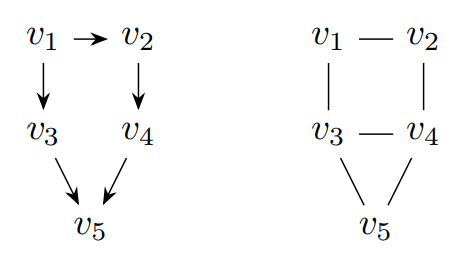
\includegraphics[width=0.4\textwidth]{Figures/State_of_art/graph_moralization.png}
	\caption{Left: A directed acyclic graph (DAG) $\mathcal{D}$; Right: The moral graph of $\mathcal{D}$}
	\label{fig:moralization}
\end{figure}

For a given DAG, the set of ancestors of a vertex $j$, denoted by $\text{an}(j)$, includes all vertices $i$ such that $i \rightarrow j$. Similarly, the set of descendants of a vertex $i$, denoted by $\text{de}(i)$, includes all vertices $j$ such that $i \rightarrow j$. The set of non-descendants of $i$ is $\text{nd}(i) = V \setminus (\text{de}(i) \cup {i})$. A set $A \subseteq V$ is called ancestral if it contains the parents of all its members (\citet{ben2015high}). 

\section{Directed Acyclic Graphs (DAGs) and Notational Conventions}

In equation \ref{ltx}, the vector $\varepsilon$ is defined as the product of the transpose of a lower-triangular matrix $\mathbf{L}$ and the vector $(X_1, \ldots, X_q)^\top$ of random variables:

\begin{equation} \label{ltx}
	\mathbf{L}^T(X_1,...,X_q)^T = \epsilon
\end{equation}

The matrix $\mathbf{L}$ is $(q, q)$ lower-triangular, reflecting an assumed ordering of parent variables. Specifically, $\mathbf{L}$ consists of coefficients ${L_{ij}}$ where $L_{ij} \neq 0$ if and only if $i \rightarrow j$, with diagonal elements set to 1 ($L_{ii} = 1$). The vector $\varepsilon$ represents error terms and is modeled as a $(q, 1)$ vector with a multivariate normal distribution, $\varepsilon \sim \mathcal{N}_q(0, \mathbf{D})$. Here, $\mathbf{D} = \text{diag}(\sigma^2)$ is a diagonal matrix, and $\sigma^2$ is a $(q, 1)$ vector of conditional variances, with each element $\sigma_j^2$ representing the variance of $X_j$ conditioned on its parent variables, denoted as $\text{pa}(j)$, and the matrix $\Omega$.

From the above setup, the precision matrix $\Omega$ can be expressed as:

\begin{equation} \label{omega}
	\mathbf{\Omega} = \mathbf{L}\mathbf{D}^{-1}\mathbf{L}^T
\end{equation}

Equation \ref{omega} is referred to as the modified Cholesky decomposition of $\Omega$, a method that decomposes the precision matrix into the product of a lower-triangular matrix and its transpose, along with a diagonal matrix. The terms $\prec j \succ = \text{pa}(j)$ and $\prec j \succ = \text{pa}(j) \times j$ refer to the set of parent nodes for a given node $j$ and the combination of parent nodes and $j$ itself, respectively. This decomposition allows for a re-parametrization of $\Omega$ using the Cholesky parameters ${ (\sigma_j^2, \mathbf{L}_{\prec j]}), j = 1, \ldots, q }$, where:

\begin{equation} \label{L-Sigma}
	\begin{split}
		\mathbf{\Sigma} = \Omega^{-1}  \\
		\mathbf{L}_{\prec j]} = -\mathbf{\Sigma}^{-1}_{\prec j \succ} \mathbf{\Sigma}_{\prec j]} \\
		\sigma^2_j = \mathbf{\Sigma}_{jj | pa(j)} 
	\end{split}
\end{equation}

with $\mathbf{L}_{\prec j]}$ and $\sigma_j^2$ providing specific information about the dependence structure and conditional variances within the model (\citet{castelletti2021bayesian}). 

A joint distribution that embodies the conditional independence structure represented by a DAG $\mathcal{D}$ is said to be Markov with respect to $\mathcal{D}$. Additionally, if the distribution is Gaussian, its covariance matrix $\mathbf{\Sigma}$, as well as its prevision matrix $\mathbf{\Omega}=\mathbf{\Sigma}^{-1}$, will live in a subspace of the set of symmetric and positive definite matrices because of the constraints imposed by the DAG itself (\citet{peluso2020compatible}).

\section{Markov Equivalence in Graphical Models}

In a noncausal context, Directed Acyclic Graphs are used to represent the conditional independencies between variables through the concept of d-separation (\citet{neuberg2003causality}). When the faithfulness assumption is met, these independencies align precisely with those derived from the joint distribution of the variables. However, it is important to note that multiple DAGs can represent the same set of conditional independencies, making it impossible to distinguish between them using observational data alone (\citet{castelletti2018learning}). 

Moreover, all DAGs that encapsulate the same conditional independencies form what is known as a Markov equivalence class. This class is represented by a Completed Partially Directed Acyclic Graph (PCDAG), also known as an essential graph (EG). 

In practice, the exact structure of the DAG that governs the joint distribution of observed data is often unknown. Consequently, the objective from a noncausal perspective is to identify the underlying EG, which captures the equivalence class of DAGs consistent with the observed conditional independencies (\citet{castelletti2018learning}). 

By definition, two DAGs are Markov equivalent if and only if they have the same skeleton and the same v-structures (\citet{verma2022equivalence}). 
Moreover, the completed PCDAG of a DAG $\textit{D}$, denoted as $\textit{C}$, is a PCDAG that has the same skeleton as $\textit{D}$, and an edge is directed in $\textit{C}$ if and only if it has the same orientation in every equivalent DAG of $\textit{D}$.

The Markov equivalence class of a Directed Acyclic Graph $D$, denoted by $[D]$, comprises all DAGs that are Markov equivalent to $D$. DAGs within the same equivalence class share two key properties (\citet{peluso2020compatible}):
\begin{enumerate}
	\item they have the same skeleton, meaning they are identical when ignoring the direction of the edge;
	\item they have the same immoralities, which are subgraphs of the form $i \rightarrow j \leftarrow z$, with $i, j, z \in V$.
\end{enumerate}

Since it is impossible to distinguish between Markov equivalent graphs using observational data alone, it is essential to ensure score equivalence. This requirement states that any two Markov equivalent DAGs, $\mathcal{D}$ and $\mathcal{D}'$, should have the same marginal likelihood. Mathematically, this is expressed as $\text{BF}_{\mathcal{D},\mathcal{D}'}(Y) = 1$ for all $\mathcal{D} \in [\mathcal{D}']$, where BF denotes the Bayes factor.

A prior distribution that realizes score equivalence is termed compatible. This compatibility ensures that, when using compatible parameter priors, the posterior probabilities of Markov equivalent DAGs will only differ based on their prior probabilities. In other words, the prior beliefs about the structures influence the posterior probabilities, while the observational data alone cannot distinguish between them (\citet{peluso2020compatible}). 

Consider two DAGs $\mathcal{D}_1 = (V,E_1)$ and $\mathcal{D}_2 = (V,E_2)$, where $V = {A, B}$, specifically, $E_1 = {(B,A)}$, and $E_2 = {(A,B)}$. In other words, $\mathcal{D}_1$ represents $A \leftarrow B$ and $\mathcal{D}_2$ represents $A \rightarrow B$. These DAGs are trivially equivalent as they both represent alternative factorizations of the same unconstrained joint distribution of $A$ and $B$.

No amount of observational data, whether finite or infinite, can determine the correct orientation of the edge between $A$ and $B$. Due to their observational equivalence, the marginal likelihoods of $\mathcal{D}_1$ and $\mathcal{D}_2$ are identical. Consequently, the Bayes Factor for comparing these two DAGs will always be one, regardless of the sample size $n$ (\citet{peluso2020compatible}).

\section{Introduction to Markov Chain Monte Carlo (MCMC) Methods}

Markov chain Monte Carlo draw samples from a distribution by running a cleverly constructed Markov chain for a long time. There are many ways of constructing these chains, but all of them, including the Gibbs sampler, are special core of the general framework of Metropolis and Hastings (\citet{gilks1995introducing}). 

For the \textit{Metropolis-Hastings} algorithm, at each time $t$, the next state $X_{t+1}$ is chosen by first sampling a candidate point $Y$ from a proposal distribution $q(.|X)$. This proposal may depend on the current point $X_t$. The candidate point Y is then accepted with probability $\alpha(X_t,Y)$ where (\citet{gilks1995markov}):

\begin{equation} \label{ratio}
	\alpha(X,Y)=min \biggl(1, \frac{\pi(Y)q(X|Y)}{\pi(X)q(Y|X)} \biggr )
\end{equation}

In this expression, $\pi(Y)$ represents the target distribution we wish to sample from. If the candidate point is accepted, the next state becomes $X_{t+1}=Y$. If the candidate is rejected the chain does not move, i.e. $X_{t+1}=X_t$. 

The Gibbs Sampler algorithm is employed to iteratively draw values from the posterior distribution by sampling from the full conditionals. Fortunately, for this specific application, they can be readily recovered in a closed form. The Gibbs sampler is a technique for generating random variables from the posterior distribution indirectly, without having to calculate the density. It generates a sample from $f(x)$ by sampling instead from the conditional distributions $f(x|y)$ and $f(y|x)$t, which are often known in statistical models (\citet{casella1992explaining}).

\subsection{PAS algorithm}

Bayesian model selection is a statistical approach that evaluates and compares different models to identify the one that best explains the observed data. This process involves calculating the likelihood of each model given the data, incorporating prior beliefs about the models and their parameters, and updating these beliefs in light of the observed evidence (\citet{godsill2001relationship}). 

In the context of model selection, each candidate model 
k is associated with a likelihood function $p(y | \theta_k,, k)$, which depends on an (unknown) set of parameters $\theta_k$. Here, $k \in \{1,\ldots, M\}$ represents the index of the model among $M$ possible models. The parameters $\theta_k$ are generally multivariate, with potentially different dimensionality and support $\chi_k$ for different models. \hfill \break 

To incorporate prior knowledge, a prior distribution $p(\theta_k | k)$ is assigned to each parameter vector and a prior distribution $p(k)$ to the model index $k$. The posterior probability of model $k$ given the observed data $y$ is then given by:

\begin{equation} \label{pas-post}
	p(k | y) = \frac{p(y|k)p(k)}{p(y)}
\end{equation}

where $p(y |k)$ is the marginal likelihood of the data under model $k$. It can be expressed as:

\begin{equation} 
	p(y|k)=\int_{\chi_k} p(y|\theta_k,k)p(\theta_k|k) d\theta_k
\end{equation}

In addition, $p(y)$ is the normalizing constant given by:

\begin{equation}
	p(y)=\sum^M_{k=1}p(y|k)p(k)
\end{equation}

which ensures that the posterior probabiliites sum to one across all models. 

To estimate the posterior model probabilities, one common approach is to use independent MCMC chains for each model. This method involves running separate MCMC simulations for the parameters of each model and then combining these results to estimate the posterior probabilities. 
Alternatively, a more integrated approach involves performing MCMC simulations over both the model parameters and the model number. If one can draw random samples $(\theta_i^k,k_i)$ from the joint posterior distribution $p(\theta_k,k|y)$, then Monte Carlo estimate for posterior quantities can be readily computed. 
In cases where there is a nested structure among the parameters of competing models, direct MCMC approaches are often preferred.

Among the various Markov Chain Monte Carlo methods used for model sampling, the reversible jump sampler stands out as one of the most flexible and popular. This approach, initially explored by \citet{carlin1995bayesian}, involves defining a product space that includes all possible model parameters and a model indexing variable. 

The reversible jump sampler can be viewed as a special case of the Metropolis–Hastings algorithm, where a specific type of proposal distribution is employed. This proposal distribution allows the sampler to explore different models by proposing jumps between them. 

When the parameters are a priori independent of one another and of $\theta_k$, the posterior distribution can be expressed in terms of the composite model space.

Specifically, the posterior distribution $p(k,\mathbf{\theta}|y)$ can be rewritten as:

\begin{equation}
	p(k, \mathbf{\theta} |y) = \frac{p(y|k,\theta_k) p(\theta_k|k) \prod_{i \neq k} p(\theta_i | k)}{p(k)p(y)}
\end{equation}

where $p(\theta_i|k)$ represents the prior for the parameters $\theta_i$ that are not included in the model $k$. The term $p(\theta_{-k}|\theta_k,k)$, because of prior independence among parameters, simplifies to:

\begin{equation}
	p(\theta_{-k}|\theta_k,k) =\prod_{i \neq k} p(\theta_i | k)
\end{equation}

where $\theta_{-k}$ denotes the set of parameters excluding $\theta_k$.

A key advantage of the composite model space is that the dimension of the parameter space remains fixed, even as the model index $k$ varies. This happens because, although the model index $k$ may vary, the parameter space is defined to include all possible parameters $\theta$ across all models. Then, each specific model $k$ only activates a subset of these parameters ($\theta_k$), while the remaining parameters $(\theta_{-k})$ do not contribute to the likelihood. Consequently, the overall dimensionality of the parameter space does not increase as different models are explored.
This characteristic allows the use of standard MCMC procedures, such as Gibbs sampling or Metropolis–Hastings algorithms, under typical convergence conditions. 

The convergence properties of the reversible jump MCMC method, as formulated in this specific manner, can be directly inherited from the Metropolis-Hastings algorithm applied to the fixed-dimensional composite space. In this approach, the composite space sampler ensures that the Markov chain has desirable convergence properties.

Specifically, the concepts of irreducibility and aperiodicity of the composite space sampler are inherited. Irreducibility ensures that every state (or model in this case) in the parameter space can be reached from any other state, given enough time. Aperiodicity ensures that the chain does not get trapped in cycles, and the return times to a state are not periodic but rather vary. These properties together guarantee that the Markov chain will converge to the target distribution, which is the posterior distribution over models and parameters. 

In practical scenarios, the ideal scheme for reversible jump MCMC, where the full posterior conditional distribution is known, is often not feasible. However, many models exhibit what can be termed as partial analytic structure. This means that while the full posterior conditional distribution might not be available for all parameters, it is available for some subset of parameters in the new model $k'$. Specifically, if the parameters of the new model $k'$ is denoted as $\theta_{k'}$, the conditional distribution $p((\theta_{k'})_U | (\theta_{k'})_{-U},k',y)$ might be available, where $U$ is a subset of the parameter indices.  \hfill \break

When transitioning from the current model $k$ to the new model $k'$, one effective approach is to use the following reversible jump proposal distribution:
\begin{enumerate}
	\item \textbf{Set common parameters}: set the subset of parameters $(\theta_{k'})_{-U}$ in the new model $k'$ equal to the subset $(\theta_{k})_{-U}$ from the current model $k$. This ensures that these parameters are matched between models;
	\item \textbf{Propose remaining parameters}: propose the remaining parameters $(\theta_{k'})_{U}$ for the new model $k'$ from their full conditional distribution $p((\theta_{k'})_{U} | (\theta_{k'})_{-U},k',y)$. \hfill 
\end{enumerate}

Hence, the acceptance probability for such a proposal is given by:

\begin{equation}
	\alpha = min \biggl \{ 1, \frac{p(k' | (\theta_{k'})_{-U} = (\theta_k)_{U,y})q(k;k')}{p(k|(\theta_k)_{-U,y}q(k';k))} \biggr \}
\end{equation}  

Thus, the proposal probability is independent of parameter values. 
This partial analytic structure approach enables efficient reversible jump sampling by leveraging available conditional distributions for subsets of parameters and maintaining consistency in parameter dimensions between models. The acceptance probability remains independent of the specific parameter values and focuses on model proposal distributions and the posterior odds ratio.

\subsection{Prior specification}

In Bayesian graphical models, prior distributions must be specified for both the parameter vector $\mathbf{\theta}$ and the overall DAG structure. The parameter vector $\mathbf{\theta}$ is composed of the coefficient matrix $\mathbf{L}$ and the diagonal matrix $\mathbf{D}$ of conditional variances.
Two key issues arise in assigning priors:

\begin{enumerate}
	\item \textbf{Consistency Across Markov Equivalence Classes}:  DAGs that belong to the same Markov equivalence class should receive the same prior distribution. This ensures that the prior assignment is compatible across equivalent structures;
	\item \textbf{Efficient Prior Specification}: It is essential to be able to specify prior distributions using a minimal number of direct assessments. This simplifies the process and ensures that the prior information can be effectively incorporated into the model. 
\end{enumerate}

Both of these issues will be addressed to ensure that prior assignments are both consistent and manageable.

A Directed Acyclic Graph is termed complete when it contains all possible arcs between variables, meaning there are no missing edges. 
Complete DAG models for a set of variables $\mathbf{X}$ encode the same assertions of conditional independence—namely, none. In a complete DAG, every variable is directly connected to every other variable, implying no conditional independencies.
One important assumption in this context is that complete DAG models represent the same set of distributions. This implies that data cannot distinguish between two complete DAG models since all possible dependencies are included, making them equivalent in the distributions they represent. 

This leads to the important assumptions outlined by \citet{geiger2002parameter}, which clarify the implications of complete DAG models for inference and model equivalence:

\begin{enumerate}
	\item \textbf{Likelihood modularity}:  for every two DAG models $m_1$ and $m_2$ for $\mathbf{X}$ such that $X_i$ has the same parents in $m_1$ and $m_2$, the local distributions for $x_i$ in both models are the same, namely, $p(x_i|\mathbf{pa}_i^m,\theta_i, m^h_1) = p(x_i|\mathbf{pa}_i^m,\theta_i, m^h_2) \  for  \ all \  X_i \in \mathbf{X}$;
	\item \textbf{Prior modularity}: for every two DAG models $m_1$ and $m_2$ for $\mathbf{X}$ such that $X_i$ has the same parents in $m_1$ and $m_2$, $p(\theta_i |m_1^h) = p(\theta_i |m_2^h)$; 
	\item \textbf{Global parameter independence}: for every DAG model m for $\mathbf{X}$, $p(\theta_m|m^h)=\prod^n_{i=1}p(\theta_i|m^h)$. 
\end{enumerate}

Together, the first two assumptions mean that the local distribution for a variable $x_i$  and its parameter priors depend only on its parent variables, not on the entire structure of the DAG. This modularity simplifies the process of specifying priors and computing likelihoods, as one needs to consider only the local parent-child relationships. Specifically, the likelihood modularity means that the overall model can be built in a modular fashion. Each local distribution can be specified independently as long as the parent sets are maintained. Even if two models have different overall structures, as long as the local parent-child relationships for a variable are identical, the conditional distributions for that variable will be identical. \hfill \break

Additionally, global parameter independence  states that parameters associated with different parts of the DAG are independent. It implies that the parameters $\theta_i$ associated with each variable  $X_i$  are independent of each other given the model $m$. The prior knowledge or beliefs about the parameters of one variable do not influence the parameters of another variable.
This assumption allows for separate handling and estimation of parameters for different variables, facilitating a more straightforward and modular approach to modeling.
Moreover, it excludes, for example, the possibility that two local distributions share a common parameter. 

The assumptions above made have a significant consequence: specifying a parameter prior $p(\theta_{mc}|m_{hc})$ for a complete DAG model $m_c$ implicitly defines a prior $p(\theta_m | m_h)$ for any DAG model $m$ among the exponentially many possible DAG models. This framework allows  to use a manageable number of direct assessments to derive all the necessary priors for searching the model space efficiently. 

To compute $p(\theta_i \mid m_h)$, we identify a complete DAG model $m_c(i)$ where the parent set of $x_i$ in model $m$ matches that in model $m_c(i)$, i.e., $\text{Pa}i^m = \text{Pa}i^{m_c(i)}$. The prior $p(\theta_{m_c(i)} \mid m_{h_c(i)})$ is derived from $p(\theta_{m_c} \mid m_{h_c})$ for every pair of complete DAG models. Due to global parameter independence, $p(\theta_{m_c(i)} \mid m_{h_c(i)})$ is a product, one term of which is $p(\theta_i \mid m_{h_c(i)})$.

Finally, due to prior modularity, $p(\theta_i \mid m_h)$ is equal to $p(\theta_i \mid m_{h_c(i)})$. This modularity ensures that the local distribution for each variable depends only on its parent set, simplifying the computation. 

Given these assumptions every independence equivalent DAG model have the same marginal likelihood. 
In addition, it can be shown that the only pdf which satisfies global parameter independence, when the number of coordinates is bigger than two, is the Normal-Wishard distribution also known as DAG-Wishard. For this prior it is known that the local parameter independence must hold (\citet{geiger2002parameter}). 

An important feature of the DAG-Wishard distribution is that node-parameters $\{(\mathbf{D}_{jj}, \mathbf{L}_{\prec j]}), j = 1, \ldots, q\}$ are a priori independent with distribution:

\begin{equation} \label{L-Sigma}
	\begin{split}
		\mathbf{D}_{jj} | G \sim I-Ga  \biggl( \frac{1}{2} a^G_j, \frac{1}{2}\mathbf{U}_{jj | pa_G (j)} \biggr ) \\
		\mathbf{L}_{\prec j]} | \mathbf{D}_{jj}, G \sim N_{pa_G (j)} \Bigl(- \mathbf{U}^{-1}_{\prec j \succ} \mathbf{U}_{\prec j ]}, \mathbf{D}_{jj}\mathbf{U}^{-1}_{\prec j \succ} \Bigr )
	\end{split}
\end{equation}

Unfortunately, DAG-Wishart distributions with arbitrarily chosen hyperparameters will lead to incompatible priors for model selection, because they assign different marginal likelihoods to Markov equivalent graphs. To overcome this difficulty, a constructive method to specify DAG-Wishart priors whose suitably constrained shape hyperparameters ensure compatibility for DAG model selection has been proposed. 
Specifically, $a_j^G = a + |pa_G (j)| -q + 1$ where q is the number of parameters (\citet{peluso2020compatible}).  

\paragraph{Prior on DAG structures}
Let's consider $S_q$, the space of all Directed Acyclic Graphs on $q$ nodes. For a given DAG $\mathcal{D} = (V, E) \in S_q$, we define $S_{\mathcal{D}}$ as the 0-1 adjacency matrix of its skeleton. The skeleton is the undirected graph obtained by ignoring the directionality of the edges in $D$. Specifically, for each pair of nodes $(u, v)$, the corresponding element in $S_D$ is $S_{\mathcal{D}_{u,v}} = 1$ if there is an edge between $u$ and $v$ (regardless of its direction), and $0$ otherwise.

Given a prior probability of edge inclusion, denoted as $\eta \in (0, 1)$, each entry $S_{D_{u,v}}$ for $u > v$ follows an independent and identically distributed Bernoulli distribution: $S_{\mathcal{D}_{u,v}} \mid \eta \sim \text{Ber}(\eta)$. This implies that the likelihood of observing a specific skeleton $S_\mathcal{D}$, given $\eta$, is:

\begin{equation}
	p(\mathbf{S}^\mathcal{D}|\pi)=\pi^{|\mathbf{S}^\mathcal{D}|}(1-\pi)^{\frac{q(q-1)}{2}-|\mathbf{S}^\mathcal{D}|}
\end{equation}

where $|S_{\mathcal{D}}|$ denotes the number of edges in $\mathcal{D}$, and $\frac{q(q-1)}{2}$ is the maximum number of possible edges in a DAG with $q$ nodes.

To incorporate uncertainty about the inclusion probability $\eta$, a Beta prior is placed on $\eta$, i.e., $\eta \sim \text{Beta}(a, b)$ (\citet{castelletti2023bayesian}). 

\subsubsection{Introduction to Markov Chain Monte Carlo (MCMC) Methods}

\paragraph{Marginal likelihood} Given that the Cholesky parameters $\mathbf{L}$ and $\mathbf{D}$ are independent across nodes $j=1,...,q$, the marginal likelihood can be computed by factorizing the integral over the joint distribution into a product of integrals, with each integral corresponding to a single node $j$.

\begin{equation} \label{m-like}
	\begin{split}
		m(\mathbf{X}|\mathcal{D}) & = \int p(\mathbf{X} | \mathbf{D}, \mathbf{L}, \mathcal{D})p(\mathbf{D}, \mathbf{L}) d(\mathbf{D}, \mathbf{L}) \\
		& = \int \prod_{j=1}^q p(\mathbf{X}_j | \mathbf{X}_{pa(j)}, \mathbf{L}_{\prec j ]}, \mathbf{D}_{jj})p(\mathbf{L}_{\prec j ]}, \mathbf{D}_{jj})d \mathbf{D}_{jj}d \mathbf{L}_{\prec j ]} \\
		& = \prod_{j=1}^q \int p(\mathbf{X}_j | \mathbf{X}_{pa(j)}, \mathbf{L}_{\prec j ]}, \mathbf{D}_{jj})p(\mathbf{L}_{\prec j ]}, \mathbf{D}_{jj})d \mathbf{D}_{jj}d \mathbf{L}_{\prec j ]} \\
		& = \prod_{j=1}^q m(\mathbf{X}_j | \mathbf{X}_{pa(j)})
	\end{split}
\end{equation}

The marginal likelihood $m(\mathbf{X}|\mathcal{D})$, as in $\textit{Equation}$ \ref{m-like}, is now expressed as a product over individual terms corresponding to each node $j$, reflecting the factorization of the joint likelihood (\citet{castelletti2022bcdag}). 

\paragraph{MCMC structure}
To estimate the joint posterior distribution of DAG structures and their associated parameters, the goal is to sample from $p(\mathcal{D}, \mathbf{L}, \mathbf{D} \mid \mathbf{X})$, which is proportional to the product of the likelihood $f(\mathbf{X} \mid D, \mathbf{L}, \mathbf{D})$, the prior distribution $p(\mathbf{L}, \mathbf{D} \mid \mathcal{D})$ for the DAG parameters, and the prior $p(\mathcal{D})$ for the DAG structure:

\begin{equation}
	p(\mathbf{D}, \mathbf{L}, \mathcal{D} | \mathbf{X}) \propto f(\mathbf{X} | \mathbf{D}, \mathbf{L}, \mathcal{D})p(\mathbf{D}, \mathbf{L} | \mathcal{D})p(\mathcal{D})
\end{equation}

where $\mathbf{X}$ represents the data matrix with $n$ observations and $q$ variables.

The proposed sampling method utilizes a reversible jump Markov Chain Monte Carlo algorithm. This approach effectively navigates the model space by considering the Partial Analytic of the DAG-Wishart distribution (\citet{castelletti2022bcdag}). This formulation simplifies the computation of the posterior distribution by integrating out parameters analytically, thus reducing the computational burden and enhancing the efficiency of the sampler.

\paragraph{Proposal distribution}

The proposal distribution determines how new candidate DAGs are generated from the current DAG during the sampling process. Ideally, the proposal distribution should be designed to balance two key objectives: it should explore the DAG space efficiently, meaning it should propose significant and varied changes to the graph structure, and it should maintain a reasonable acceptance rate, ensuring that the proposed DAGs are likely to be accepted in the MCMC process.

Three types of local operators are employed:

\begin{enumerate}
	\item Inserting a directed edge ($\text{Insert}_D$);
	\item Deleting a directed edge ($\text{Delete}_D$);
	\item Reversing the direction of a directed edge ($\text{Reverse}_D$). 
\end{enumerate}

These operations allow to generate a set of valid operators, denoted as $\mathcal{O}_{\mathcal{D}}$, where each operator results in a new graph that is still a valid DAG.

For any given DAG $D \in S_q$, the set $\mathcal{O}_{\mathcal{D}}$ consists of all possible operators that can be applied to $\mathcal{D}$ without violating the acyclic structure. From this set, a new DAG $\mathcal{D}'$ is proposed by uniformly sampling one of the valid operators from $\mathcal{O}_{\mathcal{D}}$. This ensures that the probability of transitioning from $\mathcal{D}$ to a specific successor DAG $\mathcal{D}'$ is given by $q(\mathcal{D}' \mid \mathcal{D}) = \frac{1}{|\mathcal{O}_{\mathcal{D}}|}$, where $|\mathcal{O}_D|$ is the total number of valid operators applicable to $\mathcal{D}$. This approach ensures that each potential DAG transition is equally likely (\citet{castelletti2022bcdag}). 

\subsection{Poisson process}

After discussing the foundational aspects of MCMC, it's important to explore more specialized algorithms that can handle model selection and varying dimensions. One such approach is the birth-death MCMC algorithm, which captures the dynamics of adding or removing components from the model. To introduce this, the Poisson process is considered—a stochastic process that plays a key role in modeling the transitions between states in the birth and death framework, providing the necessary probabilistic structure.

Poisson data represent counts of events where there is no predefined upper limit on how many events can occur over a given period or within a specific area. For data to follow a Poisson distribution, four key assumptions must hold (\citet{rosner2021bayesian}):

\begin{enumerate}
	\item  The events must be "rare", meaning that the likelihood of observing two or more events in a very small time interval or space is extremely low, decreasing rapidly as the interval or area shrinks;
	\item The occurrence of events must be stationary. This means that the probability of observing a certain number of events in a fixed time interval or area remains consistent, regardless of when or where that interval or area is located;
	\item Events in different, non-overlapping intervals of time or distinct regions of space must be independent of each other, an assumption known as "independent increments";
	\item The probability of a single event occurring in a small interval or region should be directly proportional to the length of the interval or the size of the region. When these conditions are met, the number of events in any fixed interval or region follows a Poisson distribution with a mean equal to the product of the constant event rate and the length or size of the interval or region.
\end{enumerate}

Consequently, a counting process $\{N_t, t \geq 0\}$ is said to be a Poisson process with rate $\lambda > 0$ if the following properties hold true:

\begin{itemize}
	\item $N_0 = 0$;
	\item $\{N_t, t \geq 0 \}$ has independent increments;
	\item $P(N_{t+h}-N_t = 1) = \lambda h + o(h)$;
	\item $P(N_{t+h}-N_t \geq 2) = o(h)$.
\end{itemize}

Here it is stated that the probability of observing exactly one event in a short interval is proportional to the length of the interval, while the probability of observing multiple events in the same interval is negligible.

The Poisson process is characterized by the memoryless property, which means that the likelihood of an event occurring in the future is unaffected by the history of past events. In other words, the process essentially "restarts" at each point in time. This property implies that the time until the next event, known as the interarrival time, follows an exponential distribution.

In fact, the exponential distribution is the only one having the memoryless property, by consequence, its probability distribution does not depend on how much time has already passed. Formally, if $T$ represents the time until the next event, then for any $t \geq 0$, the distribution of $T$ is:

\begin{equation}
	P(T > t + s | T > s) = P(T > t)
\end{equation}

which shows that the probability of waiting an additional time $t$ does not depend on how long was already waited. 

\subsection{Birth and Death process}

A birth and death process is a type of continuous-time Markov chain used to model systems where entities arrive ("births") and depart ("deaths") over time. The process is defined by a state space ${0, 1, 2, \ldots}$ representing the number of entities in the system at any given time. The dynamics of the process are governed by transition rates: $\lambda_n$ denotes the rate at which births occur when the system is in state $n$, and $\mu_n$ denotes the rate at which deaths occur from state $n$.

In this framework, the waiting time for a new arrival/birth is
exponentially distributed with parameter $\lambda_n$ and is independent of the waiting time for a new departure/death, which is exponentially distributed with parameter $\mu_n$.

Formally, a birth and death process with birth and death parameters $\{\lambda_n\}^{\infty}_{n=0}$ and $\{\mu_n\}^{\infty}_{n=0}$ is a continuous-time Markov chain with $\mathbb{S} = \{0,1,2, \ldots\}$ for which transitions from state n may go only to either state n-1 or state n+1. Transition rates and probabilities are given by:

\begin{itemize}
	\item $v_0 = \lambda_0$;
	\item $v_i = \lambda_i + \mu_i, \ i>0$;
	\item $P_{01} = 1$;
	\item $P_{i,i+1}=\frac{\lambda_i}{\lambda_i + \mu_i}, P_{i, i-1} = \frac{\mu_i}{\lambda_i + \mu_i}, \ i>0$
\end{itemize}

where $P_{01}$ is the transition probability from state 0 to 1. Moreover, $v_0$ is the total transition rate out of state 0, which is equal to the birth rate $\lambda_0$, since state 0 only transitions to state 1. Instead, for $i>0$, $v_i$ is the total transition rate out of state $i$, calculated as the sum of the birth rate $\lambda_i$ and the death rate $\mu_i$.

\subsection{BDMCMC}

The birth-death MCMC sampling algorithm operates within a continuous-time birth-death Markov process framework. This algorithm explores the graph space by performing link addition (birth) or removal (death) operations.

In this process, for a given graph $\mathcal{D} = (V, E)$ and precision matrix $\Omega$, each link in the graph can be removed as an independent Poisson process with a specific death rate $\delta_e(\Omega)$ for each link $e \in E$. The total death rate for all links is given by $\delta(K) = \sum_{e \in E} \delta_e(\Omega)$. Conversely, the birth rate $\beta_e(\Omega)$ for a potential link $e \notin E$ is similarly defined, with the overall birth rate being $\beta(\Omega) = \sum_{e \notin E} \beta_e(\Omega)$ (\citet{mohammadi2015bdgraph}).

Since birth and death events are modeled as independent Poisson processes, the time between successive events follows an exponential distribution with a mean of $1 / (\beta(\Omega) + \delta(\Omega))$. This time represents the waiting period for the next event in the process.

The probabilities of observing a birth or death event are computed as follows: 

\begin{itemize}
	\item Probability of adding a link $e$ that is not currently in the graph is:
	
	
	\begin{equation}
		Pr(\text{birth of link e}) = \frac{\beta_e(\Omega)}{\beta(\Omega)+\delta(\Omega)}\ \text{for each $e \notin E$}
	\end{equation}
	
	\item Probability of removing a link $e$ that is already present in the graph is:
	
	\begin{equation}
		Pr(\text{death of link e}) = \frac{\delta_e(\Omega)}{\beta(\Omega)+\delta(\Omega)}\ \text{for each $e \in E$}
	\end{equation}
	
\end{itemize}

These probabilities and rates guide the algorithm's exploration of the graph space by determining how frequently links are added or removed, facilitating the sampling of graph structures and their associated parameters. 

In the BDMCMC algorithm,  birth and death events are modeled as independent Poisson processes. This means that the timing of these events follows an exponential distribution, where the time between successive events is determined by the rates at which births and deaths occur. Events are distributed randomly over time, and the exponential distribution describes the waiting time between these random events. By carefully adjusting the birth and death rates, the algorithm ensures that these rates are proportional to the likelihood of the respective graph and precision matrix configurations. This setup guarantees that the stationary distribution of the Markov process matches the target posterior distribution of the graph and the precision matrix  (\citet{mohammadi2015bayesian}).

\begin{figure}[h] 
	\centering
	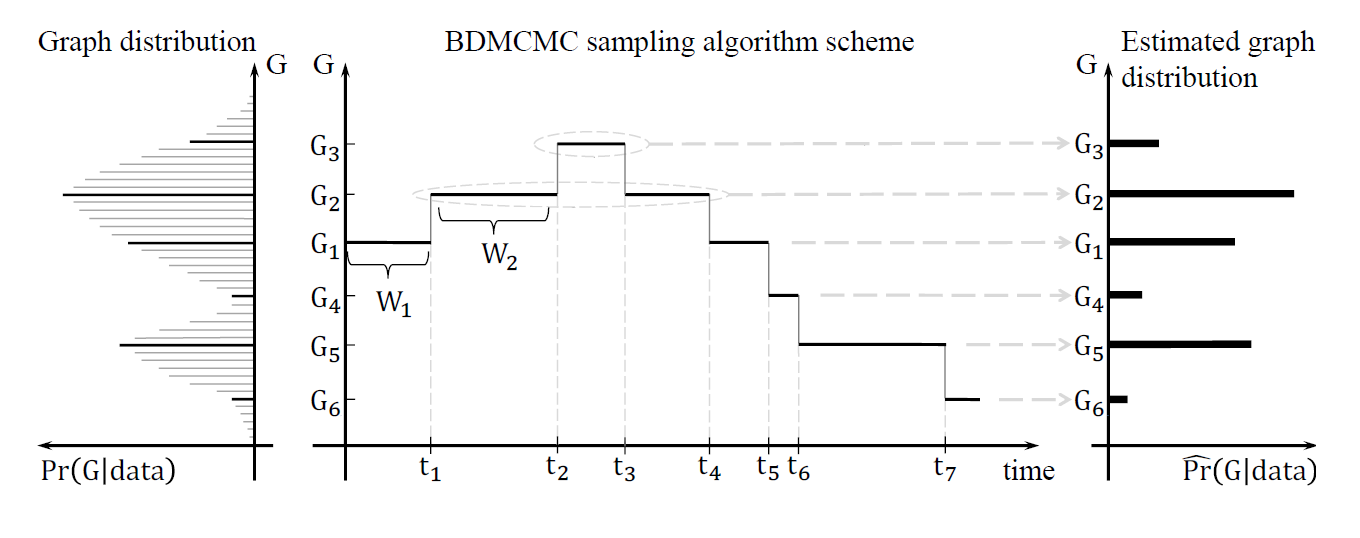
\includegraphics[width=0.9\textwidth]{Figures/State_of_art/BDMCMC_theory.png}
	\caption{The left panel displays the true posterior distribution of the graphs. The middle panel illustrates a continuous-time BDMCMC sampling algorithm, where ${W_1, W_2, \dots}$ represent the waiting times, and ${t_1, t_2, \dots}$ denote the jump times. The right panel shows the estimated posterior probabilities of the graphs.}
	\label{fig:BDMCMC}
\end{figure}

\chapter{MCMC Approaches and Implementation}

Selecting an appropriate DAG model or a set of DAG models given a dataset is a highly complex computational problem. The primary challenge arises from the fact that the number of possible DAG models increases at a rate faster than exponential as the number of variables grows. This exponential explosion in the number of possible models makes exhaustive search and evaluation of every potential DAG impractical for anything beyond a small number of variables (\citet{geiger2002parameter}).

In most cases, the true DAG that represents the underlying data-generating process is unknown, and the challenge of identifying this structure is referred to as structural learning. Within the Bayesian framework, structural learning is approached as a model selection problem. A prior distribution is assigned to the parameter space associated with each potential DAG, known as the parameter prior. This prior, when integrated with the data, yields a marginal likelihood for each DAG. By combining these marginal likelihoods with a prior distribution over the entire space of possible DAGs, one can derive the posterior distribution over the model space. This posterior distribution reflects the updated beliefs about which DAGs are most plausible given the observed data, guiding the selection of the most likely underlying structure  (\citet{peluso2020compatible}).

Search algorithms for DAG structures often use operators designed to transition between DAGs within the same equivalence class, this latter being the set of DAGs that encode the same conditional independence relationships among variables. Under the assumption that the structure represents independencies, applying such an operator does not change the underlying information; it simply generates a different representation of the same state. Consequently, if a search algorithm does not explicitly account for equivalence, it may inefficiently spend computational resources by repeatedly re-scoring DAGs that belong to the same equivalence class. This redundancy is particularly problematic because, for the algorithm to transition from one equivalence class to another, it must often perform multiple moves within the current equivalence class. Therefore, the connectivity of these equivalence classes in the search space is influenced by the specific DAG used to represent the current equivalence class.

When the search operators involve directed edge additions, deletions, and reversals, a score-equivalent criterion complicates the process further. A greedy search algorithm, which seeks to maximize the score at each step, will not distinguish between two equivalent DAGs and may arbitrarily choose between them if their scores are identical. This can lead to inefficiencies where the algorithm repeatedly evaluates the same state, as it might reverse an edge that simply leads to an equivalent DAG, wasting time in the process (\citet{chickering2002learning}).

\section{Adaptive MCMC algorithm}

The adaptive mechanism is designed to enhance the efficiency of exploring DAGs within a Markov Chain Monte Carlo framework by dynamically adjusting proposal probabilities based on estimated posterior probabilities of edge inclusion and non-inclusion. This approach focuses on utilizing the information obtained from a sequence of sampled DAGs to inform and guide the proposal mechanism.
Now, let $\mathcal{D}^{(1)},...,\mathcal{D}^{(t)}$ be a collection of DAGs sampled by the MCMC scheme from the posterior over DAGs $p(\mathcal{D}|Y)$ up to time t (t=1,...,T).

The estimated posterior probability of including the directed edge $u \rightarrow v $, based on the collection $\{\mathcal{D}^{(1)},...,\mathcal{D}^{(t)}\}$, is computed as the average across all samples and is expressed as follows:

$$\hat{p}_{u\rightarrow v} (Y) =\hat{p} (u \rightarrow v | \mathcal{D}^{(1)},...,\mathcal{D}^{(t)}, Y) = \frac{1}{t}\sum^t_{i=1} \mathbbm{1} \{u \rightarrow v  \in \mathcal{D}^{(s)}\}$$ 

where

\begin{equation} \label{posterior-prob}
	\mathbbm{1} \{u \rightarrow v  \in \mathcal{D}^{(s)}\} = \begin{cases}
		1 & \text{if} \  u \rightarrow v \in  \mathcal{D}^{(s)}\\
		0 & \text{if not}
	\end{cases}
\end{equation}

Moreover, $$\hat{p}_{u\nrightarrow v} (Y) =\hat{p} (u \nrightarrow v | \mathcal{D}^{(1)},...,\mathcal{D}^{(t)}, Y) = \frac{1}{t}\sum^t_{i=1} \mathbbm{1} \{u \rightarrow v  \notin \mathcal{D}^{(s)}\} = 1- \hat{p}^{(t)}_{u\rightarrow v} (Y)$$

is defined as the probability of non inclusion of edge $u \rightarrow v $.

When constructing proposals based on the insertion, deletion, or reversal of edges $u \rightarrow v $, the approach ensures that edges with a higher probability $\hat{p}_{u\rightarrow v} (Y)$ are more likely to be included, while edges with a higher probability of non-inclusion $\hat{p}_{u\nrightarrow v} (Y)$ are more likely to be deleted. This strategy leads to a proposal distribution that is not uniform across all possible valid operations but instead focuses on the most promising changes.

Given the current DAG $\mathcal{D}^{(t)}$ three types of operators are considered, namely, Insert $\mathcal{D}^{(t)}$, Delete $\mathcal{D}^{(t)}$ and Reverse $\mathcal{D}^{(t)}$:
\begin{equation}
	\begin{split}
		O_{I\mathcal{D}} &= \{ (u,v) \; \text{such that} \; u \rightarrow v \notin ^{(t)} \; \text{and} \; \text{Insert}_{\mathcal{D}}(u \rightarrow v) \; \text{is valid} \}, \\
		O_{D\mathcal{D}} &= \{ (u,v) \; \text{such that} \; u \rightarrow v \in ^{(t)} \; \text{and} \; \text{Delete}_{\mathcal{D}}(u \rightarrow v) \; \text{is valid} \}, \\
		O_{R\mathcal{D}} &= \{ (u,v) \; \text{such that} \; u \rightarrow v \notin ^{(t)} \; \text{and} \; \text{Reverse}_{\mathcal{D}}(u \rightarrow v) \; \text{is valid} \}.
	\end{split}
\end{equation}

These three sets, $O_{I\mathcal{D}}$, $O_{D\mathcal{D}}$, and $O_{R\mathcal{D}}$, contain candidate edges for the insertion, deletion, and reversal of directed edges, respectively. For each of these operations, the associated proposal probabilities can be computed as follows:

First, for each candidate edge $\sigma = (u, v) \in O_{\mathcal{D}}$, calculate the estimated posterior probability of edge inclusion, $\hat{p}^{(t)}_{u \rightarrow v}(Y)$, based on the current collection of samples. The proposal probability for the insertion of this edge is then defined as:
\begin{equation} \label{proposal-prob-add} q_{\sigma} \propto \frac{\hat{p}^{(t)}{u \rightarrow v}(Y) + C}{1 - \hat{p}^{(t)}{u \rightarrow v}(Y) + C} \end{equation}

This formulation ensures that edges with higher estimated posterior probabilities are more likely to be selected for inclusion in the proposal.

Second, for each candidate edge $\sigma = (u, v) \in O_{\mathcal{D}}$, compute the estimated posterior probability of edge non-inclusion, $\hat{p}^{(t)}_{u \nrightarrow v}(Y)$. The associated proposal probability for the deletion of this edge is given by:
\begin{equation} \label{proposal-prob-del} q_{\sigma} \propto \frac{\hat{p}^{(t)}{u \nrightarrow v}(Y) + C}{1 - \hat{p}^{(t)}{u \nrightarrow v}(Y) + C} = \frac{1 - \hat{p}^{(t)}{u \rightarrow v}(Y) + C}{\hat{p}^{(t)}{u \rightarrow v}(Y) + C} \end{equation}

Here, the proposal probability is inversely related to the estimated probability of edge inclusion, favoring the deletion of edges that are less likely to be included.

Finally, for each candidate edge $\sigma = (u, v) \in O_{R\mathcal{D}}$, compute the estimated posterior probability of edge non-inclusion, $\hat{p}^{(t)}{u \nrightarrow v}(Y)$. Note that the reversal of an edge $u \rightarrow v$ can be decomposed into a deletion followed by an insertion, i.e., $Reverse\mathcal{D}(u, v) = Delete\mathcal{D}(u, v) + Insert\mathcal{D}(v, u)$. Next, calculate the updated probability $\hat{p}^{(t+1)}{v \rightarrow u} \mid \text{DeleteD}(u, v) \text{ at time } t$, given by:

$$
\hat{p}^{(t+1)}_{u\rightarrow v} = \frac{1}{t+1}\sum_1^{t}\mathbbm{1}\{u \rightarrow v \in \mathcal{D}^{(s)}\}
$$

The proposal probability for the reversal of the edge is then defined as:

\begin{equation} \label{proposal-prob-reverse}
	q_{\sigma} \propto \frac{1-\hat{p}^{(t)}_{u\rightarrow v} (Y )+C}{\hat{p}^{(t)}_{u\rightarrow v} (Y)+C} = \frac{\hat{p}^{(t+1)}_{v\nrightarrow u} (Y ) \ |  "Delete\mathcal{D}(u,v) \ at \ time \ t"+C}{1-\hat{p}^{(t+1)}_{v\nrightarrow u} (Y) \ | "Delete\mathcal{D}(u,v) \ at \ time \ t"+C} 
\end{equation}

The conditioning on $"Delete\mathcal{D}(u,v) \ at \ time \ t"$ reflects the two-step process involved in the reversal operation. First, the edge $(u,v)$ is deleted at time $t$, which modifies the graph's structure. Following this deletion, the proposal to reverse the edge is based on the addition of the reversed edge $(v,u)$ at time $t+1$. 
As $t \rightarrow \infty$, it follows that $q_{\sigma} \rightarrow 1$. Therefore, $q_{\sigma} = 1$ is set for each $\sigma \in O_{R\mathcal{D}}$.

Next, consider the Metropolis-Hastings ratio, particularly: 

$$
\frac{q(\mathcal{D}^{(\star)})|\mathcal{D}^{(t)})}{q(\mathcal{D}^{(t)})|\mathcal{D}^{(\star)})} \ \ \ \ \ \ (\Delta)
$$

The ratio ($\Delta$) represents the likelihood ratio of transitioning between two DAGs under the proposed changes. Given that each candidate edge operation $\sigma$ (whether insertion, deletion, or reversal) has a corresponding reverse operation, the proposal probabilities $q_{\sigma}$
are constructed to be symmetric with respect to these reverse operations. This symmetry implies that the ratio of proposal probabilities for moving from one DAG $\mathcal{D}^t$ to another $\mathcal{D}^{(s)}$
is exactly balanced by the ratio for the reverse transition. Consequently, this results in $\Delta = 1$, ensuring that the Metropolis-Hastings acceptance ratio is unaffected by the proposal probabilities, thus preserving detailed balance and the correctness of the MCMC sampling procedure.

The adaptivity mechanism allows the algorithm to prioritize operations that are more probable according to the observed data. Additionally, the introduction of a constant ensures that even edges with estimated probabilities of 0 receive a non-zero proposal probability, maintaining the diversity of proposed operations. 

\begin{figure}[h] 
	\centering
	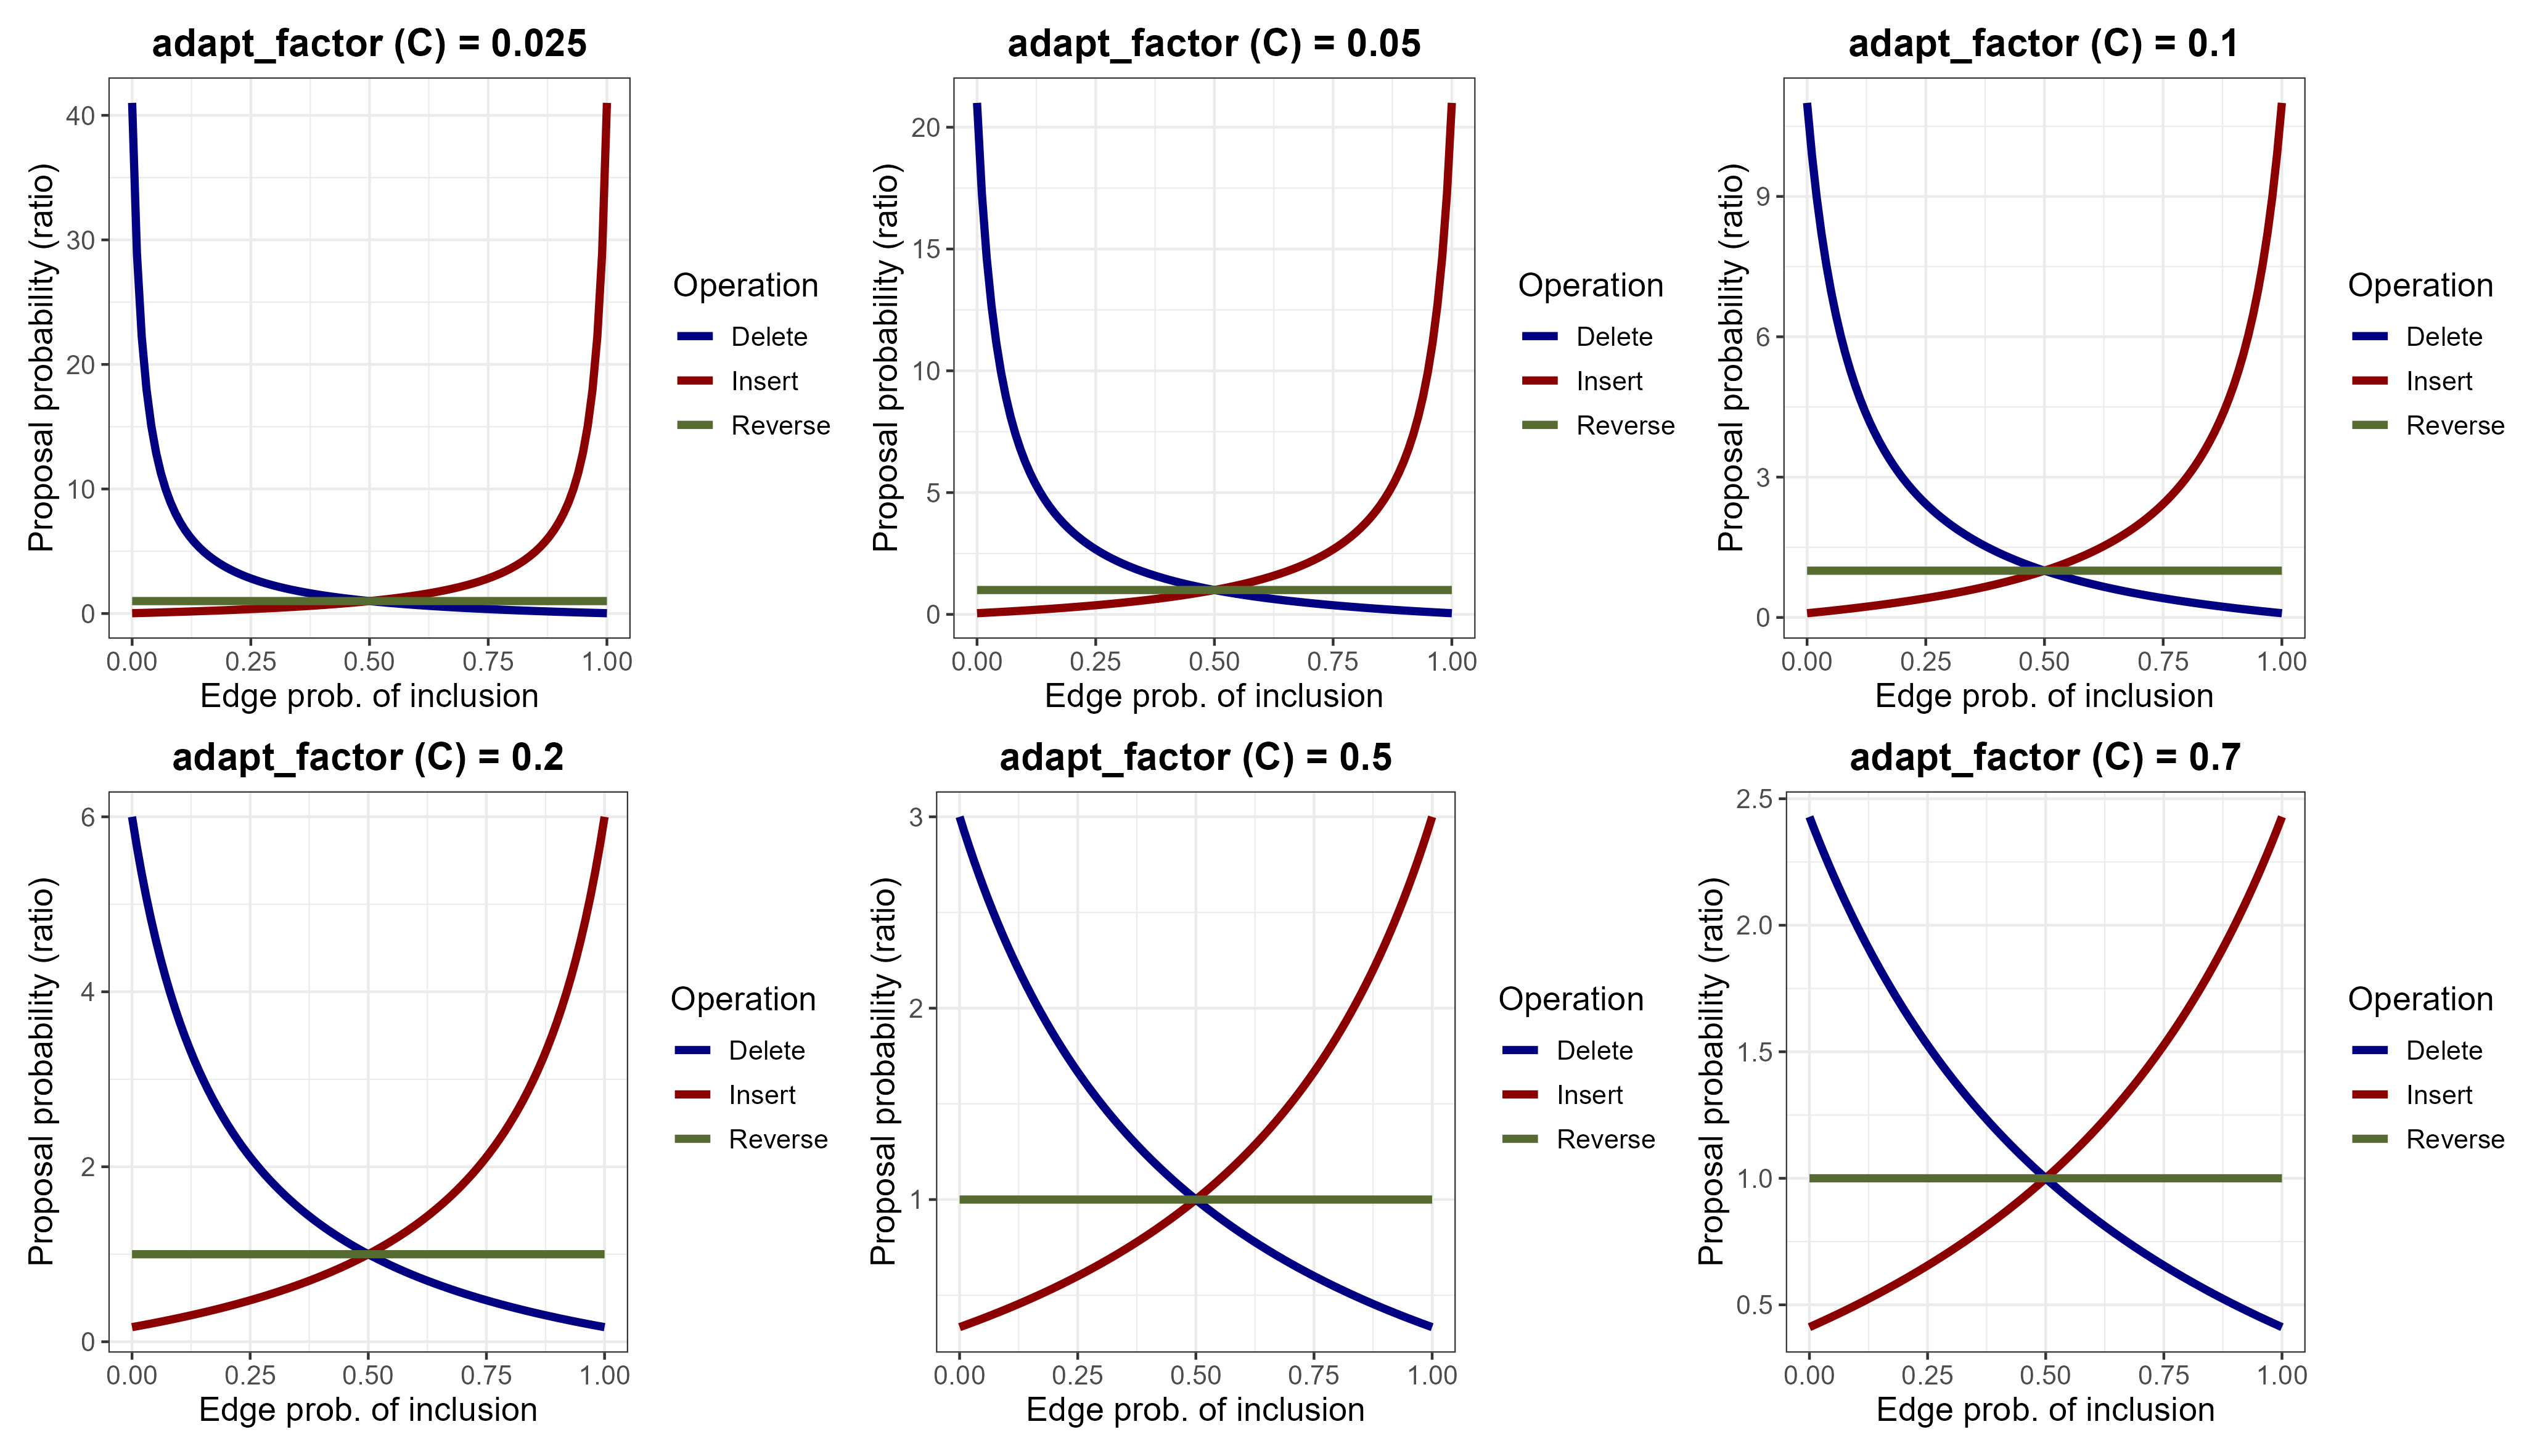
\includegraphics[width=0.75\textwidth]{Figures/Adaptive_behaviour/c_comparison.png}
	\caption{Edge Inclusion Probability Across Varying C Parameter Levels for Addition, Deletion, and Reversal Operations}
	\label{fig:c-comp}
\end{figure}

As illustrated in Fig \ref{fig:c-comp} an increase in the constant $C$ results in a reduction of the range on the y-axis, leading to diminished adaptation to the estimated posterior distribution. Additionally, as $C$ becomes larger, the Reverse operator's influence becomes more pronounced. When the initial probability of an edge is high, the corresponding edge is more likely to be included; conversely, when the probability is low, the edge is more likely to be removed. This relationship explains why the red and blue lines in the figure exhibit a mirrored pattern.

\subsection{Implementation Code}

Building on the MCMC scheme implemented in the BCDAG package (\citet{castelletti2022bcdag}), several modifications were made to incorporate the adaptive mechanism. Specifically, a boolean parameter was introduced within the $\textit{learn\_dag}$ function, allowing for the selection between the standard and adaptive approaches together with the parameter $\textit{adapt\_factor}$. An example is below.

\begin{lstlisting}[language=R]
	out_mcmc = learn_DAG(S = 60000, burn = 5000, a = q, U = diag(1,q)/n, data = X, w = 0.1, fast = TRUE, save.memory = T, adaptive_mcmc = TRUE, adapt_factor = 0.7)
\end{lstlisting}

The adaptation probabilities are determined through a weighted mean approach that combines the previously computed average probabilities with those derived from the most recent DAG proposal. Instead of recalculating the entire graph, which is stored as a three-dimensional array, the algorithm updates a matrix that holds the cumulative mean of the probabilities. This matrix-based computation is more efficient, both in terms of memory usage and processing speed, as it avoids the need to reconstruct or manipulate the full graph structure during each iteration. \hfill \break

The reassessment of the acceptance ratio, specifically $\frac{P(\theta^* | \theta^{(S)})}{P(\theta^{(S)} | \theta^*)}$, is necessary due to the change in how proposal probabilities are assigned under the new adaptive mechanism. Previously, the selection of operations was based on a uniform probability distribution; however, it is now dependent on proposal probabilities that are defined by the weighted mean of past iterations. 

To clarify, consider the computation of the acceptance ratio, starting with the numerator. It outlines all possible operations along with their associated proposal probabilities, given the current structure $\theta^{(S)}$. These probabilities are used as weights to sample the operation that will be performed next. Once an operation is selected, the corresponding proposal probability, located in the relevant row of the table, is used as the value for $P(\theta^* | \theta^{(S)})$ in the acceptance ratio.

In particular, the code operates such that after an operation is proposed and a new DAG is selected, a new table of proposal probabilities is generated. This new table corresponds to the denominator in the acceptance ratio for the current iteration. Within this table, the probability for the specific operation being proposed is identified by selecting the appropriate row corresponding to the current node. If the proposed operation is accepted, this newly constructed table becomes the current table, reflecting the updated DAG structure. This updated table will then be used directly in the next iteration to determine the proposal probabilities for subsequent operations.

By following this approach, only one new table is generated in each iteration, while the other table, depending on whether the operation is accepted or not, either becomes the current table or remains unchanged. This process ensures computational efficiency by avoiding the need to construct multiple tables for each iteration.

\subsection{Algorithm Dynamics and Convergence}

In order to assess the algorithm properties a first comparison was made between the plain mcmc algorithm and its adaptive version. This section focuses on a biological dataset of patients diagnosed with Acute Myeloid Leukemia (AML). The dataset comprises measurements of 18 proteins and phosphoproteins involved in apoptosis and cell cycle regulation. The data was originally made available as supplementary material in the study by \citet{kornblau2009functional}.

\paragraph{Graphsize}

As shown in \textit{Figure} 3.2.1 and 3.2.2, increasing the parameter $C$ leads to convergence of the graph size at a higher value, though it does not reach the levels observed in the standard Metropolis algorithm. This behavior occurs because the proposal probabilities for different edges become more balanced, allowing for a broader distribution of sampling weights. Instead of heavily favoring previously sampled values, the algorithm permits nodes that have not yet been explored to maintain a non-zero probability of being sampled, which increases with $C$. Consequently, a larger portion of the parameter space is explored.

\begin{figure}[!h]
	\centering
	\resizebox{\textwidth}{6.5cm}{  
		\begin{minipage}{\textwidth}
			\centering
			
			% First figure
			\begin{subfigure}[b]{0.45\textwidth}   
				\centering
				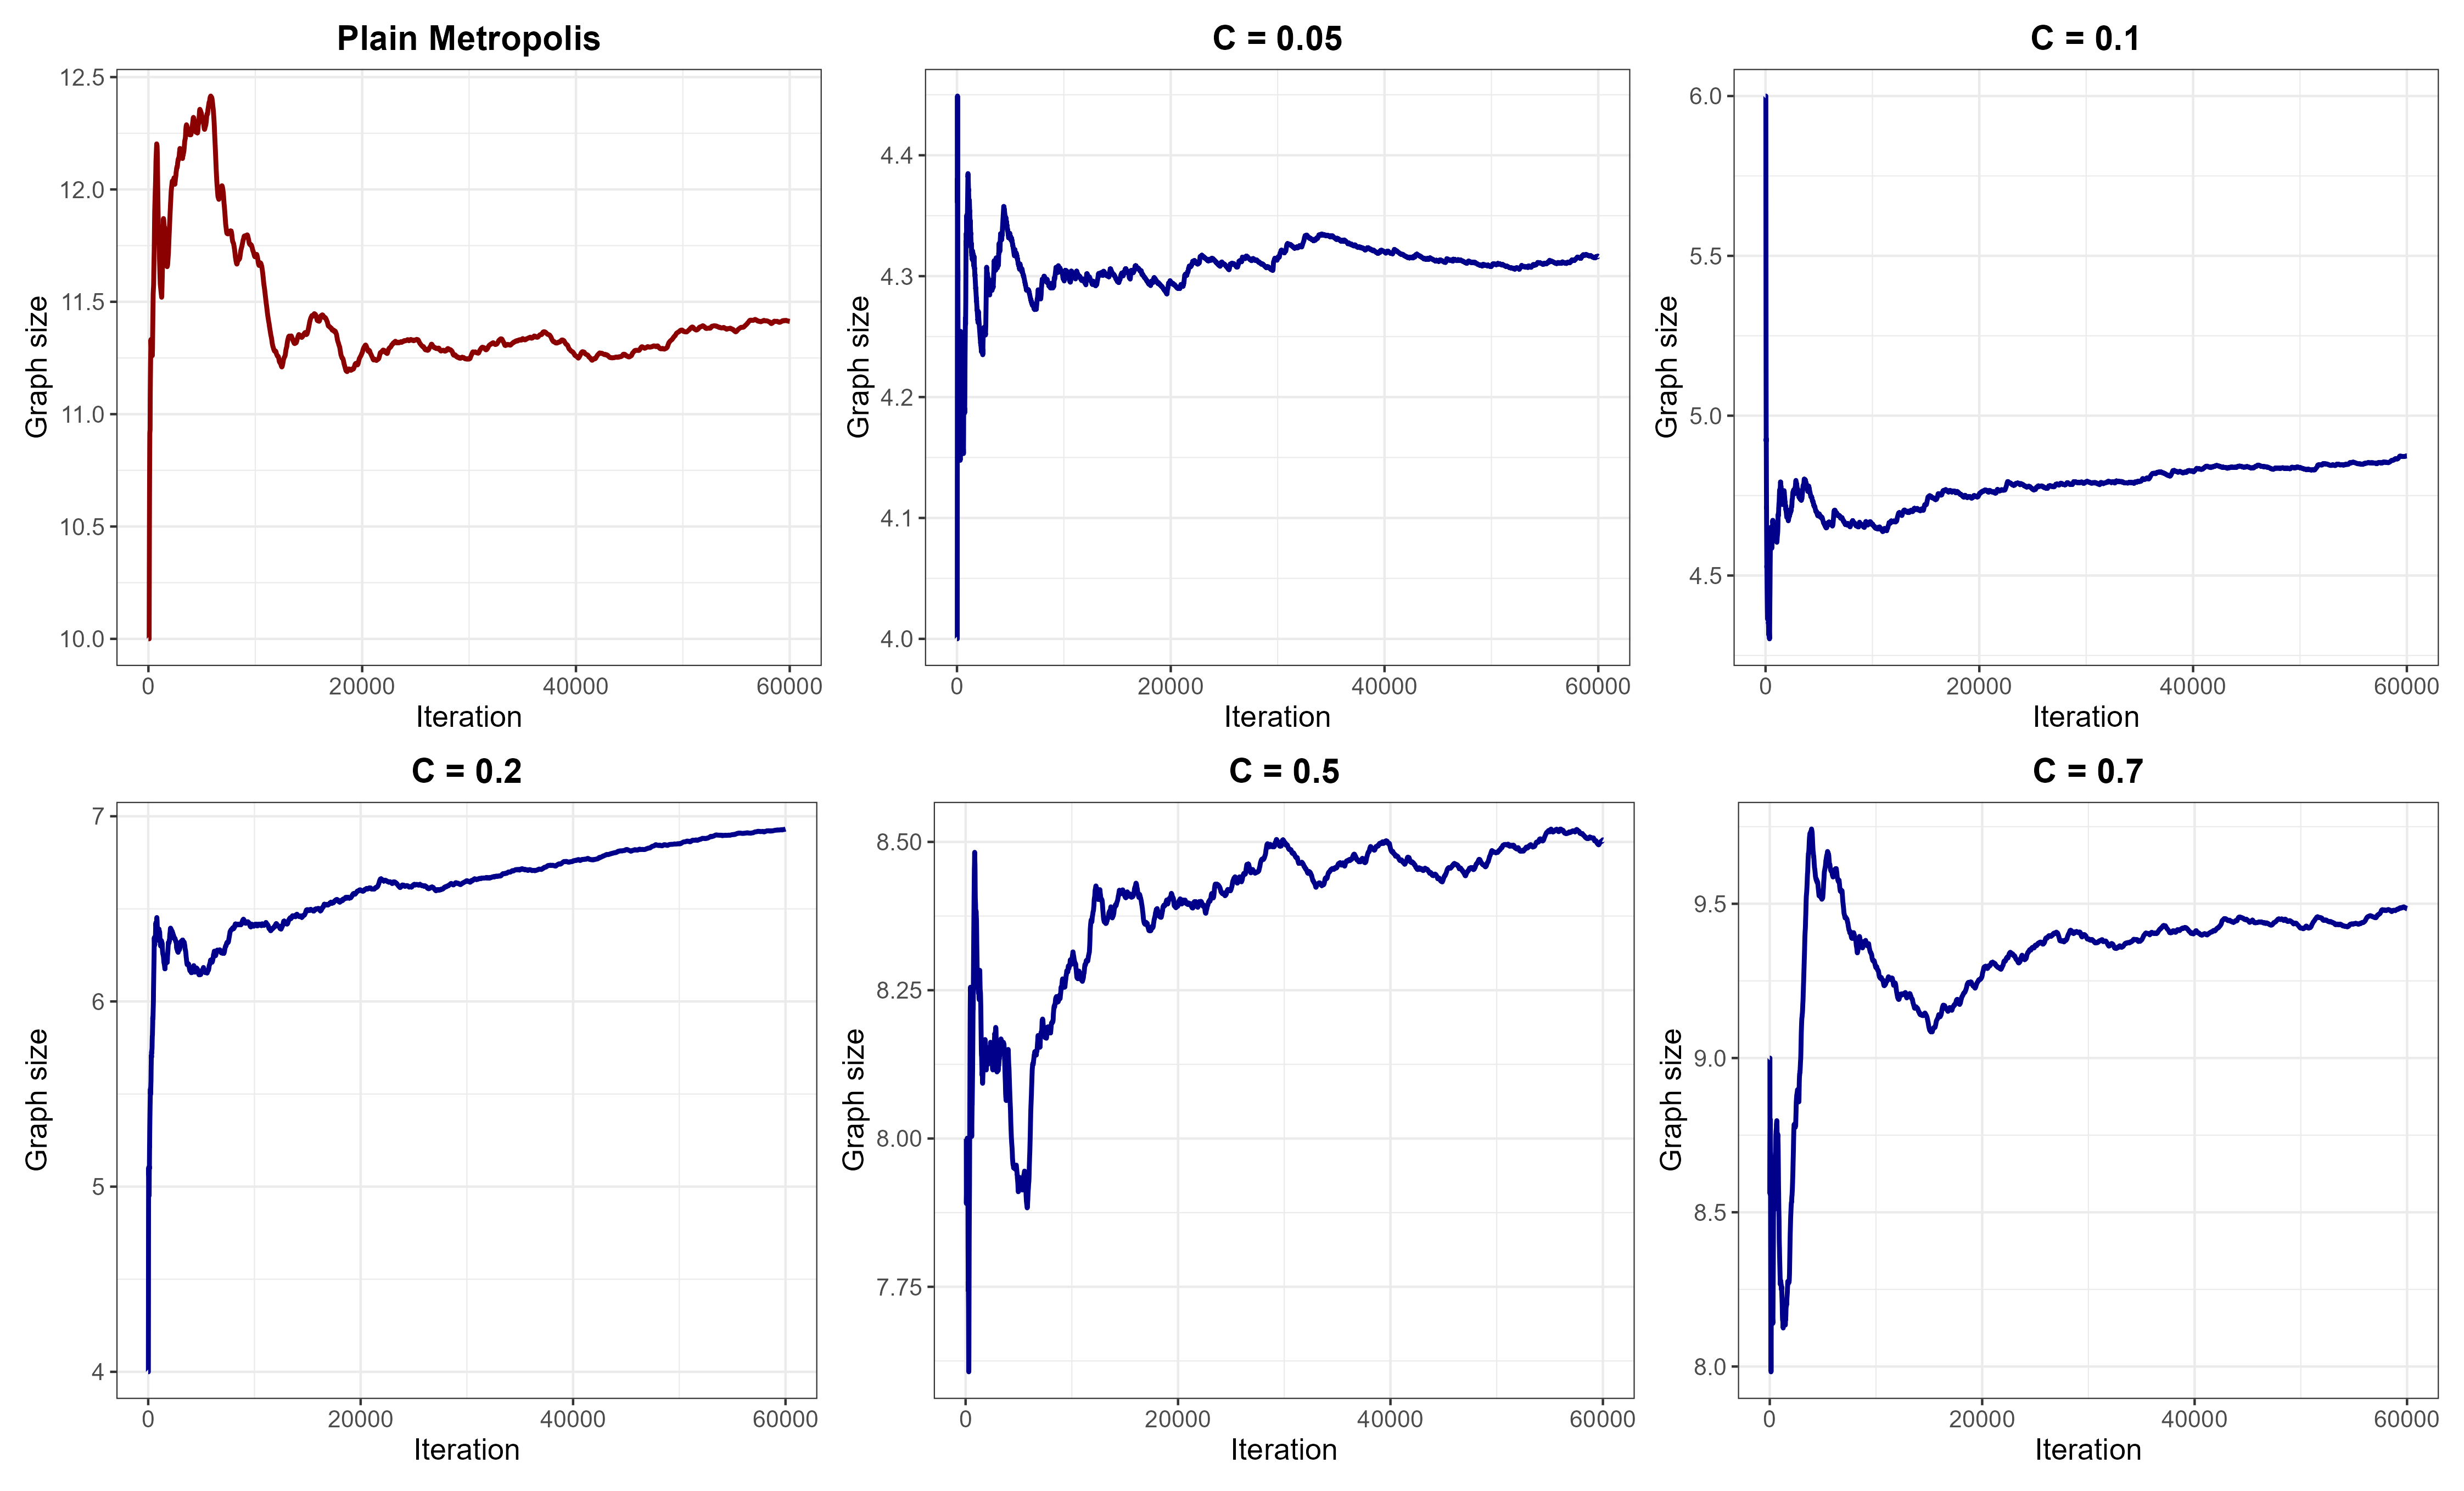
\includegraphics[height=4.1cm]{Figures/Adaptive_behaviour/GraphCum_trace.png}
				%\caption{}
				\label{fig:graphcum-trace}
			\end{subfigure}
			\hspace{0.35cm}  % horizontal space between figures
			% Second figure
			\begin{subfigure}[b]{0.45\textwidth}   
				\centering
				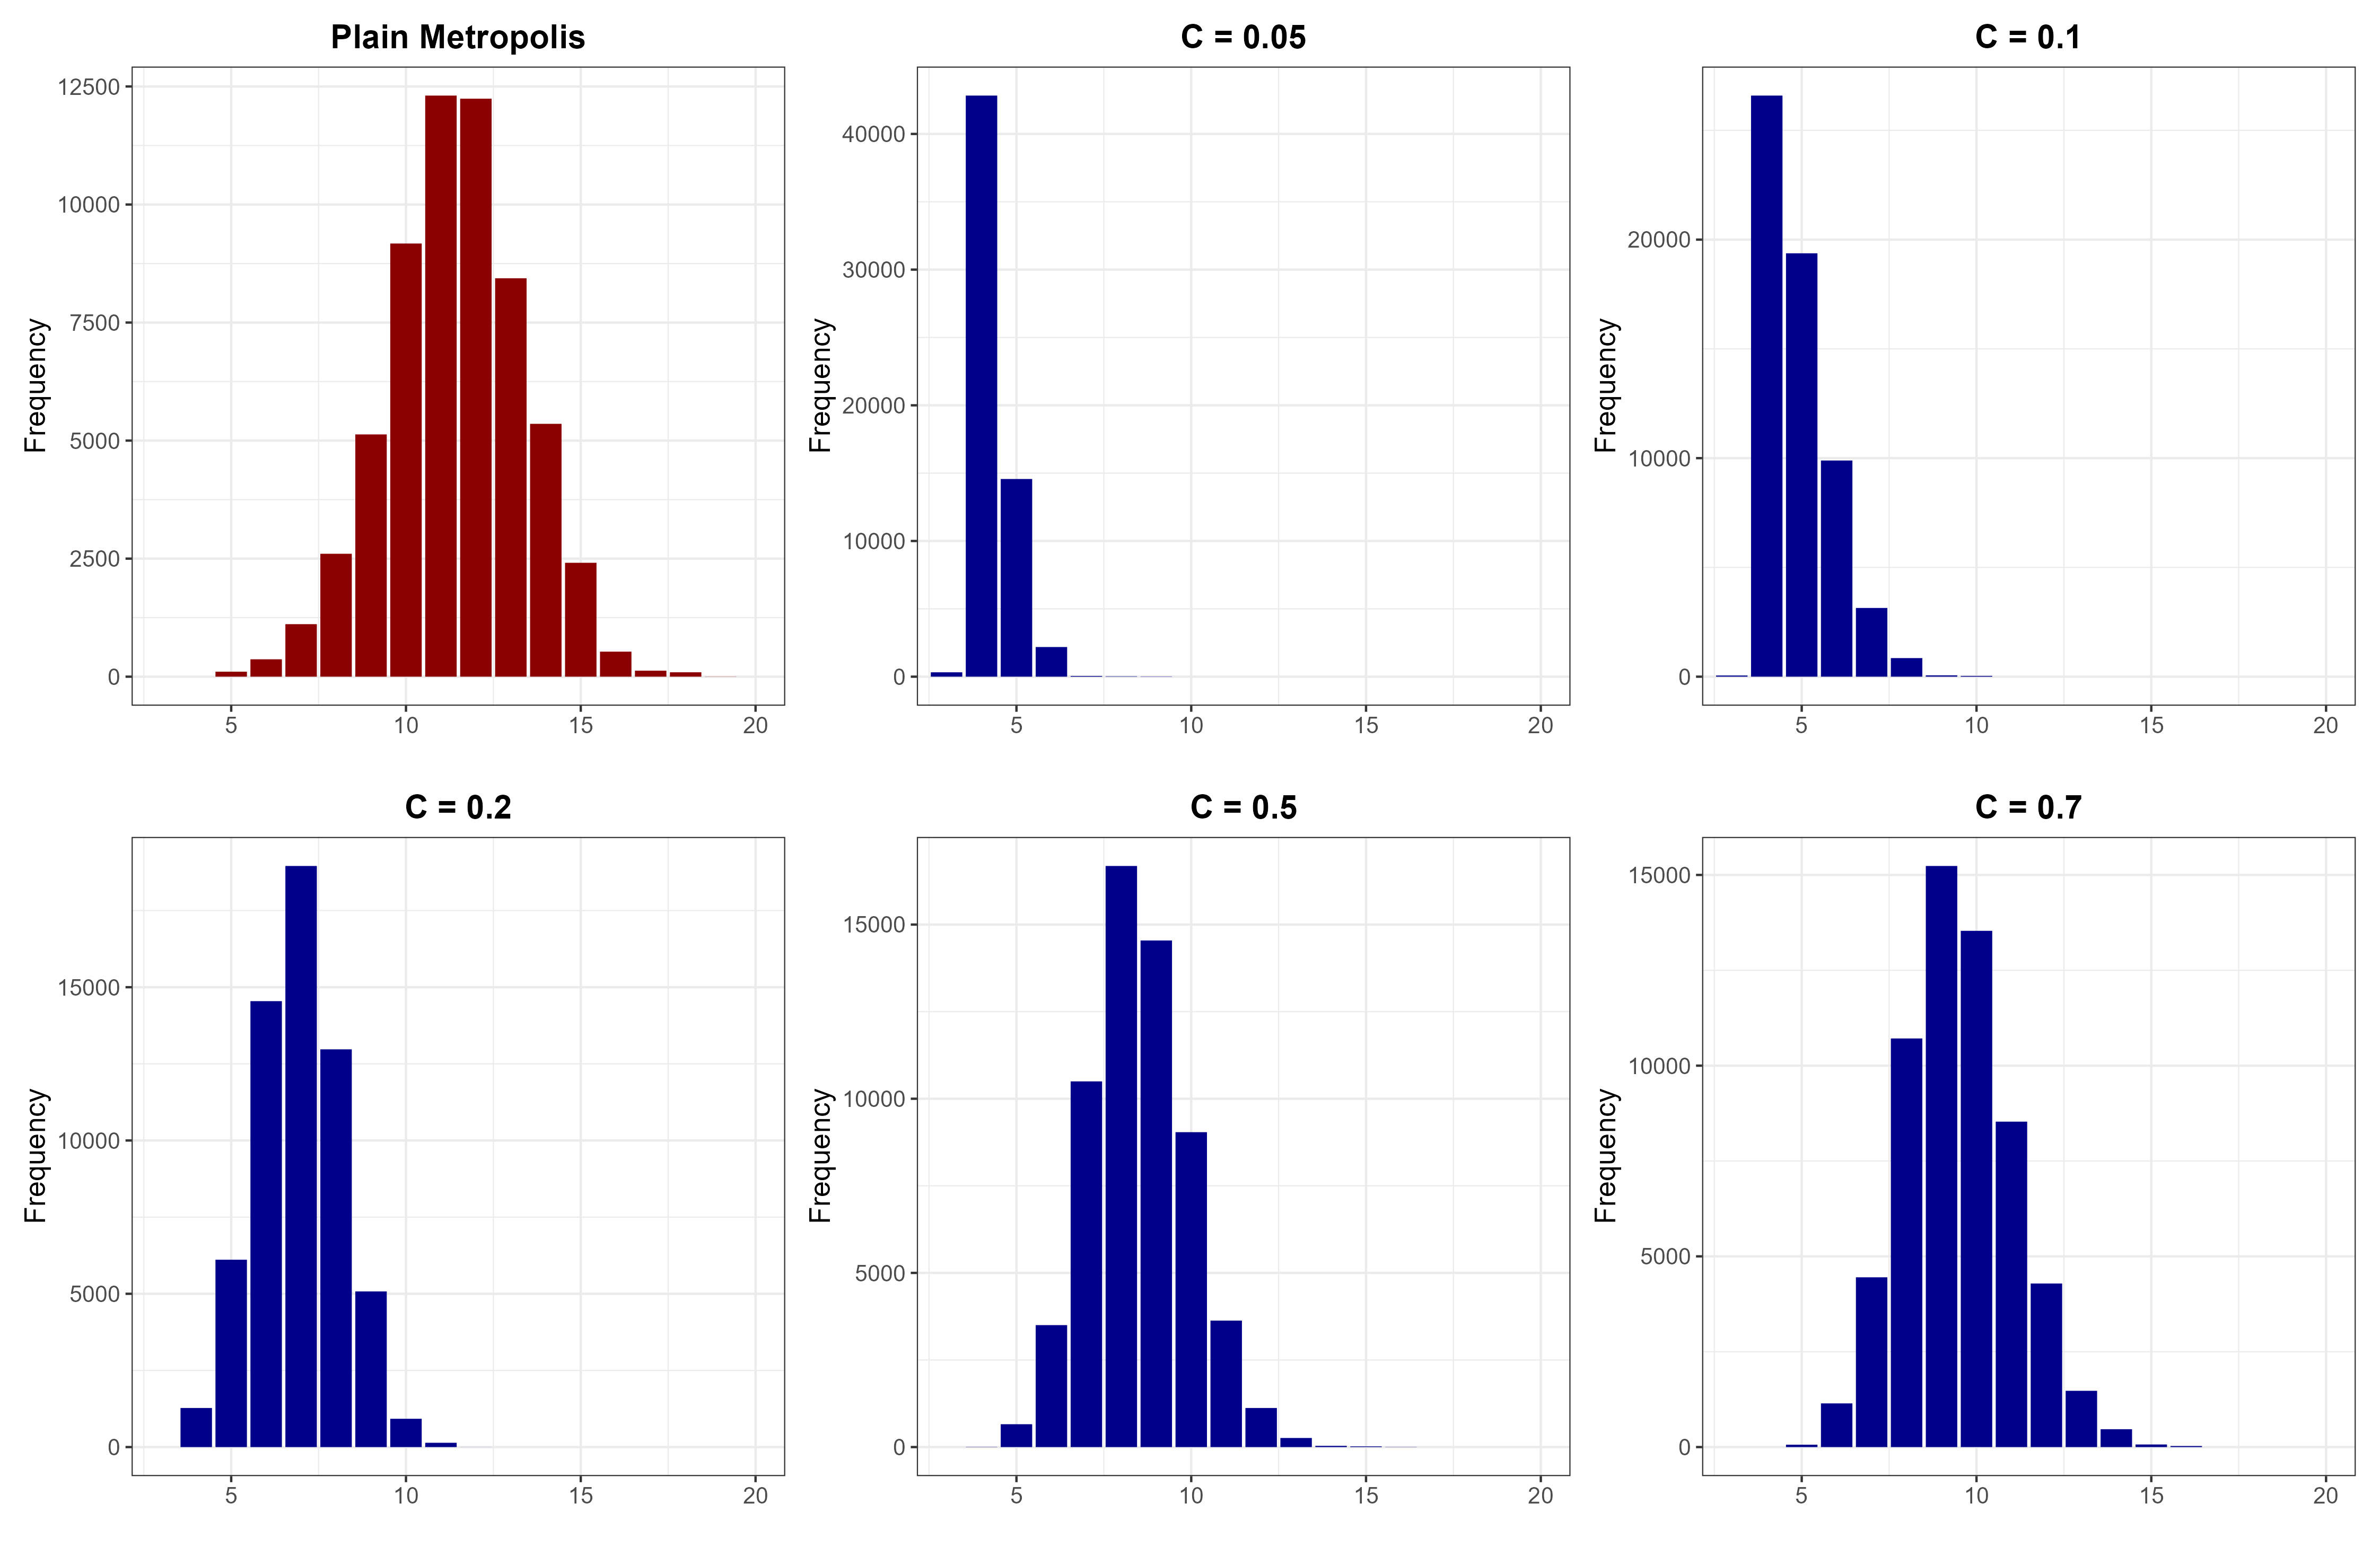
\includegraphics[height=4.1cm]{Figures/Adaptive_behaviour/GraphsizeHist.png}
				%\caption{}
				\label{fig:graphsize-hist}
			\end{subfigure}
			
			\vspace{0.4cm}   %  vertical space between rows 
			
			% Third figure
			\begin{subfigure}[b]{0.45\textwidth}   
				\centering
				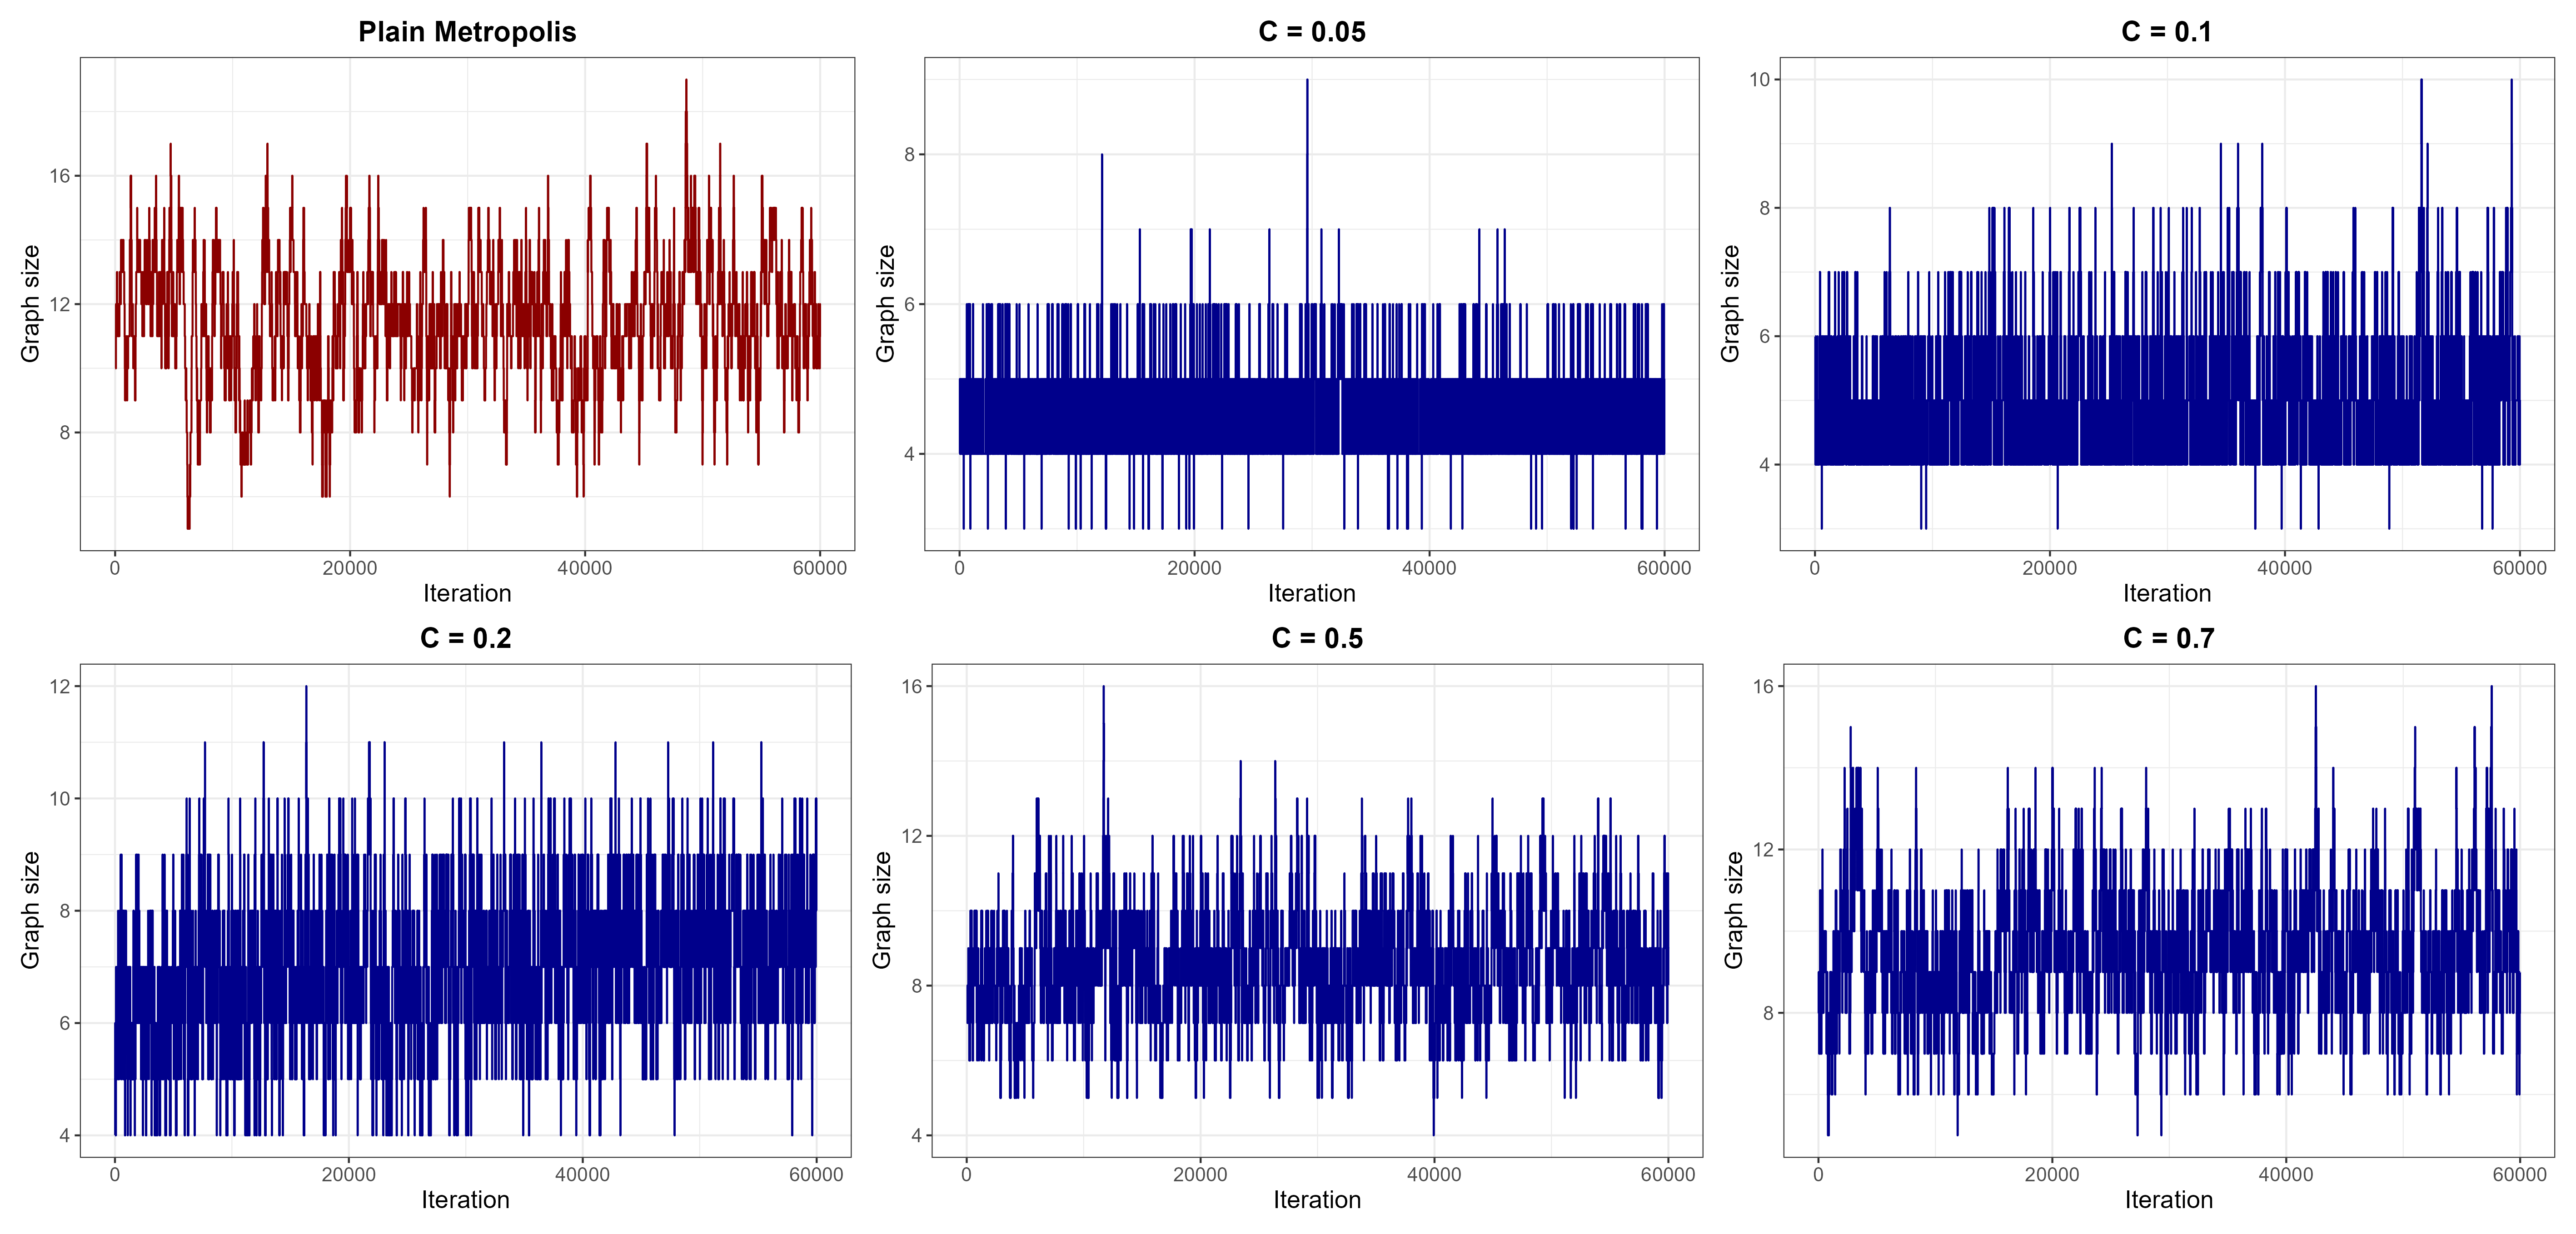
\includegraphics[height=4.1cm]{Figures/Adaptive_behaviour/GraphSize_traceplot.png}
				%\caption{}
				\label{fig:graphsize-trace}
			\end{subfigure}
		\end{minipage}
	}
	\caption{Analysis of graph size dynamics across different values of parameter C to evaluate the Markov chain's mixing behavior. The figures include: (1) a cumulative line plot of graph size, (2) a histogram of graph size distribution, and (3) a trace plot of graph size to assess mixing.}
	\label{fig:complexity}
\end{figure}

Additionally, as illustrated in \textit{Figure} 3.2.3, increasing the parameter $C$ results in greater variation in the graph dimensions explored by the algorithm. With smaller values of $C$, the trace plot remains relatively stable, indicating a high level of correlation and limited exploration of different configurations. In contrast, with larger values of $C$, the algorithm assigns higher proposal probabilities to less frequently visited nodes, leading to a broader exploration of the parameter space and greater variation in the graph dimensions.

\paragraph{Unique graphs}

In Bayesian statistics, an essential consideration when comparing posterior probabilities is the adequacy of the sampling process in exploring the parameter space. An inefficient sampling mechanism, which disproportionately focuses on a confined region of the parameter space, can result in biased posterior probabilities. This bias manifests as an overemphasis on specific models or edges, potentially skewing the results and leading to misleading conclusions. Inadequate exploration of the DAG space may occur if the sampler fails to sufficiently investigate alternative graph structures. This limitation can prevent the identification of models that might more accurately capture the underlying data. 

\begin{figure}[h] 
	\centering
	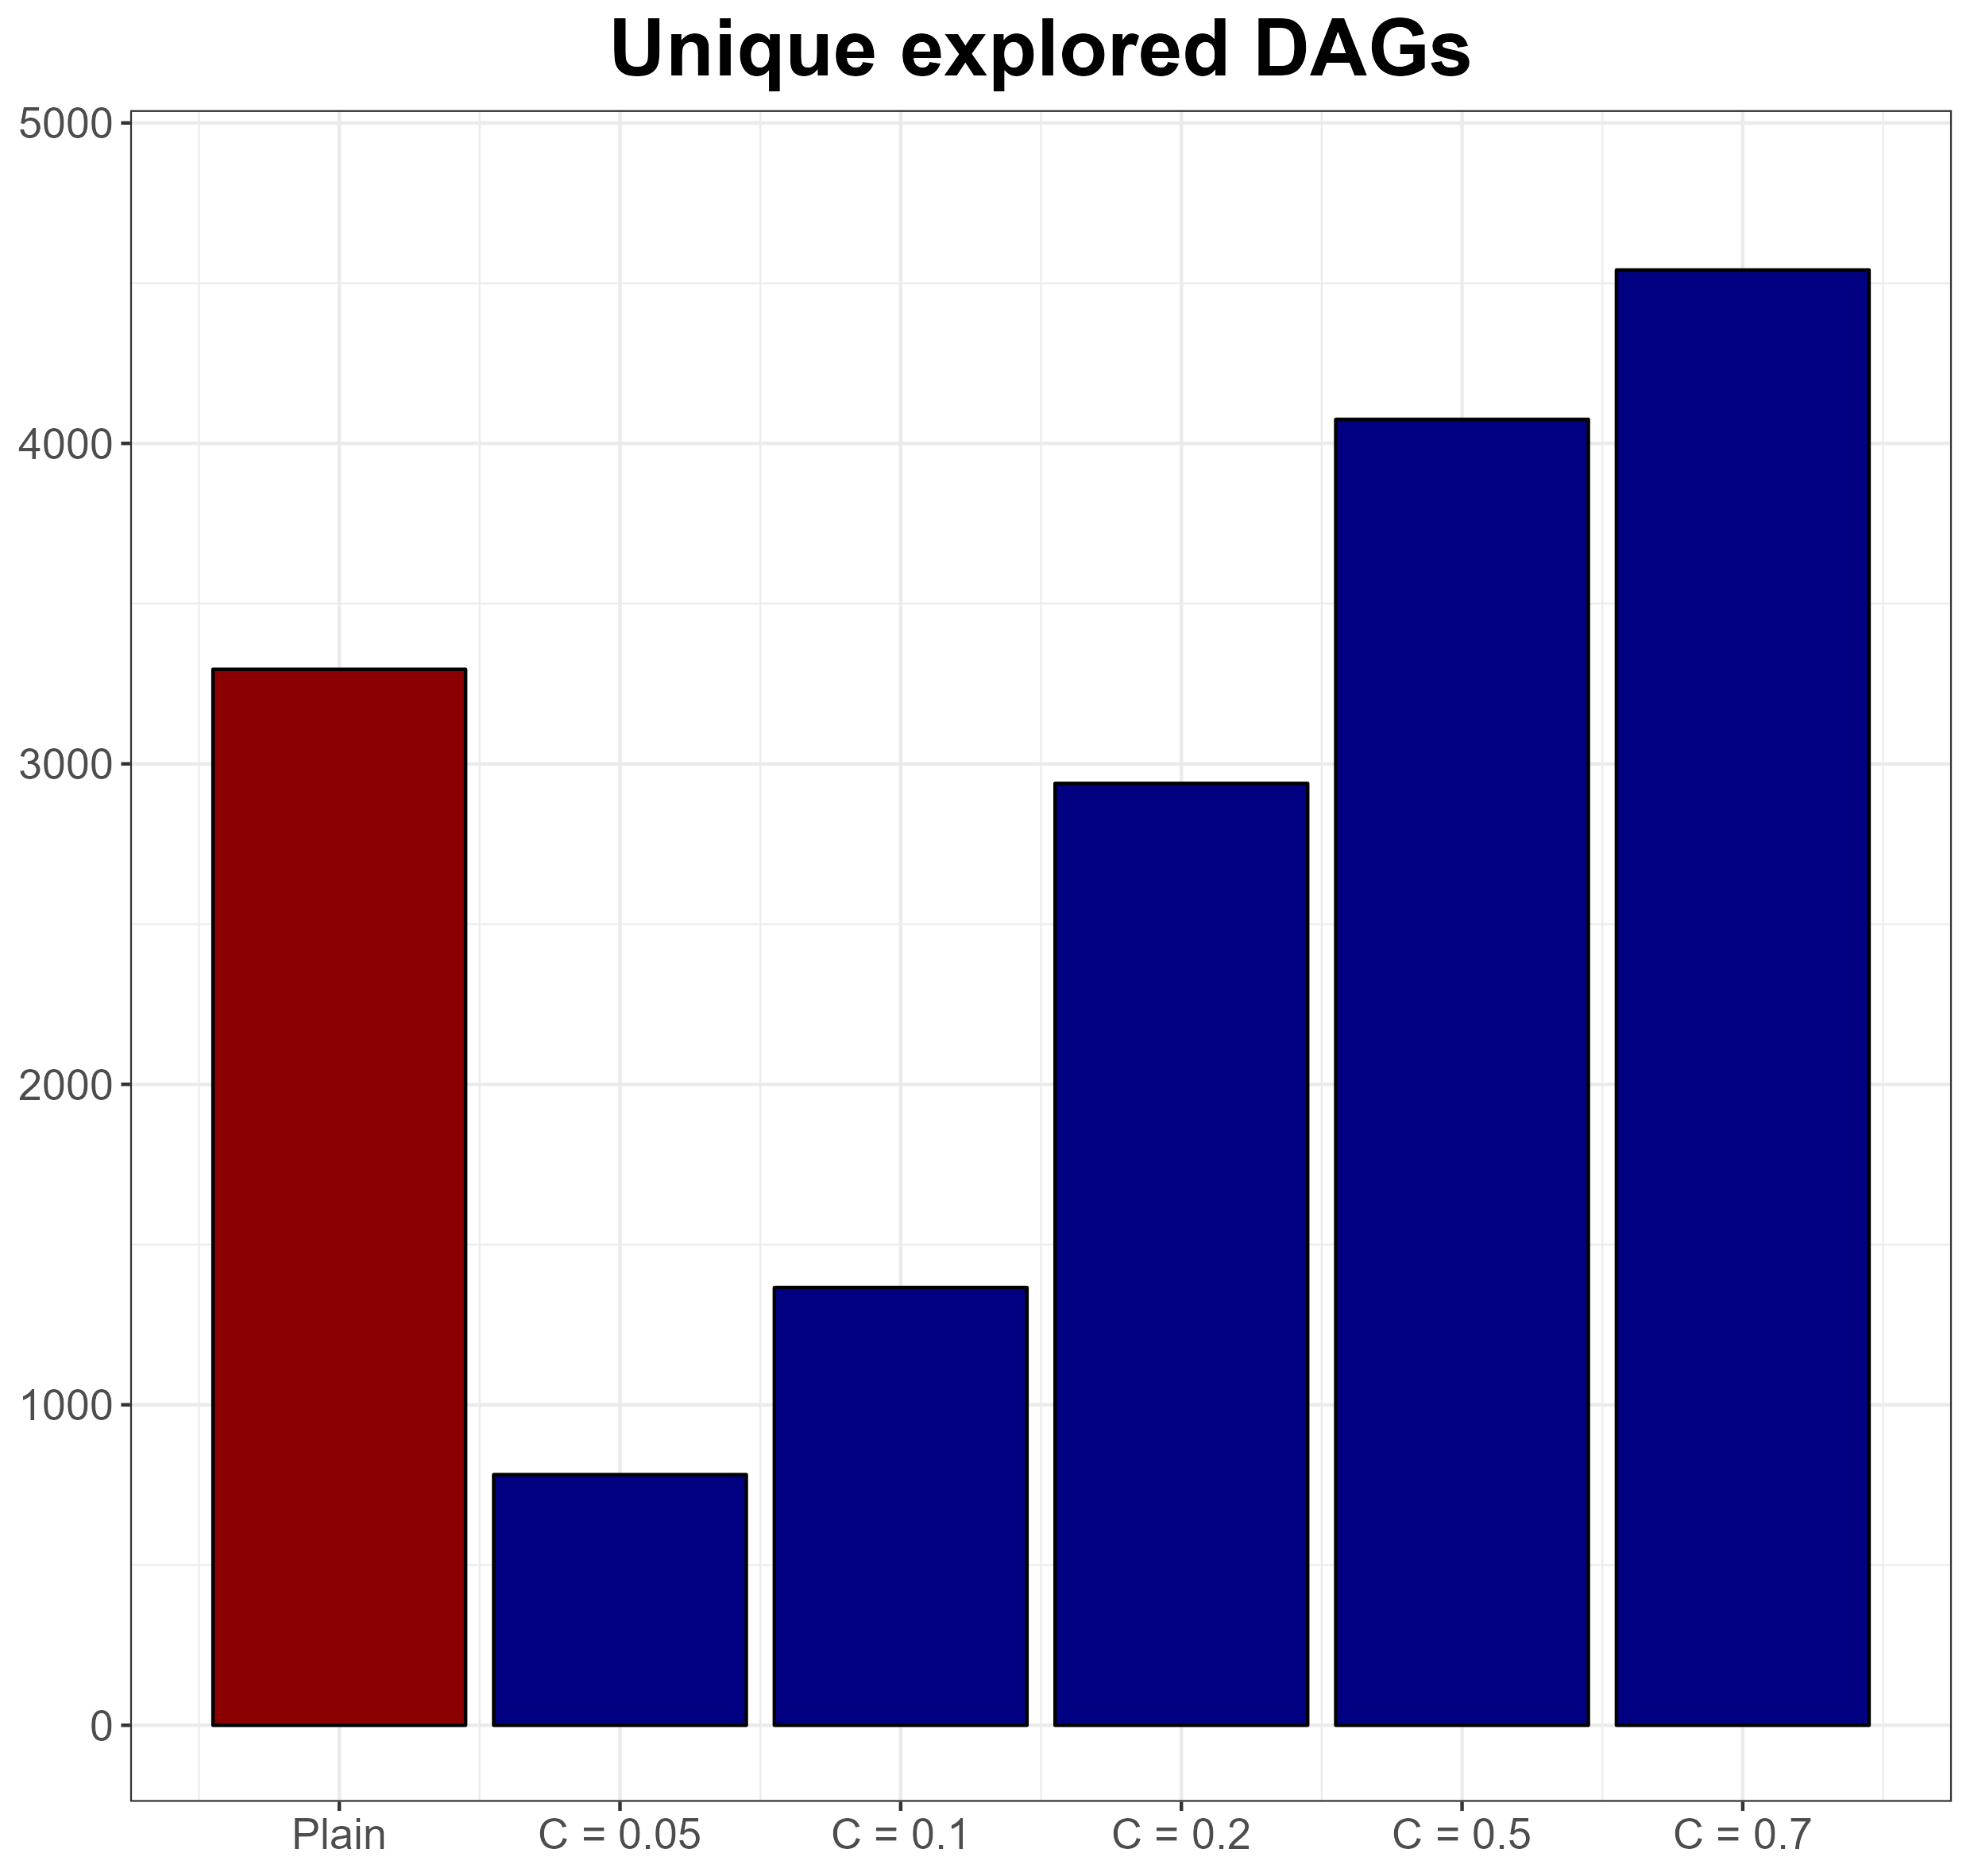
\includegraphics[width=0.3\textwidth]{Figures/Adaptive_behaviour/UniqueHist.png}
	\caption{Frequency of unique graph configurations explored by the algorithm across different C levels, with blue bars representing the adaptive scheme and red bars indicating the plain Metropolis algorithm for comparison.}
	\label{fig:unique-hist}
\end{figure}

This reasoning is here confirmed in \textit{Figure} \ref{fig:unique-hist}, which displays the number of unique DAGs explored by the algorithm on the y-axis. The data indicate that, as the parameter $C$ increases, the algorithm exhibits an enhanced ability to explore the parameter space. Specifically, starting from $C = 0.5$, the exploration of DAGs surpasses that achieved by the plain Metropolis algorithm. Whether this increased exploration translates into improved convergence to the true posterior will be evaluated in subsequent simulations.

\paragraph{Edge probability heatmaps}

In \textit{Figure} \ref{fig:c-heatmaps}, the final edge probabilities are presented. These probabilities are computed based on the sampled data, reflecting the frequency with which each edge is included in the explored DAGs. They are defined as follows:

\begin{equation} \label{edge-probs}
	\hat{p}_{u \rightarrow v} = \frac{1}{S} \sum_{s = 1}^S \mathbbm{1}_{u \rightarrow v}\{\mathcal{D}^{(s)} \}
\end{equation}

expressing the proportion of times the edge $u \rightarrow v$ appears in the sampled graphs.

\begin{figure}[h] 
	\centering
	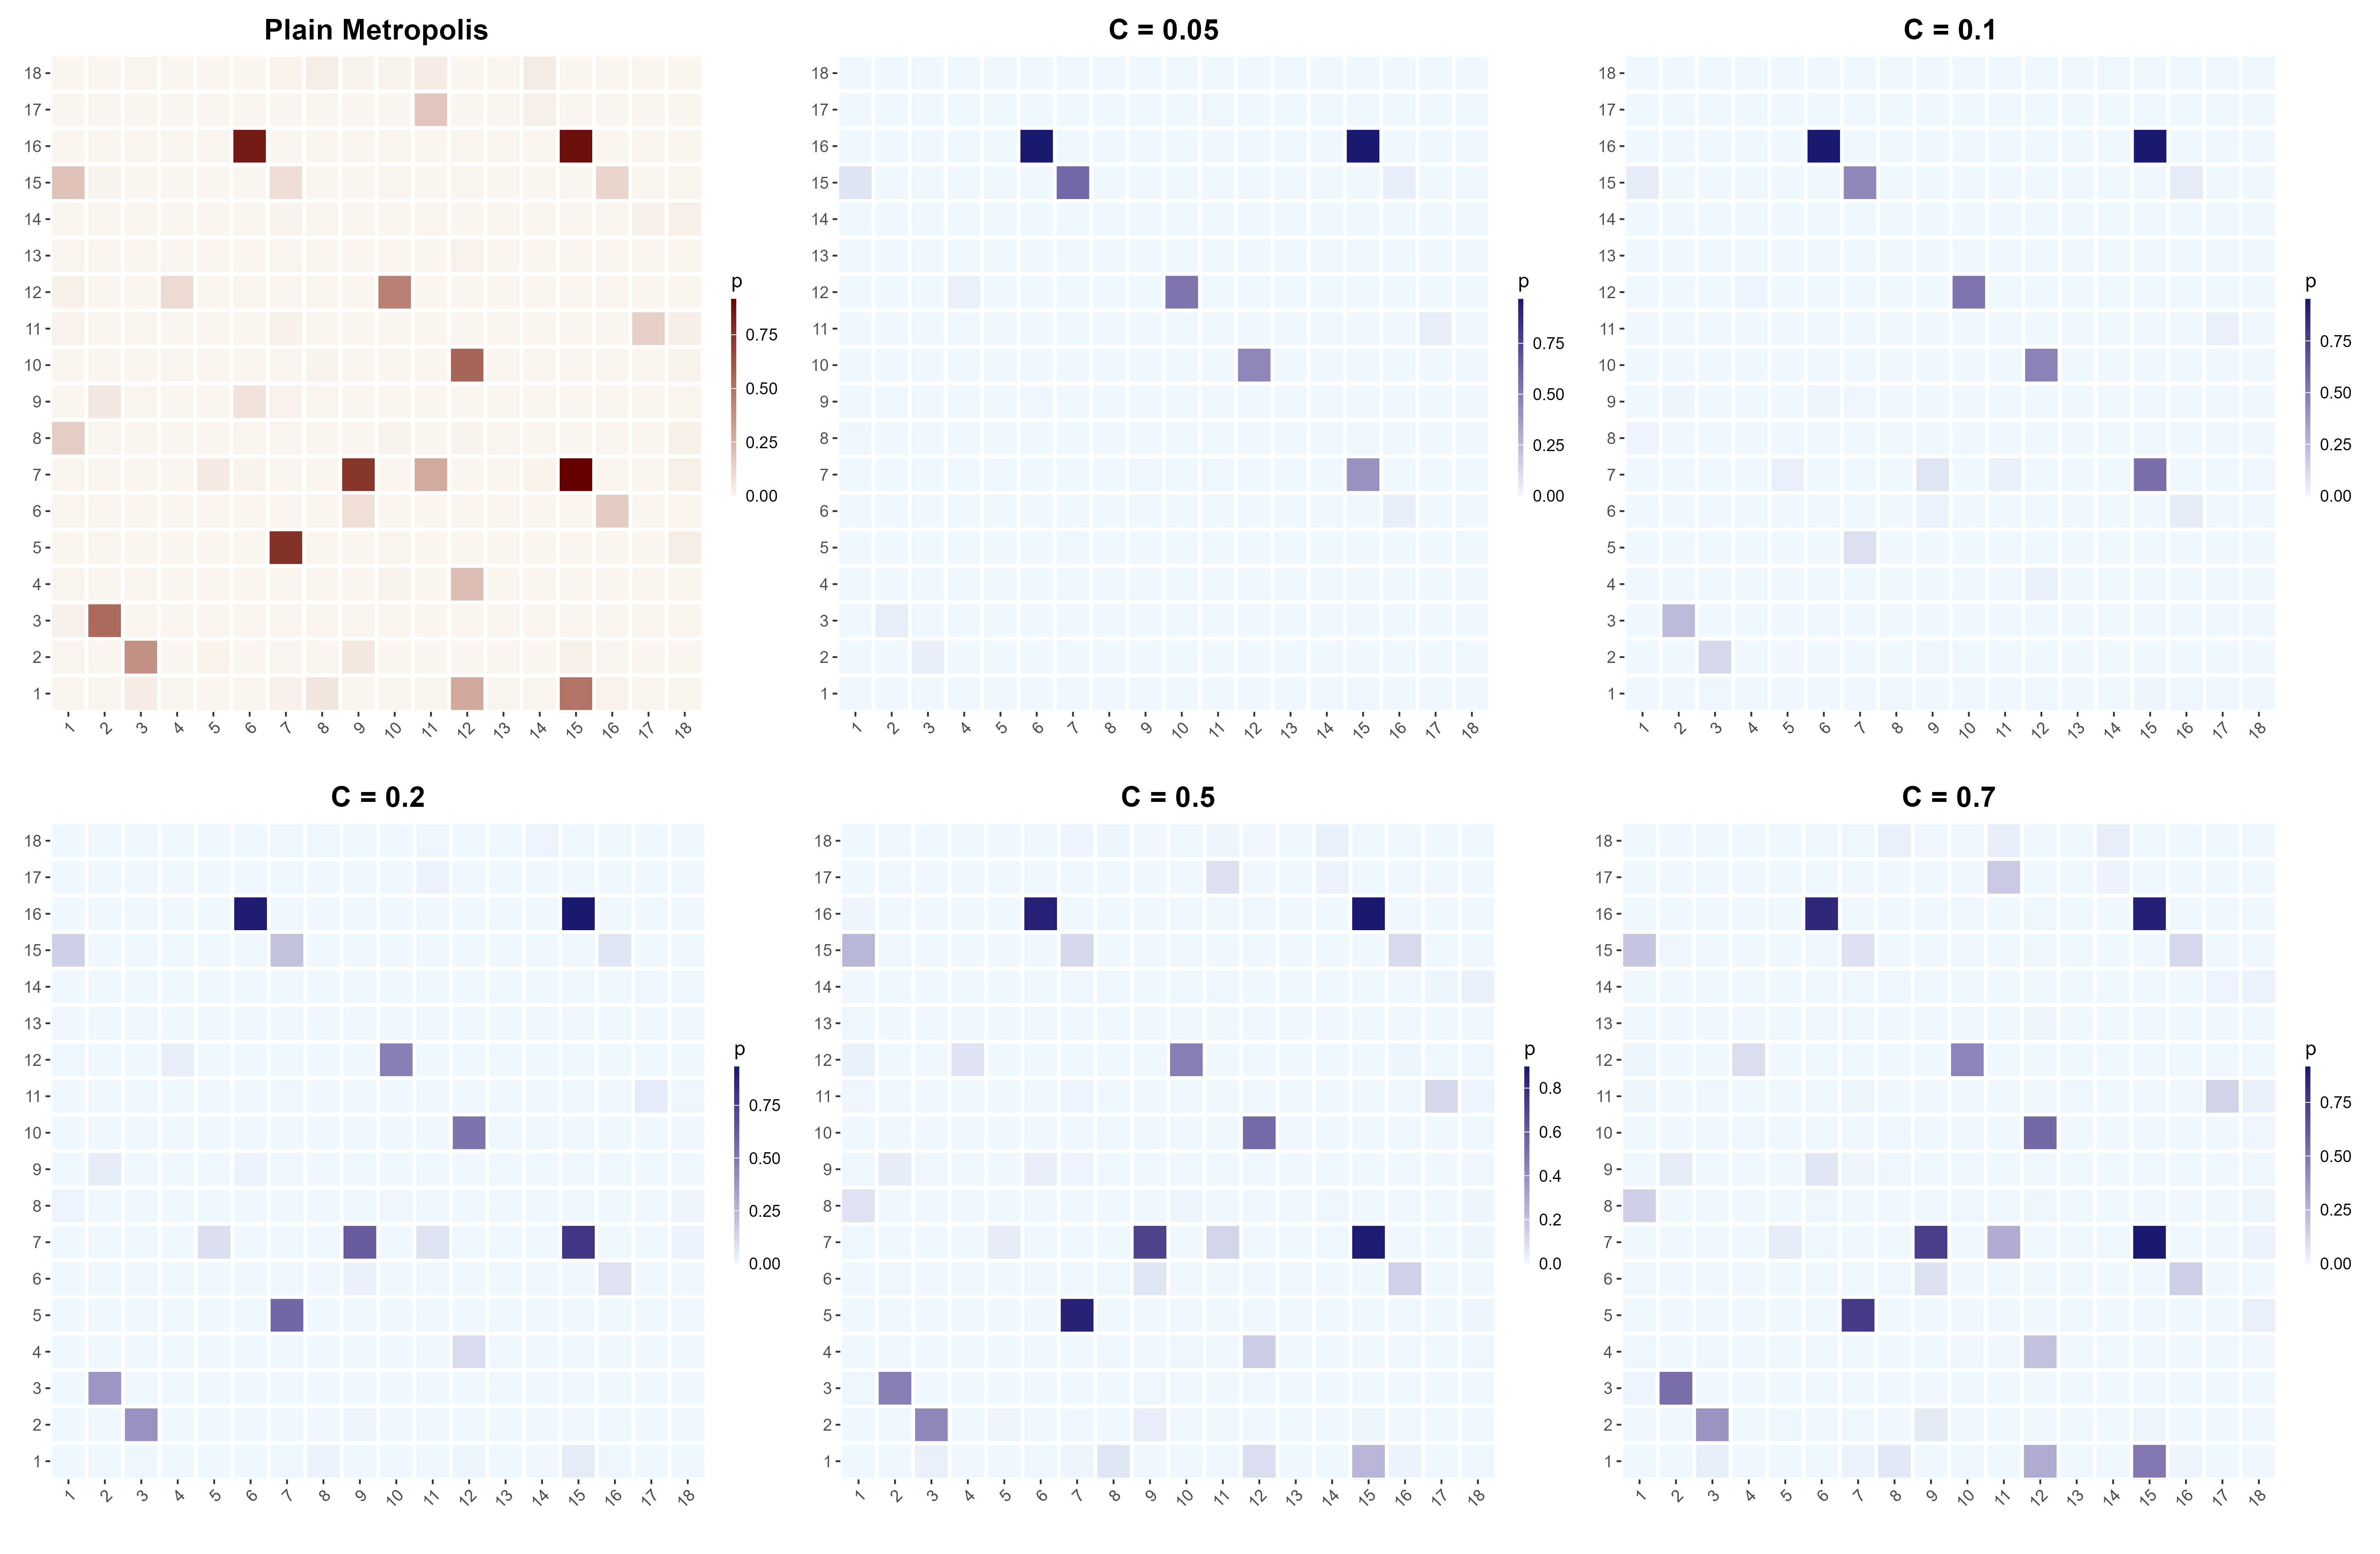
\includegraphics[width=0.9\textwidth]{Figures/Adaptive_behaviour/heatmaps.png}
	\caption{Comparison of edge probability of inclusion between the plain Metropolis algorithm and its adaptive counterpart (depicted in blue) as the parameter C increases.}
	\label{fig:c-heatmaps}
\end{figure}

The results indicate that setting the parameter $C=0.7$ leads to insufficient adaptation, resulting in final probabilities that are nearly identical to those of the standard Metropolis algorithm.  In contrast, values lower than $C=0.5$ trigger overly strong adaptation, limiting the algorithm’s ability to effectively explore the state space. Consequently, $C=0.5$ is chosen for subsequent comparisons as it achieves a better balance between adaptation and exploration.

\paragraph{Convergence analysis}

\begin{figure}[h] 
	\centering
	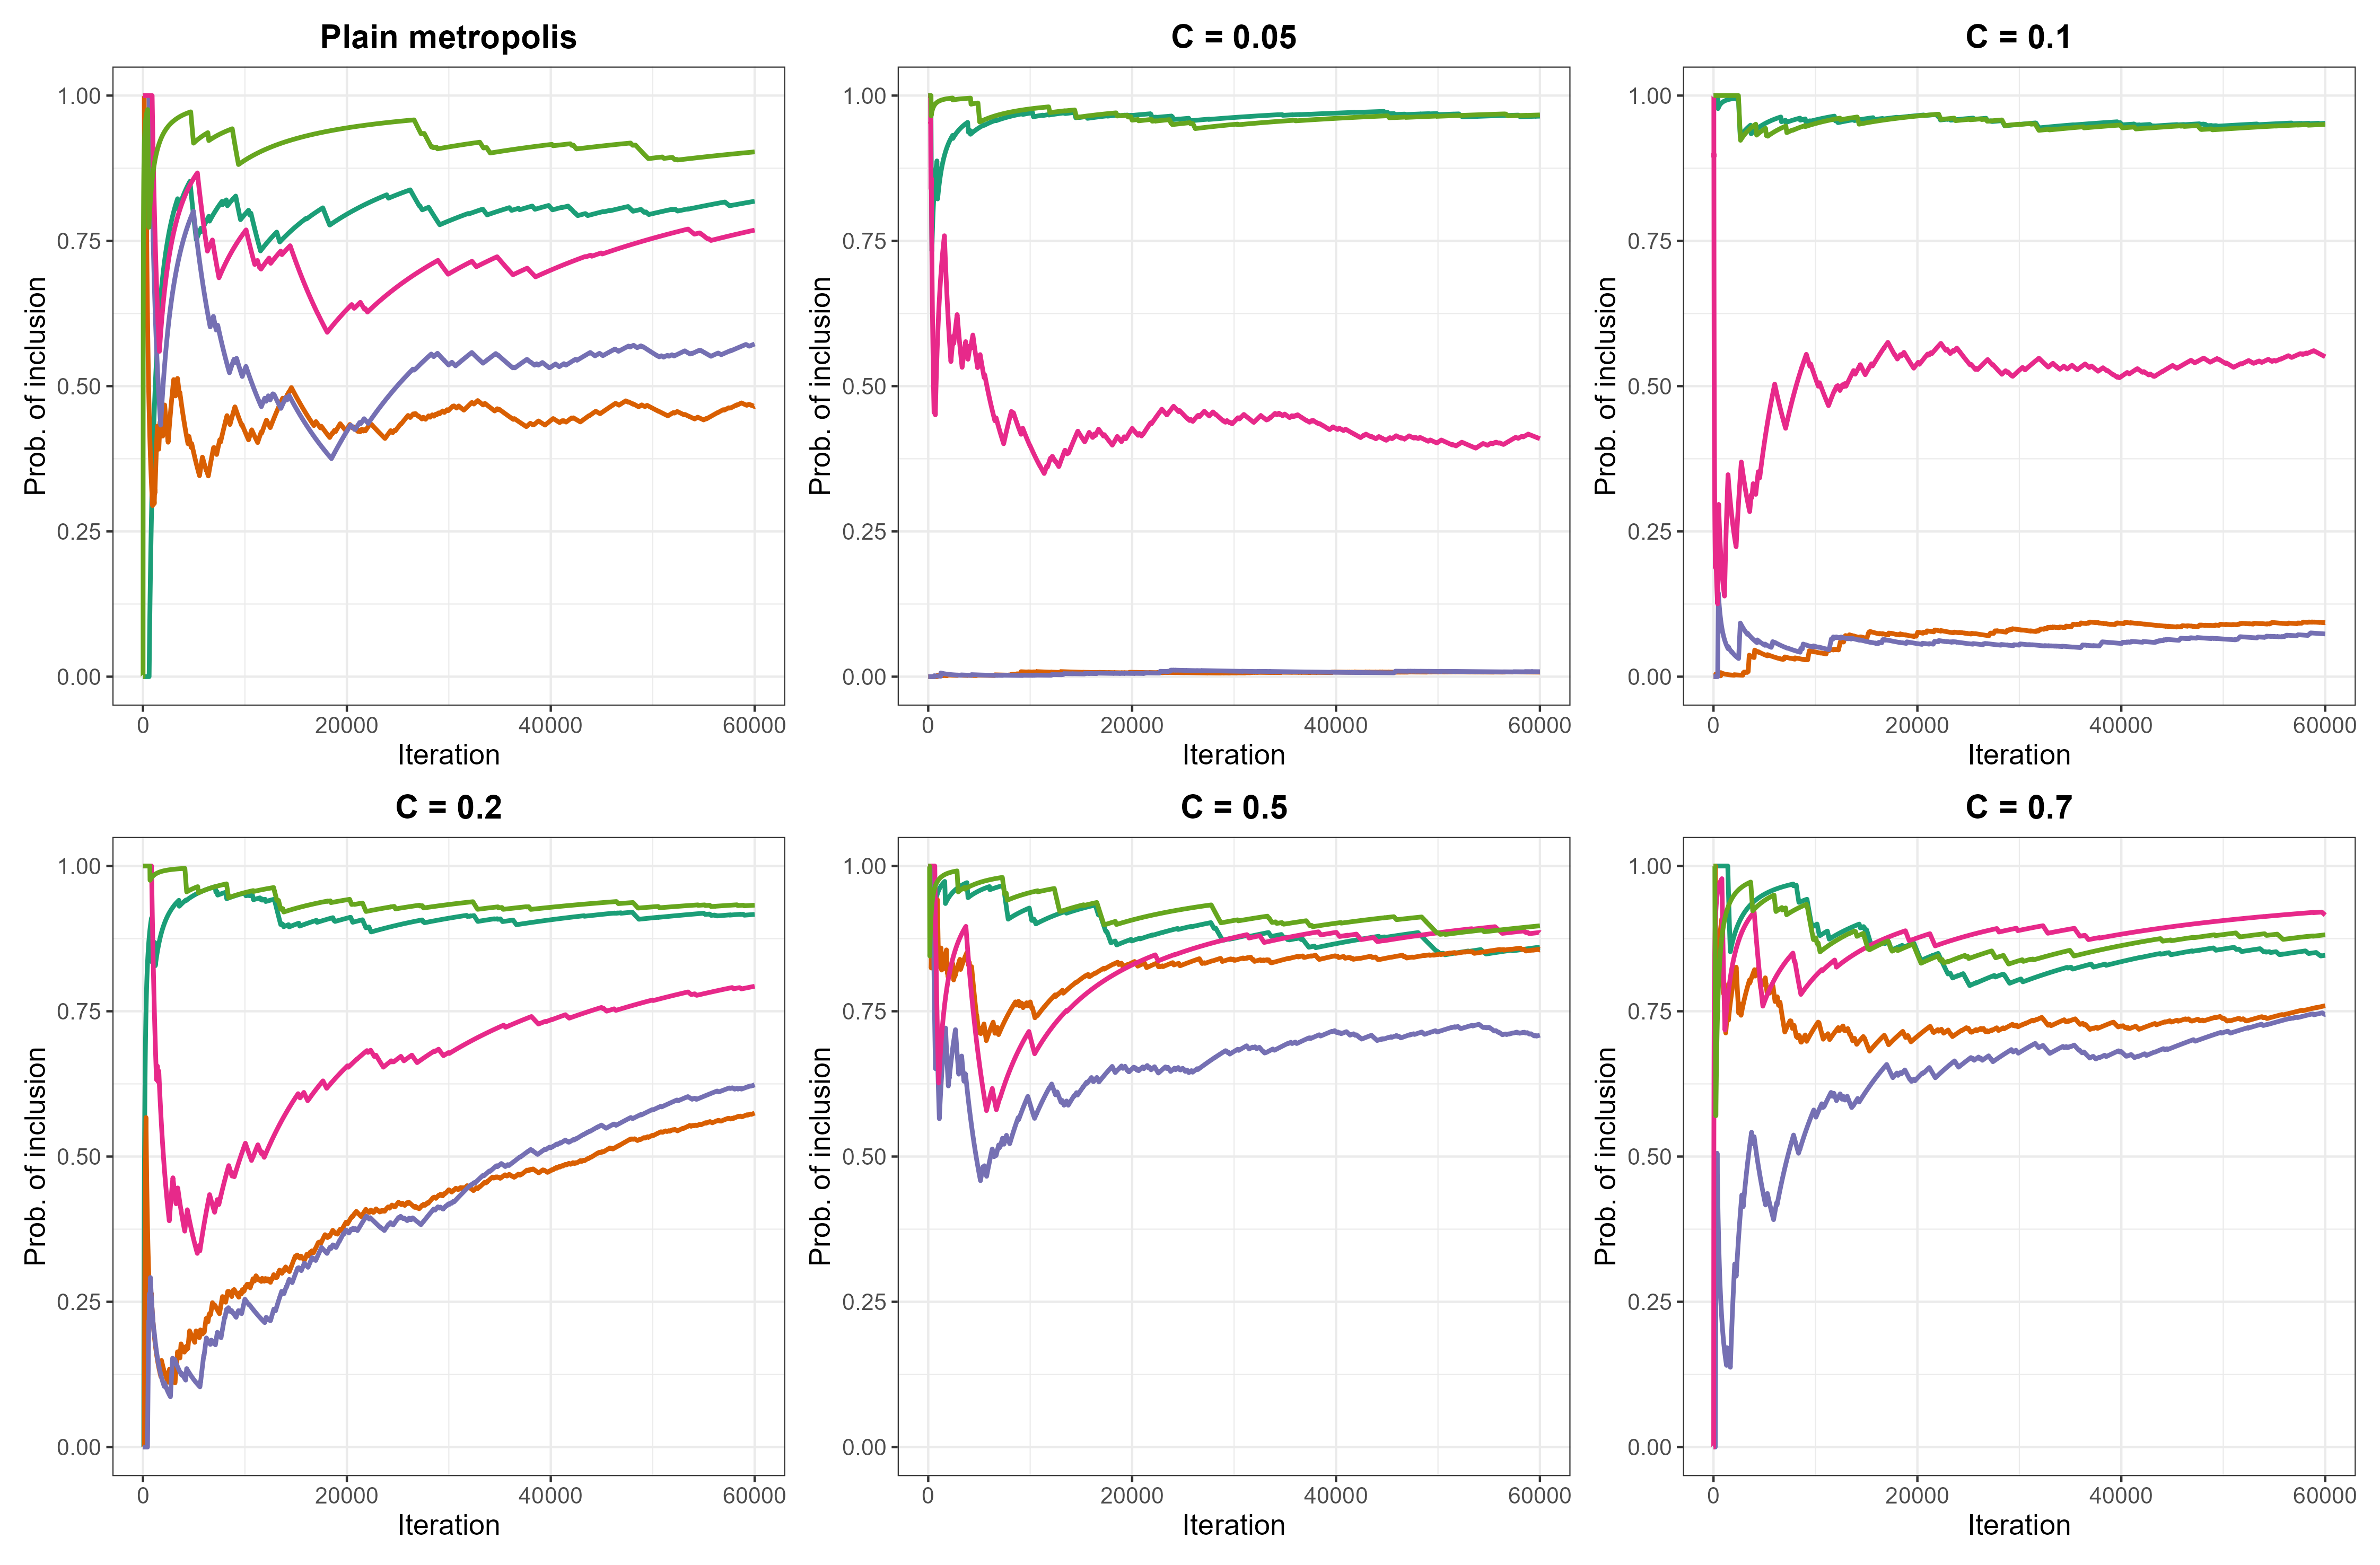
\includegraphics[width=0.9\textwidth]{Figures/Adaptive_behaviour/nodes_trace.png}
	\caption{Cumulative traceplot of edge inclusion probability. Only nodes that exhibit a probabilty higher than 0.5 are included in the Figure.}
	\label{fig:c-convergence}
\end{figure}

As illustrated in \textit{Figure} \ref{fig:c-convergence}, the adaptive MCMC algorithm, particularly at higher values of $C$, demonstrates improved performance in terms of convergence, as indicated by the posterior probabilities reaching higher values. However, to fully assess whether this improvement translates into better overall performance, further simulations will be necessary. It is worth noting that while the exploration of the parameter space appears similar to that of the traditional Metropolis algorithm, indicating a reduced risk of bias from limited space exploration, a comprehensive evaluation is needed to confirm these initial observations.

\section{Birth Death MCMC Model}

\subsection{Theoretical Background}

In the context of evaluating changes to a DAG structure, the death ratio $\delta_e(D,L)$ is defined as:

$$
\delta_e (D,L) = min \  \Bigg\{ \frac{P(\mathcal{D}^{-e},D^{-e},L^{-e} \ | \ X)}{P(\mathcal{D},D,L \ | \ X)} \ ,1 \ \Bigg\} 
$$

To compute $\delta_e(D,L)$, the key objective is to derive the ratio:

$$
\frac{P(\mathcal{D}^{-e},D^{-e},L^{-e} \ | \ X)}{P(\mathcal{D},D,L \ | \ X)}
$$

This ratio compares the posterior probabilities of the DAG before and after the removal of an edge $e$. To facilitate this computation, consider the relationship:

$$
P(\mathcal{D},D,L \ | \ X) = \frac{P(\mathcal{D},D,L,X)}{P(X)}
$$

and the factorization:

$$
P(\mathcal{D},D,L,X) = P(X,D,L \ |\mathcal{D})P(\mathcal{D})
$$

Substituting these into the expression for the ratio, we obtain:

$$
\frac{P(\mathcal{D}^{-e},D^{-e},L^{-e} \ | \ X)}{P(\mathcal{D},D,L \ | \ X)} = \frac{P(X ,D^{-e},L^{-e} \ | \ \mathcal{D}^{-e})}{P(X,D,L \ | \ \mathcal{D})}\  \times \frac{P(\mathcal{D}^{-e})}{P(\mathcal{D})}\ \times \frac{P(X)}{P(X)} 
$$

Here, the ratio $\frac{P(X)}{P(X)}$  simplifies to 1, reducing the expression to:

$$
\frac{P(\mathcal{D}^{-e},D^{-e},L^{-e} \ | \ X)}{P(\mathcal{D},D,L \ | \ X)} = \frac{P(X ,D^{-e},L^{-e} \ | \ \mathcal{D}^{-e})}{P(X,D,L \ | \ \mathcal{D})}\  \times \frac{P(\mathcal{D}^{-e})}{P(\mathcal{D})}\ 
$$

The prior probability $P(\mathcal{D})$ is associated with the structure of the DAG $\mathcal{D}$. For each DAG $\mathcal{D}$, a prior probability is assigned to its adjacency matrix $A^{\mathcal{D}}$, which is a symmetric 0-1 matrix representing the skeleton of $\mathcal{D}$. A Bernoulli prior is independently assigned to each element in the lower triangular part of the adjacency matrix, resulting in the following expression for the prior probability:

$$
P(A^\mathcal{D})=\pi^{|A^\mathcal{D}|}(1- \pi)^{\frac{q(q-1)}{2}-|A^\mathcal{D}|}
$$
Consequently, the following relationship holds: $P(\mathcal{D}) \propto P(A^{\mathcal{D}})$.

More specifically, when considering operations such as inserting, deleting, or reversing an edge, it is sufficient to compare the priors associated with these specific changes. For instance, if the prior probability that adding a new edge is 0.6, the corresponding odds for adding the edge are 1.5, calculated as the ratio of the probability of adding the edge to the probability of not adding it (i.e., $\frac{0.6}{0.4}$). Similarly, the odds for deleting an edge, given the prior probability of 0.4 for this operation, are 0.666 ($\frac{0.4}{0.6}$). For the reverse operation, assuming neutral prior probabilities, the odds are 1.

Next, consider the term $P(X ,D^{-e},L^{-e} \ | \ \mathcal{D}^{-e})$. Suppose an edge $(h,j)$  has been removed. Then, this probability can be expressed as:

$$
P(X,D \  \backslash D_{jj}, L\ \backslash L_{\prec j ]} \ | \ \mathcal{D} )
$$

Where $D_{jj}$ is the diagonal element whereas $L_{\prec j ]}$ is the column of coefficients associated to node $j$. 

This expression is equivalent to the likelihood of all nodes except $j$, plus an integral. The first part simplifies within the ratio, while the second part corresponds to the node-marginal likelihood. This concept is discussed in detail in in \citet{castelletti2022bcdag}, pag. 12.

Consequently, the ratio becomes:

$$
\frac{P(\mathcal{D}^{-e},D^{-e},L^{-e} \ | \ X)}{P(\mathcal{D},D,L \ | \ X)} = \frac{m(X_j \ | X_{pa_{\mathcal{D}'}(j)},\mathcal{D}')}{m(X_j \ | X_{pa_{\mathcal{D}}(j)},\mathcal{D})}\ \times \ \frac{P(\mathcal{D}^{-e})}{P(\mathcal{D})}
$$

where the last fraction is expressed in terms of odds and $\mathcal{D}^{-e}$ denotes the DAG $\mathcal{D}$ with the edge $e$ removed. The explicit formula for the node-marginal likelihood can be found in \citet{castelletti2022bcdag}, pag. 8 and an alternative formulation is provided in \citet{castelletti2021bayesian} (supp. material, pag. 6).

\subsection{Implementation Code}

The algorithm  begins with an initial DAG and iteratively proposes modifications by either adding or deleting edges between nodes. Each potential change is evaluated for its validity—specifically, whether it preserves the acyclic property of the graph. This validation is critical because the goal is to maintain a DAG structure while exploring various configurations.
For each proposed modification, the algorithm calculates the plausibility of the new graph configuration relative to the existing one. This is done by comparing the marginal likelihoods of the proposed and current graphs, alongside the prior probabilities of edge inclusion or exclusion. The use of prior ratios helps incorporate existing knowledge about the structure of the graph, influencing which modifications are more likely to be accepted. The resulting probabilities are then adjusted using a softmax function, which transforms the raw likelihoods into a probability distribution that favors more promising moves.
Moreover, the algorithm tracks waiting times associated with each proposed move, which reflects the efficiency of the sampling process. 

\begin{algorithm}[H]
	\caption{Bith-Death MCMC algorithm}
	\begin{algorithmic}[1]
		\State \textbf{Initialize} $G$, $D$, $L$ and the vector of waiting times
		
		\While{the maximum number of iterations has not been reached}
		\State \textbf{Store} the current DAG configuration
		\State \textbf{Identify} all possible local operations on the current DAG
		\For{each possible operation}
		\If{applying the operation results in a valid DAG}
		\State \textbf{Calculate} the marginal likelihood of the new DAG
		\State \textbf{Store} the birth and death ratio for comparison
		\EndIf
		\EndFor
		\State \textbf{Select} an operation based on calculated probabilities
		\EndWhile
		
		\State \textbf{Return} the final DAG configuration, dag sequence, waiting times, parameters L and D
		\State \textbf{End} birth\_death function
		
	\end{algorithmic}
\end{algorithm}


\section{Diagnostic Techniques for MCMC}

\subsection{Simulation Procedures}

To evaluate the performance of the two algorithms, a series of simulations were carried out. Specifically, 15 simulations were conducted for the Metropolism, Adaptive (with parameters C equal to 0.5) and the BDMCMC algorithm. \textit{Figure} \ref{fig:heat-true} illustrates the true DAG structure used for parameter sampling. The code utilized to generate the data is as follows:

\begin{lstlisting}[language=R]
	q = nrow(DAG)
	w = w
	outDL = rDAGWishart(n = 1, DAG = DAG, a = q, U = diag(1, q))
	L = outDL$L; D = outDL$D
	Sigma = solve(t(L))%*%D%*%solve(L)
	X = mvtnorm::rmvnorm(n = n, sigma = Sigma)
	X <- scale(X, scale = FALSE)
\end{lstlisting}

To simplify the analysis, the true DAG ($\textit{Figure}$ \ref{fig:heat-true}) is selected to be the sole representative within its Markov equivalence class. This choice ensures that the algorithm focuses on a specific DAG configuration, which facilitates the interpretation of the results; in fact, it will be sufficient to assess how well the algorithms perform in identifying this particular structure.

\begin{figure}[h] 
	\centering
	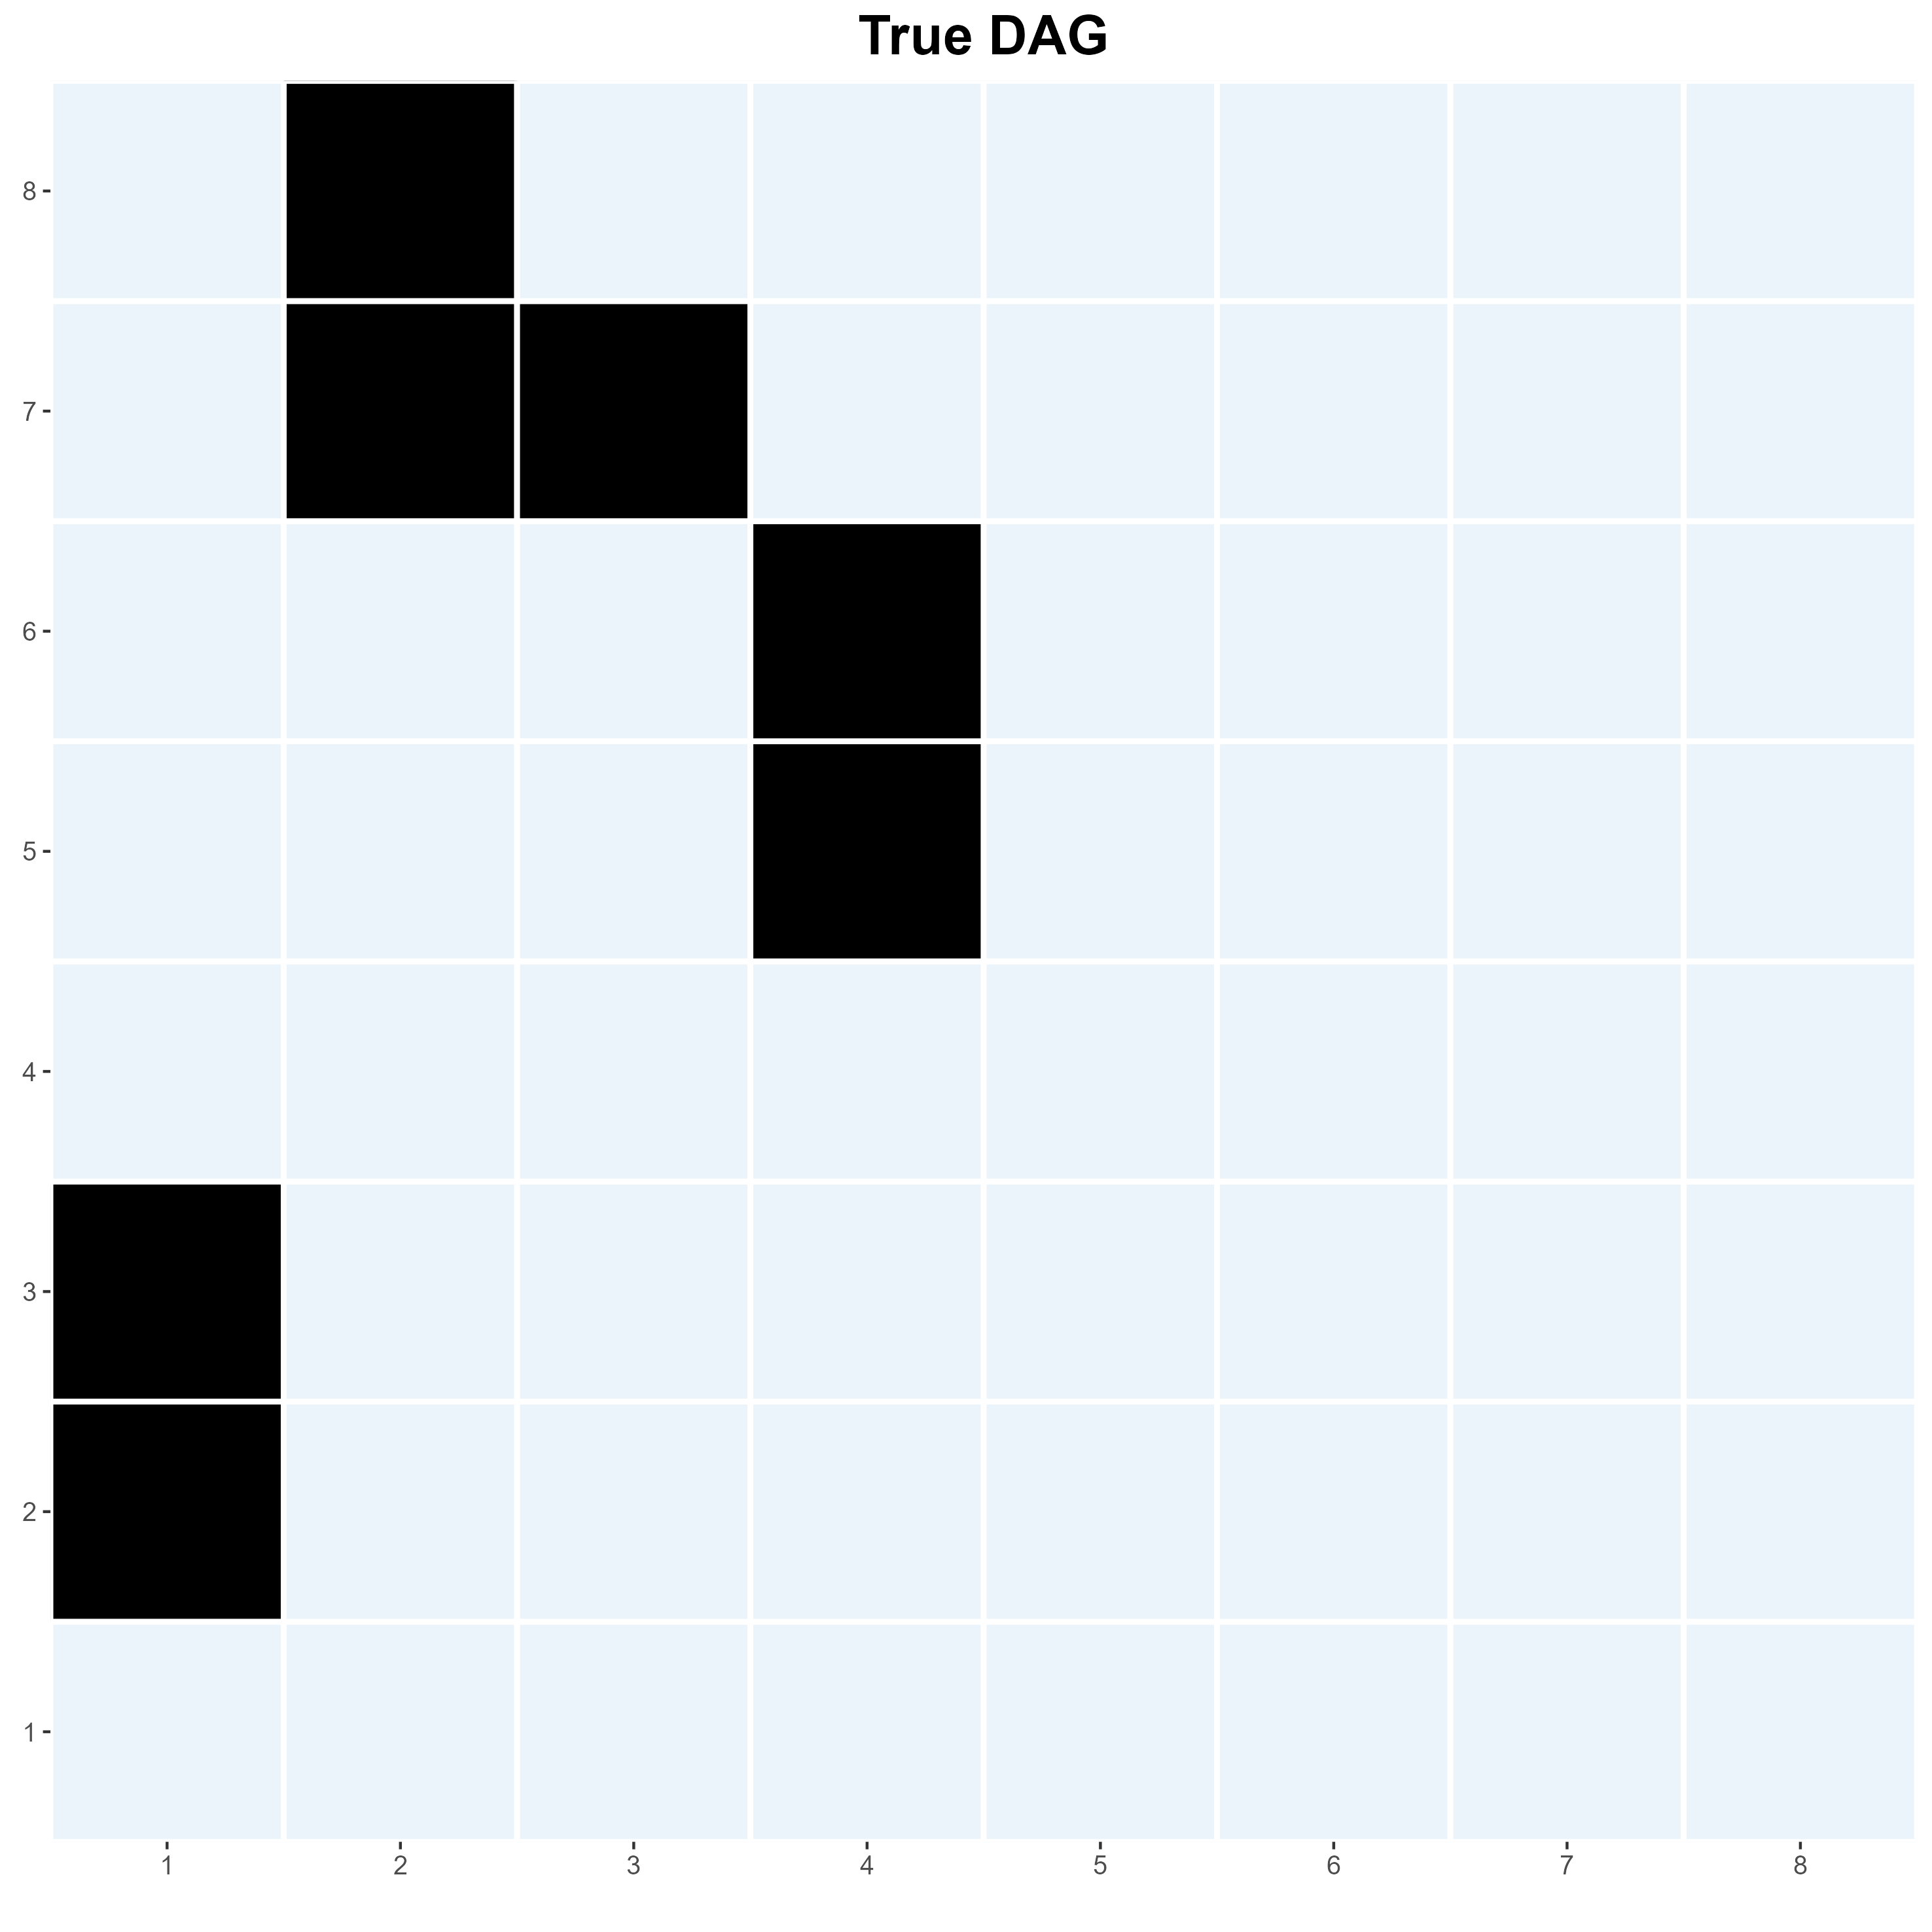
\includegraphics[width=0.3\textwidth]{Figures/Overall_comparison/heat_true.png}
	\caption{Heatmap representing the true dag structure.}
	\label{fig:heat-true}
\end{figure}

In this context, convergence diagnostics for MCMC simulations are crucial for ensuring that the chains have adequately explored the parameter space, yielding reliable and valid estimates of the posterior distribution. Various statistics and diagnostic tools are employed, including the Kolmogorov-Smirnov statistic, Hellinger distances, and complexity measures.
However, one of the challenges of using MCMC-based model determination methods is the difficulty in monitoring convergence. To address this issue, it is essential to identify a parameter that uniquely defines the current model, which will help in achieving more consistent convergence monitoring. Such a parameter would serve as a concise summary of the model’s state, allowing   to track transitions and detect whether the chains are stabilizing.(\citet{brooks2003nonparametric}).

\subsection{Rejection Rates and Graph Sampling}

As illustrated in \textit{Figure} \ref{fig:rejections}, the standard Metropolis algorithm exhibits a notably higher rejection rate during the acceptance-rejection process, with a significant number of outliers detected; some exceeding 1,500 consecutive rejections. This elevated rejection rate arises from the algorithm's strategy of proposing new DAGs by randomly selecting configurations from a uniform distribution among the nearest possible DAGs. This approach does not consider the likelihood or suitability of these configurations based on the data, leading to frequent selection of DAGs that are poorly aligned with the underlying structure of the problem.
In contrast, the adaptive scheme, which refines the proposal distribution by incorporating information from previously accepted DAGs, more effectively targets configurations that are consistent with the data. This targeted approach reduces the number of rejections, as the algorithm is better equipped to propose DAGs that are more likely to be accepted, thereby improving the overall efficiency of the sampling process.

\begin{figure}[h] 
	\centering
	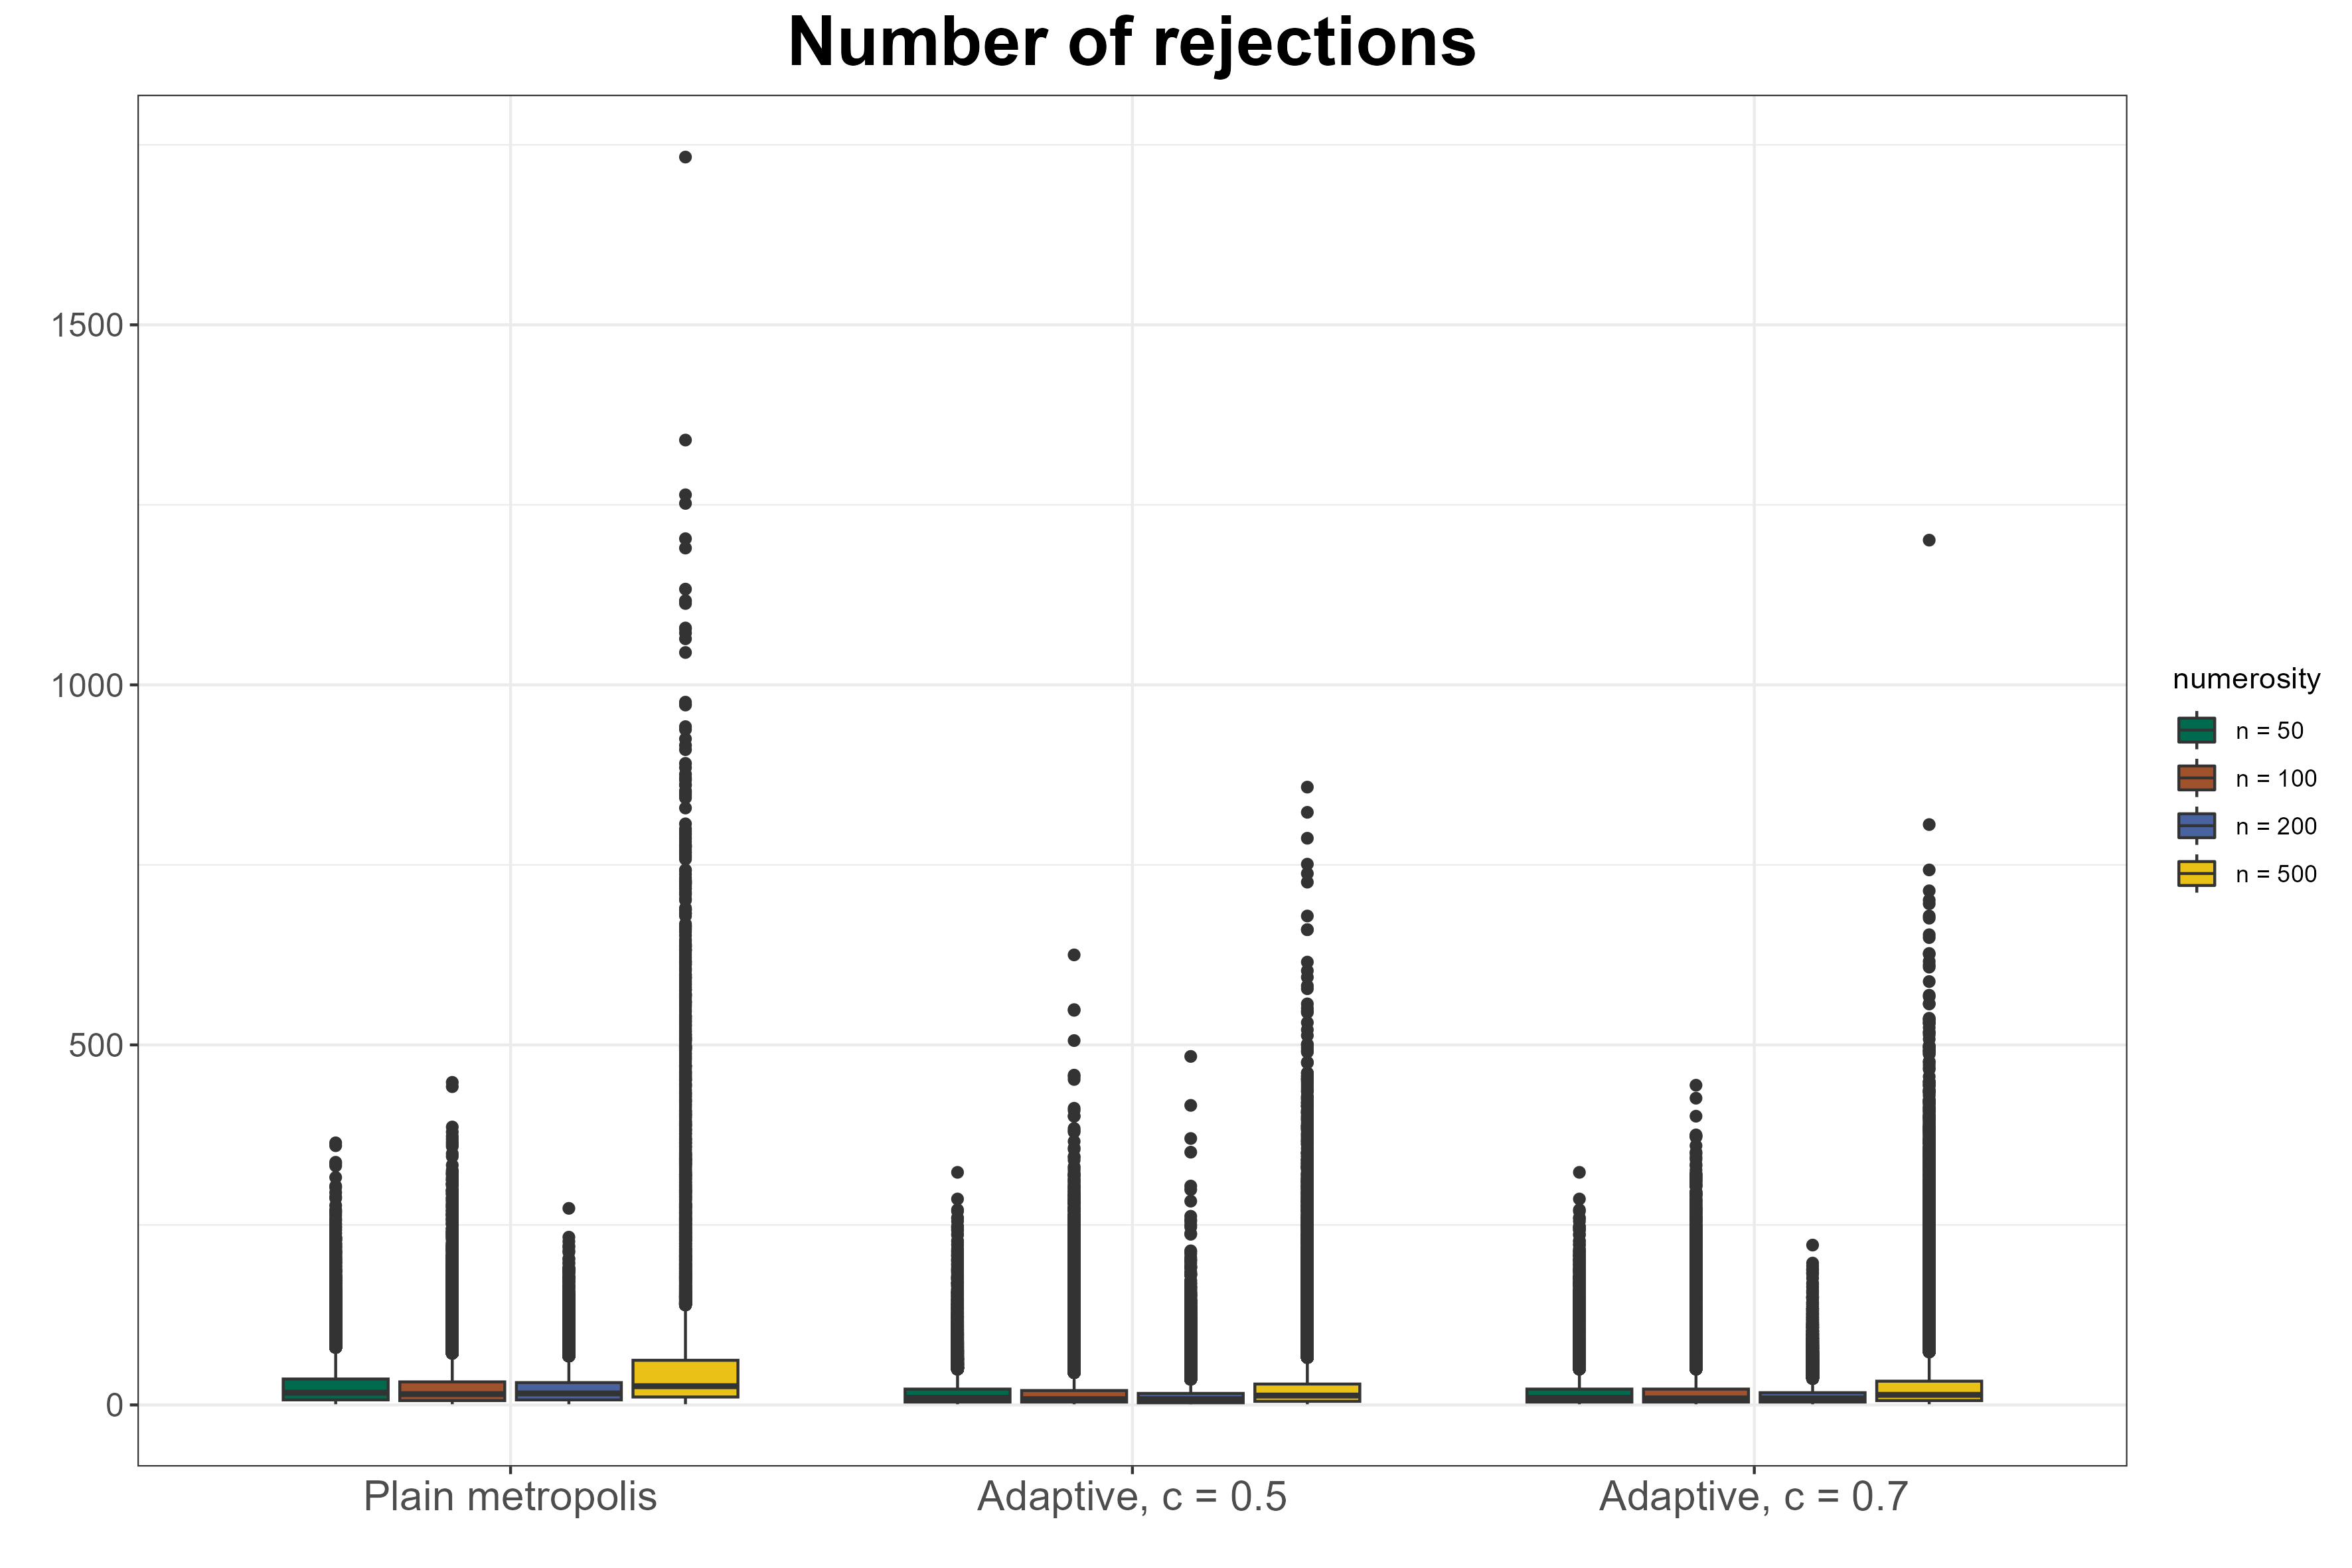
\includegraphics[width=0.65\textwidth]{Figures/Overall_comparison/Boxplot_rejected.png}
	\caption{Number of rejections across algorithm and sample size.}
	\label{fig:rejections}
\end{figure}

\subsection{Complexity Analysis}

In \textit{Figure} \ref{fig:box-visit-graphs}, the distribution of the number of visited graphs across different numerosities is presented. It can be observed that for lower numerosities, the plain Metropolis algorithm results in broader exploration of the state space. However, as numerosity increases, the birth-and-death (BD) algorithm begins to outperform the Metropolis approach in terms of the number of distinct graphs visited. This shift may be related to the differing proposal mechanisms of the two algorithms.

The plain Metropolis algorithm bases its moves on the acceptance or rejection of proposals determined by the ratio of marginal likelihoods and prior probabilities. When numerosity is low, this simple mechanism could lead to quicker exploration, as the algorithm easily navigates the space of potential graph configurations. However, with higher numerosity, the BD algorithm—by considering all possible local moves and sampling them with probabilities proportional to their likelihood—may better adapt to the additional data. 

\begin{figure}[h] 
	\centering
	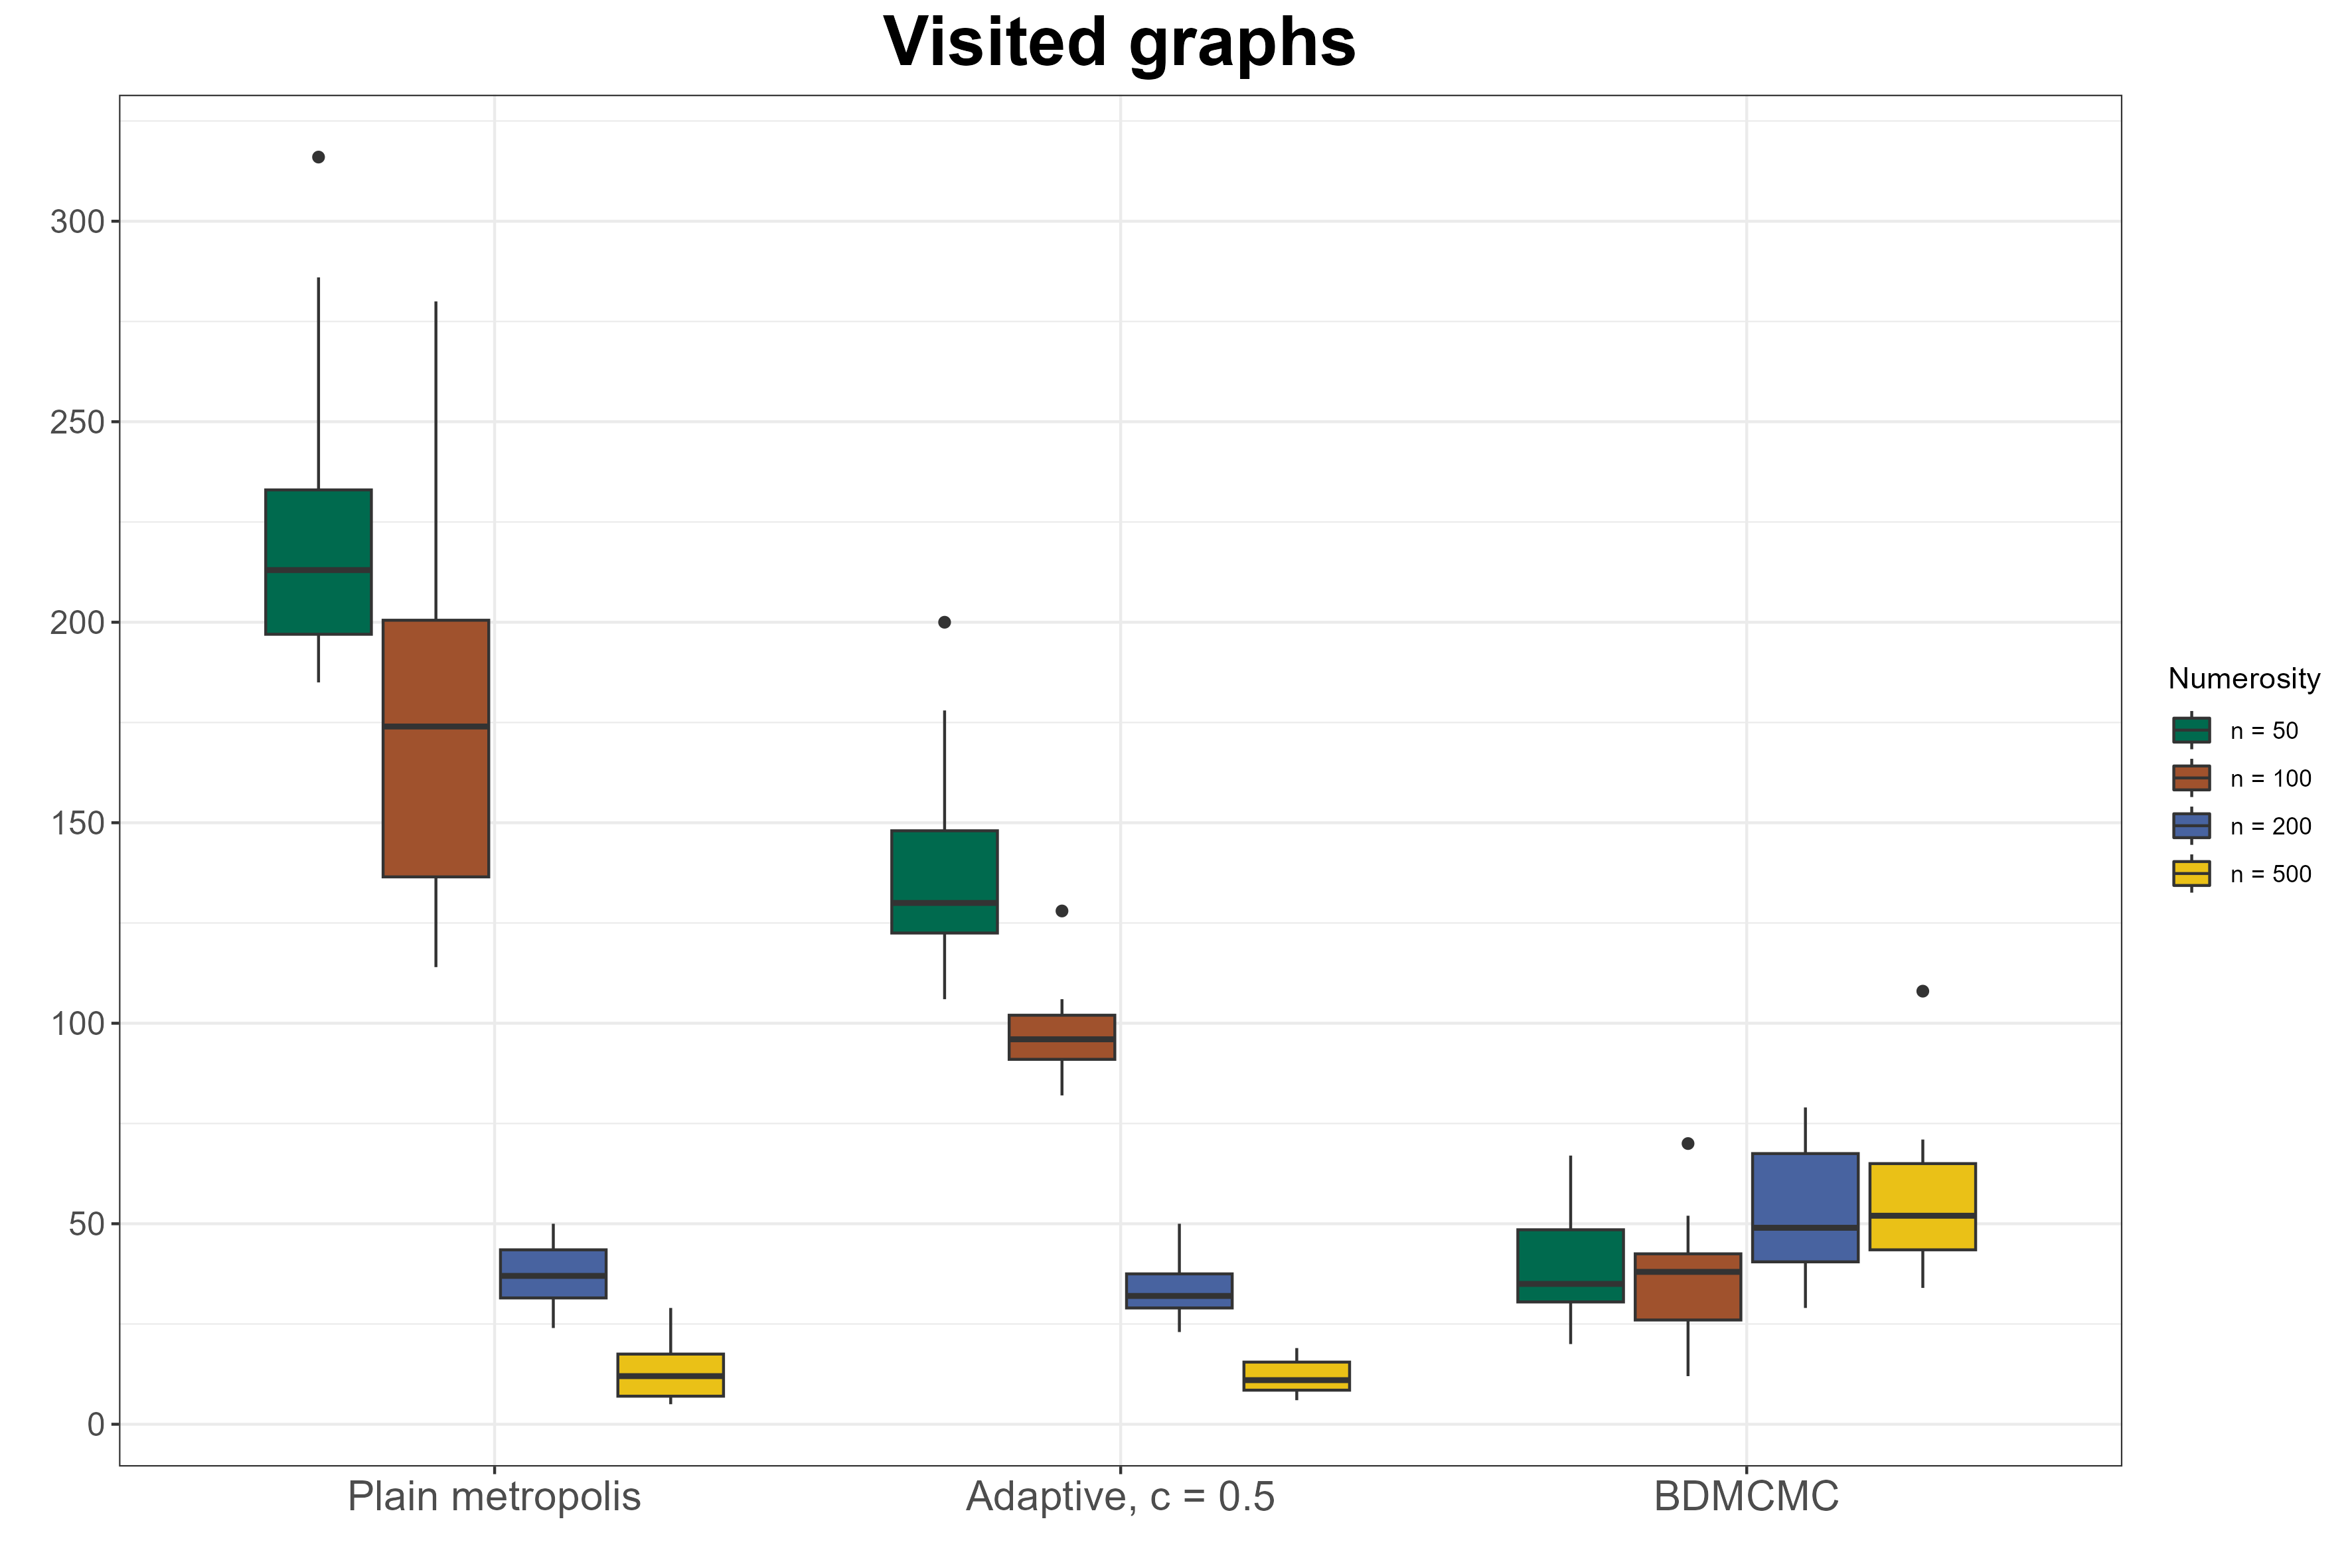
\includegraphics[width=0.6\textwidth]{Figures/Diagnostic/Boxplot_visit_graphs_org.png}
	\caption{Unique visited graph structures by the three tested algorithms across sample size.}
	\label{fig:box-visit-graphs}
\end{figure}

Moreover, it is worth noting that there are no overlapping graph configurations across different chain replicates. This is primarily due to the immense size of the graph space, which grows exponentially with the number of parameters. Specifically, for a system with $p$ nodes, the number of possible DAG configurations scales as $2^{\frac{p(p-1)}{2}}$. As $p$ increases, this exponential growth leads to a vast model space, making it highly unlikely for different chain replicates to explore the same graph configurations. \hfill \break

There are two primary distributions of interest, the number of edges and the model probabilities. First, the distribution of the number of edges is considered which can be thought of as measure of model complexity.
The complexity of a DAG refers to the number of edges (or "1s") in the adjacency matrix representing the graph. This measure helps quantify the structural richness of the sampled graphs over iterations. For binary matrices, the complexity is straightforward, as it counts the occurrences of 1s. This measure is useful because it allows us to assess whether different chains explore similar structural regions of the parameter space. A lack of variability in complexity over chains might indicate poor mixing, while high variability suggests better exploration of different potential models.  Formally, for a DAG adjacency matrix $\mathcal{D}$, the complexity $C(\mathcal{D})$ is defined as:

$$
C(\mathcal{D}) = \sum_{i,j} \mathcal{D}_{i,j}
$$

where $\mathcal{D}_{i,j}$ is the element of the adjacency matrix corresponding to the edge from node $i$ to node $j$.

\begin{figure}[!ht]
	\centering
	\resizebox{\textwidth}{6.5cm}{  
		\begin{minipage}{\textwidth}
			\centering
			
			% First figure
			\begin{subfigure}[b]{0.45\textwidth}   
				\centering
				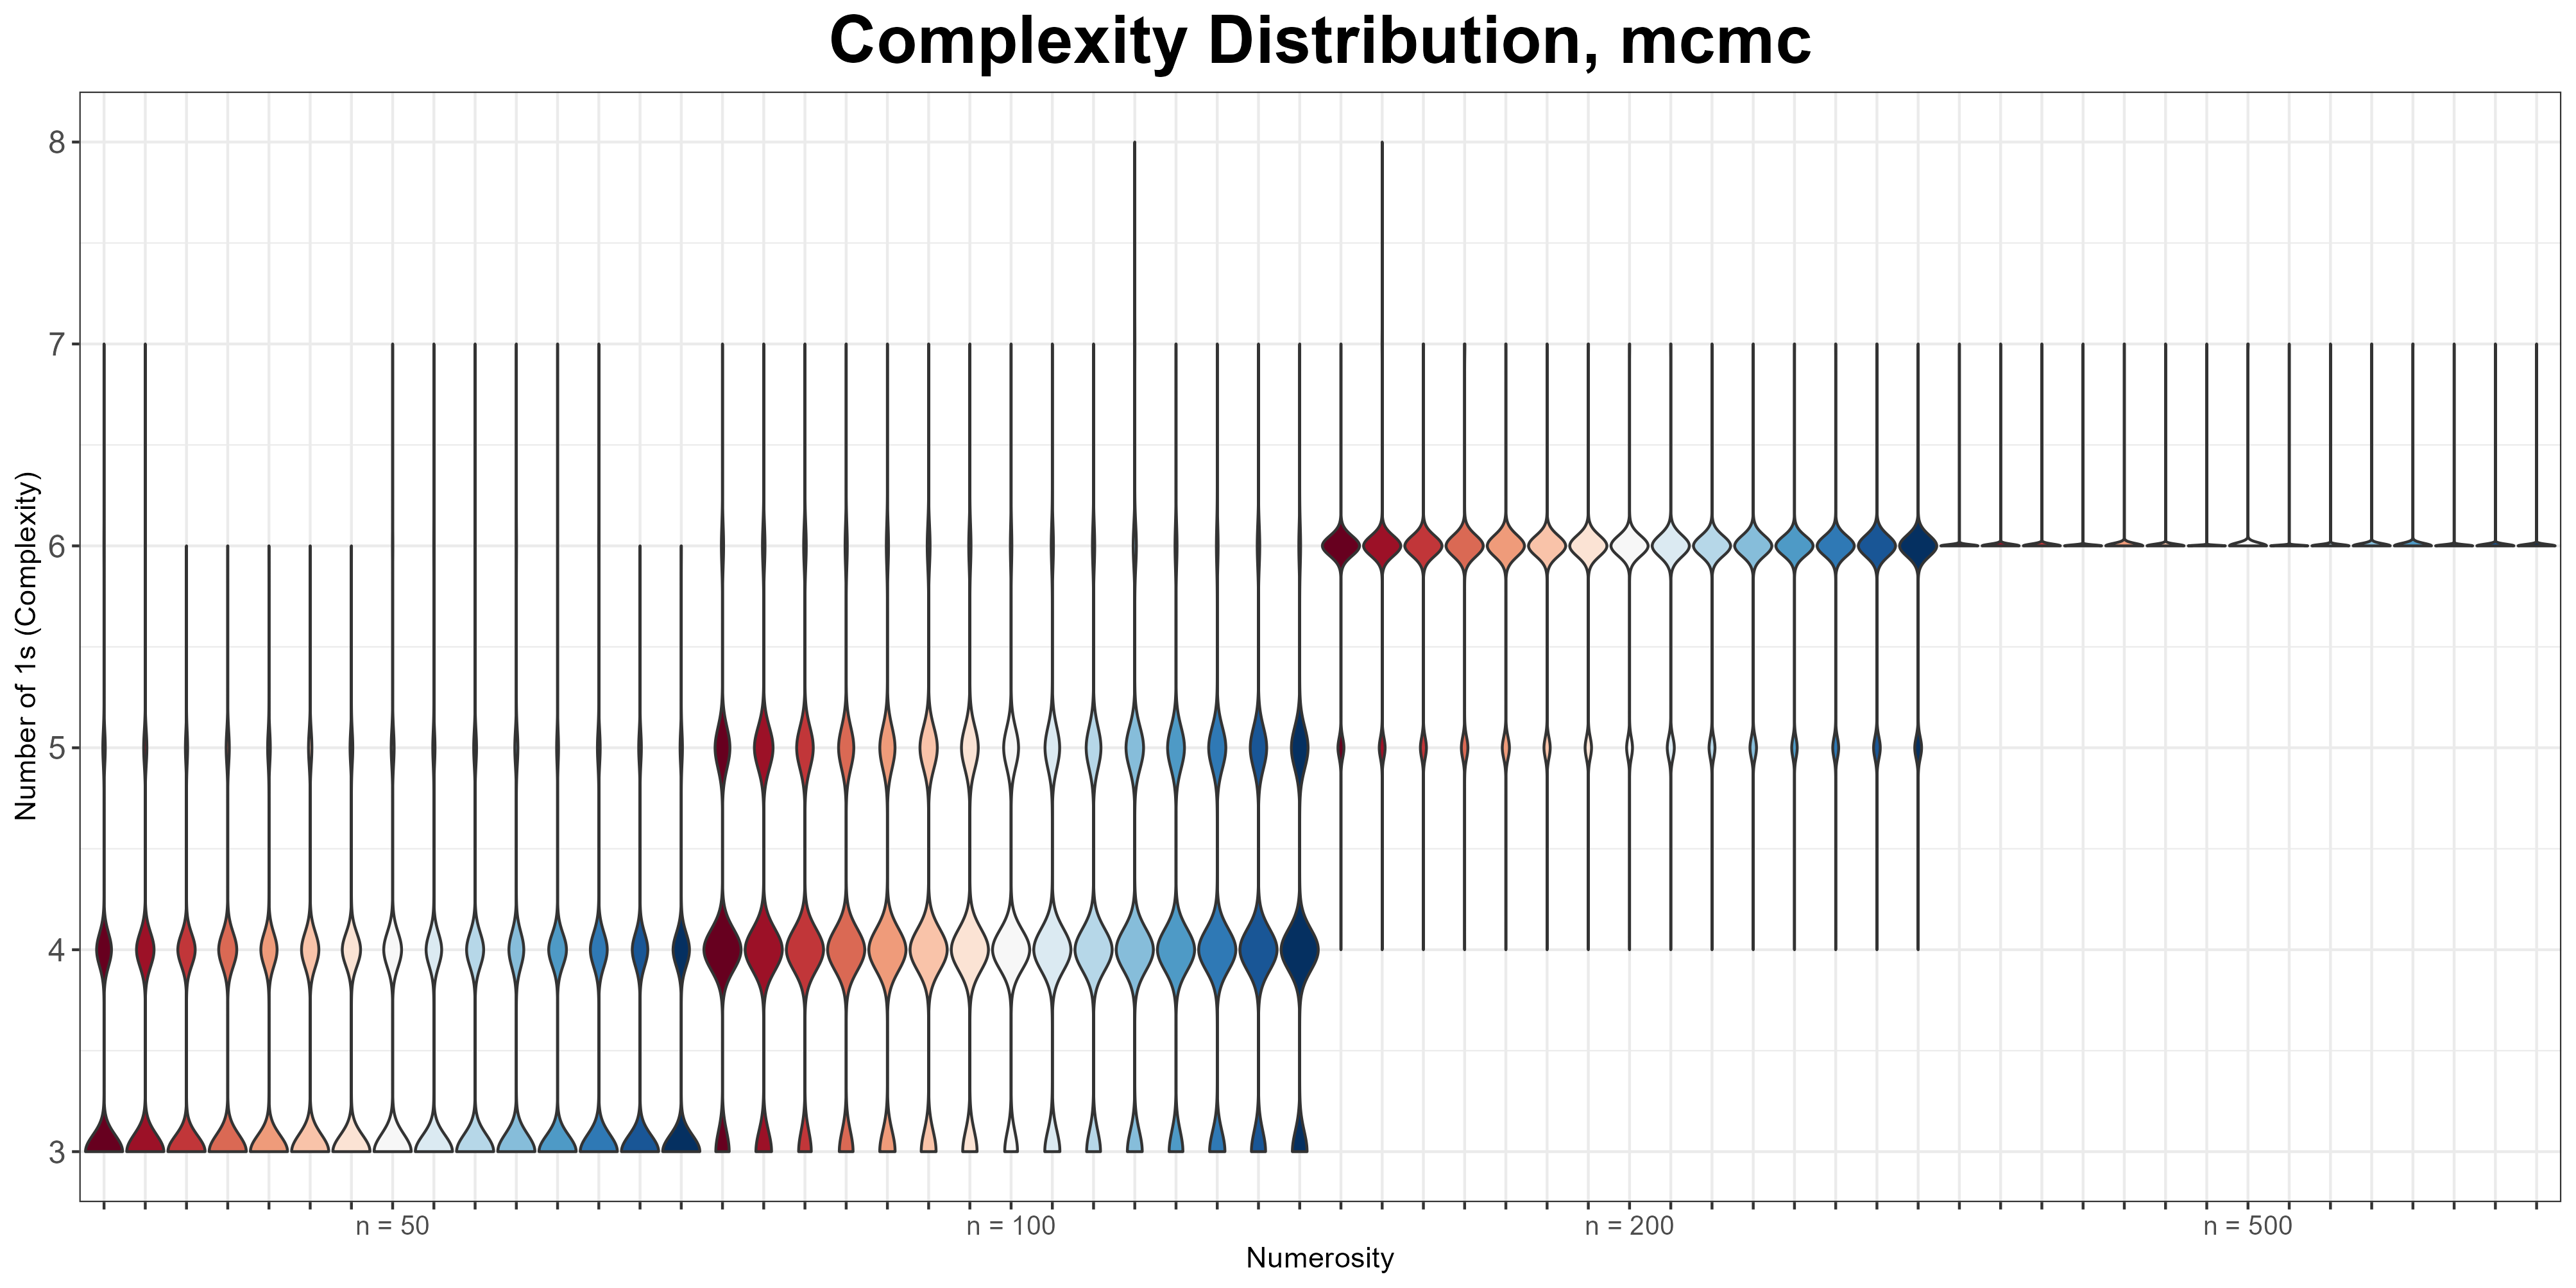
\includegraphics[height=4.1cm]{Figures/Diagnostic/Boxplot_compl_plain.png}
				%\caption{Plain metropolis}
				\label{fig:compl-plain}
			\end{subfigure}
			\hspace{0.35cm}  % horizontal space between figures
			% Second figure
			\begin{subfigure}[b]{0.45\textwidth}   
				\centering
				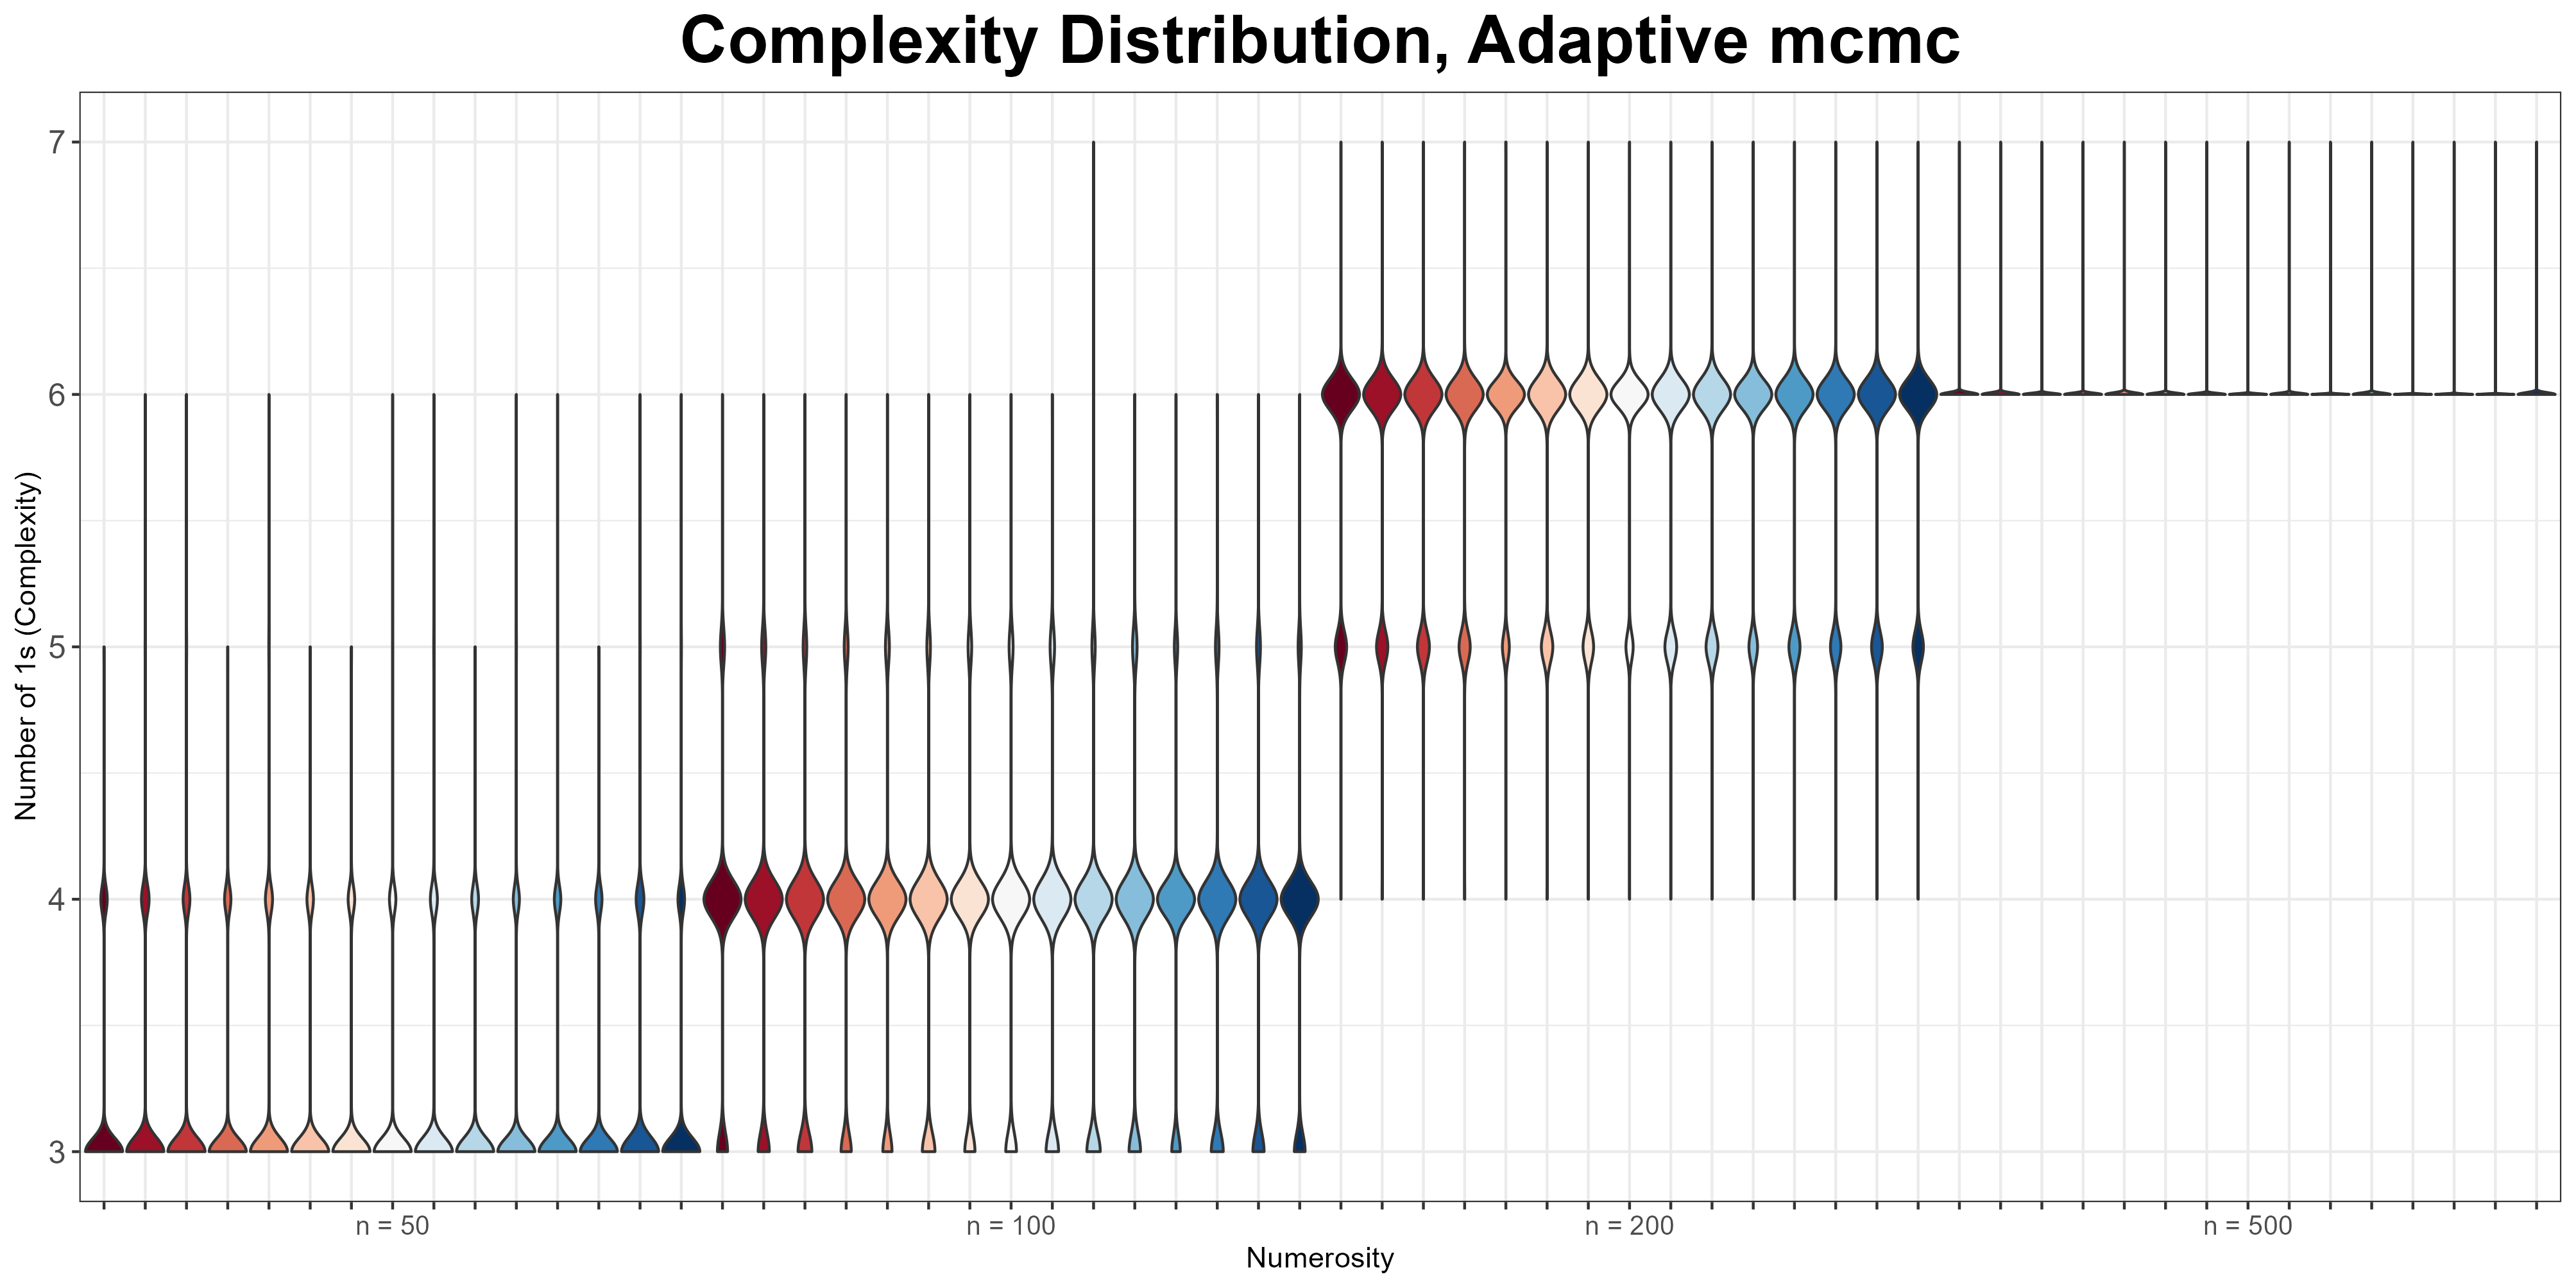
\includegraphics[height=4.1cm]{Figures/Diagnostic/Boxplot_compl_Adaptive.png}
				%\caption{Adaptive metropolis}
				\label{fig:compl-adaptive}
			\end{subfigure}
			
			\vspace{0.4cm}   %  vertical space between rows 
			
			% Third figure
			\begin{subfigure}[b]{0.45\textwidth}   
				\centering
				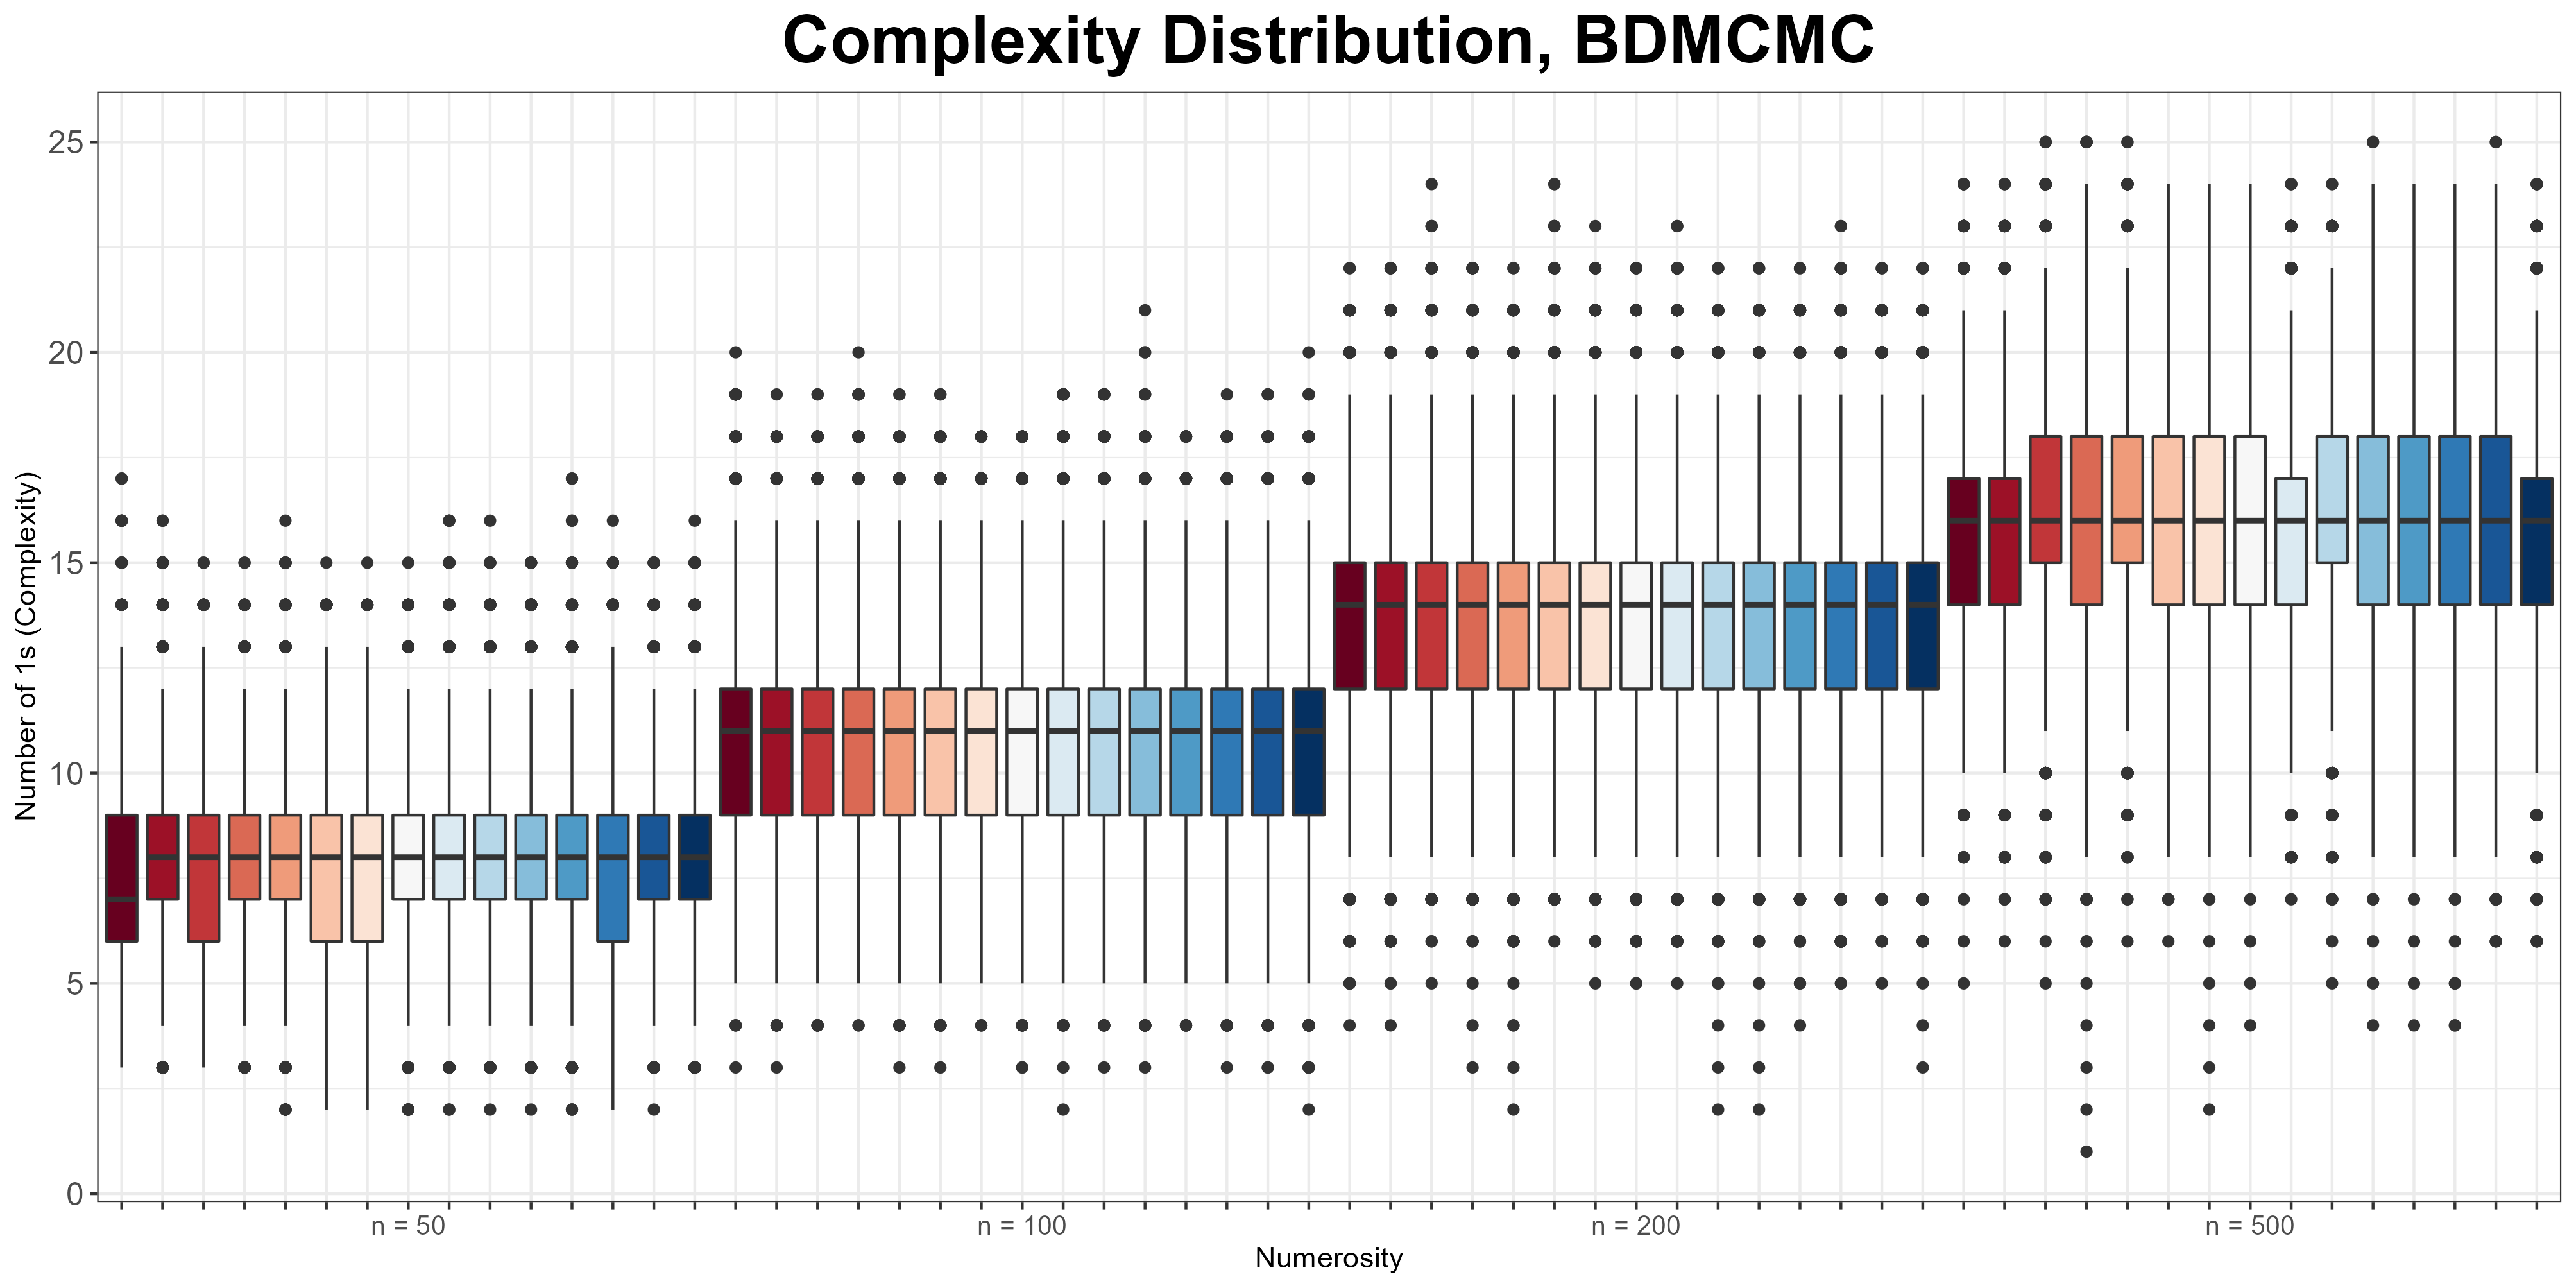
\includegraphics[height=4.1cm]{Figures/Diagnostic/Boxplot_compl_BD.png}
				%\caption{Birth-Death mcmc}
				\label{fig:compl-bd}
			\end{subfigure}
		\end{minipage}
	}
	\caption{Complexity distribution across algorithms}
	\label{fig:complexity}
\end{figure}

As depicted in \textit{Figure} \ref{fig:complexity}, the complexity distribution remains relatively stable across iterations within the same sample size, although variations are evident between different chains. Notably, as the sample size increases, the algorithms tend to explore larger graph configurations on average. This can be attributed to the algorithms' ability to leverage the additional data, which enhances their capacity to identify and sample from more complex structures in the graph space.

\subsection{Gelman-Rubin Diagnostic}

This approach assumes that $m$ chains are run in parallel, each starting from a different initial position that is overdispersed relative to the target distribution. As a result, the $m$ chains provide $m$ separate potential inferences. To evaluate whether these inferences are sufficiently similar to suggest approximate convergence, Gelman and Rubin proposed comparing them to the combined inference obtained by pooling together the $mn$ samples from all chains (\citet{brooks1998general}).
Specifically, the Potential Scale Reduction Factor (PSRF), often referred to as the Gelman-Rubin diagnostic, evaluates the convergence of multiple MCMC chains by comparing within-chain and between-chain variances. In the context of DAGs, this statistic is adapted to account for the binary nature of the data. If chains have converged, the within-chain variance should be approximately equal to the between-chain variance. The PSRF is computed as:

$$
\hat{R} = \sqrt{\frac{\hat{V}}{W}}
$$

where $W$ is the within-chain variance, and $\hat{V}$ s a weighted combination of within-chain and between-chain variances. This means that if the statistic is closed to one there is small variation across replicates. 

The Gelman-Rubin statistic is computed using 15 replicates for each numerosity, with the procedure repeated for all three algorithms. As shown in \textit{Figure} \ref{fig:gelman-rubic}, the variation in the statistic is consistently close to one for all edges, indicating convergence across chains, except for a few edges, which exhibit notable variation. This deviation may suggest that these particular edges are more sensitive to the sampling process or that they represent more complex relationships within the graph. The lack of convergence in these edges implies that the MCMC chains may not have sufficiently explored the configurations associated with those nodes, potentially leading to incomplete sampling of the underlying graph structure. 

Looking at this statistic, it appears that the BDMCMC presents more stable chains compared to the other two algorithms. This is because a smaller number of edges exhibit significant variance across replicates, indicating that the BDMCMC consistently explores similar graph structures. This behavior could be attributed to its ability to efficiently navigate the model space, reducing fluctuations by favoring more probable configurations. 

\begin{figure}[!ht]
	\centering
	\resizebox{\textwidth}{6.5cm}{  
		\begin{minipage}{\textwidth}
			\centering
			
			% First figure
			\begin{subfigure}[b]{0.45\textwidth}   
				\centering
				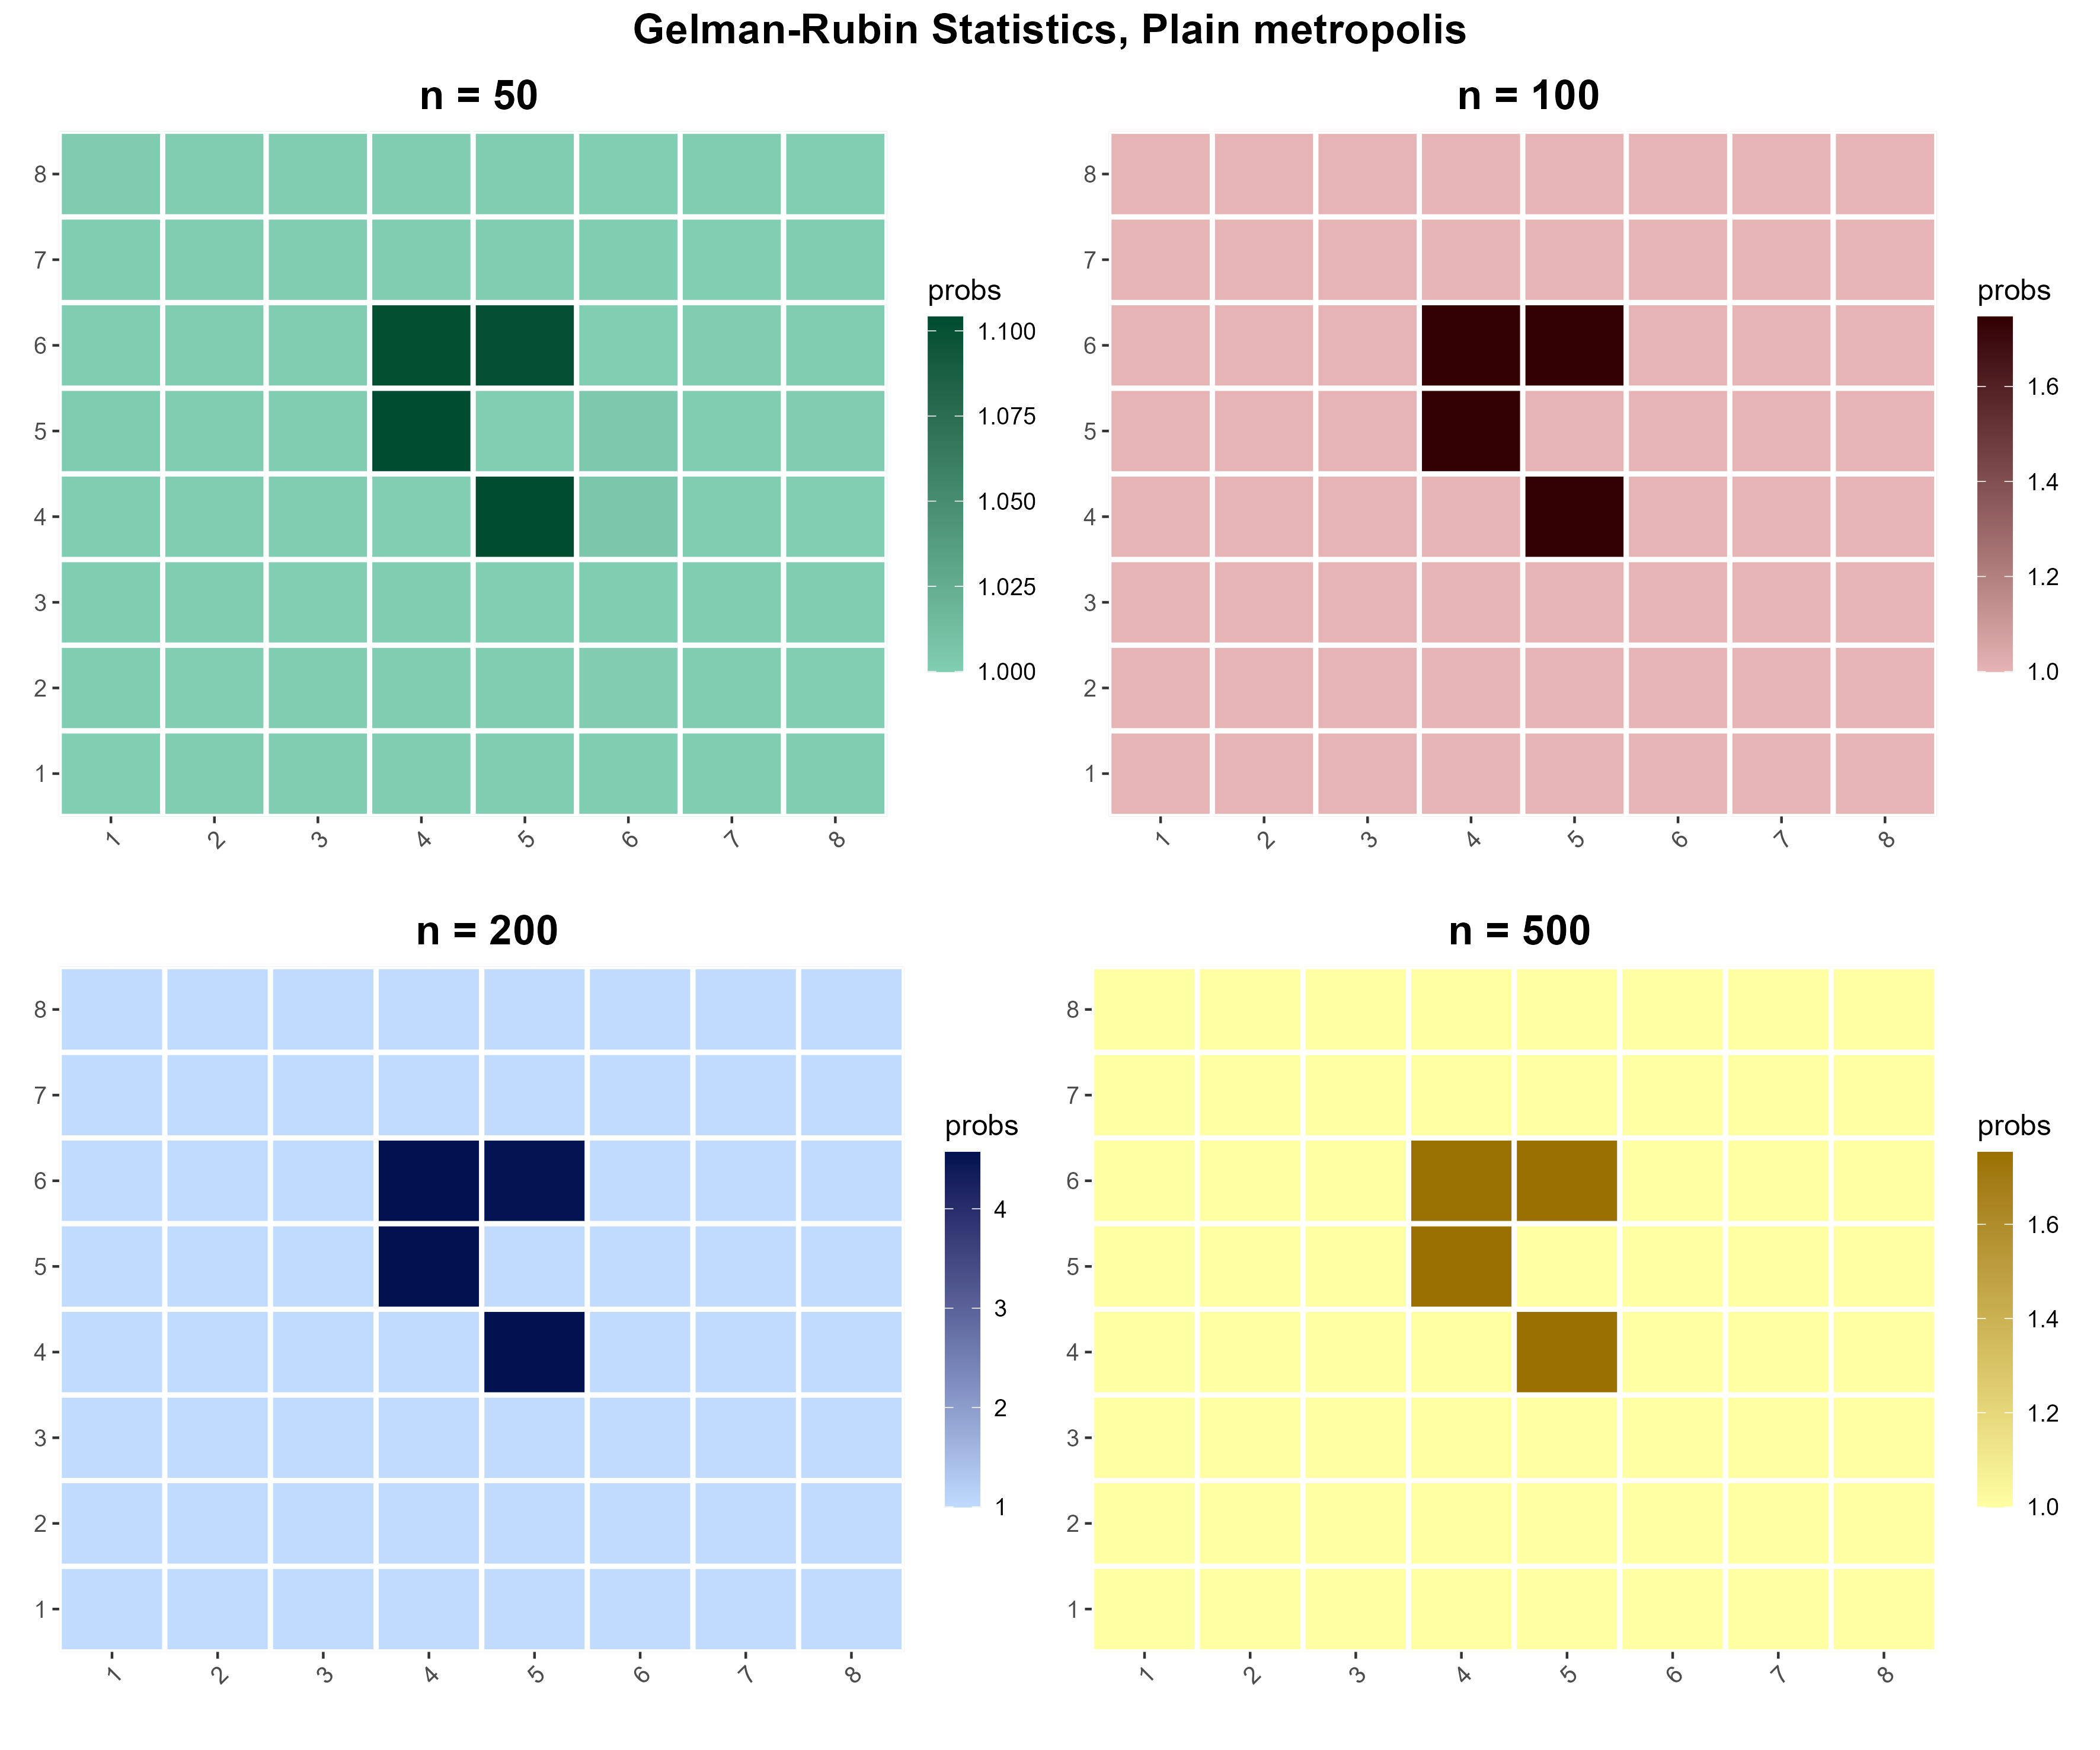
\includegraphics[height=4.1cm]{Figures/Diagnostic/gelmanRubic_plain.png}
				%\caption{Plain mcmc}
				\label{fig:gelmanr-plain}
			\end{subfigure}
			\hspace{0.35cm}  % horizontal space between figures
			% Second figure
			\begin{subfigure}[b]{0.45\textwidth}   
				\centering
				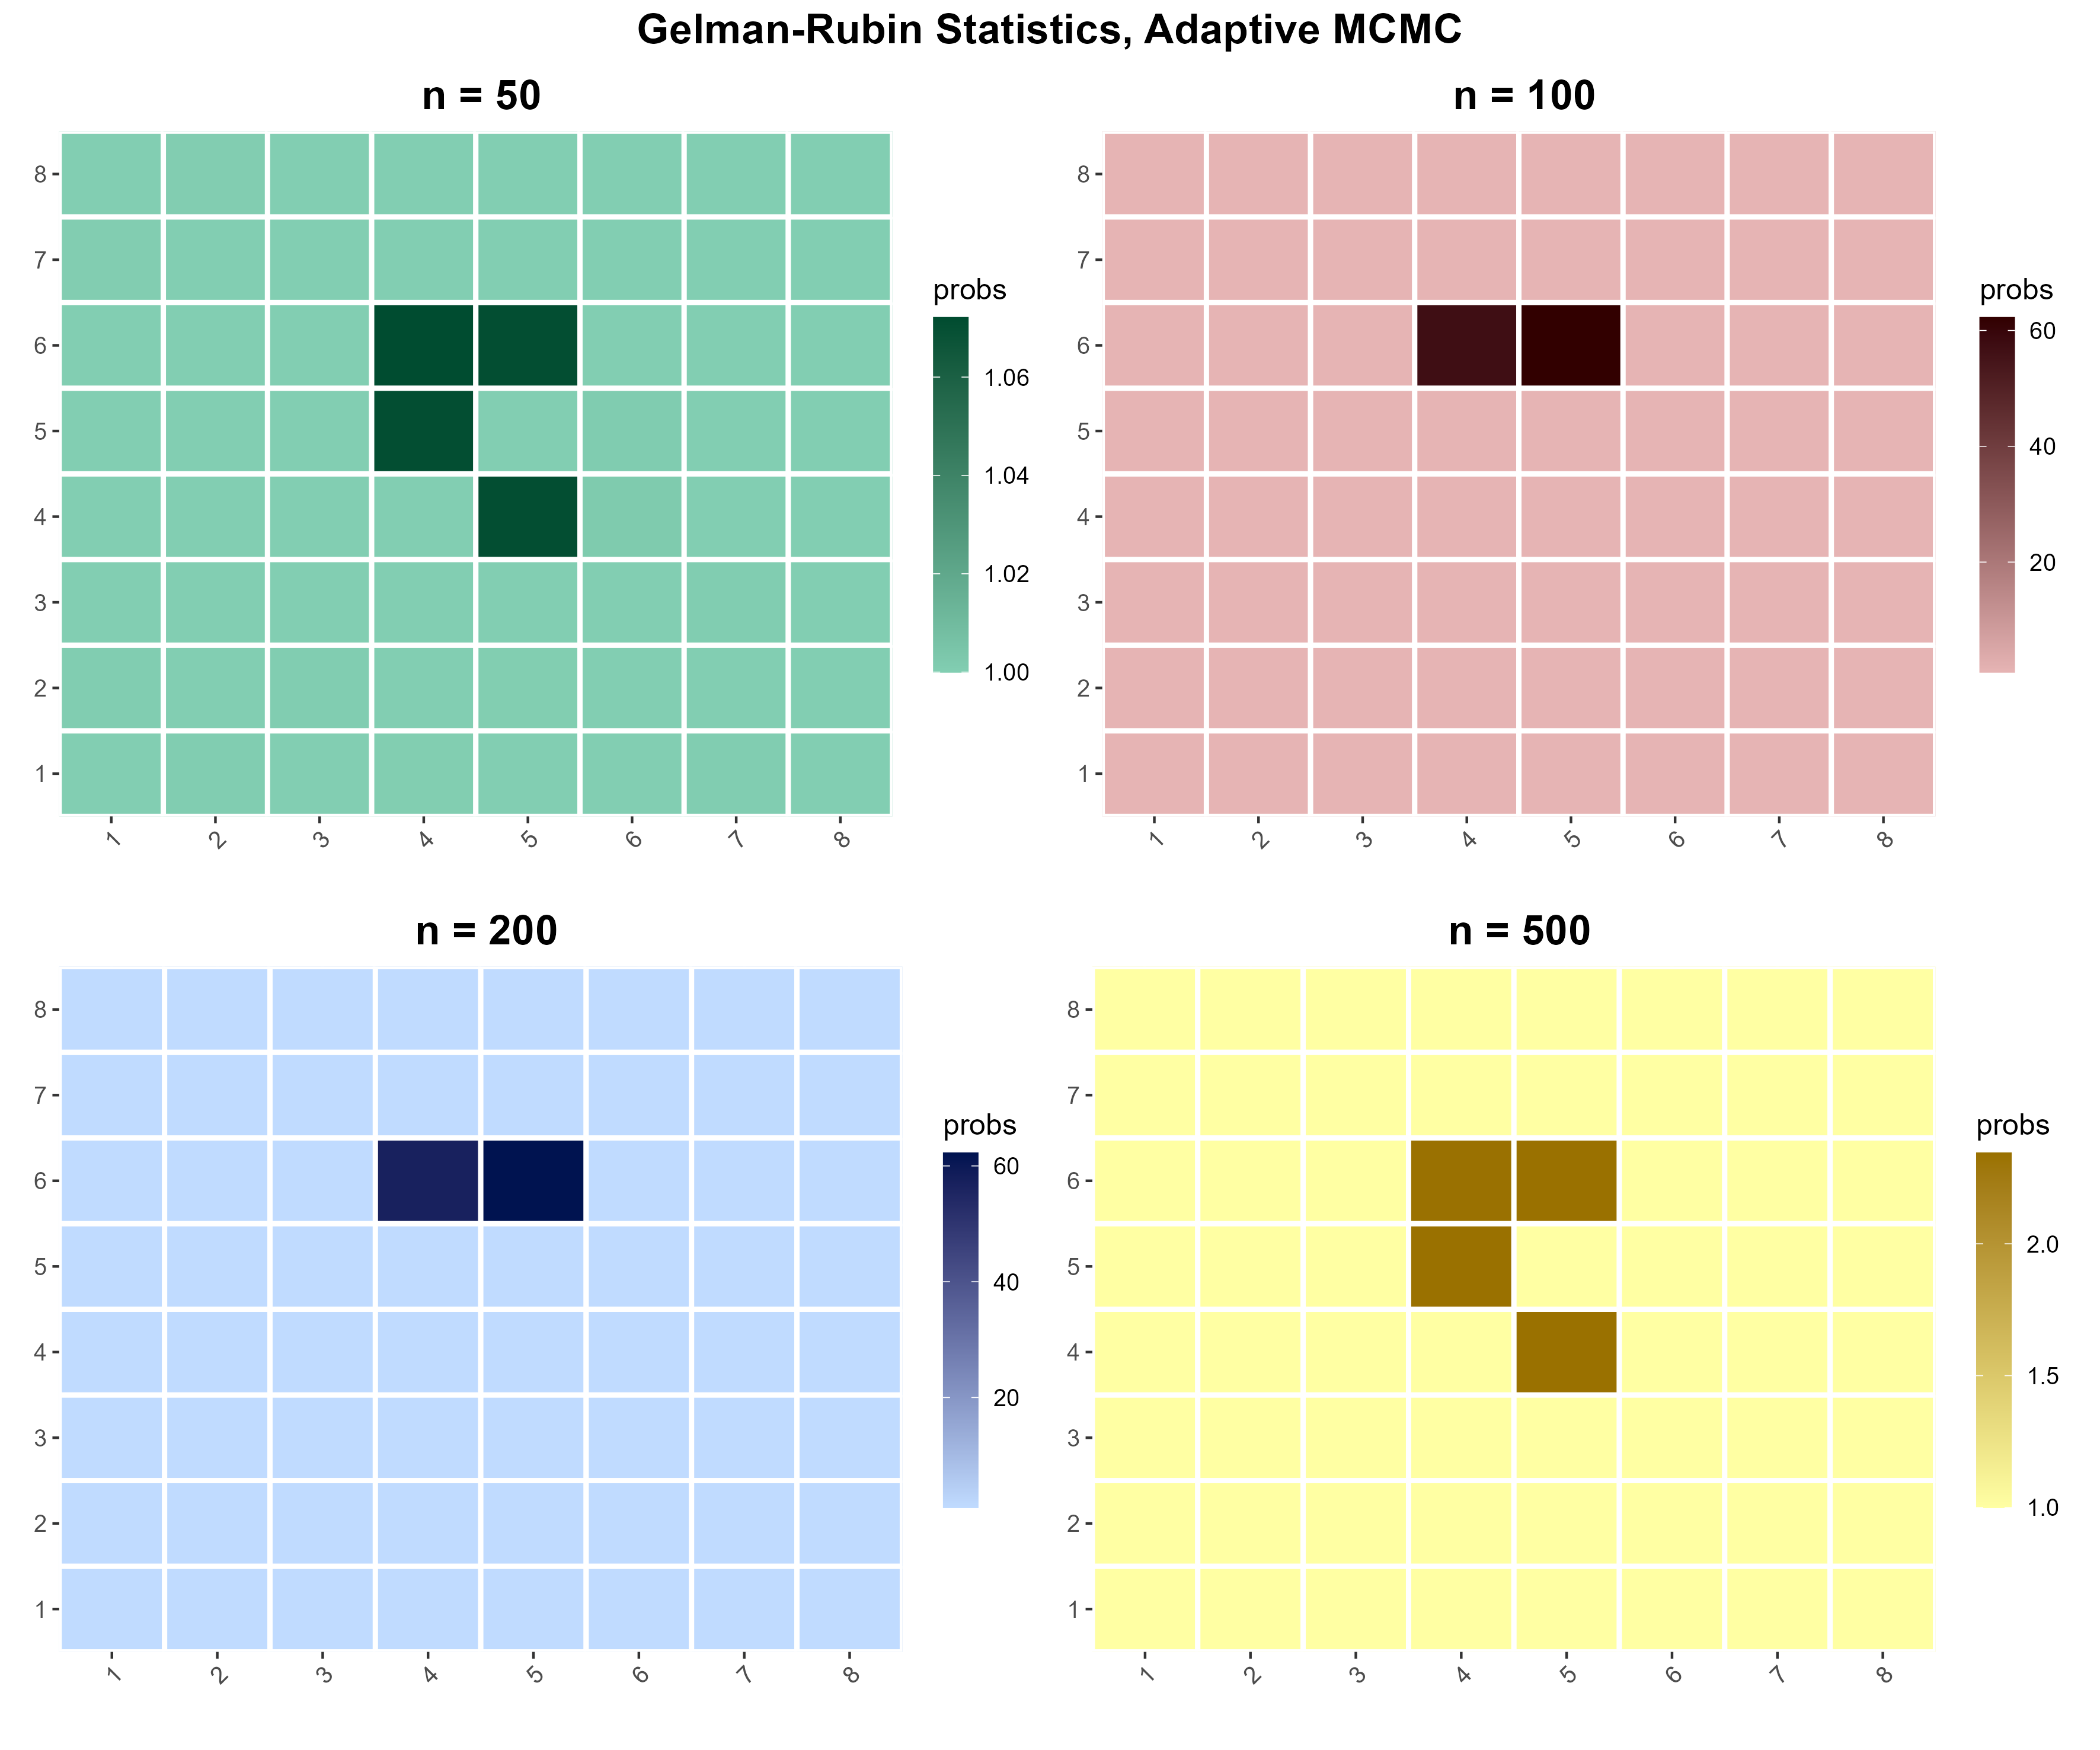
\includegraphics[height=4.1cm]{Figures/Diagnostic/gelmanRubic_Adaptive.png}
				%\caption{Adaptive mcmc}
				\label{fig:gelmanr-adaptive}
			\end{subfigure}
			
			\vspace{0.4cm}   %  vertical space between rows 
			
			% Third figure
			\begin{subfigure}[b]{0.45\textwidth}   
				\centering
				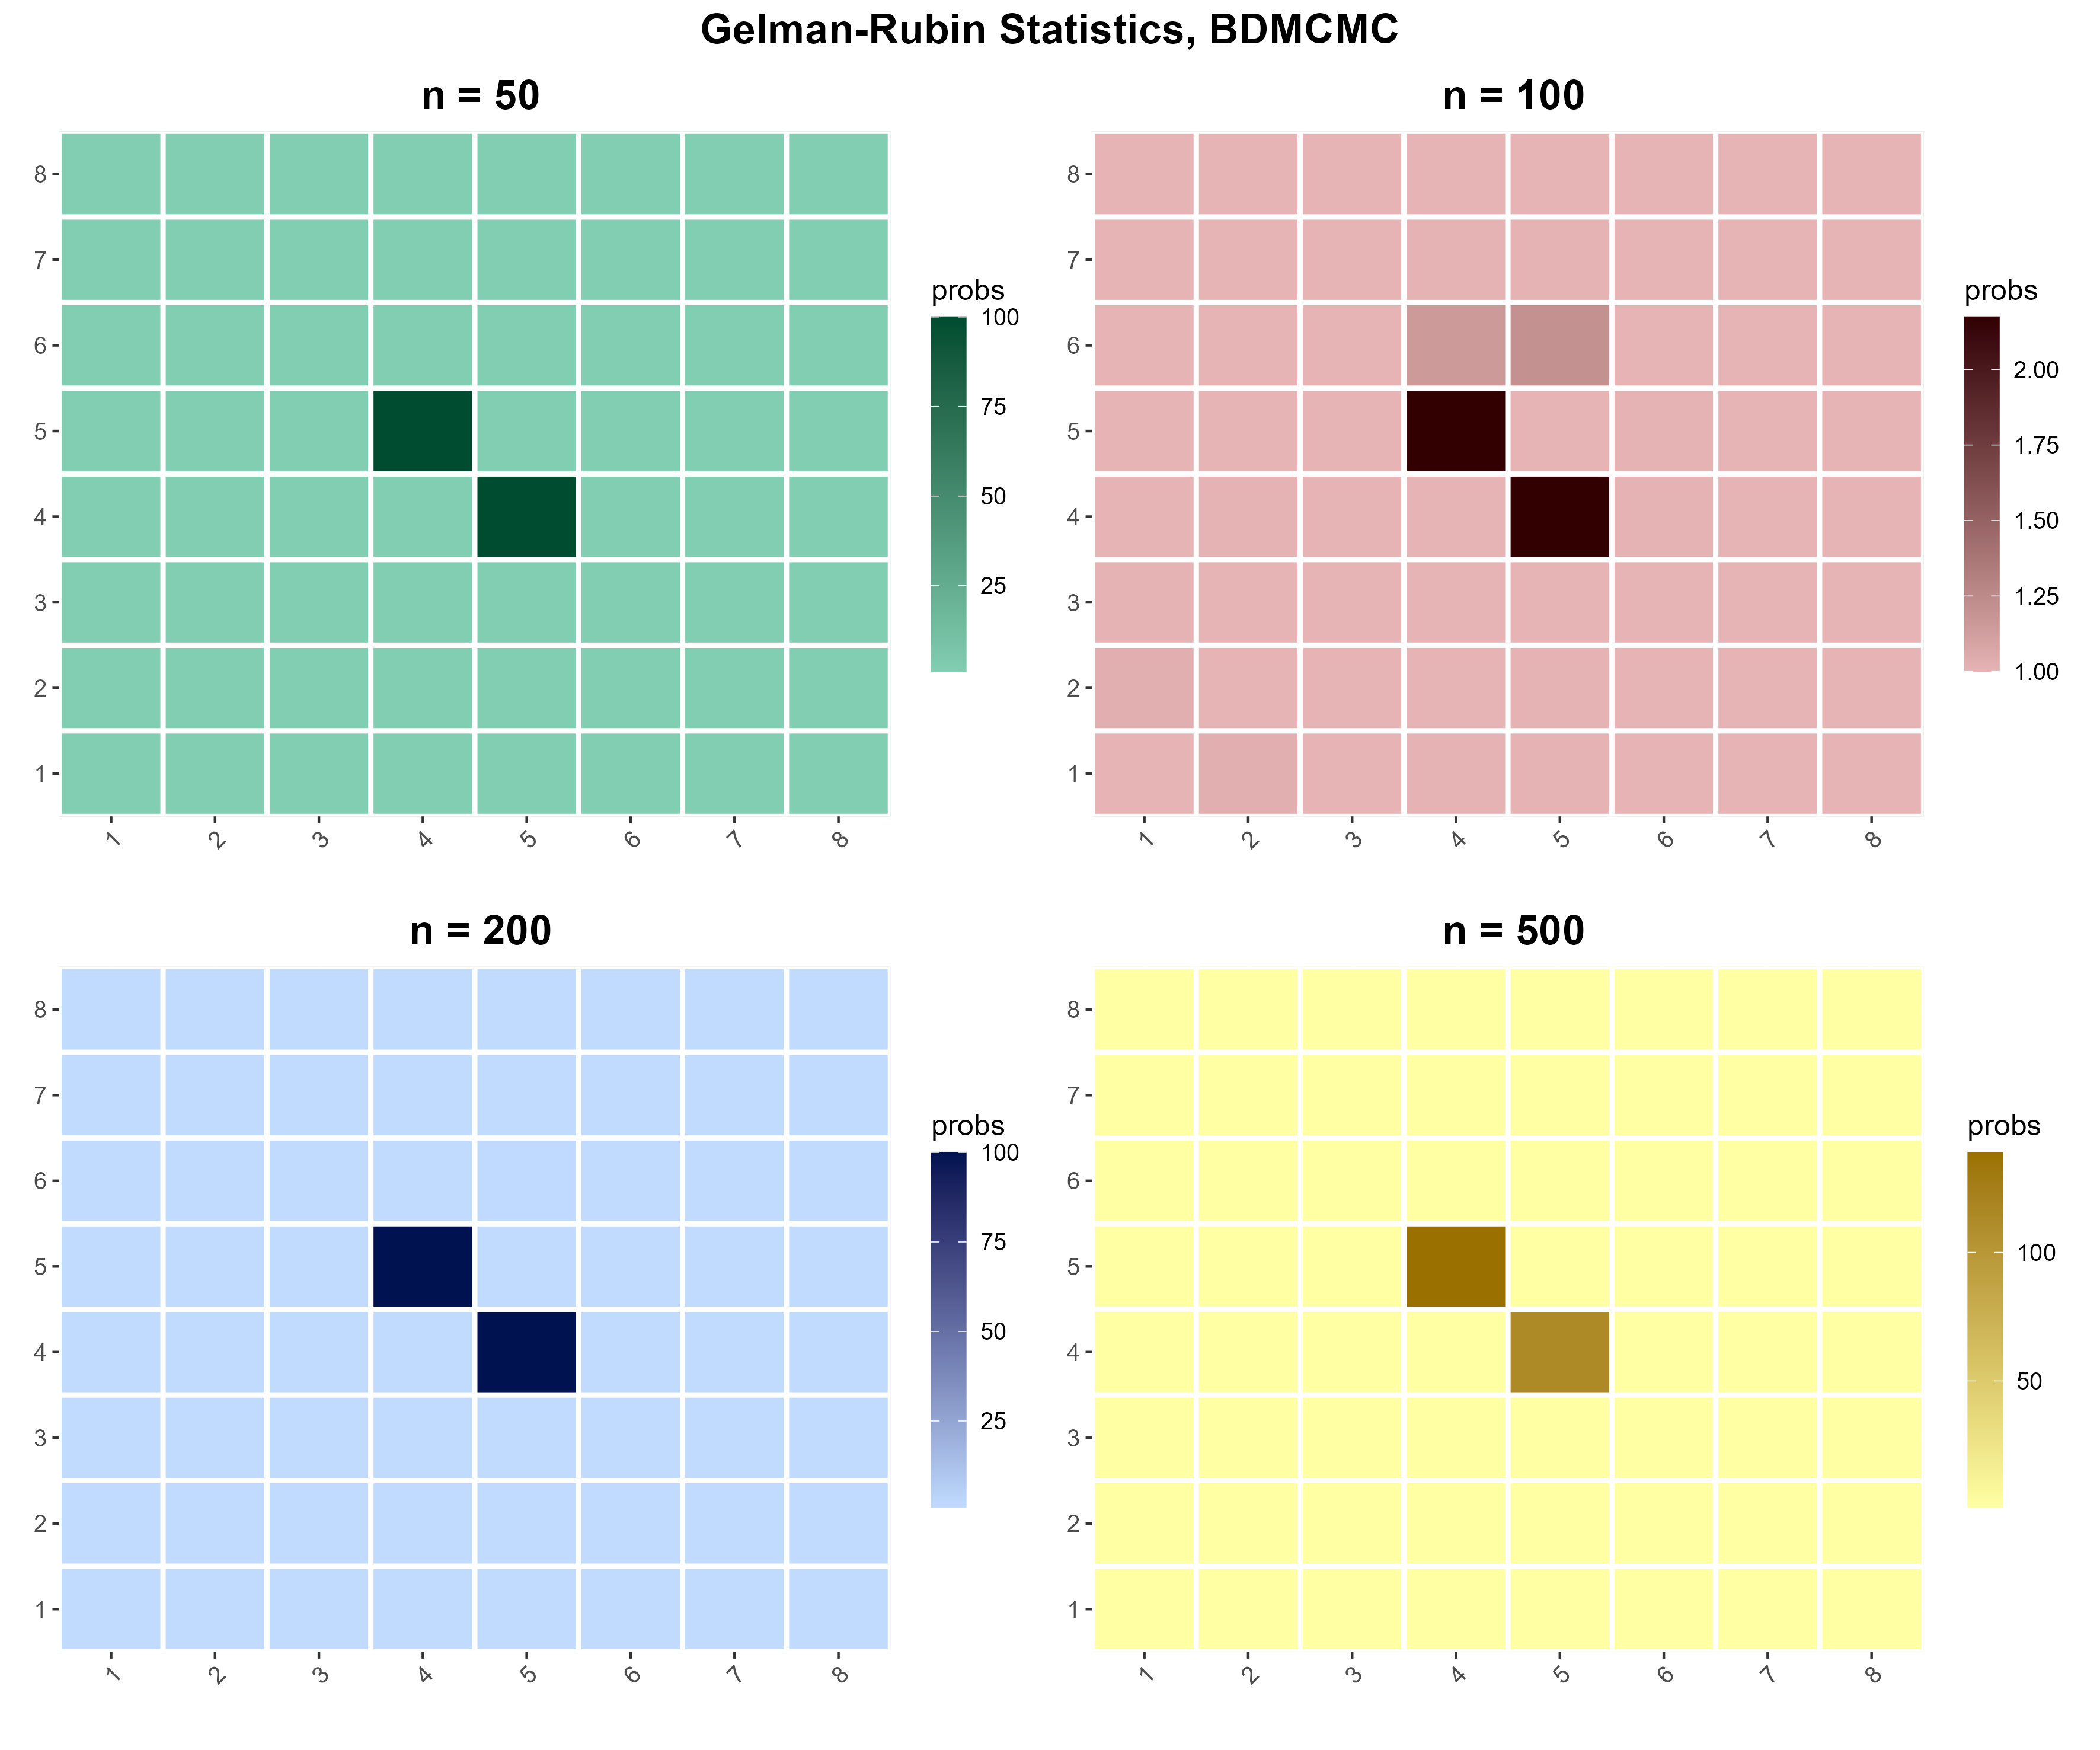
\includegraphics[height=4.1cm]{Figures/Diagnostic/gelmanRubic_BDMCMC.png}
				%\caption{Birth-Death mcmc}
				\label{fig:gelmanr-bd}
			\end{subfigure}
		\end{minipage}
	}
	\caption{Gelman-rubic statistic across algorithms.}
	\label{fig:gelman-rubic}
\end{figure}

\subsection{Hellinger Distance}

The Hellinger distance is a measure of similarity between two probability distributions, used here to compare consecutive DAGs. In each iteration of the MCMC process, the adjacency matrix of the DAG is treated as a vector, and the Hellinger distance quantifies how the structure of the DAG evolves. This distance is particularly useful for monitoring whether the chain is transitioning smoothly between models, indicating stable exploration. For
two probability distributions $p$ and $q$ the Hellinger distance $H(p,q)$ is defined as (\citet{boone2014hellinger}):

$$
H(p,q) = \sqrt{0.5 \sum_{i} (\sqrt{p_i} - \sqrt{q_i})^2}
$$

where $p_i$ and $q_i$ represent the probability mass functions of two consecutive DAG structures.

\begin{figure}[!ht]
	\centering
	\resizebox{\textwidth}{6.5cm}{  
		\begin{minipage}{\textwidth}
			\centering
			
			% First figure
			\begin{subfigure}[b]{0.45\textwidth}   
				\centering
				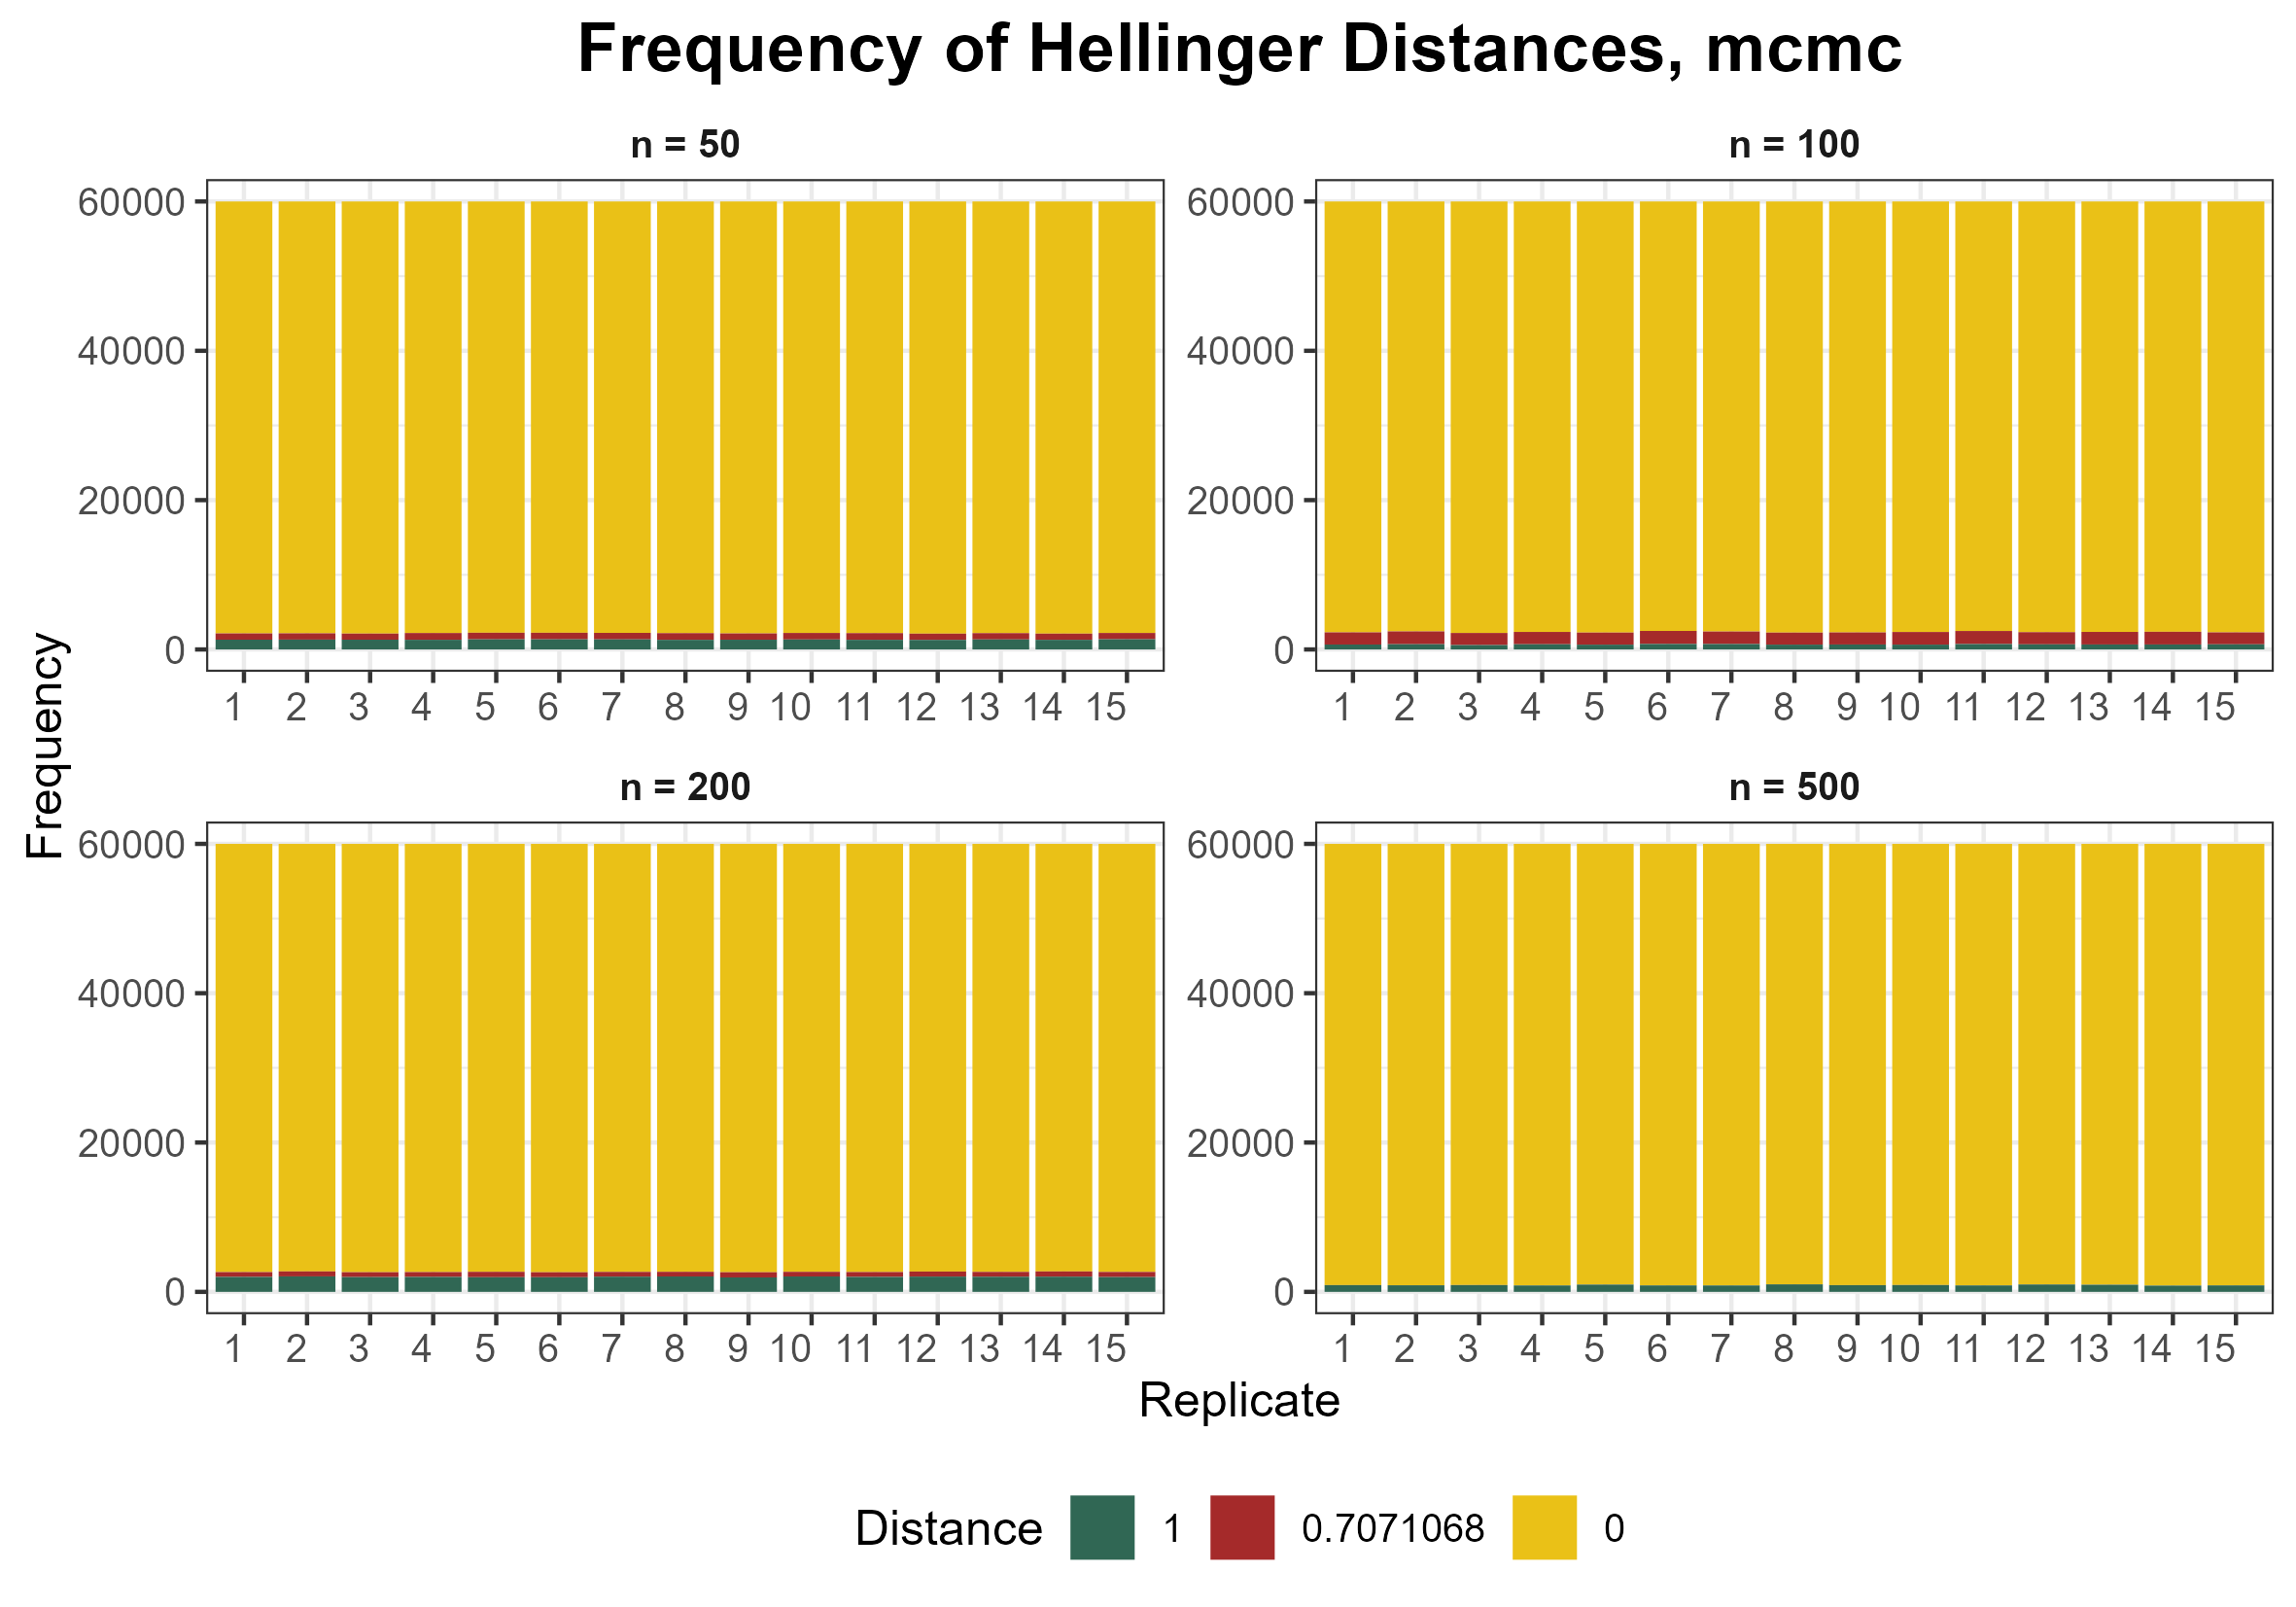
\includegraphics[height=4.1cm]{Figures/Diagnostic/Hellinger_distance_plain.png}
				%\caption{Plain metropolis}
				\label{fig:hellinger-plain}
			\end{subfigure}
			\hspace{0.35cm}  % horizontal space between figures
			% Second figure
			\begin{subfigure}[b]{0.45\textwidth}   
				\centering
				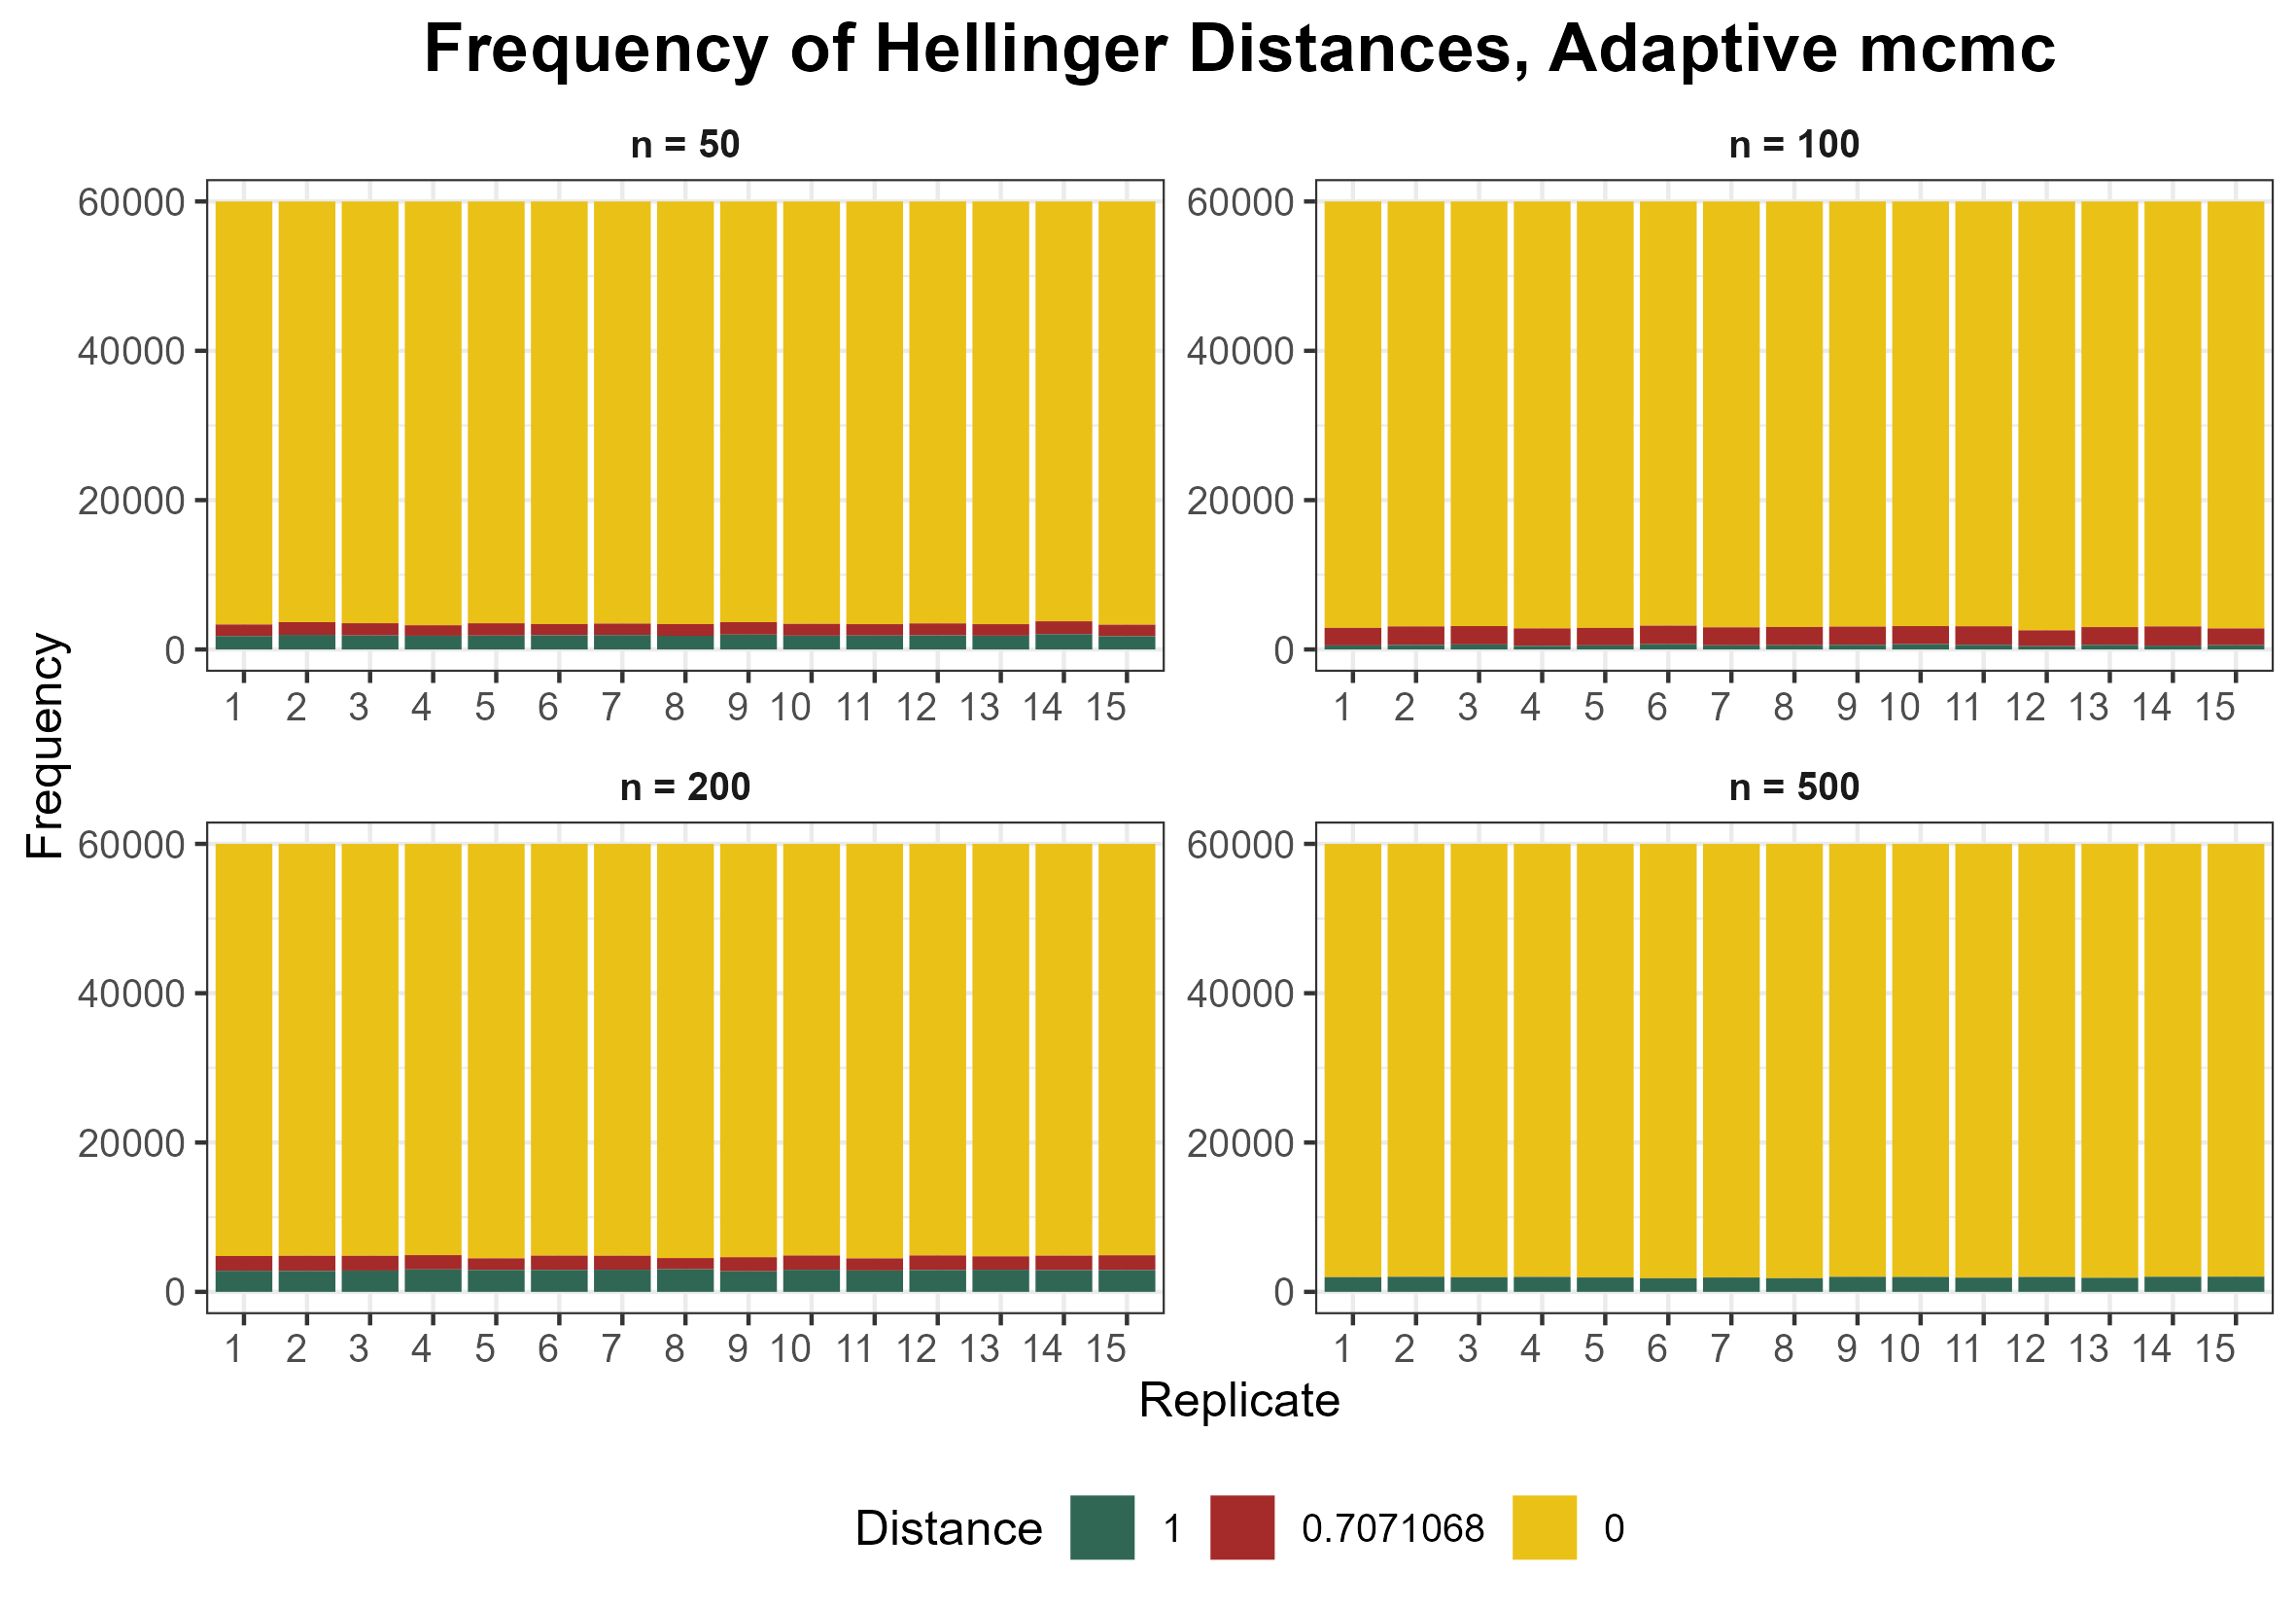
\includegraphics[height=4.1cm]{Figures/Diagnostic/Hellinger_distance_Adaptive.png}
				%\caption{Adaptive metropolis}
				\label{fig:hellinger-adaptive}
			\end{subfigure}
			
			\vspace{0.4cm}   %  vertical space between rows 
			
			% Third figure
			\begin{subfigure}[b]{0.45\textwidth}   
				\centering
				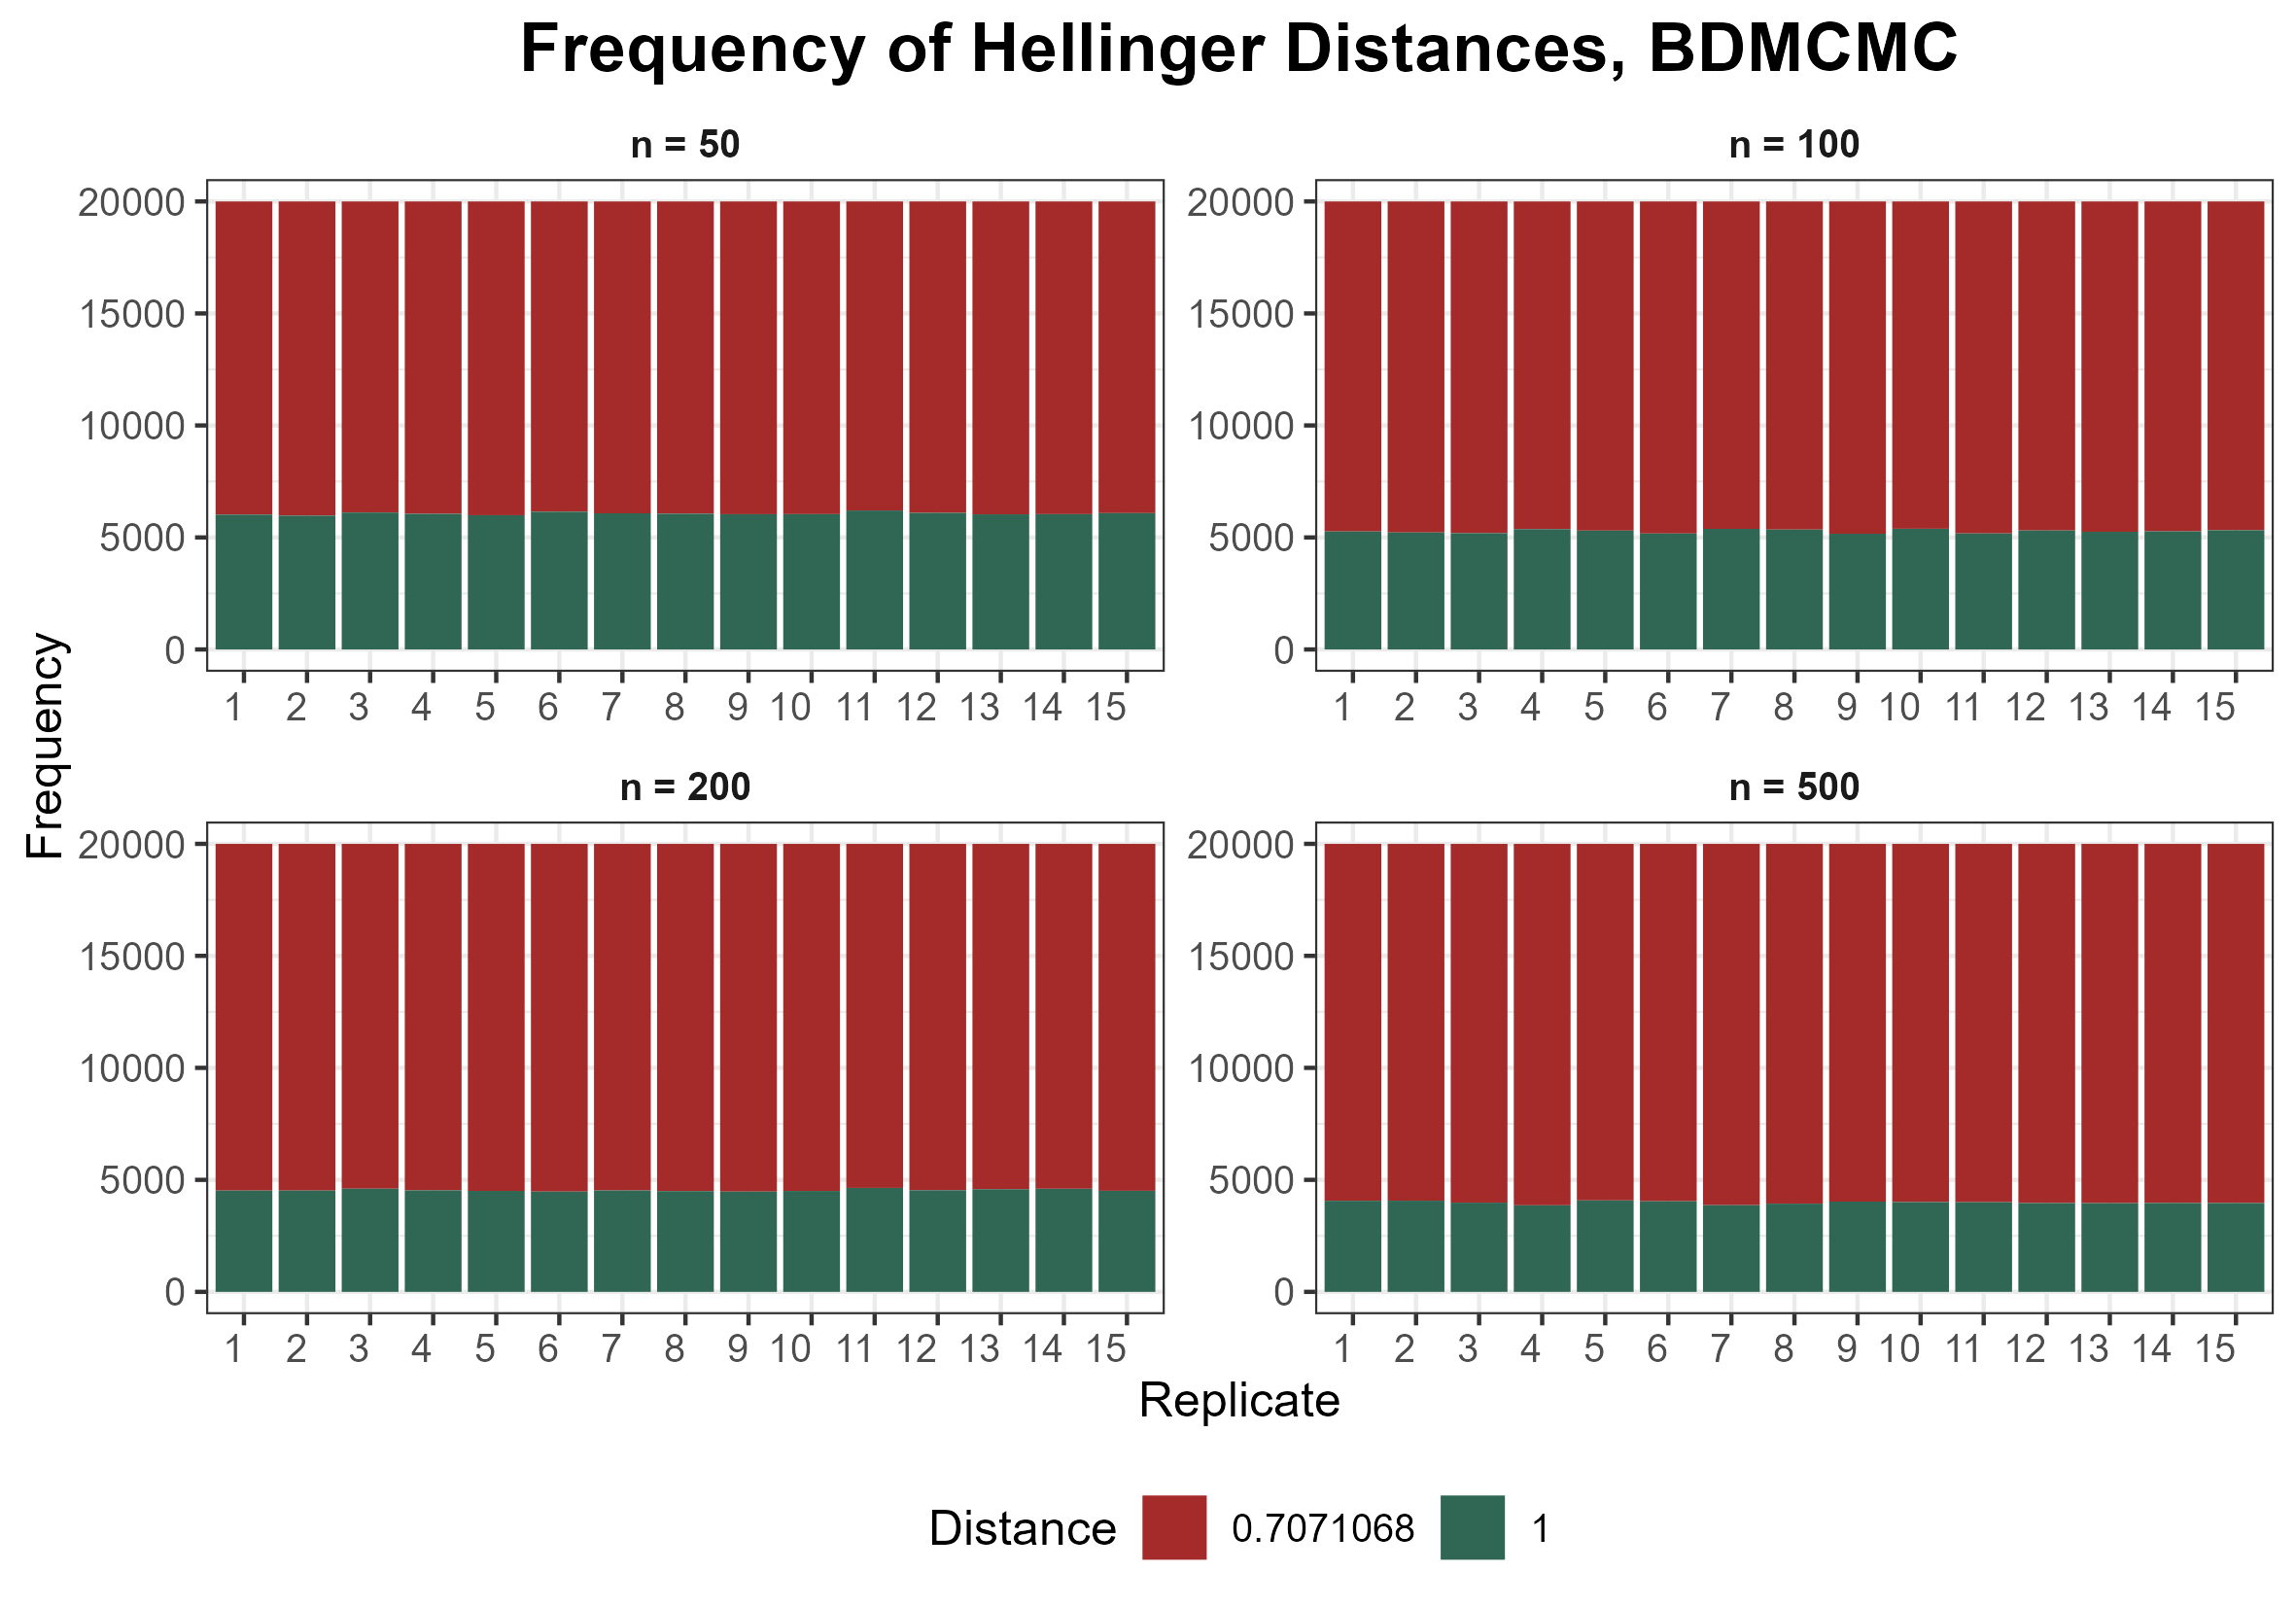
\includegraphics[height=4.1cm]{Figures/Diagnostic/Hellinger_distance_BD.png}
				%\caption{Birth-Death mcmc}
				\label{fig:hellinger-bd}
			\end{subfigure}
		\end{minipage}
	}
	\caption{Frequency of hellinger distances}
	\label{fig:hellinger}
\end{figure}

Its range is from 0 to 1, where a distance of 0 indicates that the distributions are identical, while a distance of 1 signifies complete dissimilarity. As illustrated in \textit{Figure}  \ref{fig:hellinger}, the Hellinger distance takes on three distinct values: the two extremes (0 and 1) and 0.7. In the context of these algorithms, a distance of 0 signifies that the graph configuration has not changed between iterations. This scenario is not allowed by construction in the BDMCMC, which forces acceptance of every proposed move, whereas the other two schemes permit rejections, resulting in the chains occasionally remaining in the same state. By contrast, a value of 1 appears when the two DAGs are entirely different in terms of their adjacency matrices, this occurring when a reverse operation takes place.  Finally, the intermediate value of 0.7 arises when a local move, such as adding or deleting a single edge, is performed. This indicates that while the graph structure is altered, the change is relatively minor, and the adjacency matrices still share a substantial overlap.

\begin{table}[htp]
	\centering
	
	\begin{tabular}{
			p{2.5cm}
			S[table-format=1.4, round-mode=places, round-precision=4]
			S[table-format=1.4, round-mode=places, round-precision=4]
			S[table-format=1.4, round-mode=places, round-precision=4]
			S[table-format=1.4, round-mode=places, round-precision=4]
			@{}
		}
		\toprule
		& {n = 50} & {n = 100} & {n = 200} & {n = 500} \\
		\midrule
		\multicolumn{4}{@{}l}{\textit{Plain metropolis}} \\
		Rejection & 0.9637005061 & 0.9610460174 & 0.9554114791 & 0.9848186359 \\
		Add / Delete & 0.0143246832 & 0.0276871281 & 0.0110746290 & 0.0001044462 \\
		Reverse & 0.0219748107 & 0.0112668544 & 0.0335138919 & 0.0150769179 \\
		\midrule
		\multicolumn{4}{@{}l}{\textit{Adaptive metropolis}} \\
		Rejection & 0.9422945938 & 0.9503113941 & 0.9205986766 & 0.9672616766 \\
		Add / Delete & 0.0263348834 & 0.0399684439 & 0.0309294044 & 0.0002444485 \\
		Reverse & 0.0313705228 & 0.0097201620 & 0.0484719190 & 0.0324938749 \\
		\midrule
		\multicolumn{4}{@{}l}{\textit{BDMCMC}} \\
		Add / Delete & 0.6966948 & 0.7361101 & 0.7731987 & 0.8005834 \\
		Reverse & 0.3033052 & 0.2638899 & 0.2268013 & 0.1994166 \\
		\bottomrule
	\end{tabular}
	
	\caption{Mean Hellinger distance frequencies across replicates for the three algorithms.}
	\label{table:hellinger-table}
	
\end{table}

As shown in \ref{table:hellinger-table}, both the plain MCMC and adaptive chains demonstrate an increasing number of rejections with higher numerosity, resulting in instances where the Hellinger distance equals zero. This outcome suggests a detrimental effect on the performance of both addition and reverse operators, indicating that the chains frequently encounter rejections. Such behavior is likely due to the algorithm's difficulty in identifying suitable moves within the complex and vast model space.

In the case of the plain Metropolis algorithm, more addition operations are performed compared to reverse operations. Conversely, the adaptive chain exhibits the opposite behavior.
In the context of the BDMCMC, as the sample size increases, the gap between the addition and reverse operations widens, consistently favoring the addition operations. This trend is likely because the additional data provides more information for the algorithm to effectively identify beneficial edges to add, enhancing the overall complexity of the graph structures.

\subsection{Kolmogorov-Smirnov (K-S) Statistic}

The Kolmogorov-Smirnov (K-S) statistic is a non-parametric test used to compare two empirical distributions, in this case, the distributions of model indicators obtained from two different Markov chains. The test is based on the maximum difference between an empirical and a hypothetical cumulative distribution (\citet{massey1951kolmogorov}).
The purpose of applying the K-S statistic here is to determine if the two chains have converged to the same posterior distribution by evaluating the difference between their cumulative distribution functions. In the context of DAGs, each directed acyclic graph is represented as a binary matrix, which is then flattened into a vector. This binary vector can be thought of as a unique identifier for the model, as a result, it can be transformed into a decimal model indicator. By computing this statistic across different iterations, it is then possible to measure how closely the two chains align at various stages, providing insight into whether both chains are sampling from the same posterior distribution.

The K-S statistic $D_{n,m}$ between two cumulative distributions $F_n (x)$ and $G_m (x)$ is given by:

$$
D_{n,m} = \sup_x |F_n (x) - G_m (x)|
$$

where $n$ and $m$ are the number of samples in the two chains being compared.

The vector of model indicators, $M_i$, is treated as a number expressed in base $d$, and converted to its decimal equivalent, $P$, by setting the transformation:

$$
P(M_i) = 1 + \sum^k_{j=1} m_i (j) d^{j-1} \in \{1,2, ... , d^k\}
$$

In the case of DAGs, where each element in the adjacency matrix is either 0 or 1, the transformation $P(M_i)$ treats the flattened matrix as a binary number. Each entry of the flattened matrix, $m_i(j)$, represents a bit in this binary sequence. The sum $\sum^k_{j=1} m_i (j) d^{j-1}$ becomes a sum of powers of 2, since $d = 2$ for binary DAGs. 

For example, consider a $2 \times 2$ binary DAG with a flattened vector $M_i = [1, 0, 1, 1]$. The transformation to the decimal equivalent $P(M_i)$ would be:

$$
P(M_i) = 1 + (1 \cdot 2^0) + (0 \cdot 2^1) + (1 \cdot 2^2) + (1 \cdot 2^3) = 1 + 1 + 0 + 4 + 8 = 14 
$$

From $P(M_i)$ it is then possible to recover $M_i$ by iteratively solving the equation:

$$
1 + \sum^k_{j=1} m_i (j) d^{j-1} = P
$$

The inversion is done as follows (\citet{brooks2003nonparametric}):

\begin{enumerate}
	\item Initialization: Set $\lambda_k = P - 1$ and find the largest $h \in {0, \dots, d-1}$ such that $\lambda_k \geq h d^{k-1}$, and set $m_i(k) = h$. Now consider $j = k-1$.
	\item Set $\lambda_j = \lambda_{j+1} - m_i(j+1) d^j$, and find the largest $h \in {0, \dots, d-1}$ such that $\lambda_j \geq h d^{j-1}$, and set $m_i(j) = h$.
	\item If $j = 1$, set $j = j - 1$ and return to Step 2, otherwise stop.
\end{enumerate}

In addition, thinning the chain is a crucial passage as the K-S statistic assumes independent data. The idea is to select every k-th sample from the original chain, where k is determined based on the autocorrelation structure of the model indicators.
To compute $k$, the autocorrelation function (ACF) of the model indicators is estimated, and the decay rate, $\lambda$, is obtained by fitting an exponential decay model of the form:

$$
ACF(t) \sim e^{-\lambda t}
$$

The thinning parameter $k$ is then chosen so that the dependence between the selected samples is negligible. Specifically, $k$ is calculated as:

$$
k = \biggr[ \frac{log 0.01}{log \lambda} \biggr]
$$

In simpler terms the estimate $\lambda$ is used to quantify how quickly the chain "forgets" its past. This ensures that the dependence between two samples spaced k steps apart is reduced to around $1\%$ of their initial correlation. The choice of 0.01 corresponds to an error level at which the chain is sufficiently close to stationarity.



\begin{figure}[!ht]
	\centering
	\resizebox{\textwidth}{6.5cm}{  
		\begin{minipage}{\textwidth}
			\centering
			
			% First figure
			\begin{subfigure}[b]{0.45\textwidth}   
				\centering
				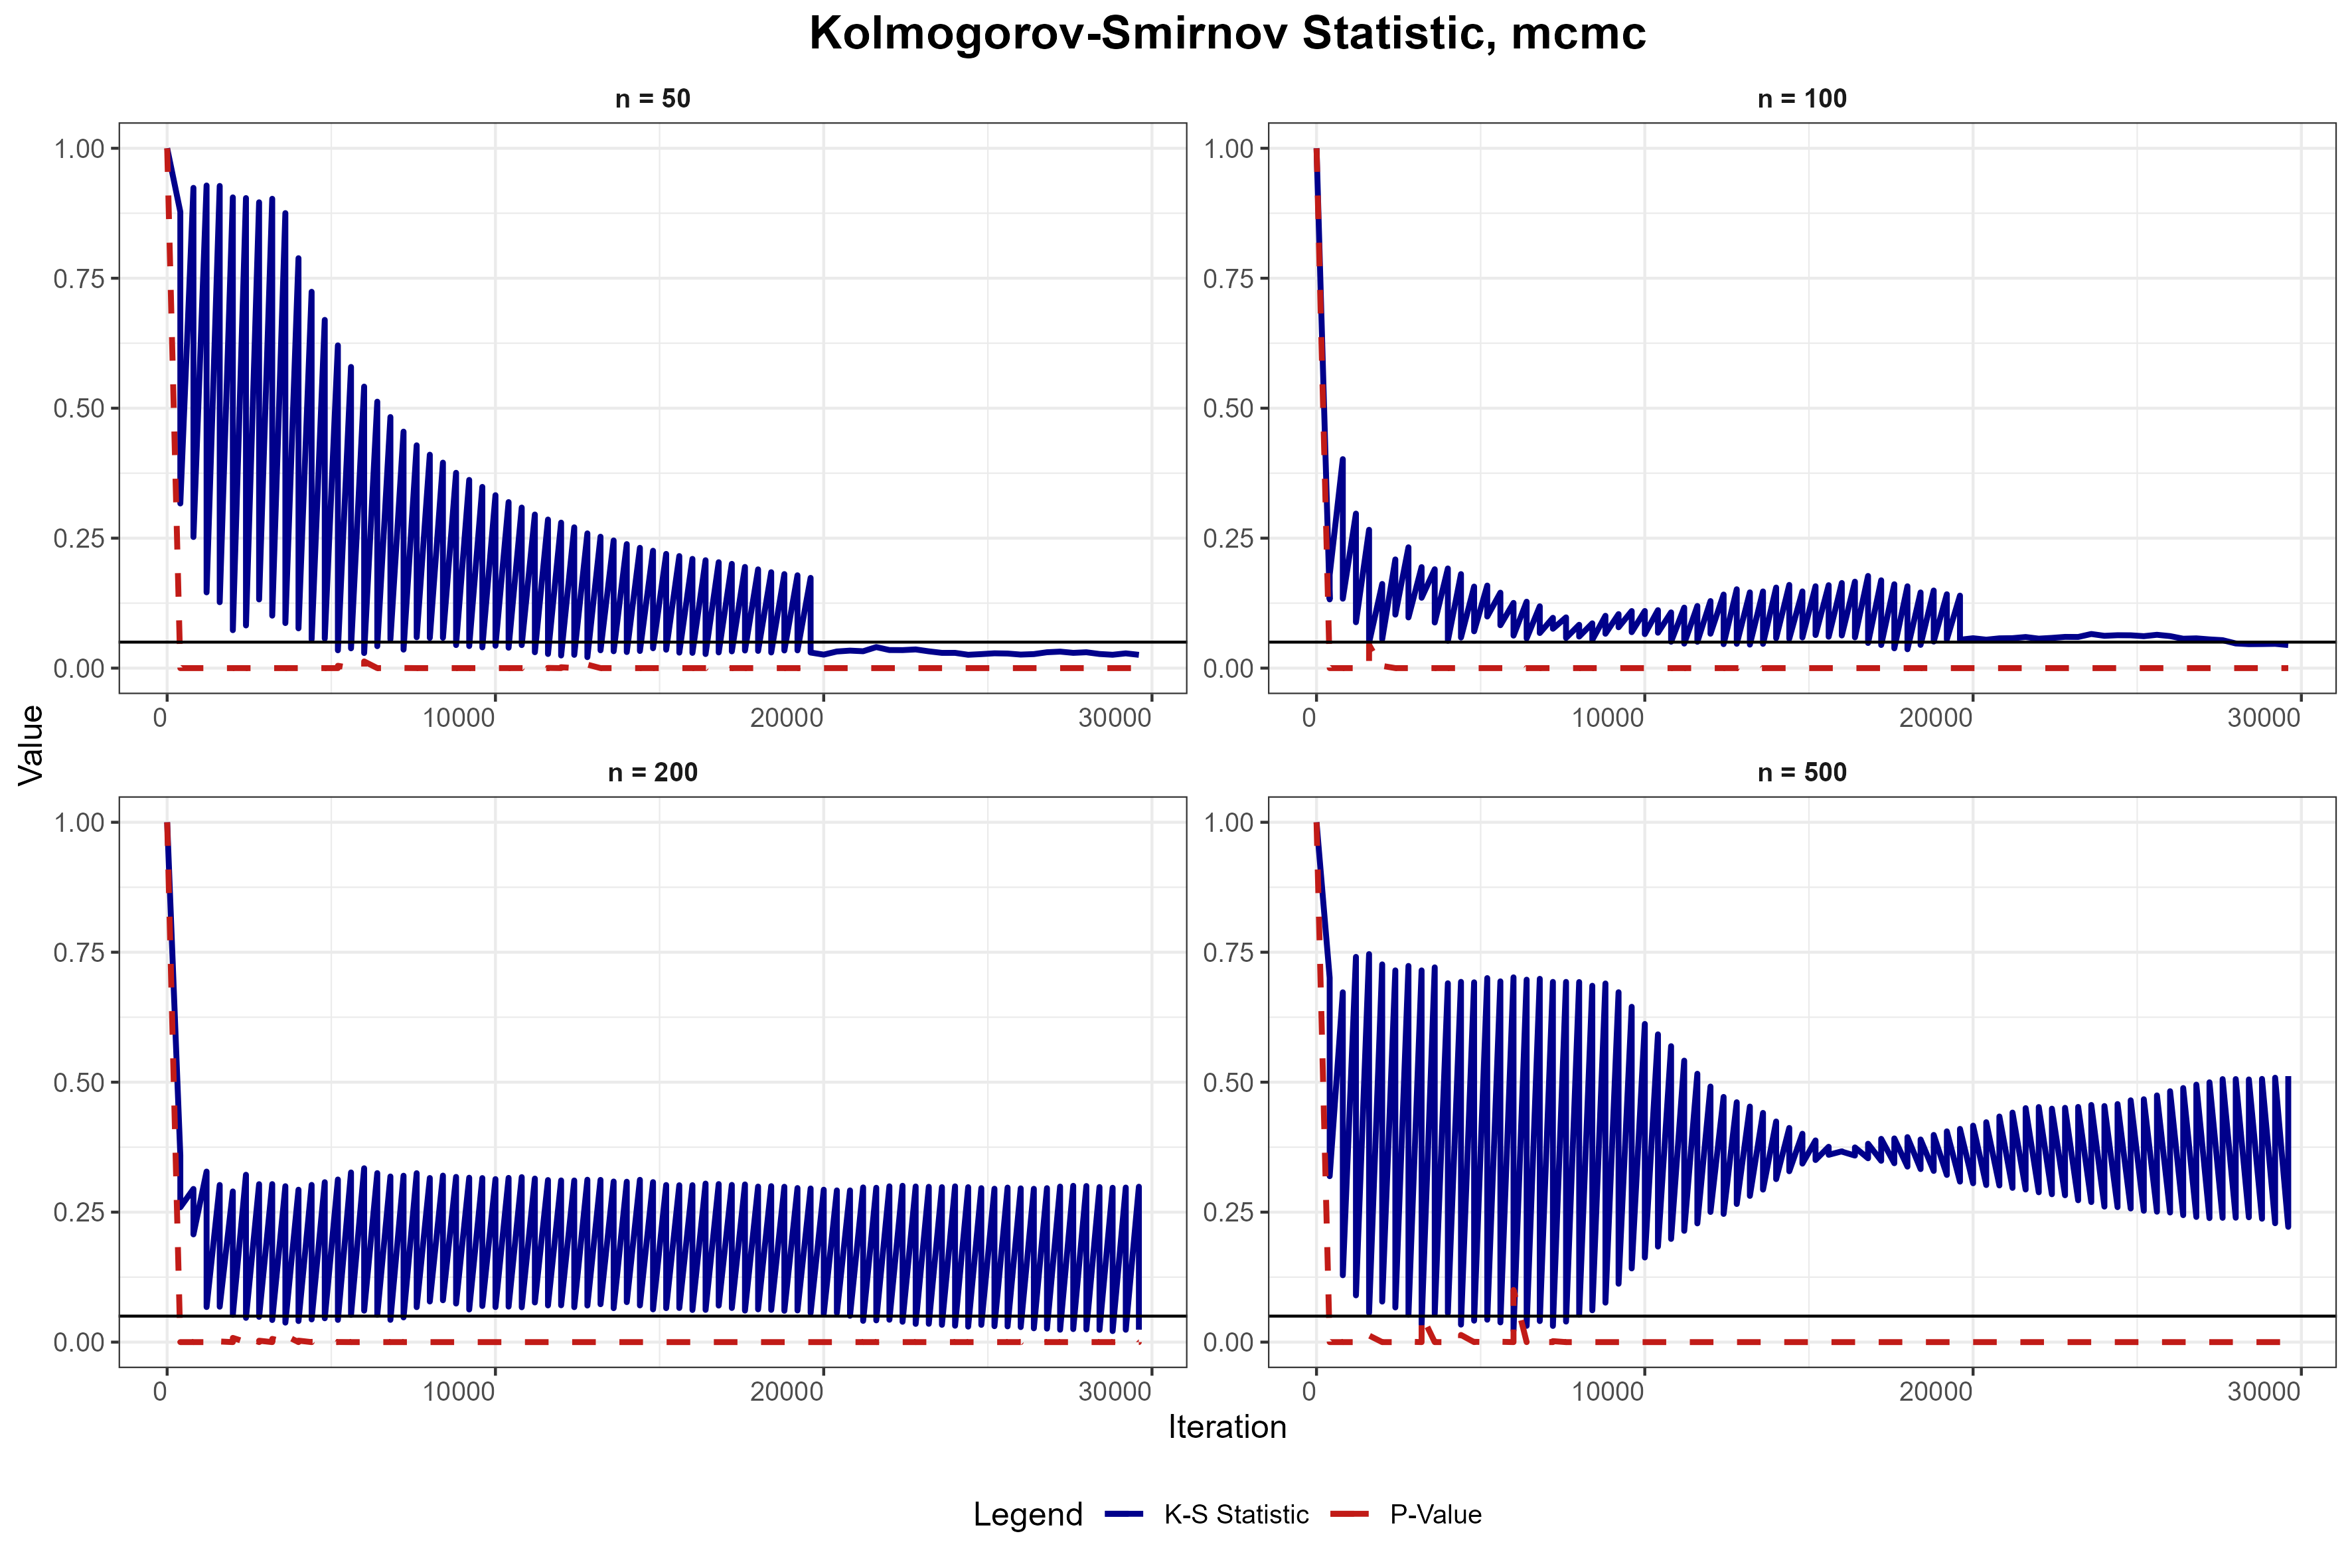
\includegraphics[height=4.1cm]{Figures/Diagnostic/KS_plain_thin.png}
				%\caption{Plain metropolis}
				\label{fig:ks-plain}
			\end{subfigure}
			\hspace{0.35cm}  % horizontal space between figures
			% Second figure
			\begin{subfigure}[b]{0.45\textwidth}   
				\centering
				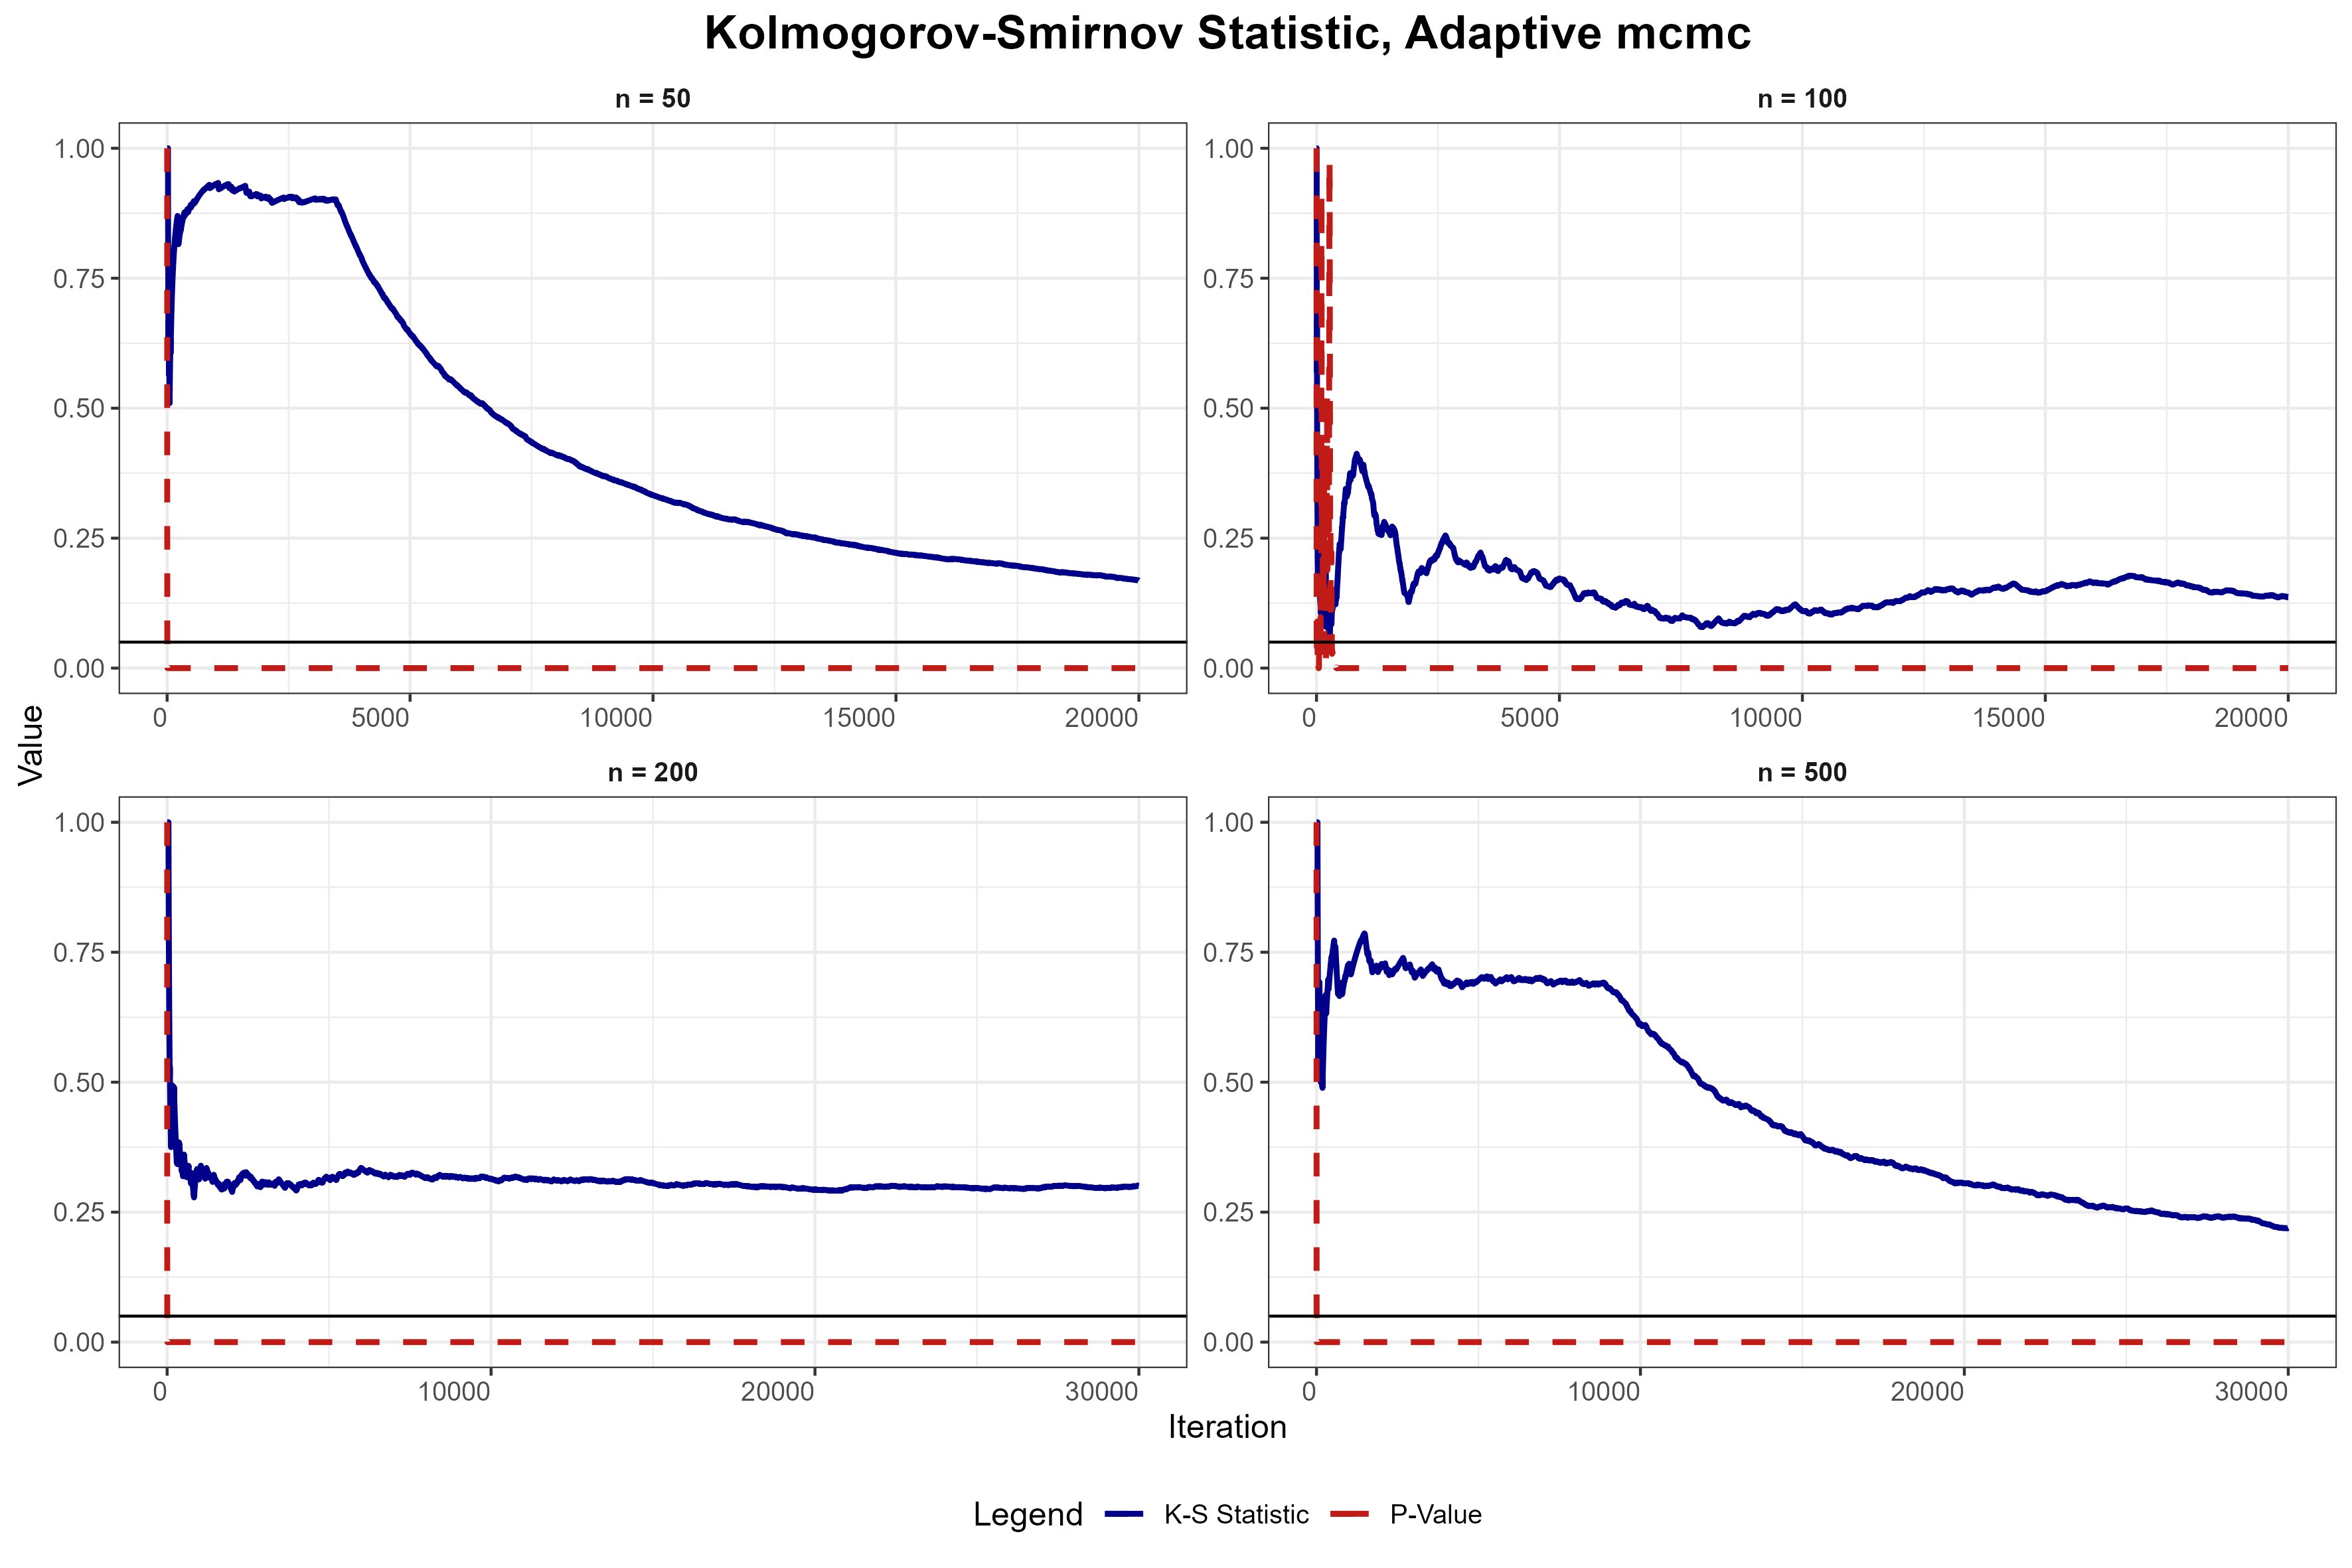
\includegraphics[height=4.1cm]{Figures/Diagnostic/KS_Adaptive.png}
				%\caption{Adaptive metropolis}
				\label{fig:ks-adaptive}
			\end{subfigure}
			
			\vspace{0.4cm}   %  vertical space between rows 
			
			% Third figure
			\begin{subfigure}[b]{0.45\textwidth}   
				\centering
				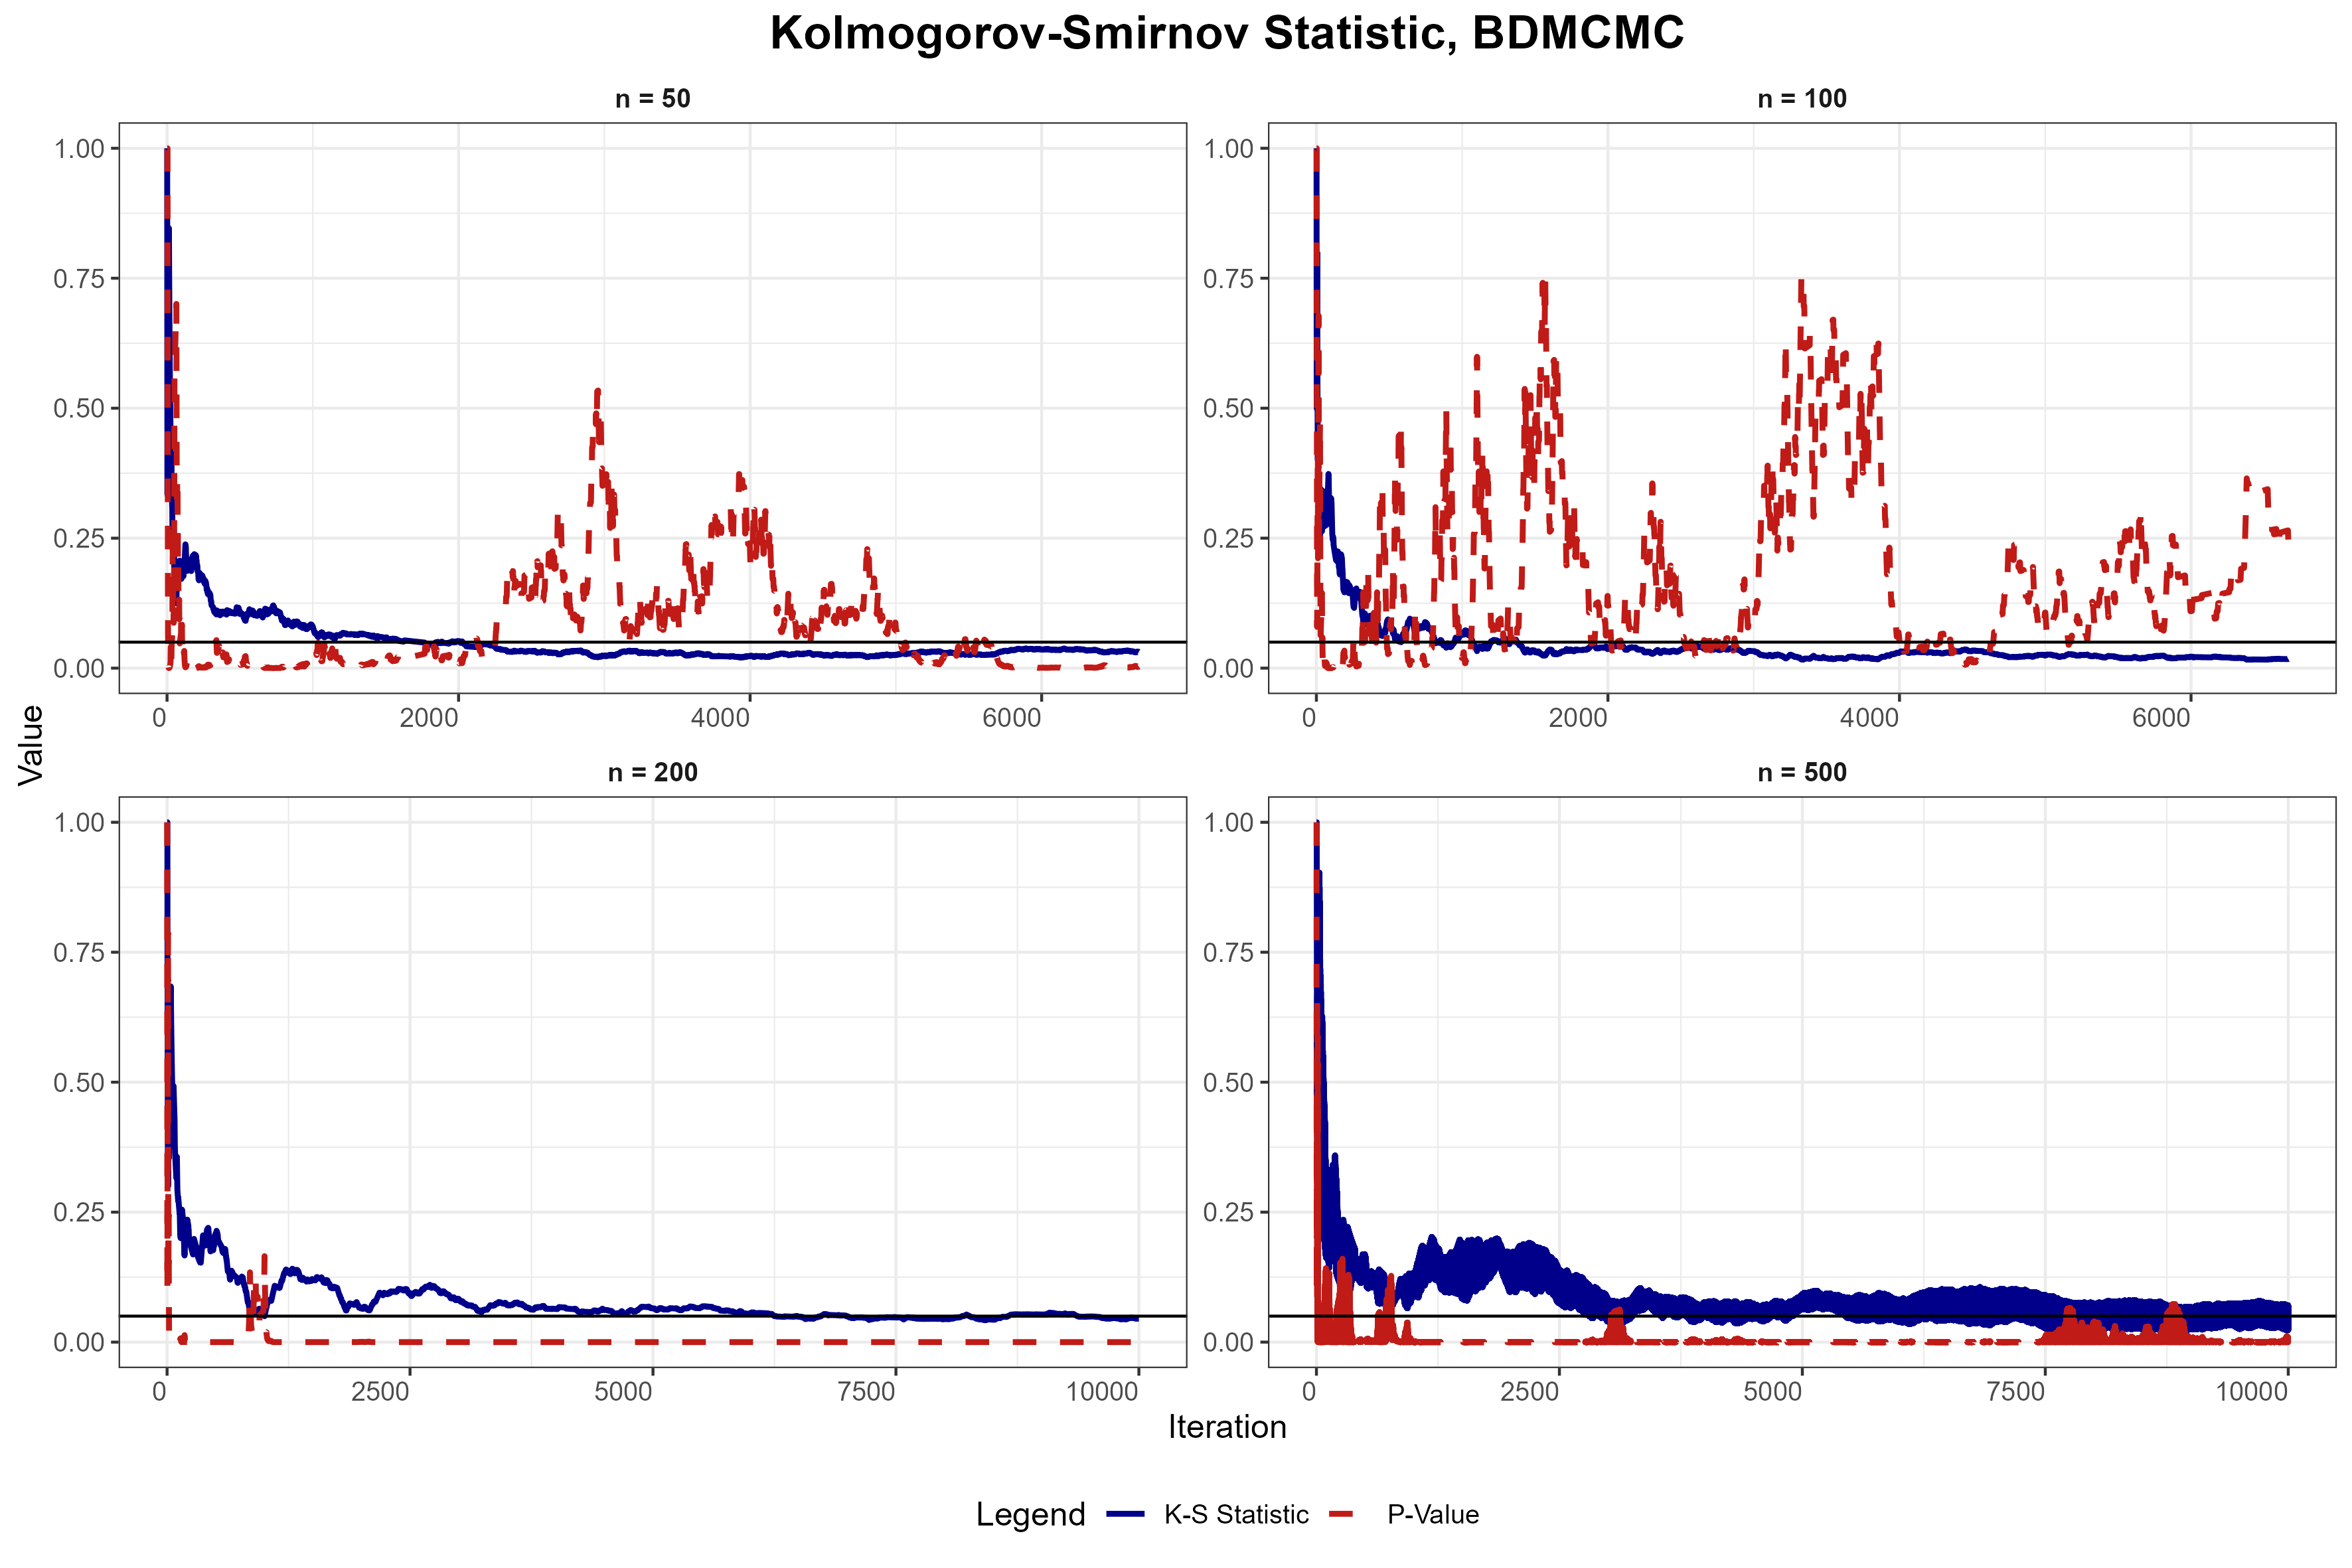
\includegraphics[height=4.1cm]{Figures/Diagnostic/KS_BD.png}
				%\caption{Birth-Death mcmc}
				\label{fig:ks-bd}
			\end{subfigure}
		\end{minipage}
	}
	\caption{Kolmogorov-Smirnov statistic across algorithms. Blue line represents the actual statistic, red line the p-value and black line the 0.05 threshold.}
	\label{fig:ks-together}
\end{figure}

As it can be seen in \ref{fig:ks-together}, the results of the Kolmogorov-Smirnov test illustrate distinct patterns in the stability of the three MCMC algorithms when comparing replicates within each method. For the adaptive MCMC, the test statistic shows a consistent decline across iterations, while the p-value remains below 0.05, indicating a degree of convergence among the replicates. This stability suggests that, although the distributions of samples from different runs are not identical, they become increasingly similar as iterations progress. 

In contrast, when examining the plain MCMC, fluctuations in the test statistic are evident, with values jumping significantly between iterations. Although the p-value consistently remains below 0.05, this variability signals that the replicates are not converging effectively, raising concerns about the overall stability of the algorithm. Notably, at smaller sample sizes (e.g., $n=50$), there is a trend of decreasing test statistics, but this pattern becomes less pronounced as sample size increases. 
Conversely, for the BDMCMC, the test statistic is relatively low for smaller sample sizes (e.g., $n=50$ and $n=100$), resulting in a p-value above 0.05, which suggests that the distributions of the replicates are not significantly different at these iterations. However, as the sample size increases (e.g., $n=200$ and $n=500$), the p-value drops below the threshold, indicating divergence among the replicates. This variability suggests that while the BDMCMC may initially stabilize at smaller sample sizes, it exhibits heightened fluctuations as it explores larger model spaces. Overall, the adaptive MCMC demonstrates greater consistency and stability across its replicates.

\subsection{Structural Hamming Distance (SHD)}

The Structural Hamming Distance is a crucial metric for directly comparing the structure of a learned network to the original network, with a focus primarily on structural discovery rather than inference. SHD is defined as the number of operations needed to make two Partially Directed Acyclic Graphs (PDAGs) identical. These operations include adding or deleting an undirected edge, and adding, removing, or reversing the orientation of an edge. The SHD effectively penalizes algorithms for structural inaccuracies: an increase in SHD by 1 occurs for each additional un-oriented edge in the learned PDAG or for failing to correctly orient an edge that should have been directed (\citet{tsamardinos2006max}).

The Birth-Death algorithm appears to struggle in accurately recovering the true graph structure underlying the data, as evidenced by the substantial errors depicted in \textit{Figure}  \ref{fig:box-shd-bd}. The resulting DAGs are significantly distant from the true configuration, indicating a poor fit. To address these shortcomings, alternative strategies will be explored in the following sections to enhance the algorithm's ability to identify the correct data-generating mechanism.

\begin{figure}[h] 
	\centering
	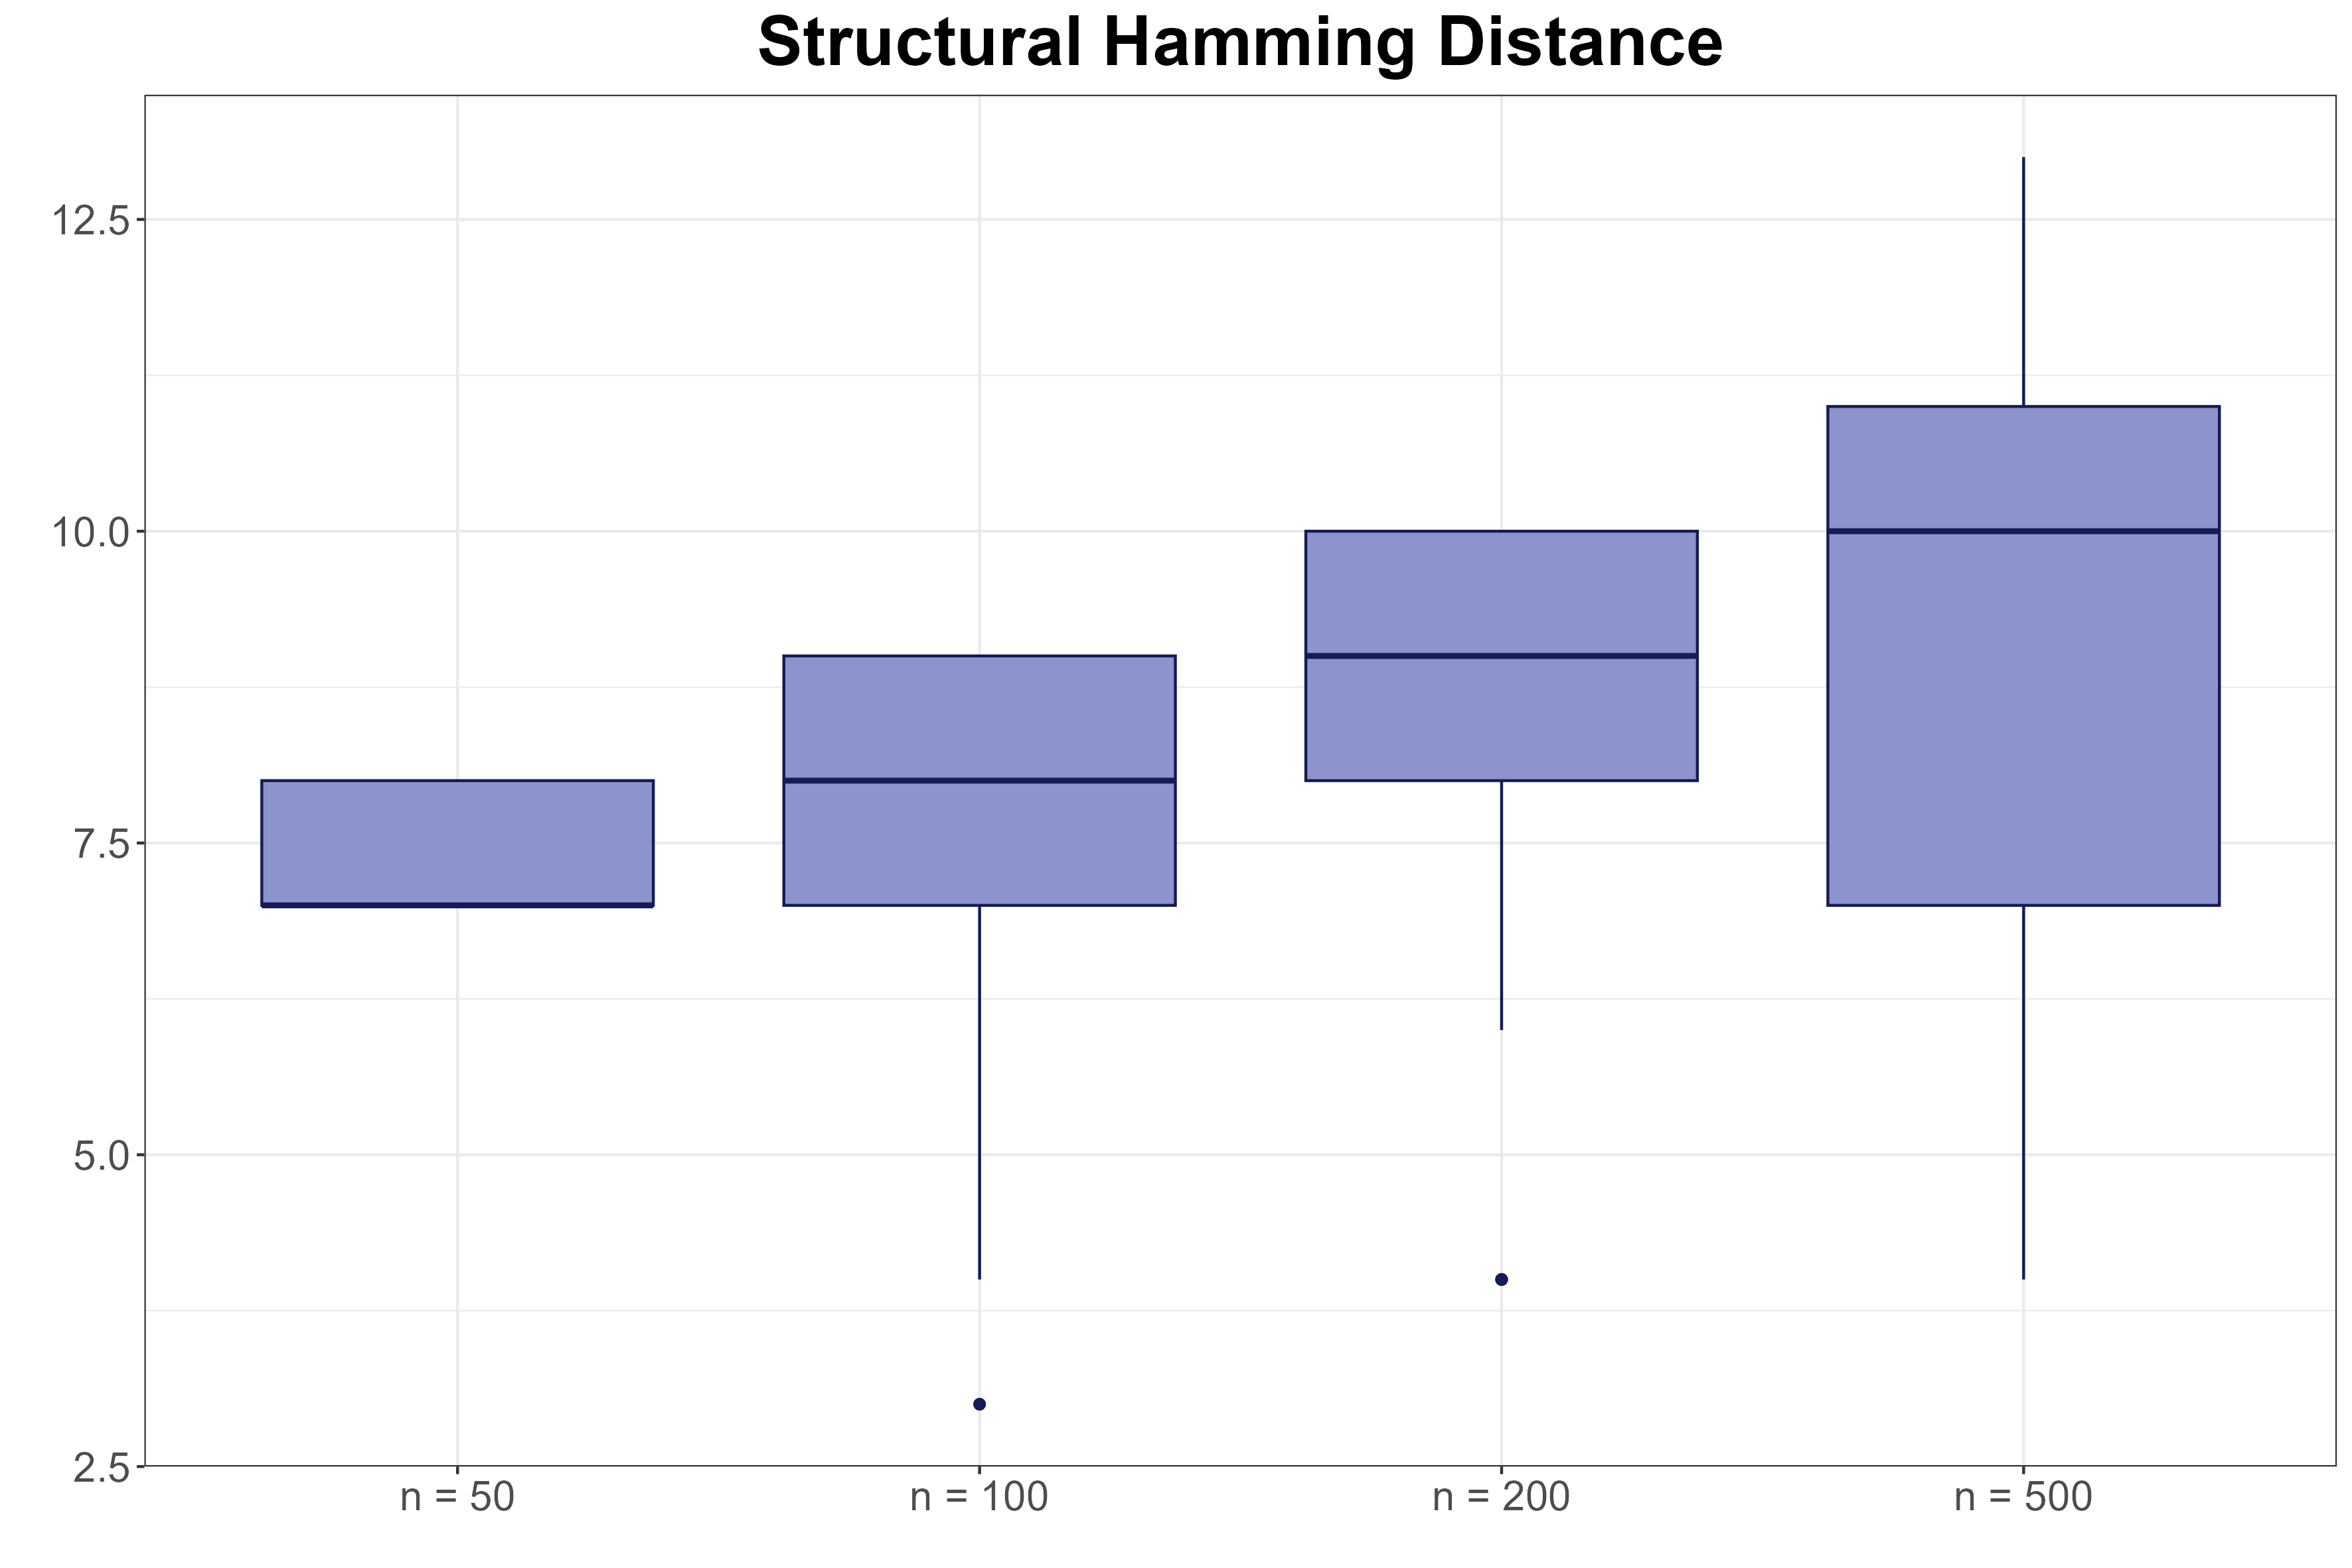
\includegraphics[width=0.6\textwidth]{Figures/Overall_comparison/Boxplot_shd_original.png}
	\caption{Structural hamming distance for different sample sizes}
	\label{fig:box-shd-bd}
\end{figure}

\chapter{Enhancements to Birth-Death MCMC Models}

\section{Refined BDMCMC Code}

Local moves typically involve small, incremental changes to the model, such as adding or removing a single edge in a directed acyclic graph. While these moves are effective in thoroughly exploring the local structure of the model, they can limit the ability to efficiently explore the broader model space. 
To potentially enhance the algorithm's capacity to detect the correct edges and improve convergence, a new global move mechanism is introduced in the BDMCMC framework (\citet{scott2008feature}). This global move aims to perform larger modifications by simultaneously proposing multiple changes to the graph structure. By allowing the chain to make these broader adjustments, the algorithm may be better equipped to traverse complex regions of the model space, avoiding local minima and achieving more accurate model identification. The effectiveness of this approach will be evaluated in subsequent simulations to assess whether it significantly enhances the detection of the correct edges and improves the overall performance.

The code is designed to balance between exploring local modifications and implementing global changes to the DAG. The process begins with a randomly initialized DAG, followed by iterative updates through a series of specialized functions. These functions work together to refine the DAG structure. The first one performs changes within the local neighborhood of the current DAG whereas the second one explores more significant changes by evaluating multiple edge operations simultaneously. 

The process begins by identifying sets of possible edges that can either be added to or removed from the current DAG. These sets are determined by scanning the adjacency matrix for potential edge addition-deletion. For each potential operation, the function temporarily applies the change to the adjacency matrix, generating a new candidate DAG. It then checks whether this candidate structure remains a valid DAG (i.e., it must not contain any cycles). If the candidate DAG is valid, the function proceeds to compute the log-prior and log-likelihood ratios associated with the proposed change. The log-prior ratio reflects the probability of the operation based on a pre-specified weight $w$, while the log-likelihood ratio evaluates the fit of the candidate edge to the observed data. The sum of these ratios determines the overall probability of the operation being accepted. This probability is adjusted using a softmax function, which scales the probabilities to ensure they sum to 1, making them suitable for stochastic selection. 
The function then uses these computed probabilities to probabilistically select the most likely operation from the set of valid changes. The selected operation is applied to the DAG, updating the graph structure. Additionally, the function calculates the waiting time, which is inversely related to the sum of the exponential of the valid log-probabilities. This metric quantifies the likelihood of the selected operation. 

The function includes a mechanism to detect when the updates have stabilized, indicated by consistent waiting times over several iterations. If the waiting time for a DAG remains stable or decreases over 10 consecutive iterations, or if it remains unchanged for multiple iterations, the loop is terminated early. This mechanism ensures that unnecessary computations are not performed once the DAG has likely reached a stable configuration. 

The global move explores a broader set of possible configurations by generating and evaluating combinations of multiple edge insertions and deletions. This approach allows the algorithm to potentially escape local optima by considering more significant changes in the graph structure.
Here, combinations of multiple edge changes are generated. 
For each of these, the function constructs a new candidate DAG by applying the specified insertions and deletions. The likelihood of each new DAG is assessed by calculating the change in its log-likelihood and log-prior compared to the current DAG. Specifically, the function computes the log-likelihoods of the affected nodes before and after the modifications, and it also accounts for the change in the prior probability of the graph structure. 
Since more than one move is carried out at once the ratio is modified to take this further operation into account. For instance, if two separate modifications are made, impacting nodes A and B, the acceptance ratio would be represented by the following expression:

$$
r_{\mathcal{D'}, \mathcal{D''}}= \frac{m(\mathbf{X}_A \ | \  \mathbf{X}_{pa_{\mathcal{D}'}(A)}, \mathcal{D}')}{m(\mathbf{X}_A \  | \  \mathbf{X}_{pa_{\mathcal{D}}(A)}, \mathcal{D})} \times \frac{p(\mathcal{D}')}{p(\mathcal{D})} \times \frac{m(\mathbf{X}_B \ | \  \mathbf{X}_{pa_{\mathcal{D}''}(B)}, \mathcal{D}'')}{m(\mathbf{X}_B \  | \  \mathbf{X}_{pa_{\mathcal{D}}(B)}, \mathcal{D})} \times \frac{p(\mathcal{D}'')}{p(\mathcal{D})}
$$

In the numerator, the terms correspond to the modified DAGs ($\mathcal{D}'$ and $\mathcal{D}''$), reflecting the likelihoods of observing the data given the updated parent sets, as well as the prior probabilities of the updated structures. In the denominator, the terms are associated with the original DAG ($\mathcal{D}$), providing a baseline for comparison.

This structure arises from the conditional independence of the nodes given their respective parent sets. As a result, the acceptance ratio can be expressed as the product of independent terms for the two nodes. Specifically, the likelihood of observing the data for node $A$ under $\mathcal{D}'$ is compared to that under $\mathcal{D}$, while a similar comparison is performed for node $B$ under $\mathcal{D}''$ and $\mathcal{D}$.

More in general, the log-ratio will become a sum of log marginal likelihoods, specifically for each node where a modification takes place, and log prior probabilities.

Local moves are then applied starting from the top 10 candidate DAGs identified during the global move phase. This approach focuses on fine-tuning these promising configurations by iteratively making smaller, localized adjustments to the graph structure. The process aims to further optimize the DAGs by exploring nearby configurations that might offer improvements. 

If a local move results in a DAG with a higher waiting time than the best global move, the function returns this refined DAG, indicating that the local exploration successfully improved upon the initial broad exploration. Conversely, if the global move already yielded the best configuration, the function returns the DAG obtained from the global move. \hfill \break

This more general BDMCMC process starts by initializing a random DAG and performing initial local updates to refine this starting point. Following this, the function enters an iterative cycle. This cycle involves both broad global moves and detailed local adjustments, with the goal of progressively improving the DAG structure. The process is guided by the principle of maximizing the waiting time, the measure of the stability and likelihood of the DAG. The algorithm terminates either when a satisfactory DAG is found, indicated by a significantly improved waiting time, or when a predefined number of moves have been performed. The final output of the function is the most stable DAG discovered during this process, along with the associated waiting time and the matrices of $L$ and $D$ parameters. 

If the global move, obtained performing 2 consequent operations, results in a superior DAG, characterized by an increased waiting time, it is immediately accepted. Otherwise, the function repeats the process attempting with 3 operations this second time. 
This strategy ensures that the algorithm does not settle prematurely on suboptimal solutions but instead explores a diverse range of potential improvements. 

A significant challenge was encountered related to the algorithm's initialization. The algorithm's performance was notably affected by the possibility of beginnning from a suboptimal DAG structure, which could result in becoming 

This issue arises when the algorithm starts in a poor state space, where subsequent moves—whether local or global—tend to yield inferior configurations. Consequently, this leads to a misleading increase in the waiting time metric, which the algorithm interprets as an indication of having reached an optimal or near-optimal solution. However, in reality, this only reflects a stagnation in a low-quality region of the search space. 
To address this issue, an additional step was introduced at the very beginning of the BDMCMC algorithm. Before initiating the main sampling process, the algorithm now generates 30 random DAG structures. For each of these structures, the associated waiting time is calculated. The DAG with the highest waiting time is then selected as the starting point for subsequent sampling and refinement processes. This approach reduces the risk of starting in a poor state space by enabling a more informed choice of the initial configuration. 

Here is how the $birth\_death$ algorithm is structured:

\begin{algorithm}[H]
	\caption{Birth-Death Process (improved version)}
	\begin{algorithmic}[1]
		\State \textbf{Begin} birth\_death function
		\State \textbf{Initialize} matrices $G$, $D$, and $L$ as empty
		\State \textbf{Generate} 30 initial random DAGs
		\State \textbf{Select} the best DAG based on waiting time
		\State \textbf{Perform} local moves on the initial DAG
		
		\While{maximum number of moves is not reached}
		\State \textbf{Perform} a global move by conducting two operations simultaneously
		\State \textbf{Check} if the global move results in a better DAG compared to the previous one
		
		\If{the global move is better}
		\State \textbf{Update} the DAG and its waiting time
		\Else
		\State \textbf{Try} performing three operations in the global move
		\EndIf
		
		\State \textbf{Add} the new DAG to the third dimension of the $G$ matrix
		\State \textbf{Stop} if the number of moves exceeds the maximum allowed or if no improvement is found
		\EndWhile
		
		\State \textbf{Sample} $L$ and $D$ parameters from the full conditional , the DAG-Wishart distribution
		\State \textbf{Fill} the corresponding matrices
		\State \textbf{Return} the final DAG, associated waiting times, and parameter matrices
		\State \textbf{End} birth\_death function
	\end{algorithmic}
\end{algorithm}

\section{Comparative Performance Analysis}

The goal of this section is to provide a comprehensive evaluation of the performance of four different MCMC algorithms: the plain Metropolis, the adaptive MCMC with two different levels of the tuning parameter C (0.5 and 0.7), and the Birth-Death MCMC. The comparison is based on the ability of each algorithm to correctly identify the true underlying graph structure and accurately detect significant edges. To ensure consistency and fairness in the evaluation, the same true graph structure is used across all simulations.

Several performance metrics are employed to quantify the effectiveness of each algorithm, including True Positives, True Negatives, False Positives, and False Negatives. These metrics will be used to calculate derived measures such as F-score, Accuracy, and the Matthews Correlation Coefficient,. Additionally, the Kullback-Leibler divergence of both parameters $L$ and the $D$ will be computed to assess how well the algorithms capture the overall distribution of the graphs.
Visual comparisons will be presented through heatmaps of the estimated edge inclusion probabilities, highlighting which edges are consistently assigned a higher probability mass by each algorithm. Further, to evaluate the overall similarity between the sampled and true graph structures, the Structural Hamming Distance (SHD) will be used. This metric provides a measure of the discrepancy between the estimated and true graphs, summarizing the accuracy of the entire structure.

In MCMC methods, the selected DAG is determined using the Median Probability Model (MPM) approach, which involves including all edges $u \rightarrow v$ whose estimated probability of inclusion is greater than 0.5. This threshold ensures that only the edges that are more likely to exist than not are incorporated, providing a balance between sensitivity and specificity in identifying significant connections. In contrast, the BDMCMC method selects the DAG that exhibits the highest waiting time during the sampling process. A higher waiting time indicates that the algorithm finds it challenging to transition away from this configuration, suggesting that the corresponding structure has a high posterior probability and represents a well-supported solution.

\subsection{Posterior probability}

The posterior probability of edge inclusion is illustrated in \textit{Figure} \ref{fig:four-heatmaps}. The results indicate that as the sample size increases, the accuracy of edge detection improves. Specifically, with a sample size of 50, all four algorithms can only identify the three most prominent dependencies. However, with sample sizes of 100 and 200, the BDMCMC algorithm demonstrates superior performance in identifying significant edges, as it is the only method that assigns a higher probability mass to the correct edges.

It is noteworthy that the three Metropolis-based algorithms exhibit similar behavior, whereas the BDMCMC algorithm shows distinct differences. This discrepancy arises from the differing methodologies employed by the algorithms in edge selection. The Metropolis algorithms derive edge probabilities based on the average inclusion or exclusion of edges over sixty thousand samples. This high number of samples contributes to convergence and results in similar edge probabilities across these algorithms.

In contrast, the BDMCMC algorithm operates differently. It samples a relatively smaller number of DAGs; less than 60 on average per execution, as shown in \textit{Figure} \ref{fig:n-dags}. For each DAG, BDMCMC evaluates all possible edge inclusions or deletions based on log-likelihood and log-prior probability.

\begin{figure}[!ht]
	\centering
	\resizebox{\textwidth}{6.5cm}{  
		\begin{minipage}{\textwidth}
			\centering
			
			% First figure
			\begin{subfigure}[b]{0.45\textwidth}   
				\centering
				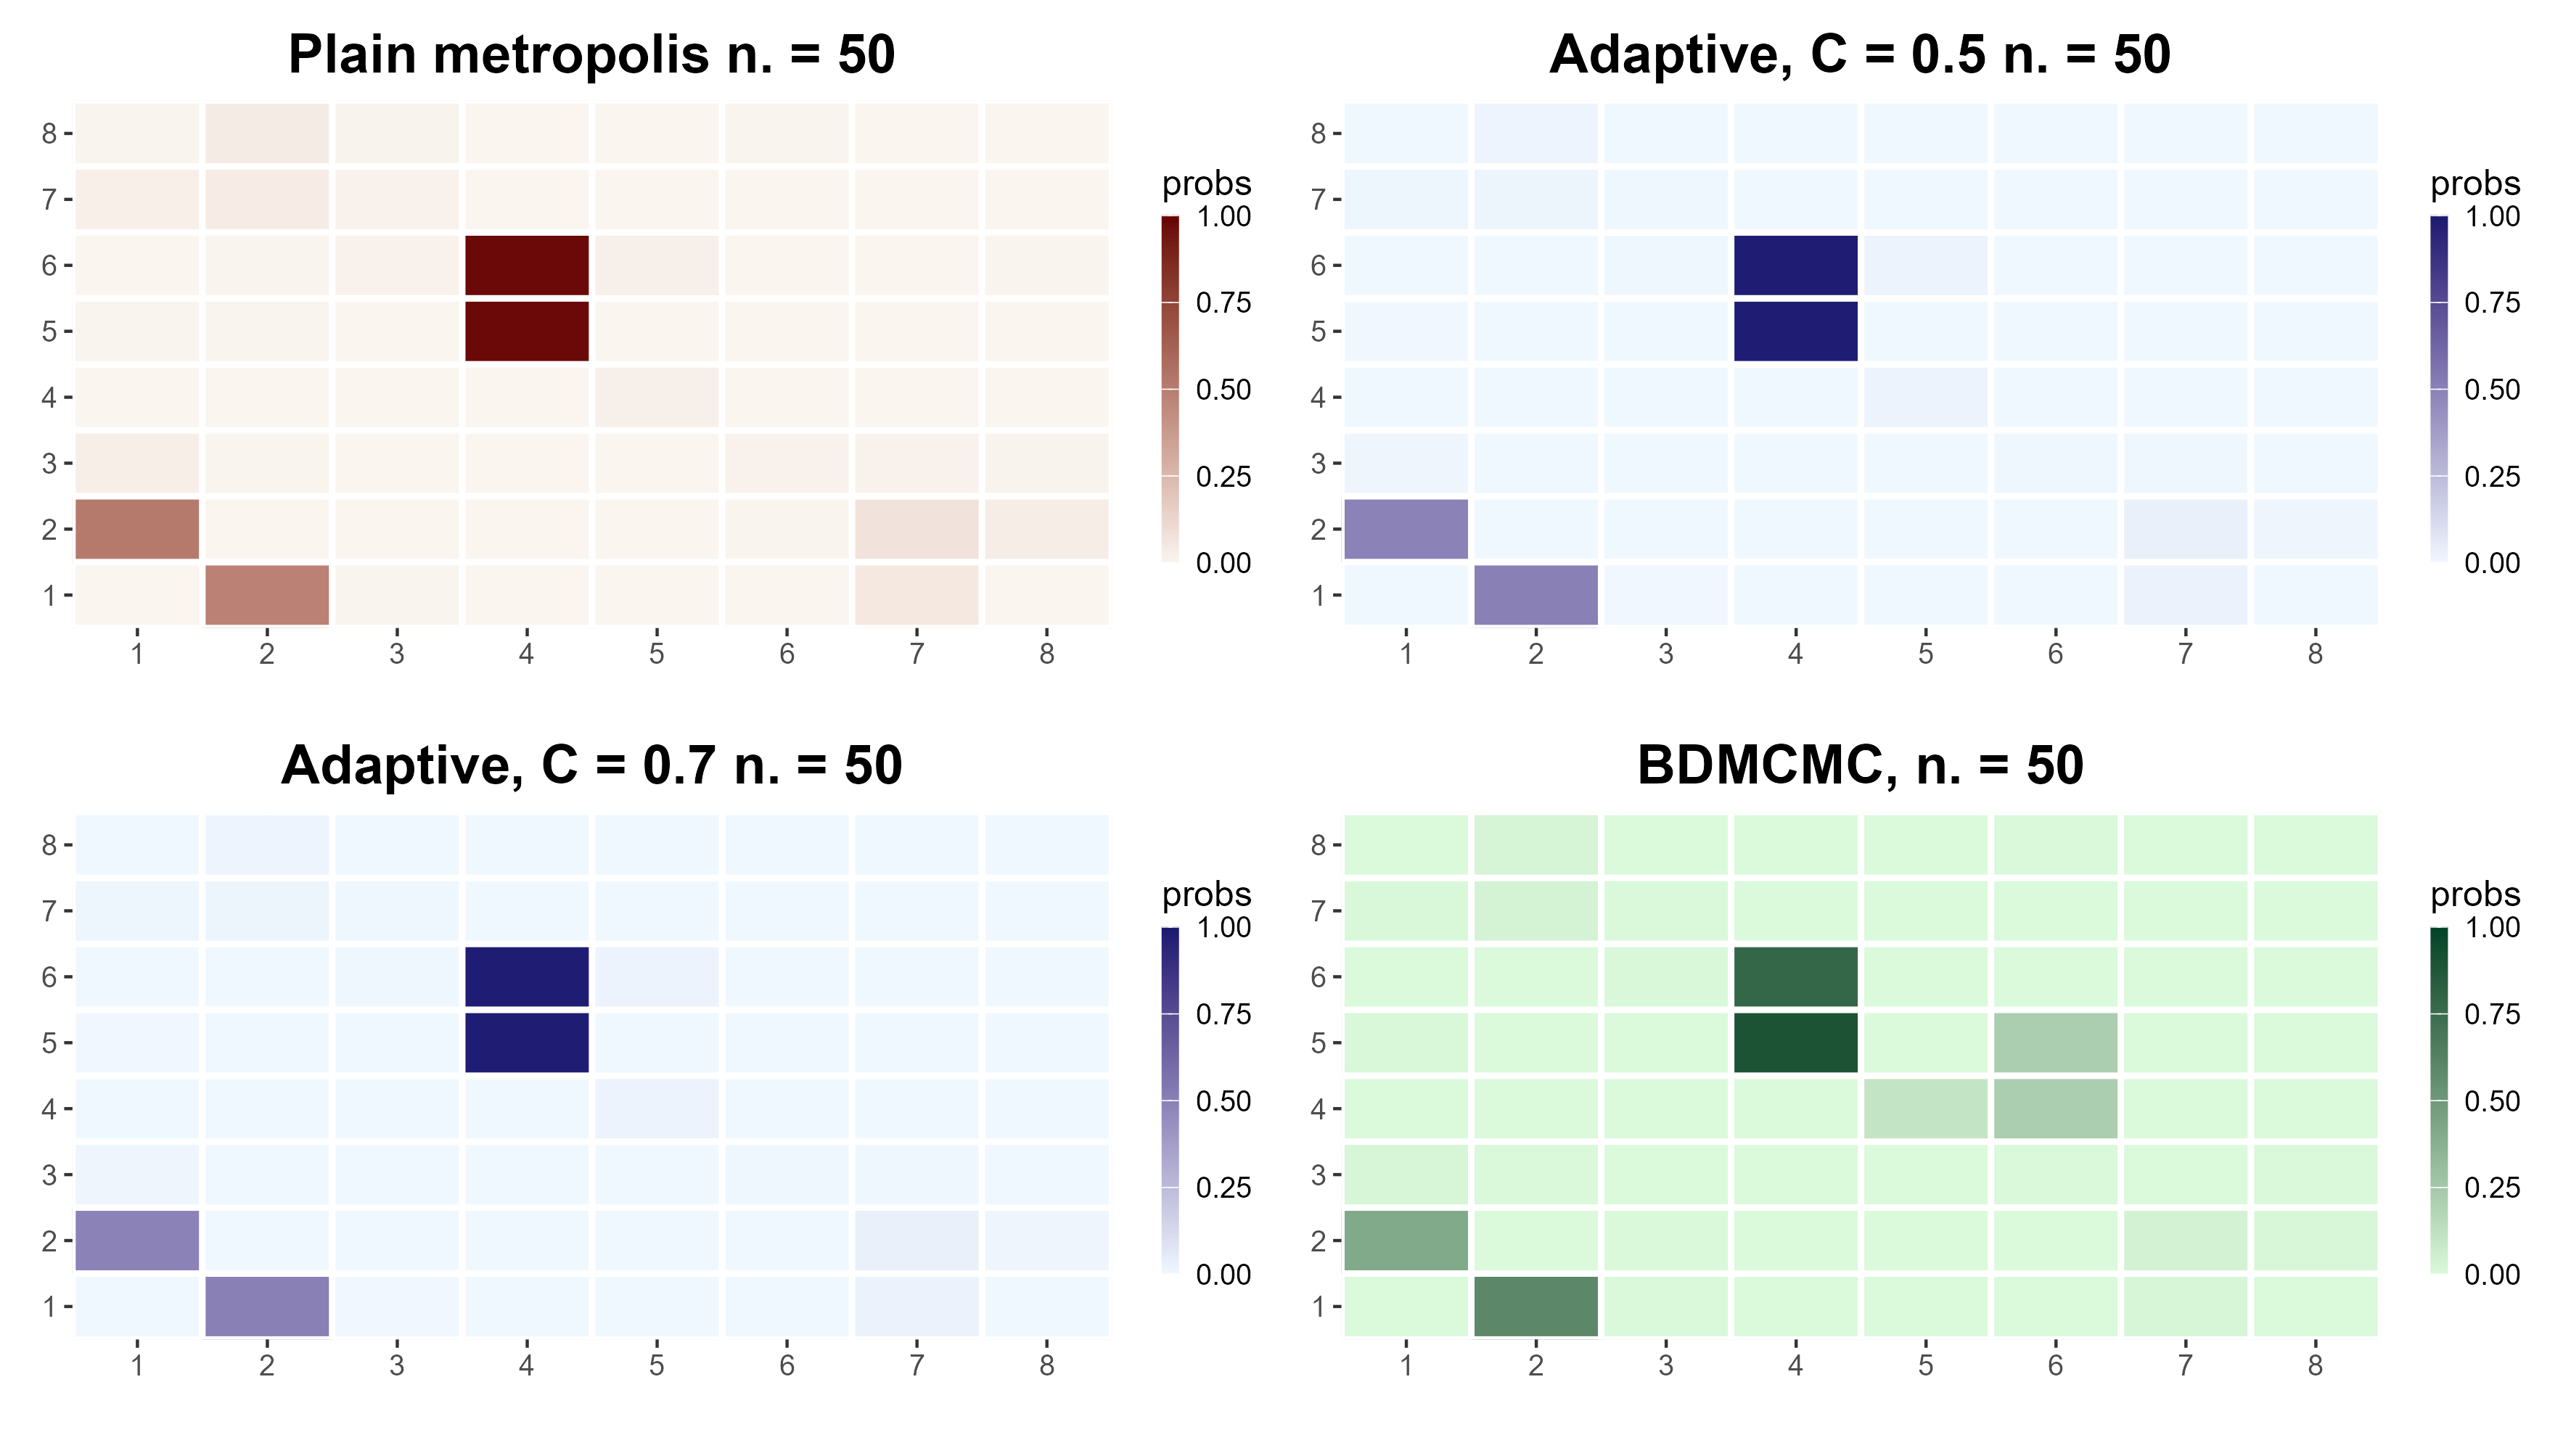
\includegraphics[height=4.1cm]{Figures/Overall_comparison/n50_heatmaps.png}
				%\caption{Sample size 50}
				\label{fig:heatmaps-50}
			\end{subfigure}
			\hspace{0.35cm}  % horizontal space between figures
			% Second figure
			\begin{subfigure}[b]{0.45\textwidth}   
				\centering
				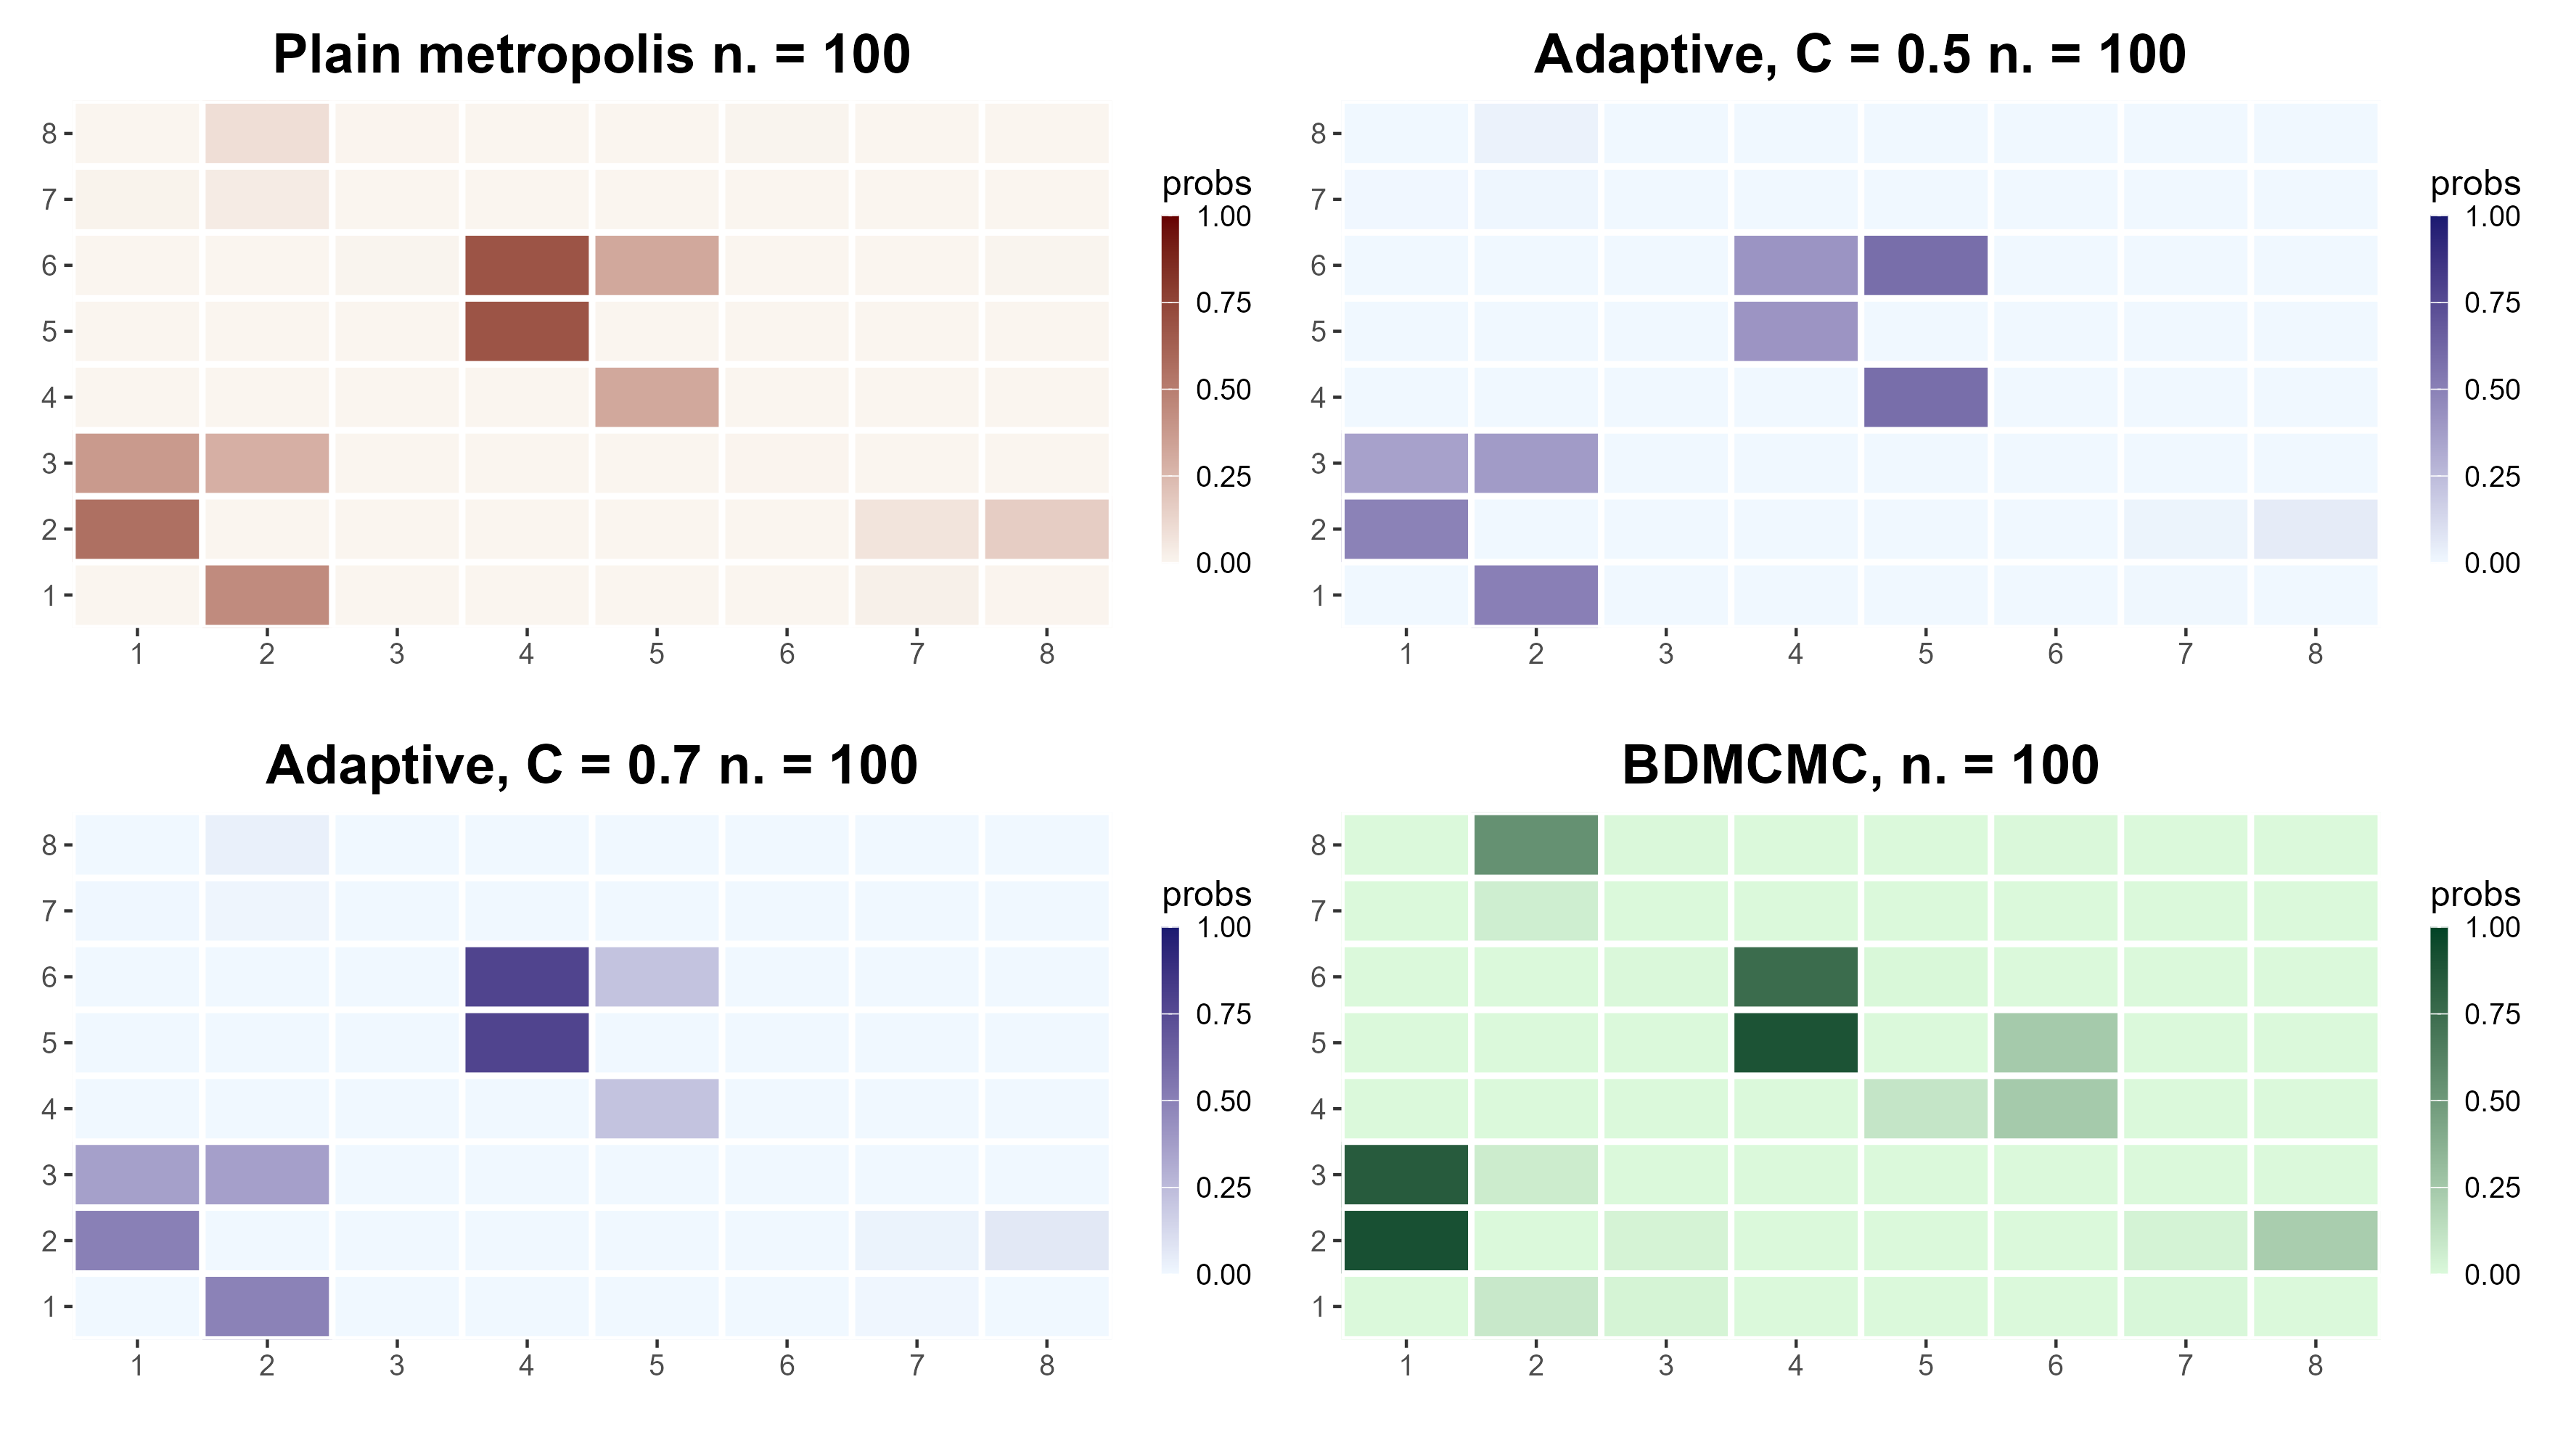
\includegraphics[height=4.1cm]{Figures/Overall_comparison/n100_heatmaps.png}
				%\caption{Sample size 100}
				\label{fig:heatmaps-100}
			\end{subfigure}
			
			\vspace{0.4cm}   %  vertical space between rows 
			
			% Third figure
			\begin{subfigure}[b]{0.45\textwidth}   
				\centering
				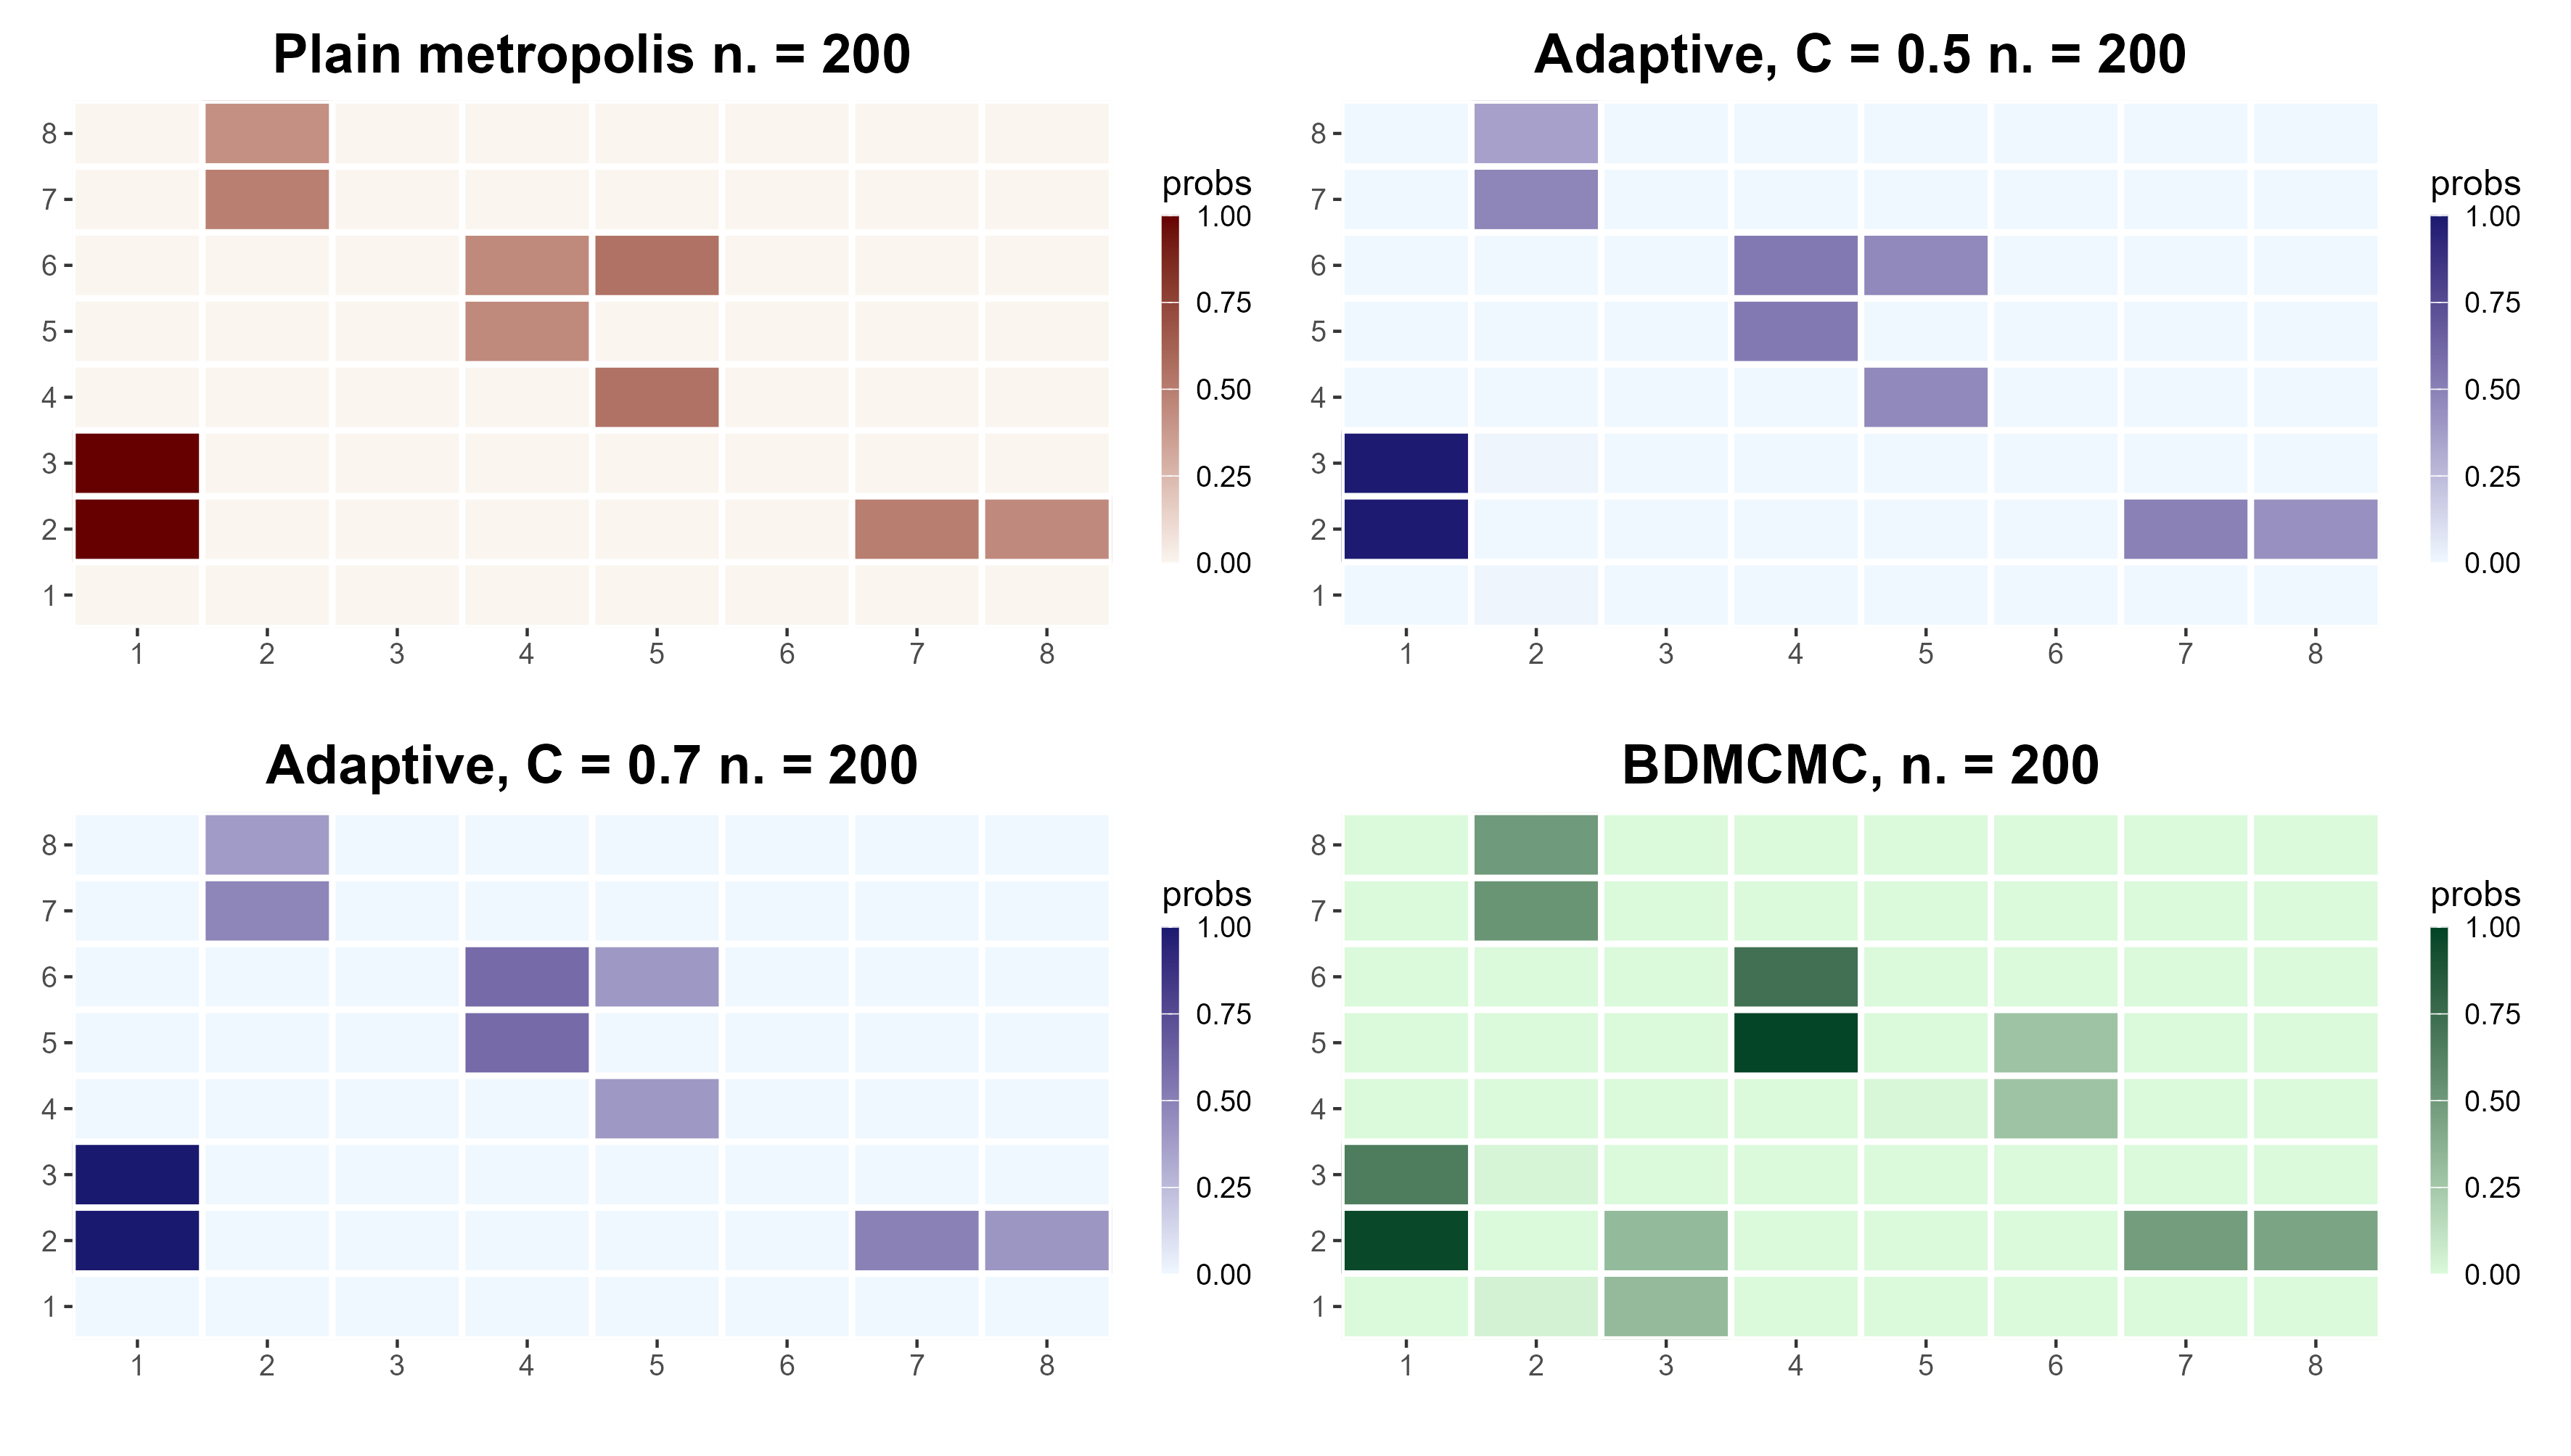
\includegraphics[height=4.1cm]{Figures/Overall_comparison/n200_heatmaps.png}
				%\caption{Sample size 200}
				\label{fig:heatmaps-200}
			\end{subfigure}
			\hspace{0.35cm}  % horizontal space between figures
			% Fourth figure
			\begin{subfigure}[b]{0.45\textwidth}   
				\centering
				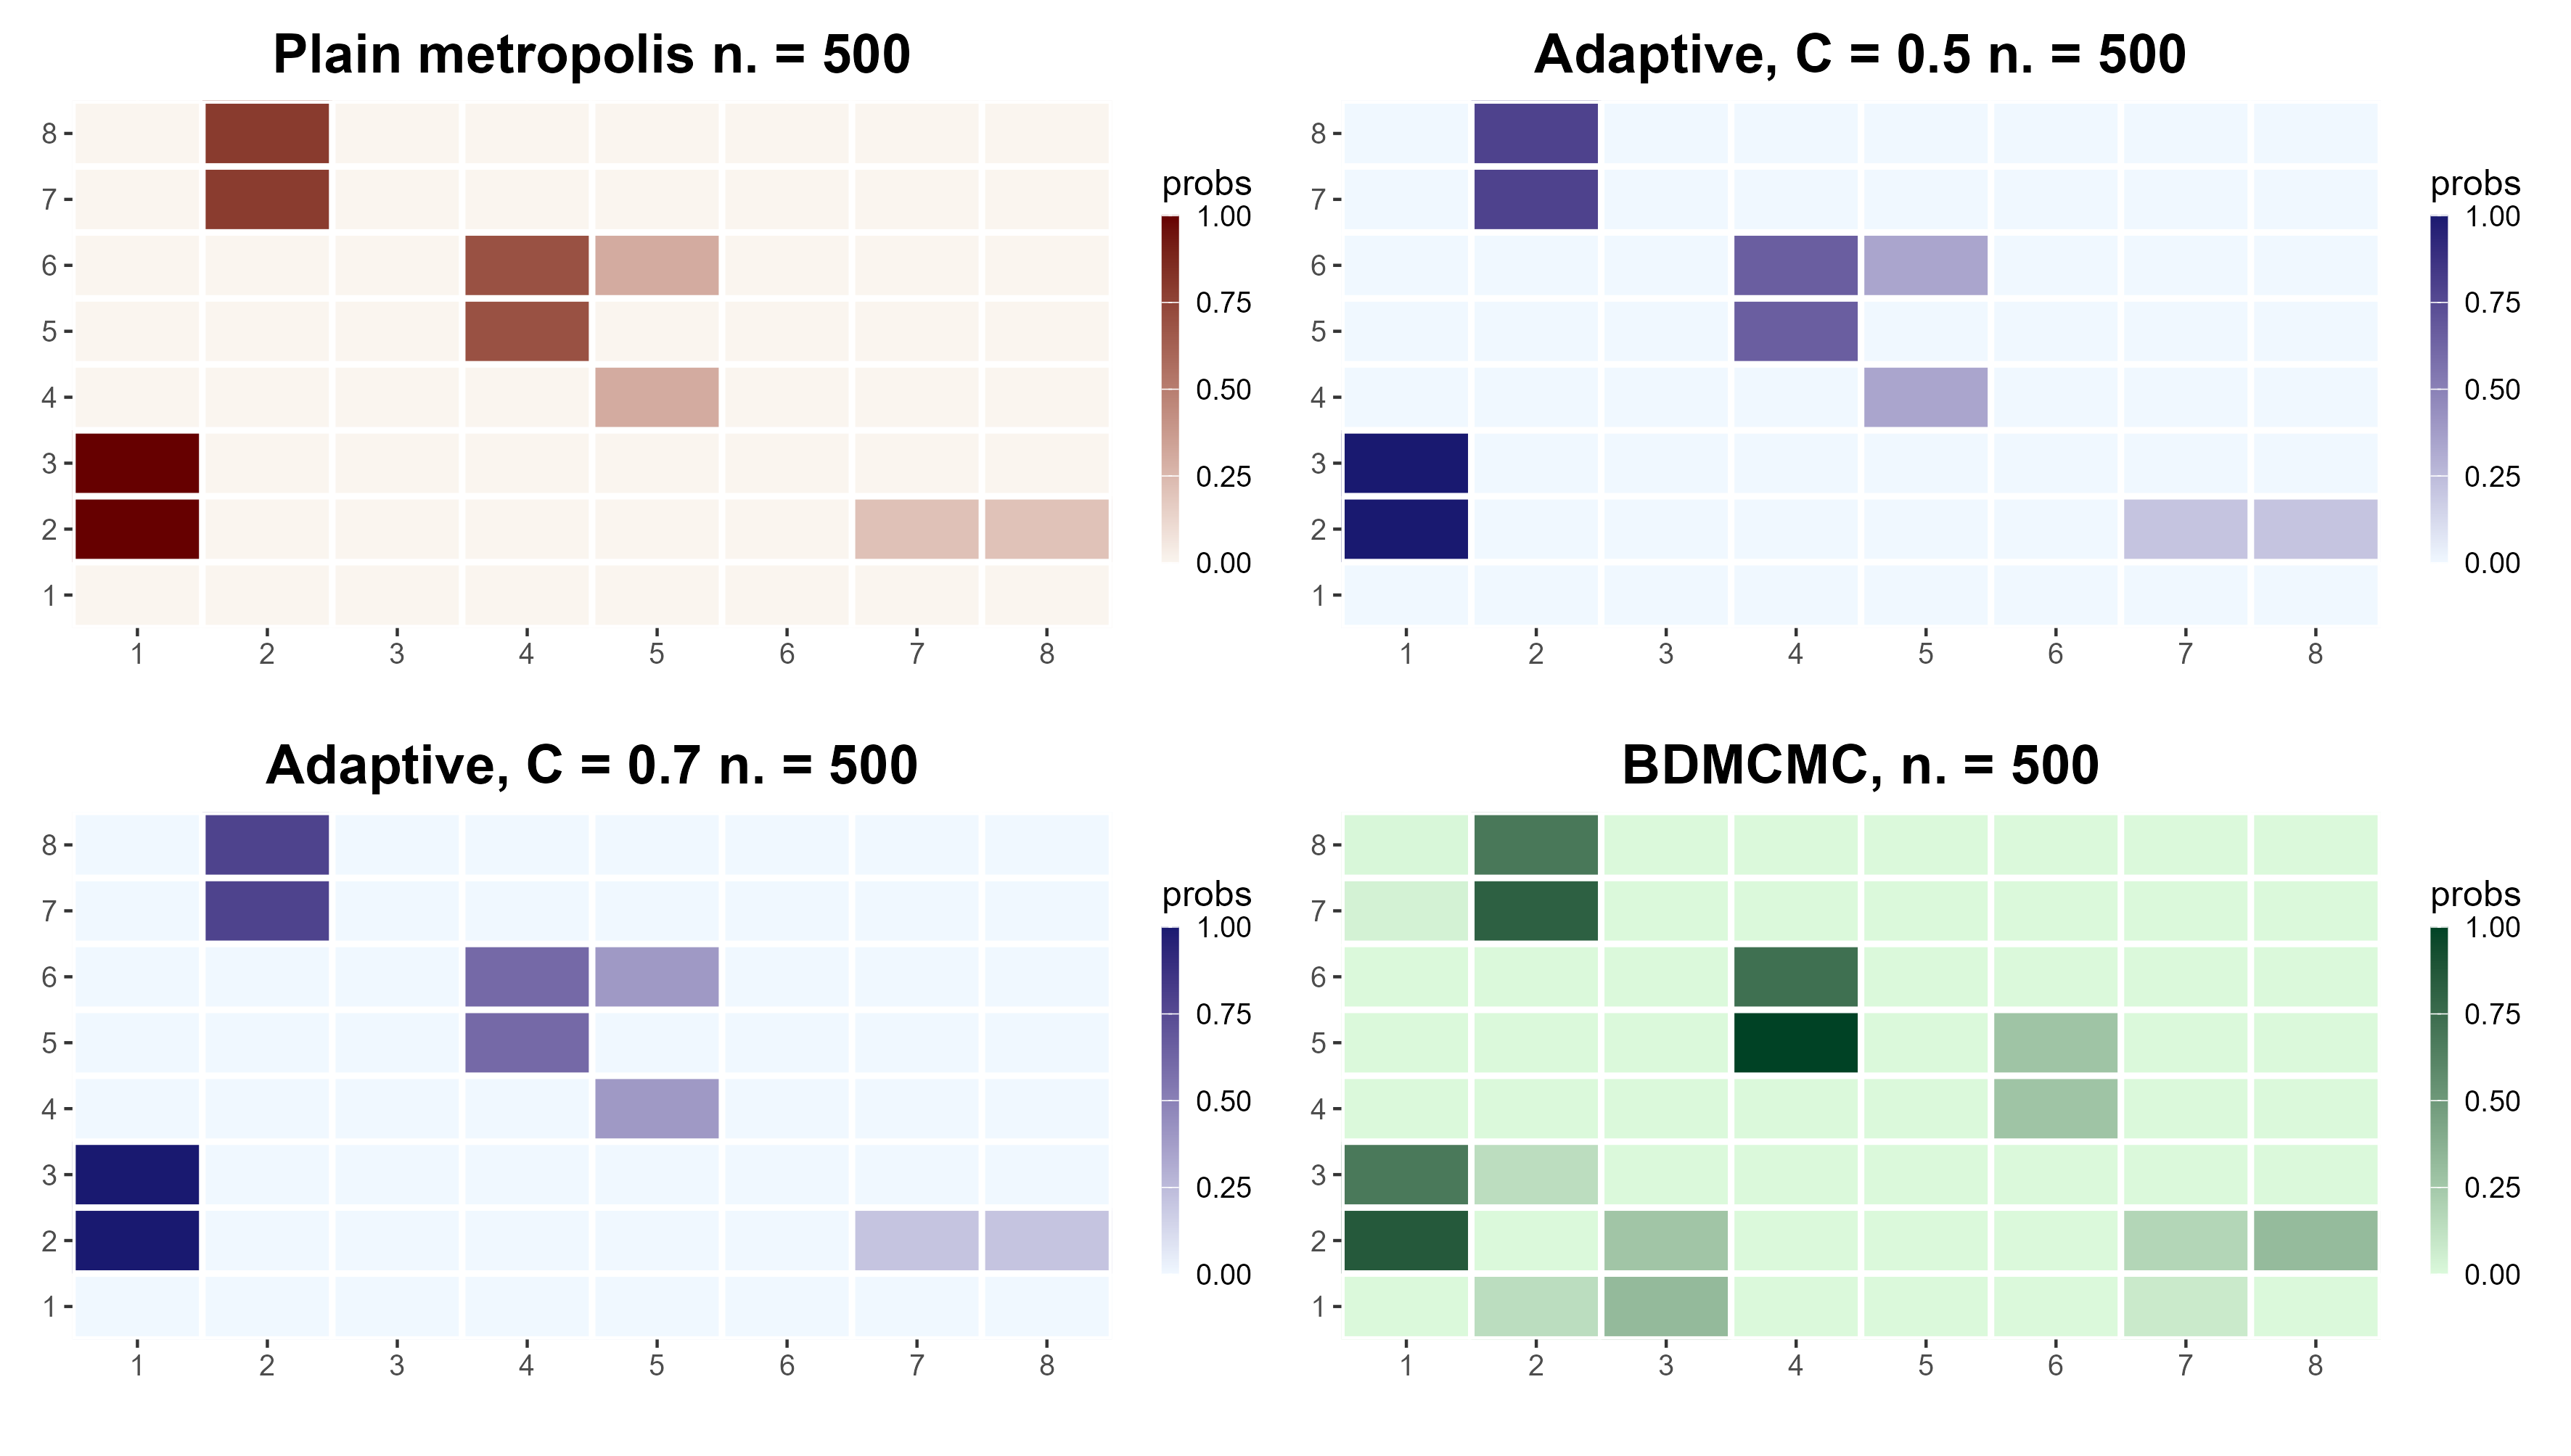
\includegraphics[height=4.1cm]{Figures/Overall_comparison/n500_heatmaps.png}
				%\caption{Sample size 500}
				\label{fig:heatmaps-500}
			\end{subfigure}
		\end{minipage}
	}
	\caption{Heatmaps illustrating the edge inclusion probability across different numerosities, with final estimates computed as the mean probability of inclusion across 15 replicates for each algorithm.}
	\label{fig:four-heatmaps}
\end{figure}

\begin{figure}[h] 
	\centering
	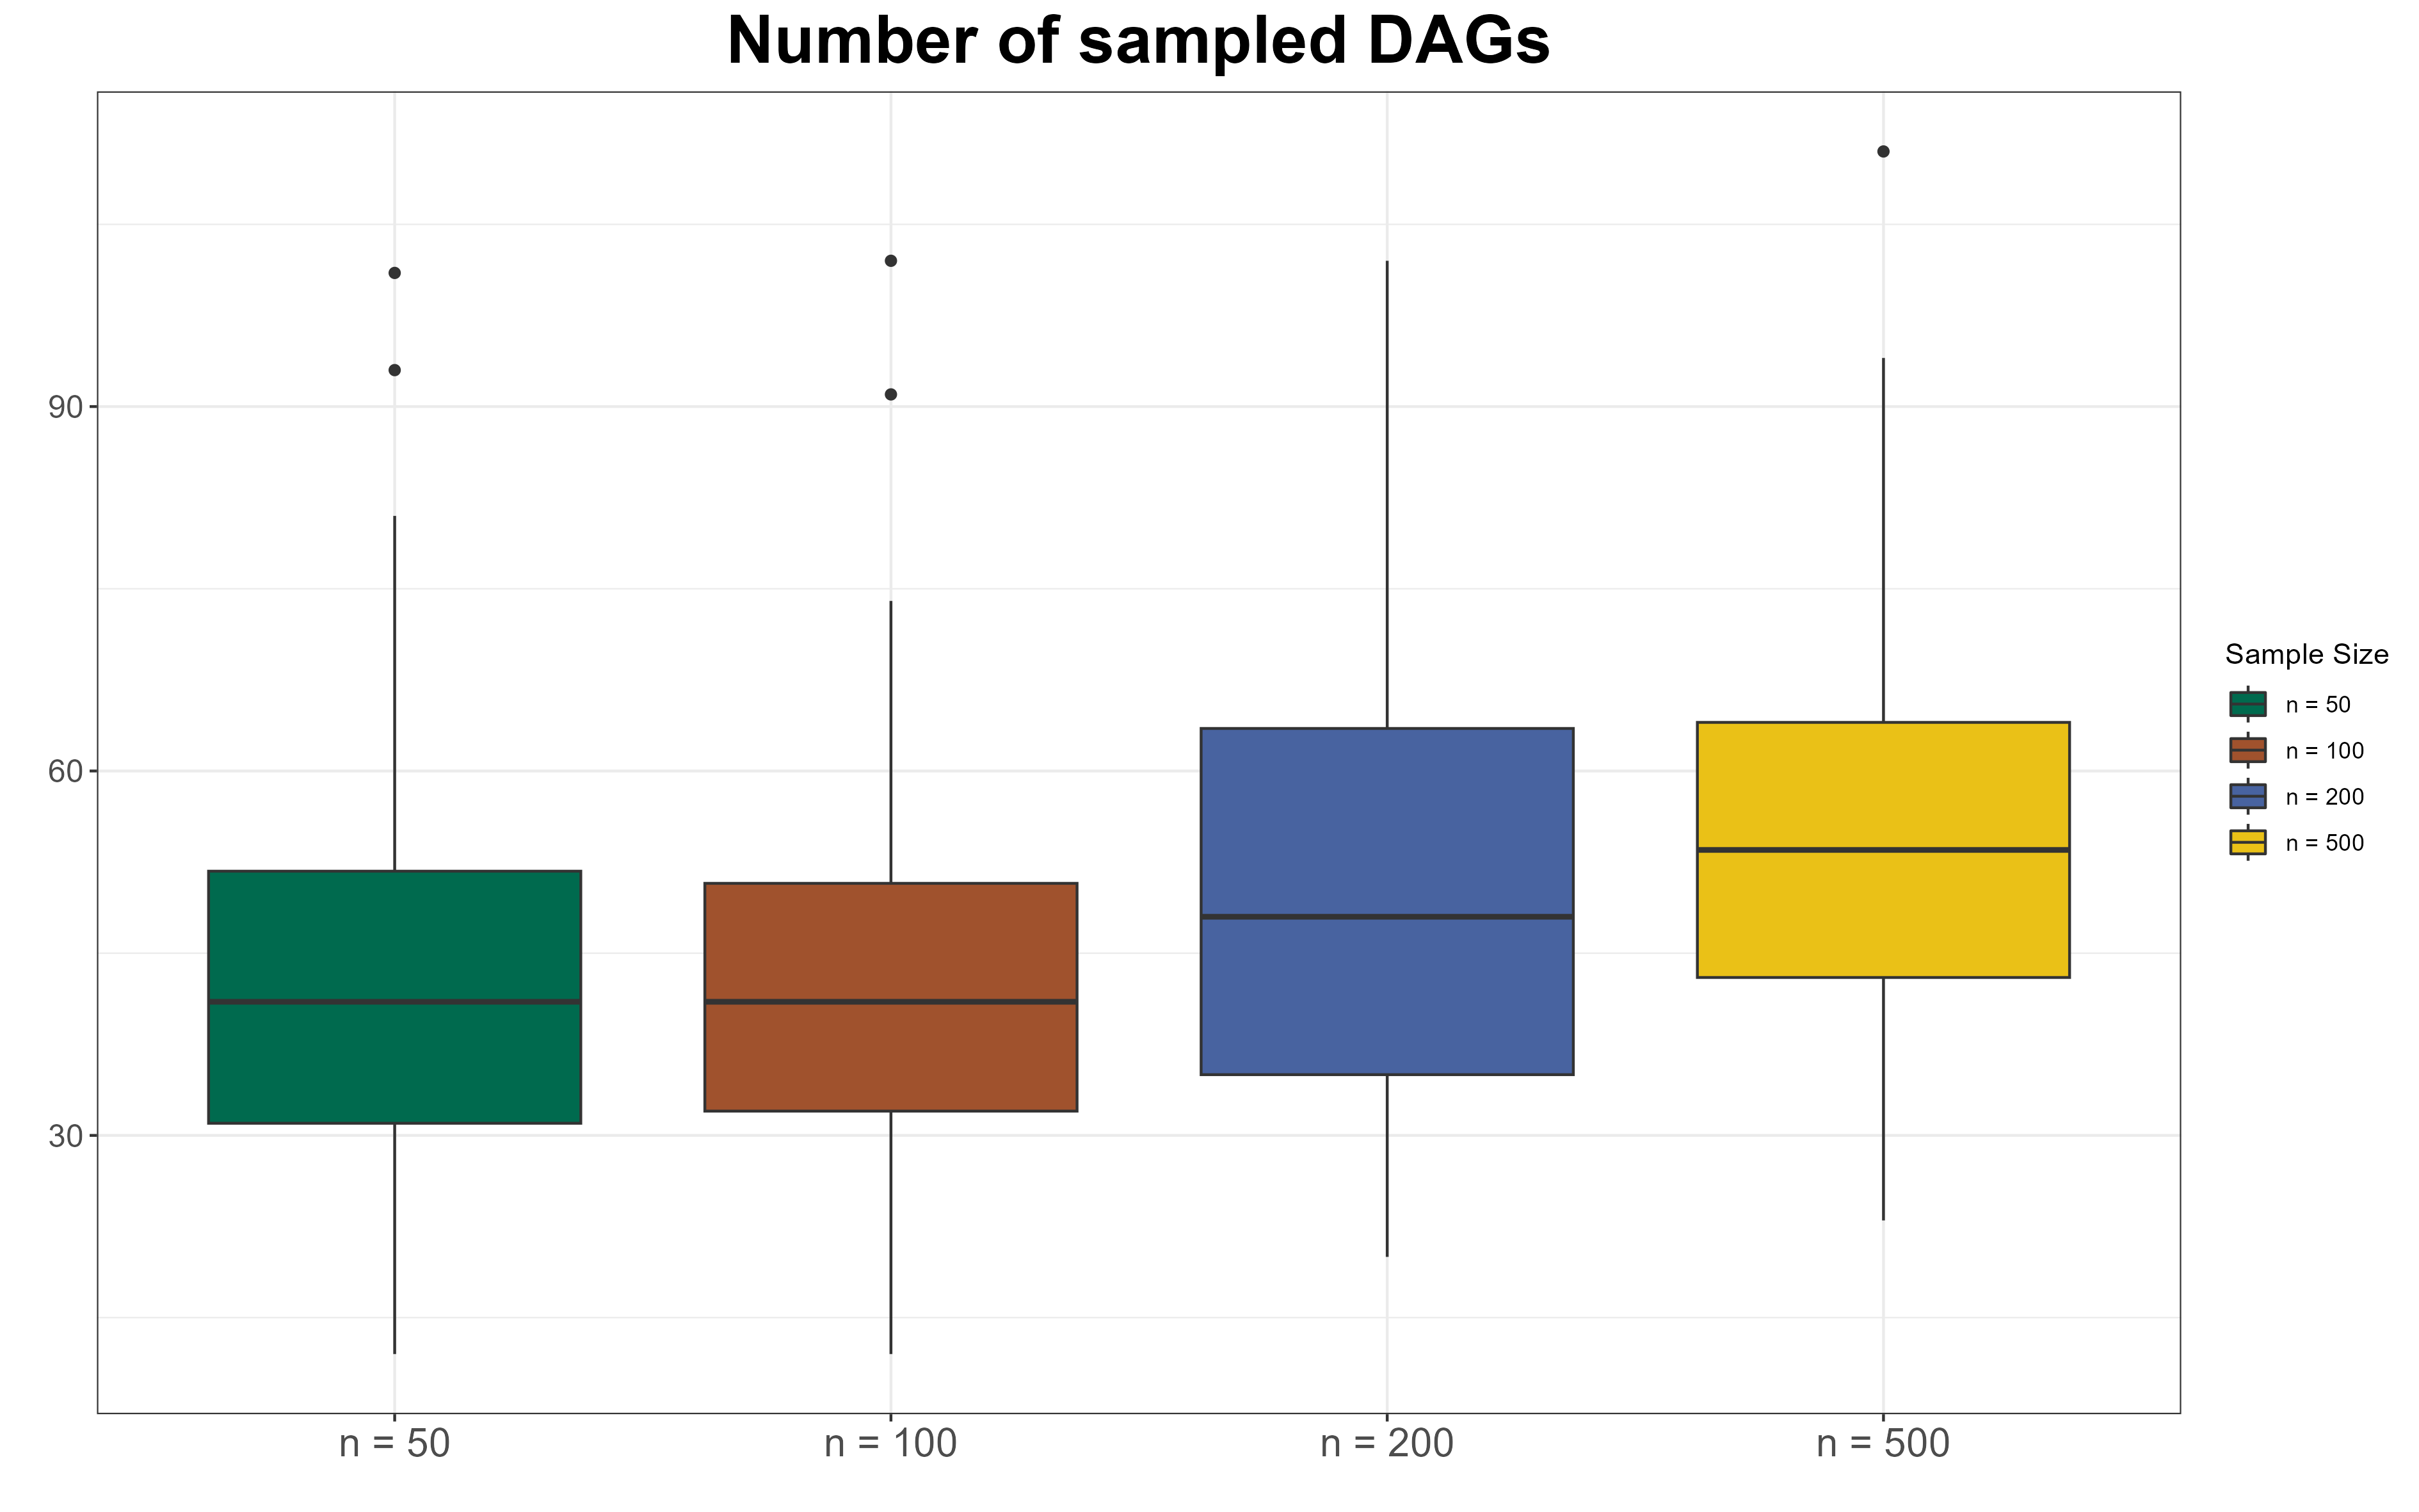
\includegraphics[width=0.5\textwidth]{Figures/Overall_comparison/Boxplot_n_dags.png}
	\caption{Number of unique DAGs explored by the Birth-Death model during the simulation.}
	\label{fig:n-dags}
\end{figure}

In $\textit{Table}$ \ref{table:edge-probs} the color blocks represent the results from the four algorithms, arranged in order of increasing sample size. A general trend can be observed: as the sample size increases, the posterior probabilities also increase, indicating stronger evidence for the existence of dependencies between variables. Interestingly, however, the edge connecting node 7 and node 3 is consistently overlooked by all the algorithms, failing to register any significant posterior probability.

This could suggest that the edge is effectively independent of the rest of the network, meaning its presence or absence does not significantly impact the overall DAG structure. In such cases, the algorithms, which rely on evaluating the contribution of each edge to the model's likelihood and prior, might deem this edge as non-essential. This could explain why the algorithms consistently assign it a low probability of inclusion.


\begin{table}[!ht]
	\raggedleft
	\footnotesize
	\begin{tabular}{|l|l|l|l|l|l|l|}
		\arrayrulecolor{black}
		\hline
		\textbf{From 2 to 1} & \textbf{From 3 to 1} & \textbf{From 7 to 2} & \textbf{From 8 to 2} & \textbf{From 7 to 3} & \textbf{From 5 to 4} & \textbf{From 6 to 4} \\ \hline
		\rowcolor{red!10} 0.5164 (0.0171) & 0.0275 (0.0067) & 0.037 (0.0072) & 0.0387 (0.006) & 0.0101 (0.0035) & 0.9769 (0.0641) & 0.9773 (0.0629) \\ \hline
		\rowcolor{red!10}  0.5595 (0.0295) & 0.3775 (0.0236) & 0.0391 (0.0085) & 0.0918 (0.0113) & 7e-04 (7e-04) & 0.6812 (0.3909) & 0.6815 (0.3906) \\ \hline
		\rowcolor{red!10} 1 (0) & 0.9999 (2e-04) & 0.4904 (0.0097) & 0.4184 (0.016) & 1e-04 (1e-04) & 0.45 (0.5016) & 0.4498 (0.5016) \\ \hline
		\rowcolor{red!10} 1 (0) & 1 (0) & 0.7891 (0.0189) & 0.7938 (0.0204) & 1e-04 (3e-04) & 0.6975 (0.3859) & 0.6974 (0.3857) \\ \hline
		\rowcolor{blue!7} 0.4951 (0.0126) & 0.011 (0.0019) & 0.0176 (0.0019) & 0.0151 (0.003) & 0.0034 (0.001) & 0.981 (0.0489) & 0.9814 (0.049) \\ \hline
		\rowcolor{blue!7} 0.494 (0.1059) & 0.3586 (0.1068) & 0.0088 (0.0018) & 0.0258 (0.0034) & 2e-04 (2e-04) & 0.4132 (0.4984) & 0.4133 (0.4983) \\ \hline
		\rowcolor{blue!7} 0.9896 (0.0222) & 0.9897 (0.022) & 0.4791 (0.0135) & 0.3629 (0.0282) & 0 (0) & 0.5333 (0.5164) & 0.5334 (0.5163) \\ \hline
		\rowcolor{blue!7} 1 (0) & 1 (0) & 0.7903 (0.0088) & 0.7902 (0.0109) & 2e-04 (2e-04) & 0.6584 (0.4411) & 0.6587 (0.4409) \\ \hline
		\rowcolor{cyan!10} 0.4951 (0.0126) & 0.011 (0.0019) & 0.0176 (0.0019) & 0.0151 (0.003) & 0.0034 (0.001) & 0.981 (0.0489) & 0.9814 (0.049) \\ \hline
		\rowcolor{cyan!10} 0.5043 (0.0664) & 0.3646 (0.0594) & 0.0113 (0.0028) & 0.0334 (0.0045) & 3e-04 (3e-04) & 0.7834 (0.4104) & 0.7835 (0.4103) \\ \hline
		\rowcolor{cyan!10} 0.9999 (4e-04) & 0.9999 (5e-04) & 0.4806 (0.0148) & 0.3843 (0.0156) & 0 (1e-04) & 0.6 (0.5071) & 0.6 (0.5071) \\ \hline
		\rowcolor{cyan!10} 1 (0) & 0.9999 (2e-04) & 0.7891 (0.01) & 0.7893 (0.0095) & 2e-04 (3e-04) & 0.6053 (0.4767) & 0.6054 (0.4765) \\ \hline
		\rowcolor{green!8} 0.4092 (0.2248) & 0.0186 (0.0348) & 0.0323 (0.0491) & 0.0227 (0.039) & 0.0045 (0.0076) & 0.8958 (0.1725) & 0.7835 (0.3196) \\ \hline
		\rowcolor{green!8}0.9136 (0.2671) & 0.8492 (0.2859) & 0.0558 (0.1023) & 0.5445 (0.3728) & 0.001 (0.0019) & 0.8999 (0.1672) & 0.7515 (0.3285) \\ \hline
		\rowcolor{green!8} 0.9661 (0.1684) & 0.656 (0.3791) & 0.5237 (0.408) & 0.4951 (0.453) & 1e-04 (3e-04) & 0.9868 (0.0933) & 0.7243 (0.3769) \\ \hline
		\rowcolor{green!8} 0.8594 (0.3503) & 0.6779 (0.4144) & 0.8203 (0.2973) & 0.6812 (0.393) & 0 (0) & 1 (0) & 0.7302 (0.3552) \\ \hline
	\end{tabular}
	\caption{Edge probabilities with corresponding standard errors (in parentheses) across algorithms and numerosity, estimated as the average across replicates. Only edges present in the true DAG are shown in the table.}
	\label{table:edge-probs}
\end{table}

\subsection{Performance metrics}

The evaluation of the algorithm’s performance in selecting the true DAG structure involves several key metrics. True Positives occur when the algorithm correctly identifies an edge that exists in the true DAG. Conversely, True Negatives represent cases where the algorithm correctly identifies the absence of an edge, indicating its effectiveness in avoiding overfitting by excluding non-existent dependencies. On the other hand, False Positives are instances where the algorithm incorrectly identifies an edge that does not exist in the true DAG. Meanwhile, False Negatives occur when the algorithm fails to detect an edge that is present in the true DAG, leading to an incomplete or incorrect understanding of the network structure.

Moreover, to assess the algorithm’s detection capabilities, Sensitivity is used, which measures the proportion of actual edges that are correctly identified, calculated as $\frac{\text{TP}}{\text{TP} + \text{FN}}$. High sensitivity indicates that the algorithm effectively captures true edges, which is crucial in minimizing the omission of important dependencies. Specificity, calculated as $\frac{\text{TN}}{\text{TN} + \text{FP}}$, evaluates the proportion of non-existent edges that are correctly identified, thereby ensuring the algorithm avoids unnecessary complexity by rejecting spurious edges.

Precision is another important metric, quantifying the proportion of predicted edges that are actual positives, given by $\frac{\text{TP}}{\text{TP} + \text{FP}}$. High precision reflects a low rate of false positives, ensuring that detected edges are likely to be true. Balancing Precision and Sensitivity, the F1 Score provides a single metric that captures the trade-off between these two aspects, defined as $2 \times \frac{\text{Precision} \times \text{Sensitivity}}{\text{Precision} + \text{Sensitivity}}$.

Finally, the Matthews Correlation Coefficient (MCC) offers a comprehensive evaluation, calculated as $\frac{\text{TP} \times \text{TN} - \text{FP} \times \text{FN}}{\sqrt{(\text{TP} + \text{FP})(\text{TP} + \text{FN})(\text{TN} + \text{FP})(\text{TN} + \text{FN})}}$. The MCC is particularly valuable in scenarios with class imbalances, providing a balanced measure of the algorithm’s overall performance in accurately reconstructing the network.
This metric is the only binary classification rate that generates a high score only if the binary predictor was able to correctly predict the majority of positive data instances and the majority of negative data instances. It ranges in the interval $[ -1, +1]$, with extreme values, 1 and $+ 1$, reached in case of perfect misclassification and perfect classification, respectively, while MCC = 0 is the expected value for the coin tossing classifier (\citet{chicco2020advantages}).    

$\textit{Table} \  \ref{table:metrics-first}$ summarizes the performance of the Metropolis, Adaptive Metropolis, and BDMCMC algorithms across different sample sizes, revealing distinct trends in how these algorithms handle edge detection in the true DAG. For the Metropolis algorithm (first four rows), there is a clear increase in True Positives (TP) as the sample size grows from 50 to 500, with TP values rising from 2.87 to 5.33. This indicates that the algorithm becomes significantly better at identifying true edges in the DAG with more data. The corresponding decrease in False Negatives (FN) from 4.13 to 1.67 further supports this. However, the True Negative (TN) and False Positive (FP) counts remain relatively constant, suggesting that the Metropolis algorithm’s ability to avoid false detections does not change much with larger datasets.

The Adaptive Metropolis algorithm (rows 5-12) follows a similar pattern, with increasing sample sizes leading to higher TP rates and lower FN rates, particularly noticeable as the sample size reaches 500. However, the Adaptive algorithm displays slightly more variability in FP rates at smaller sample sizes, indicating that it may be more sensitive to false positives initially. As the sample size increases, the algorithm stabilizes, showing consistent performance with fewer false positives and a high TN rate, indicating that it effectively balances sensitivity and specificity with more data.

The BDMCMC algorithm (last four rows) exhibits a more dynamic response to increasing sample sizes. Initially, with a smaller sample size, BDMCMC has lower TP and higher FN rates, indicating a conservative approach that prioritizes avoiding false positives at the cost of missing some true edges. As the sample size grows to 500, the TP rate improves significantly to 4.74, while the FN rate decreases to 2.26, suggesting that BDMCMC becomes more adept at detecting true edges with sufficient data. However, this improvement in sensitivity comes with a slight increase in FP rates, indicating a trade-off where BDMCMC becomes more prone to detecting edges that may not exist. This behavior suggests that BDMCMC, while highly effective at larger sample sizes, may require careful tuning to balance its sensitivity and specificity, especially when false positives need to be minimized.

\begin{table}[!h]
	\centering
	\begin{tabular}{|l|l|l|l|l|}
		\hline
		\textbf{} & \textbf{True Positive} & \textbf{True Negative} & \textbf{False Positive} & \textbf{False Negative} \\ \hline
		\rowcolor{red!10} \textbf{1} & 2.867 (0.352) & 56.867 (0.352) & 0.133 (0.352) & 4.133 (0.352) \\ \hline
		\rowcolor{red!10} \textbf{2} & 2.333 (0.976) & 56.333 (0.976) & 0.667 (0.976) & 4.667 (0.976) \\ \hline
		\rowcolor{red!10} \textbf{3} & 3.133 (1.06) & 55.6 (1.183) & 1.4 (1.183) & 3.867 (1.06) \\ \hline
		\rowcolor{red!10} \textbf{4} & 5.333 (0.976) & 56.333 (0.976) & 0.667 (0.976) & 1.667 (0.976) \\ \hline
		\rowcolor{blue!7} \textbf{5} & 2.4 (0.507) & 56.4 (0.507) & 0.6 (0.507) & 4.6 (0.507) \\ \hline
		\rowcolor{blue!7} \textbf{6} & 1.333 (1.345) & 55.133 (1.187) & 1.867 (1.187) & 5.667 (1.345) \\ \hline
		\rowcolor{blue!7} \textbf{7} & 3.067 (1.033) & 55.6 (1.056) & 1.4 (1.056) & 3.933 (1.033) \\ \hline
		\rowcolor{blue!7} \textbf{8} & 5.333 (0.976) & 56.333 (0.976) & 0.667 (0.976) & 1.667 (0.976) \\ \hline
		\rowcolor{cyan!10} \textbf{9} & 2.4 (0.507) & 56.4 (0.507) & 0.6 (0.507) & 4.6 (0.507) \\ \hline
		\rowcolor{cyan!10} \textbf{10} & 2.133 (0.743) & 56.133 (0.743) & 0.867 (0.743) & 4.867 (0.743) \\ \hline
		\rowcolor{cyan!10} \textbf{11} & 3.333 (0.9) & 55.733 (1.033) & 1.267 (1.033) & 3.667 (0.9) \\ \hline
		\rowcolor{cyan!10} \textbf{12} & 5.2 (1.014) & 56.2 (1.014) & 0.8 (1.014) & 1.8 (1.014) \\ \hline
		\rowcolor{green!8} \textbf{13} & 1.36 (0.985) & 55 (1.457) & 2 (1.457) & 5.64 (0.985) \\ \hline
		\rowcolor{green!8} \textbf{14} & 3.84 (1.201) & 55.56 (1.473) & 1.44 (1.473) & 3.16 (1.201) \\ \hline
		\rowcolor{green!8} \textbf{15} & 3.98 (1.059) & 54.12 (1.955) & 2.88 (1.955) & 3.02 (1.059) \\ \hline
		\rowcolor{green!8} \textbf{16} & 4.74 (0.965) & 54.7 (1.693) & 2.3 (1.693) & 2.26 (0.965) \\ \hline
	\end{tabular}
	\caption{True Positive, True Negative, False Positive, and False Negative rates with corresponding standard errors (in parentheses) across algorithms and numerosity, estimated as the average across replicates. Red rows show plain Metropolis results, purple and blue indicate adaptive Metropolis (C = 0.5 and C = 0.7) and green represents BDMCMC.}
	\label{table:metrics-first}
\end{table}

Higher F1 Scores ($\textit{Table}$ \ref{table:metrics-second}), particularly in the later rows as the sample size increases, indicate that the algorithms become more proficient at correctly identifying the edges while minimizing errors. Notably, the BDMCMC algorithm shows substantial improvements in its F1 Score, reflecting its ability to correctly identify more edges while minimizing false detections.

\begin{table}[!h]
	\centering
	\begin{tabular}{|l|l|l|l|l|l|}
		\hline
		\textbf{} & \textbf{Sensitivity} & \textbf{Specificity} & \textbf{Precision} & \textbf{F1 Score} & \textbf{MCC} \\ \hline
		\rowcolor{red!10} \textbf{1} & 0.41 (0.05) & 0.998 (0.006) & 0.956 (0.117) & 0.573 (0.07) & 0.601 (0.083) \\ \hline
		\rowcolor{red!10} \textbf{2} & 0.333 (0.139) & 0.988 (0.017) & 0.778 (0.325) & 0.467 (0.195) & 0.475 (0.231) \\ \hline
		\rowcolor{red!10} \textbf{3} & 0.448 (0.151) & 0.975 (0.021) & 0.7 (0.251) & 0.544 (0.186) & 0.518 (0.211) \\ \hline
		\rowcolor{red!10} \textbf{4} & 0.762 (0.139) & 0.988 (0.017) & 0.889 (0.163) & 0.821 (0.15) & 0.803 (0.168) \\ \hline
		\rowcolor{blue!7} \textbf{5} & 0.343 (0.072) & 0.989 (0.009) & 0.8 (0.169) & 0.48 (0.101) & 0.491 (0.12) \\ \hline
		\rowcolor{blue!7} \textbf{6} & 0.19 (0.192) & 0.967 (0.021) & 0.4 (0.397) & 0.257 (0.257) & 0.22 (0.296) \\ \hline
		\rowcolor{blue!7} \textbf{7} & 0.438 (0.148) & 0.975 (0.019) & 0.691 (0.235) & 0.534 (0.176) & 0.507 (0.199) \\ \hline
		\rowcolor{blue!7} \textbf{8} & 0.762 (0.139) & 0.988 (0.017) & 0.889 (0.163) & 0.821 (0.15) & 0.803 (0.168) \\ \hline
		\rowcolor{cyan!10} \textbf{9} & 0.343 (0.072) & 0.989 (0.009) & 0.8 (0.169) & 0.48 (0.101) & 0.491 (0.12) \\ \hline
		\rowcolor{cyan!10} \textbf{10} & 0.305 (0.106) & 0.985 (0.013) & 0.711 (0.248) & 0.427 (0.149) & 0.428 (0.176) \\ \hline
		\rowcolor{cyan!10} \textbf{11} & 0.476 (0.129) & 0.978 (0.018) & 0.733 (0.219) & 0.576 (0.159) & 0.551 (0.181) \\ \hline
		\rowcolor{cyan!10} \textbf{12} & 0.743 (0.145) & 0.986 (0.018) & 0.867 (0.169) & 0.8 (0.156) & 0.78 (0.174) \\ \hline
		\rowcolor{green!8} \textbf{13} & 0.194 (0.141) & 0.965 (0.026) & 0.45 (0.33) & 0.271 (0.197) & 0.239 (0.24) \\ \hline
		\rowcolor{green!8} \textbf{14} & 0.549 (0.172) & 0.975 (0.026) & 0.743 (0.266) & 0.629 (0.207) & 0.6 (0.235) \\ \hline
		\rowcolor{green!8} \textbf{15} & 0.569 (0.151) & 0.949 (0.034) & 0.611 (0.235) & 0.586 (0.189) & 0.537 (0.217) \\ \hline
		\rowcolor{green!8} \textbf{16} & 0.677 (0.138) & 0.96 (0.03) & 0.695 (0.209) & 0.684 (0.171) & 0.645 (0.195) \\ \hline
	\end{tabular}
	\caption{Sensitivity, Specificity, Precision, F1 Score, MCC rates with corresponding standard errors (in parentheses) across algorithms and numerosity, estimated as the average across replicates. Red rows show plain Metropolis results, purple and blue indicate adaptive Metropolis (C = 0.5 and C = 0.7) and green represents BDMCMC.}
	\label{table:metrics-second}
\end{table}

\begin{figure}[h] 
	\centering
	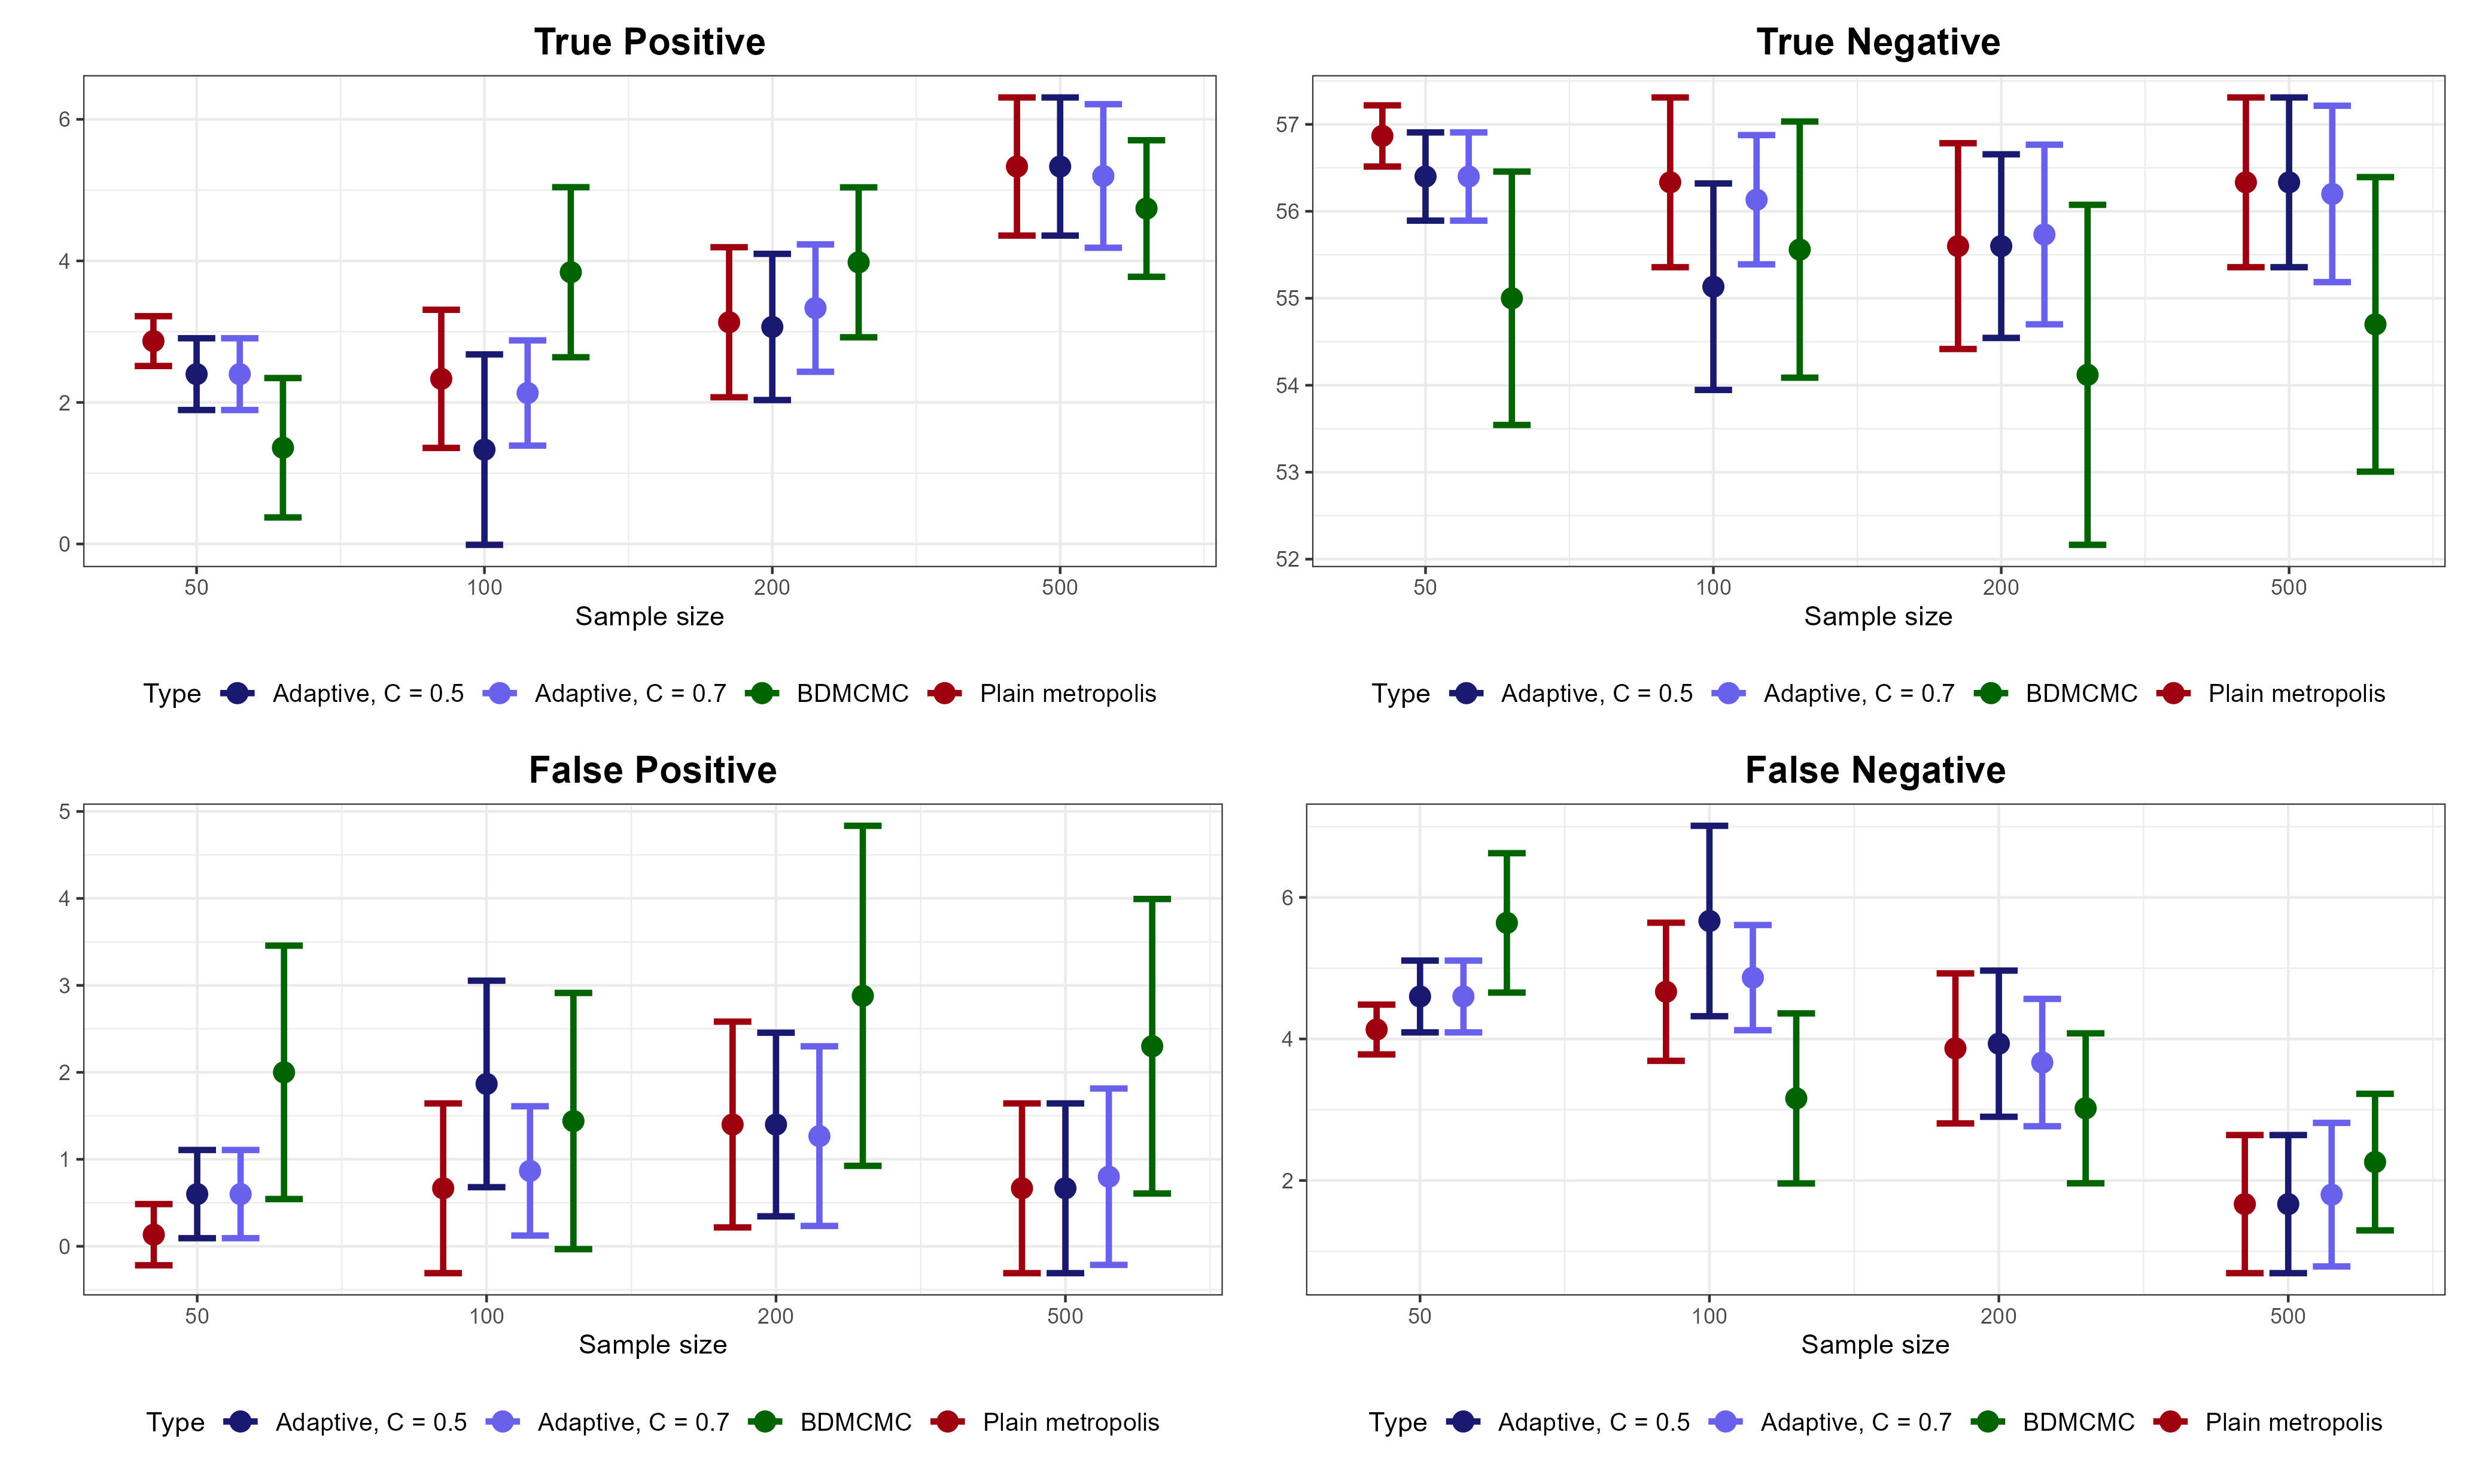
\includegraphics[width=1.0\textwidth]{Figures/Overall_comparison/metric_plots1.png}
	\caption{True Positive, True Negative, False Positive, and False Negative rates graphically represented with standard errors as vertical error bars. }
	\label{fig:metric-plots1}
\end{figure}

\begin{figure}[h] 
	\centering
	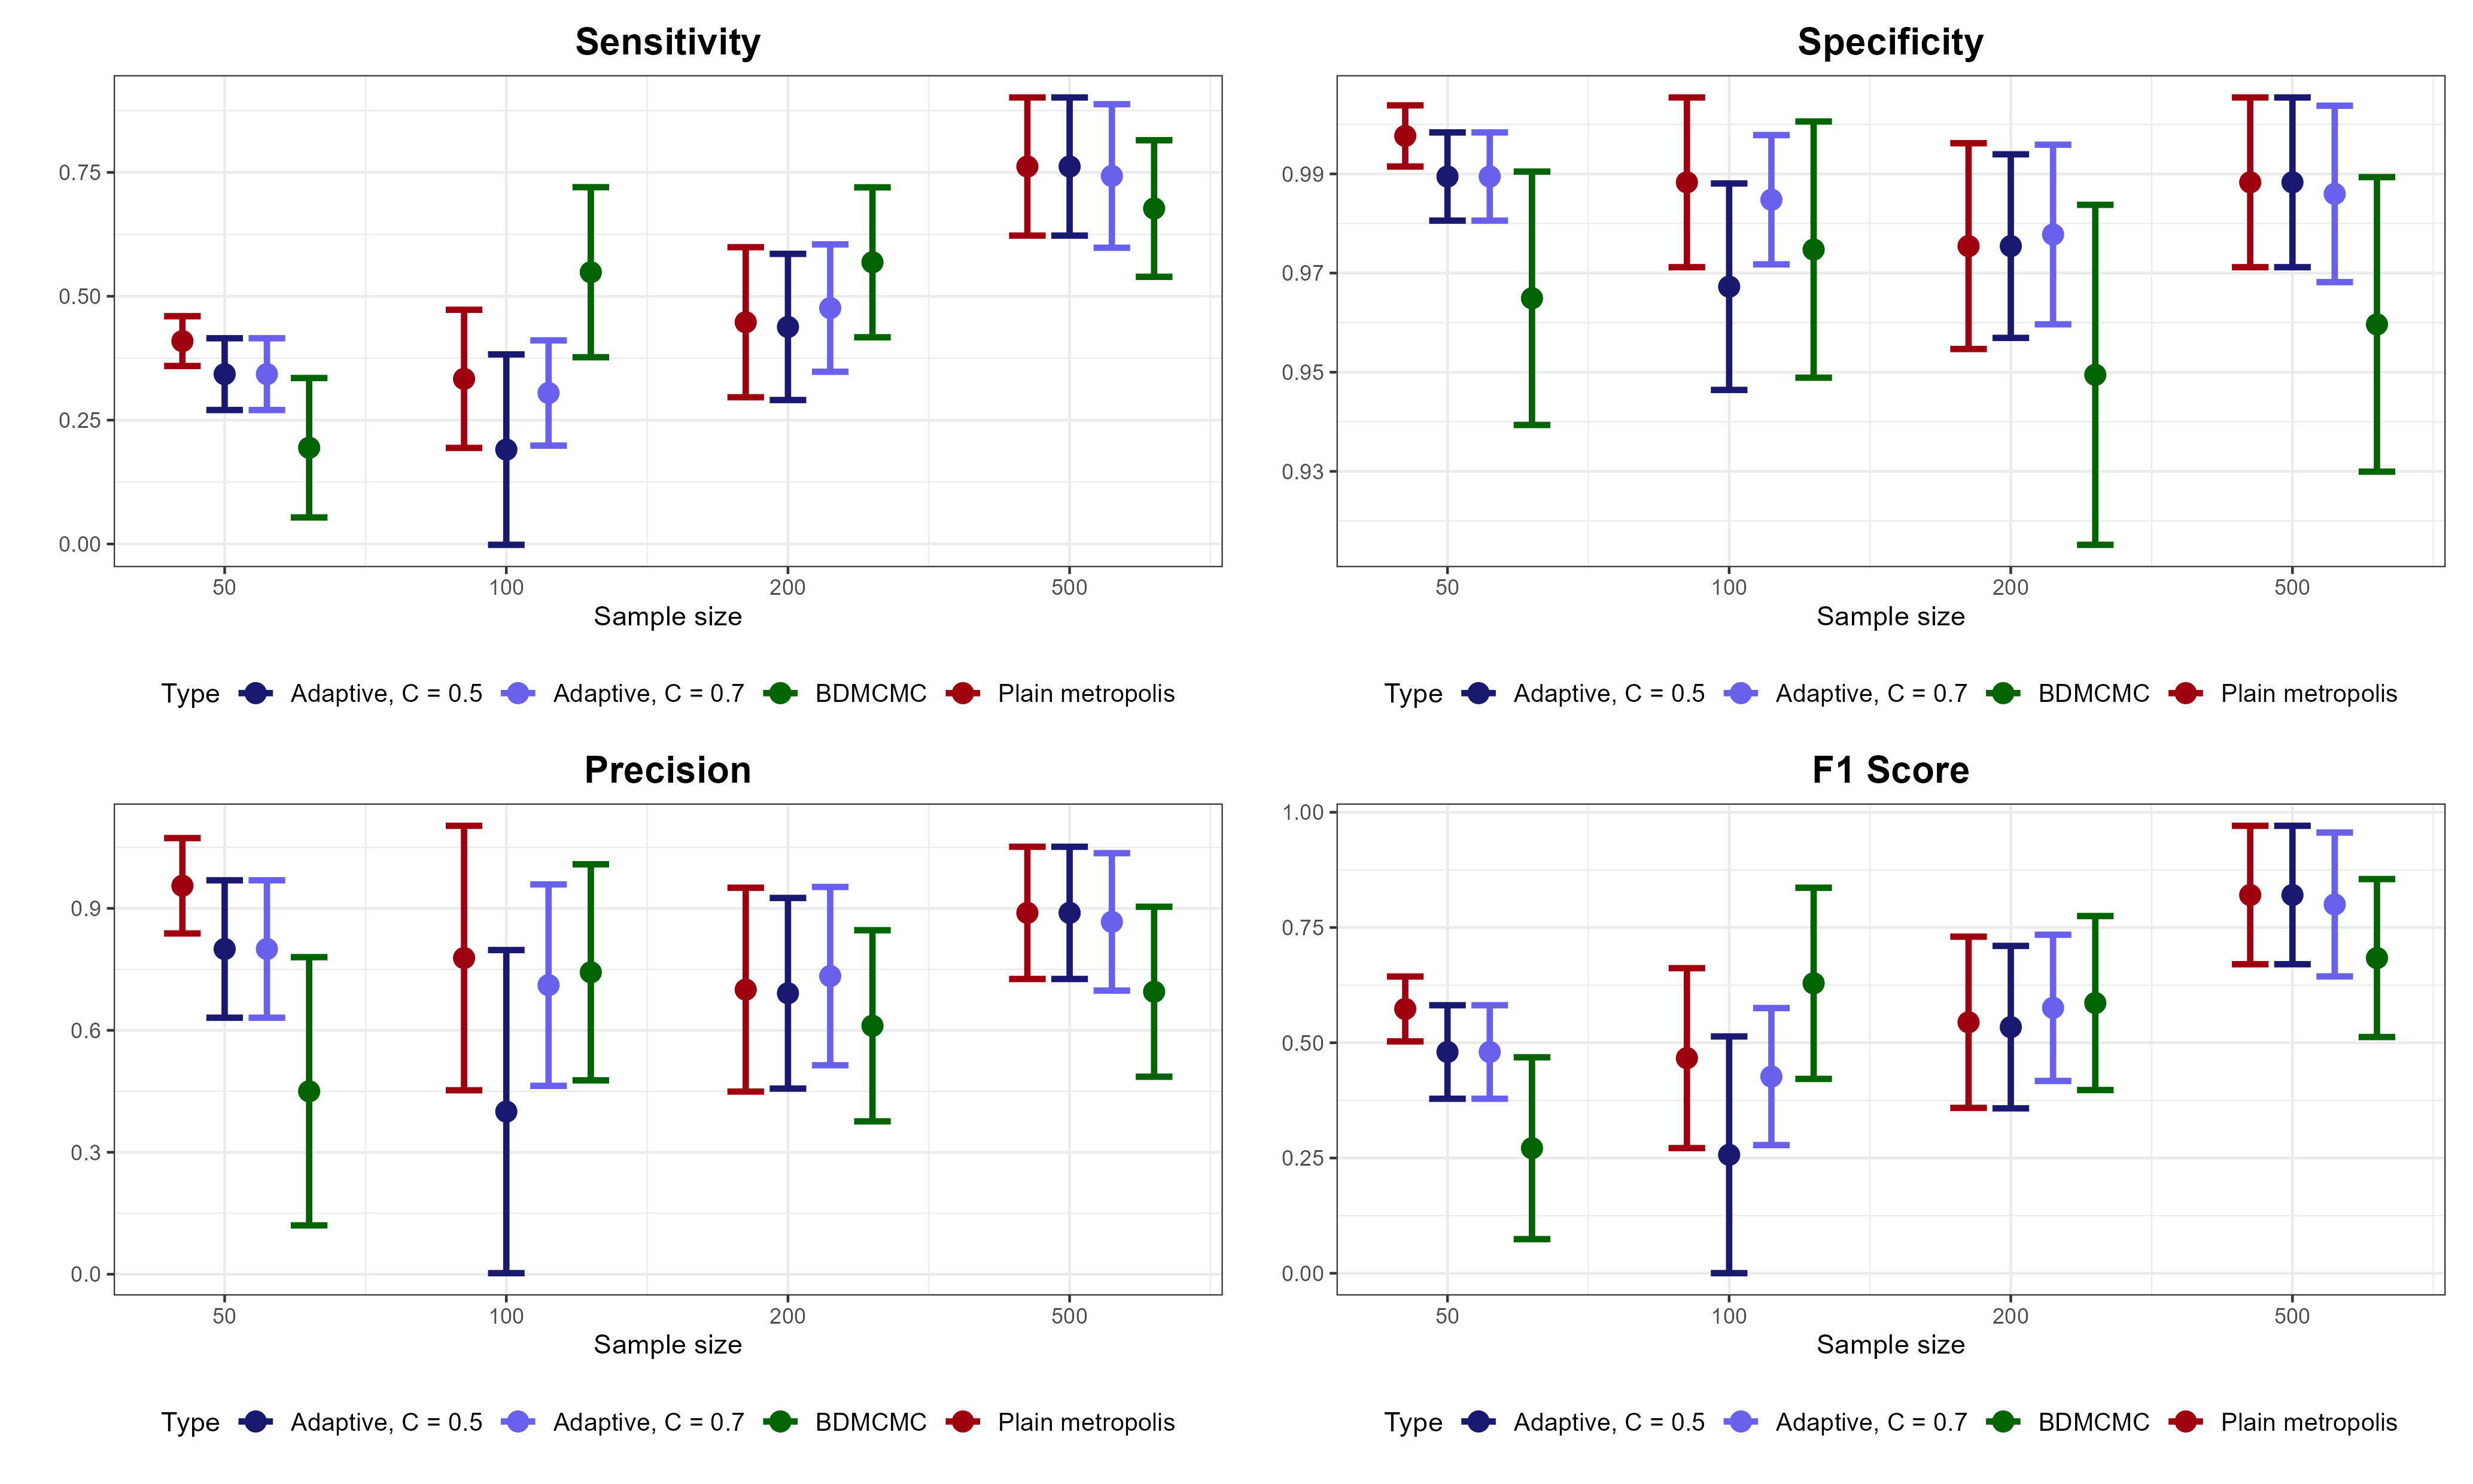
\includegraphics[width=1.0\textwidth]{Figures/Overall_comparison/metric_plots2.png}
	\caption{Sensitivity, Specificity, Precision, F1 Score rates graphically represented with standard errors as vertical error bars.}
	\label{fig:metric-plots2}
\end{figure}

\begin{figure}[h] 
	\centering
	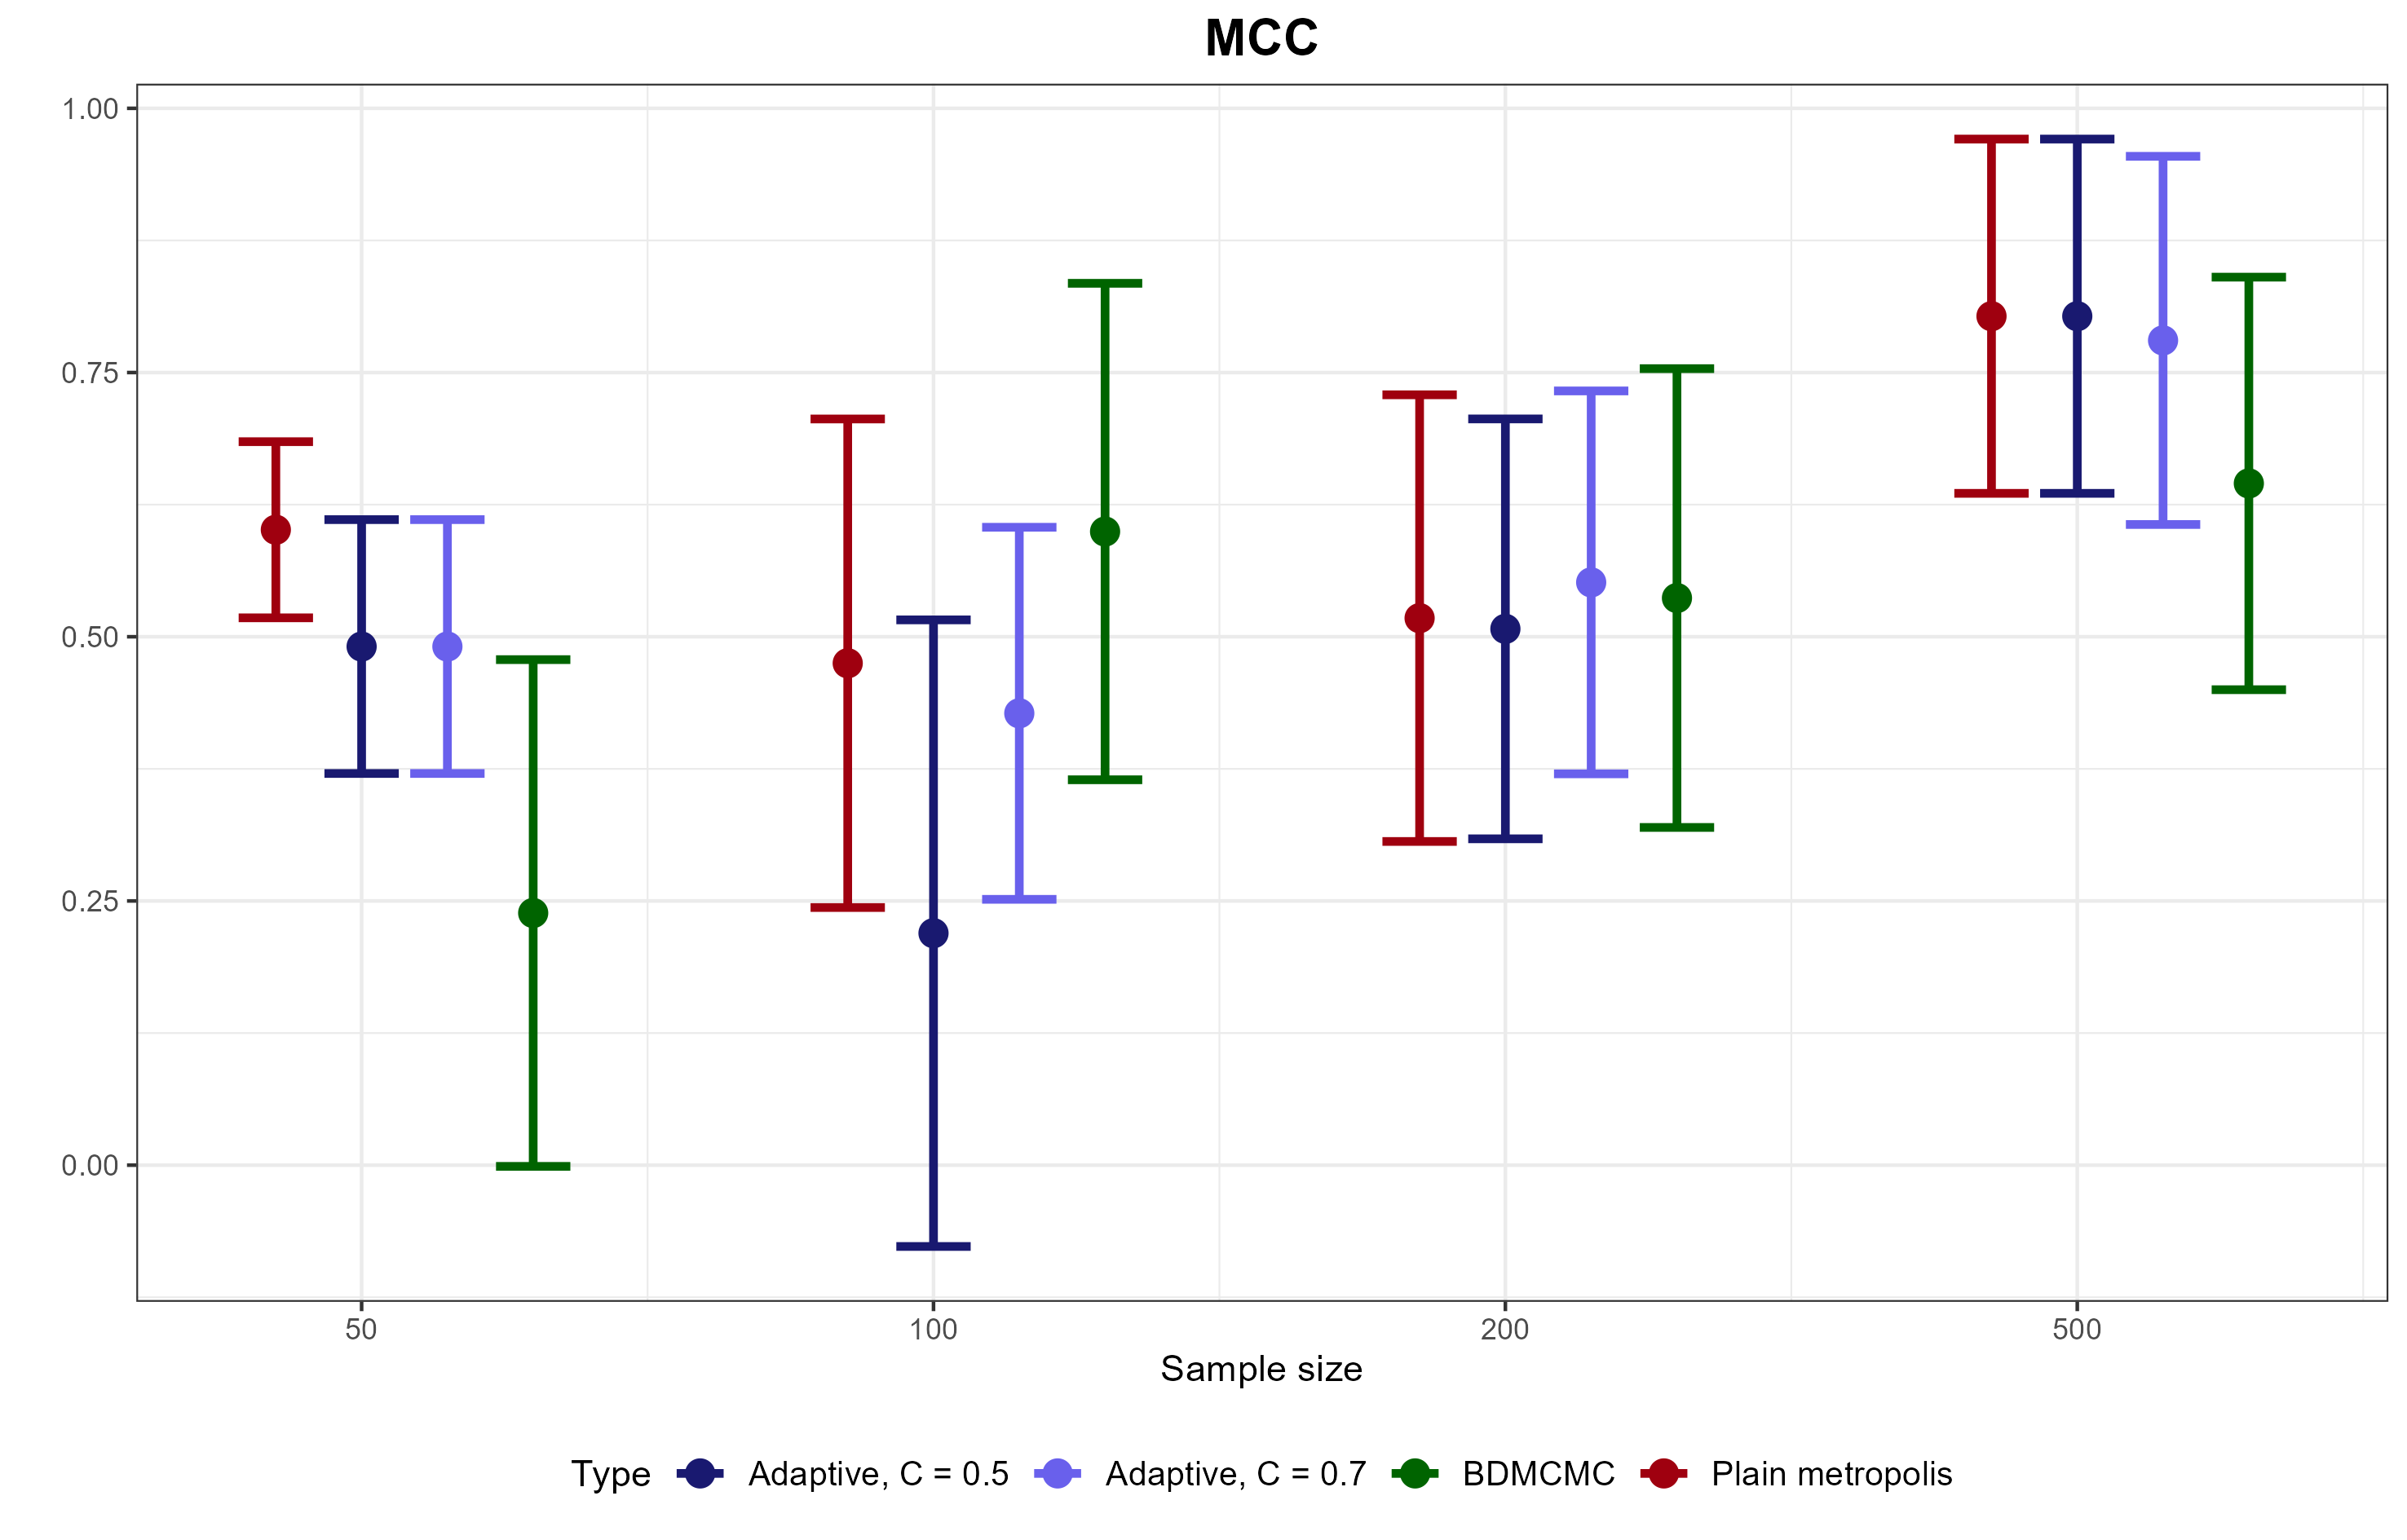
\includegraphics[width=0.5\textwidth]{Figures/Overall_comparison/MCC.png}
	\caption{MCC rate graphically represented with standard errors as vertical error bars.}
	\label{fig:metric-mmc}
\end{figure}

Same results are also provided in graphical form, specifically in \textit{Figures} \ref{fig:metric-plots1}, \ref{fig:metric-plots2} and \ref{fig:metric-mmc}.

\subsubsection{Kullback-Leibler divergence on Sigma estimation}

The Kullback Leibler distance between two probability mass functions $g(x)$ and $h(x)$ is defined as (\citet{cover1999elements}):

$$
D(g || h) = \int^{+\infty}_{-\infty} g(x) In \frac{g(x)}{h(x)} dx
$$

The KLD is always non-negative and equals zero only if the two distributions  being compared are identical, meaning there is no divergence between them.  Beyond simply measuring divergence, KLD can be viewed as a measure of information gain or loss. Specifically, it quantifies the amount of information lost when one distribution is used to approximate another. In practical terms, a higher KLD value indicates greater disparity between the two distributions, implying that the approximation is less accurate and more information is lost.

In this case the measure is computed between the true and estimated Sigma matrix. Computations are carried out as follows: 

$$
\text{KL}(\Sigma_{\text{true}}, \Sigma_{\text{est}}) = \frac{1}{2} \left( \text{tr}\left( \Sigma_{\text{true}}^{-1} \cdot \Sigma_{\text{est}} \right) - p - \log \left( \frac{\det(\Sigma_{\text{est}})}{\det(\Sigma_{\text{true}})} \right) \right)
$$

where $\text{tr}(\cdot)$ denotes the trace of a matrix, $\det(\cdot)$ is the matrix determinant, and $p$ is the dimensionality of the covariance matrix. The first term, $\text{tr}\left( \Sigma_{\text{true}}^{-1} \cdot \Sigma_{\text{est}} \right)$, captures the overall similarity between the estimated and true matrices, while the determinant ratio $\frac{\det(\Sigma_{\text{est}})}{\det(\Sigma_{\text{true}})}$ penalizes differences in the spread of the two distributions. 

The results in \textit{Figure} \ref{fig:kl-overall} indicate that the adaptive algorithm delivers the most stable estimates, highlighting its capacity to refine posterior probabilities through its adaptive nature. As expected, all algorithms show a consistent reduction in divergence from the true $\Sigma$ matrix as the sample size increases.

\textit{Table} \ref{table:Kullback-leibler} shows the Kullback-Leibler (KL) divergence and standard errors for the four MCMC algorithms.
For small sample sizes ($n = 50$), all algorithms show relatively high KL divergence, with BDMCMC performing the worst (0.639), suggesting that limited data hampers accurate edge detection. As sample size increases, KL divergence decreases notably, with BDMCMC achieving the lowest value for $n = 500$ (0.047), demonstrating superior performance in large sample settings.

Standard errors are highest for BDMCMC at smaller $n$, indicating greater variability in its estimates. However, with increasing $n$, its standard error significantly decreases, suggesting improved stability. The adaptive MCMC methods show consistent performance gains over Plain Metropolis, with both $C = 0.5$ and $C = 0.7$ yielding more reliable estimates across all sample sizes.
Overall, BDMCMC is the most effective at capturing the true model for larger $n$, while the adaptive methods are competitive throughout. Plain Metropolis lags behind, especially with smaller samples, showing limited structural learning.

\begin{figure}[!ht]
	\centering
	\resizebox{\textwidth}{4.5cm}{  
		\begin{minipage}{\textwidth}
			\centering
			
			% First figure
			\begin{subfigure}[b]{0.45\textwidth} 
				\centering
				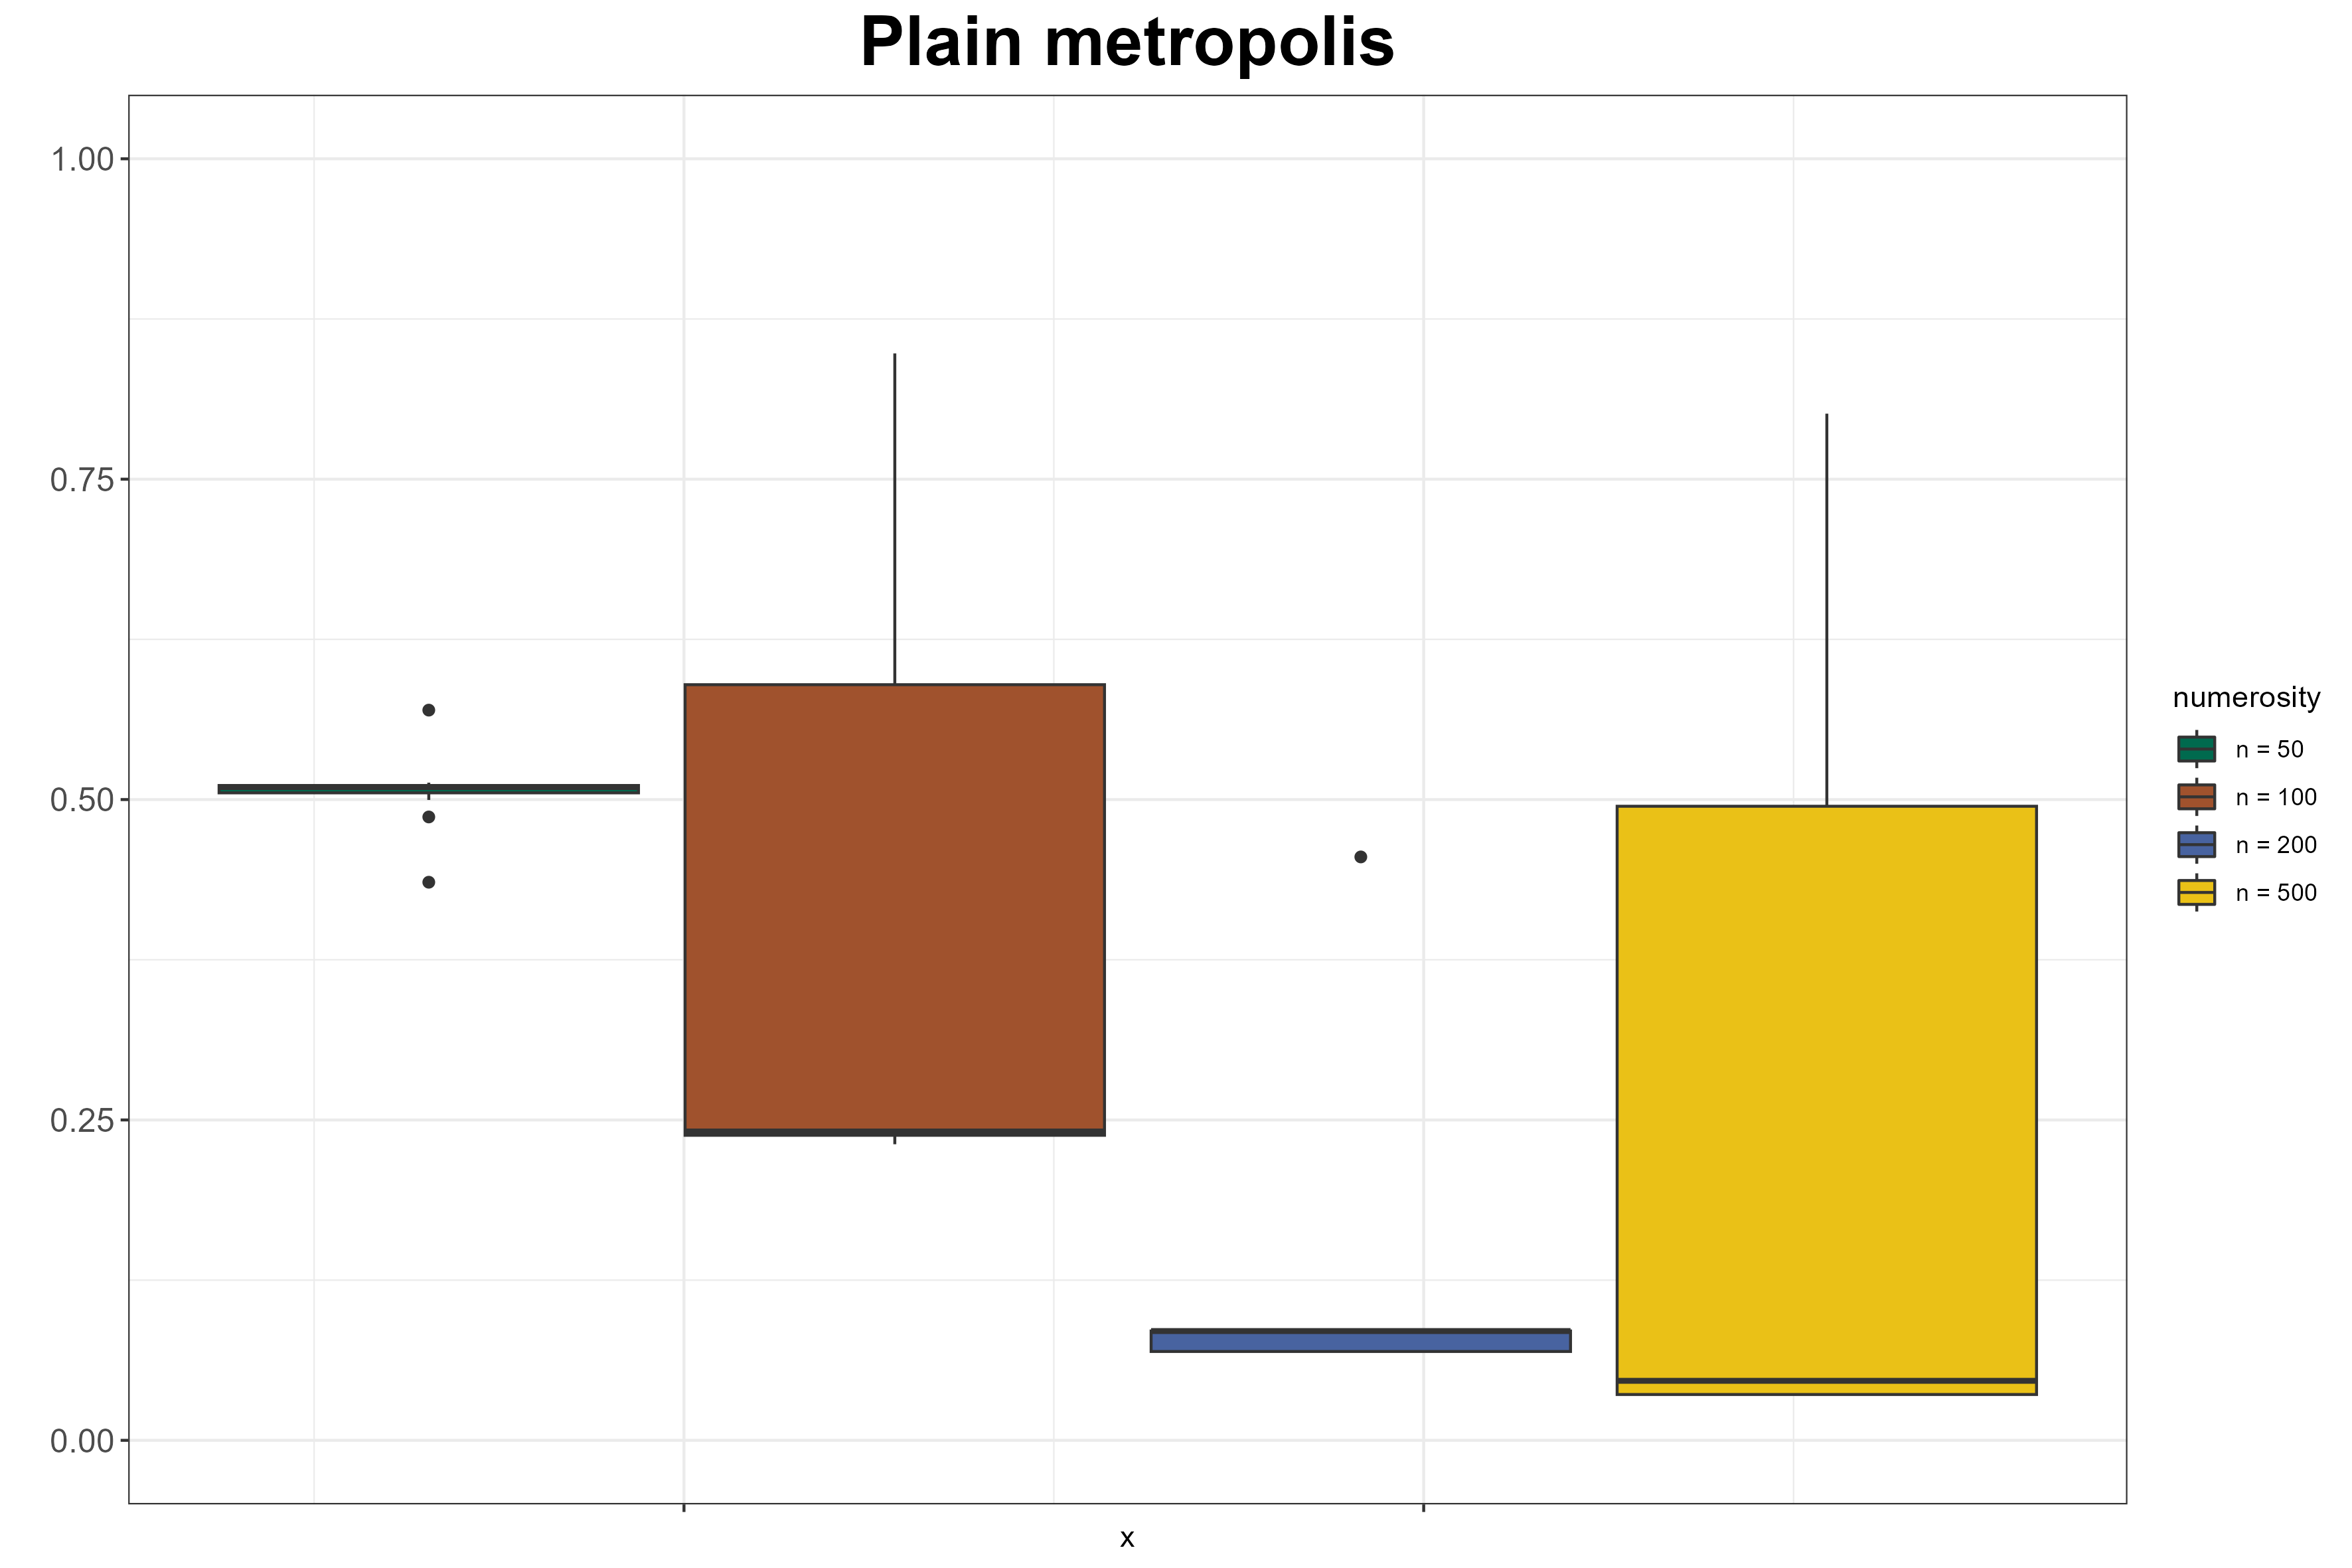
\includegraphics[height=3.5cm]{Figures/Overall_comparison/Boxplot_KL_plain.png}
				%\caption{Sample size 50}
				\label{fig:kl-50}
			\end{subfigure}
			\hspace{0.35cm}  %  horizontal space between figures
			% Second figure
			\begin{subfigure}[b]{0.45\textwidth}   
				\centering
				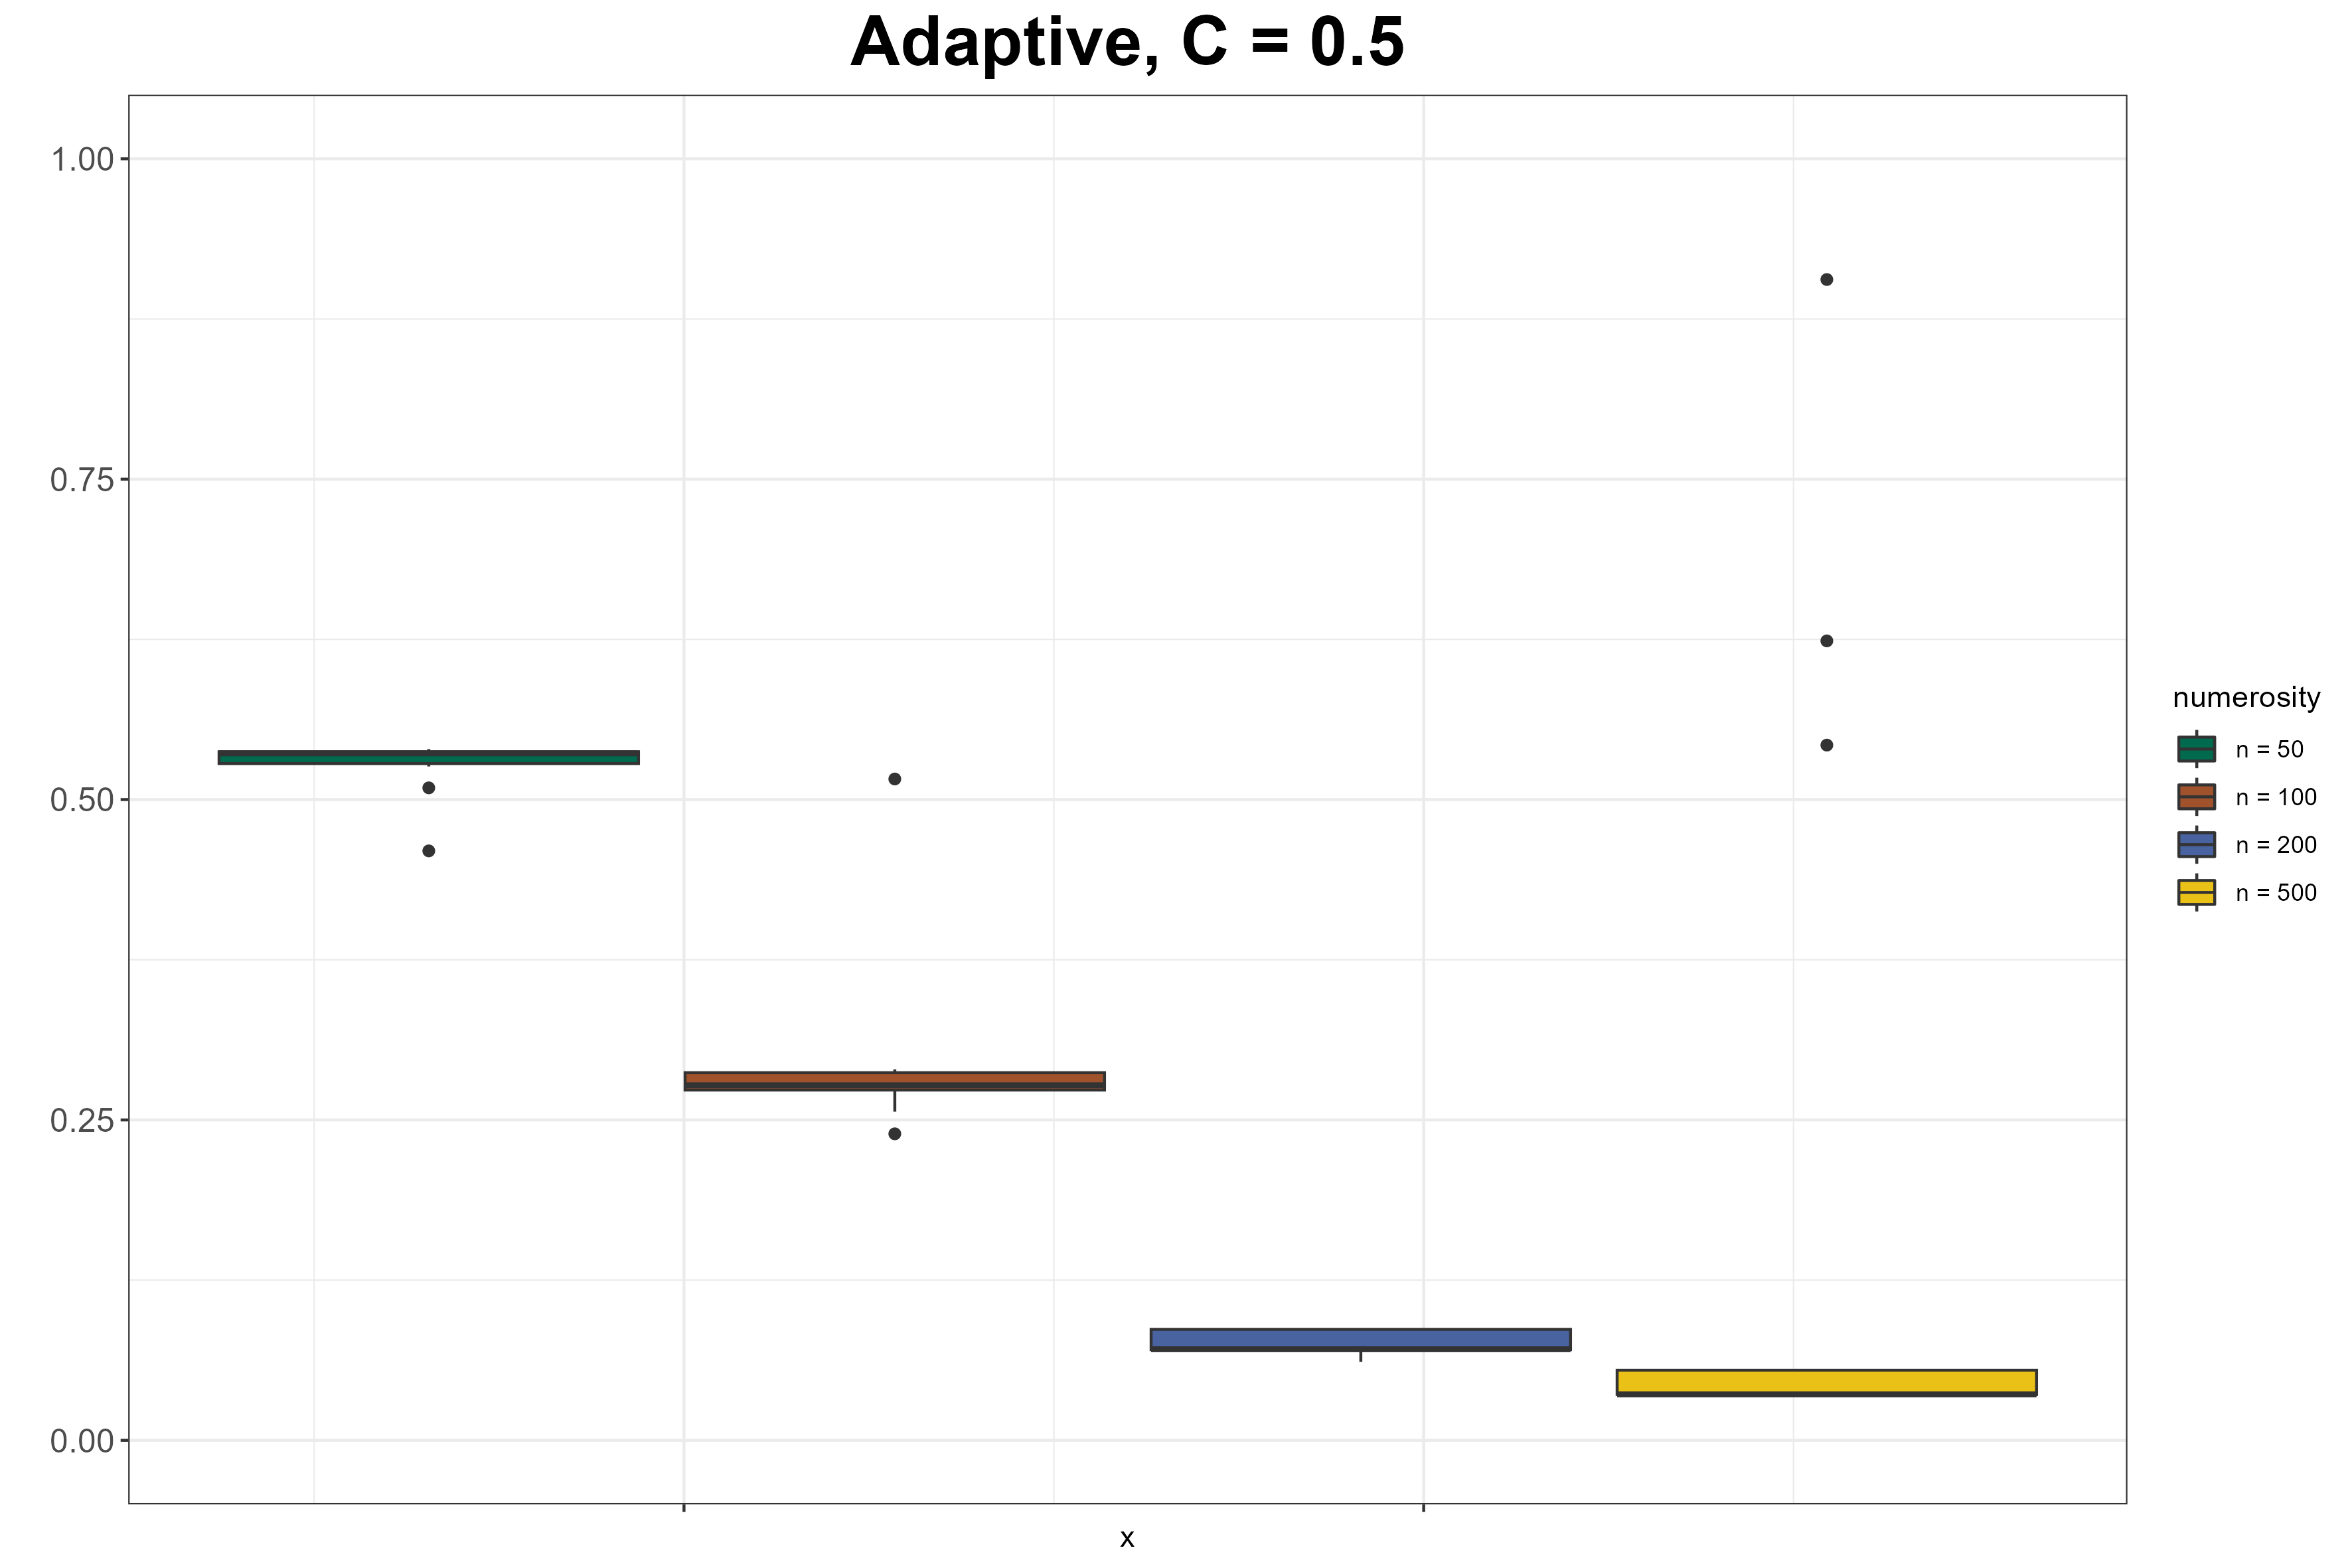
\includegraphics[height=3.5cm]{Figures/Overall_comparison/Boxplot_KL_c05.png}
				%\caption{Sample size 100}
				\label{fig:kl-100}
			\end{subfigure}
			
			\vspace{0.3cm}   % vertical space between rows 
			
			% Third figure
			\begin{subfigure}[b]{0.45\textwidth}   
				\centering
				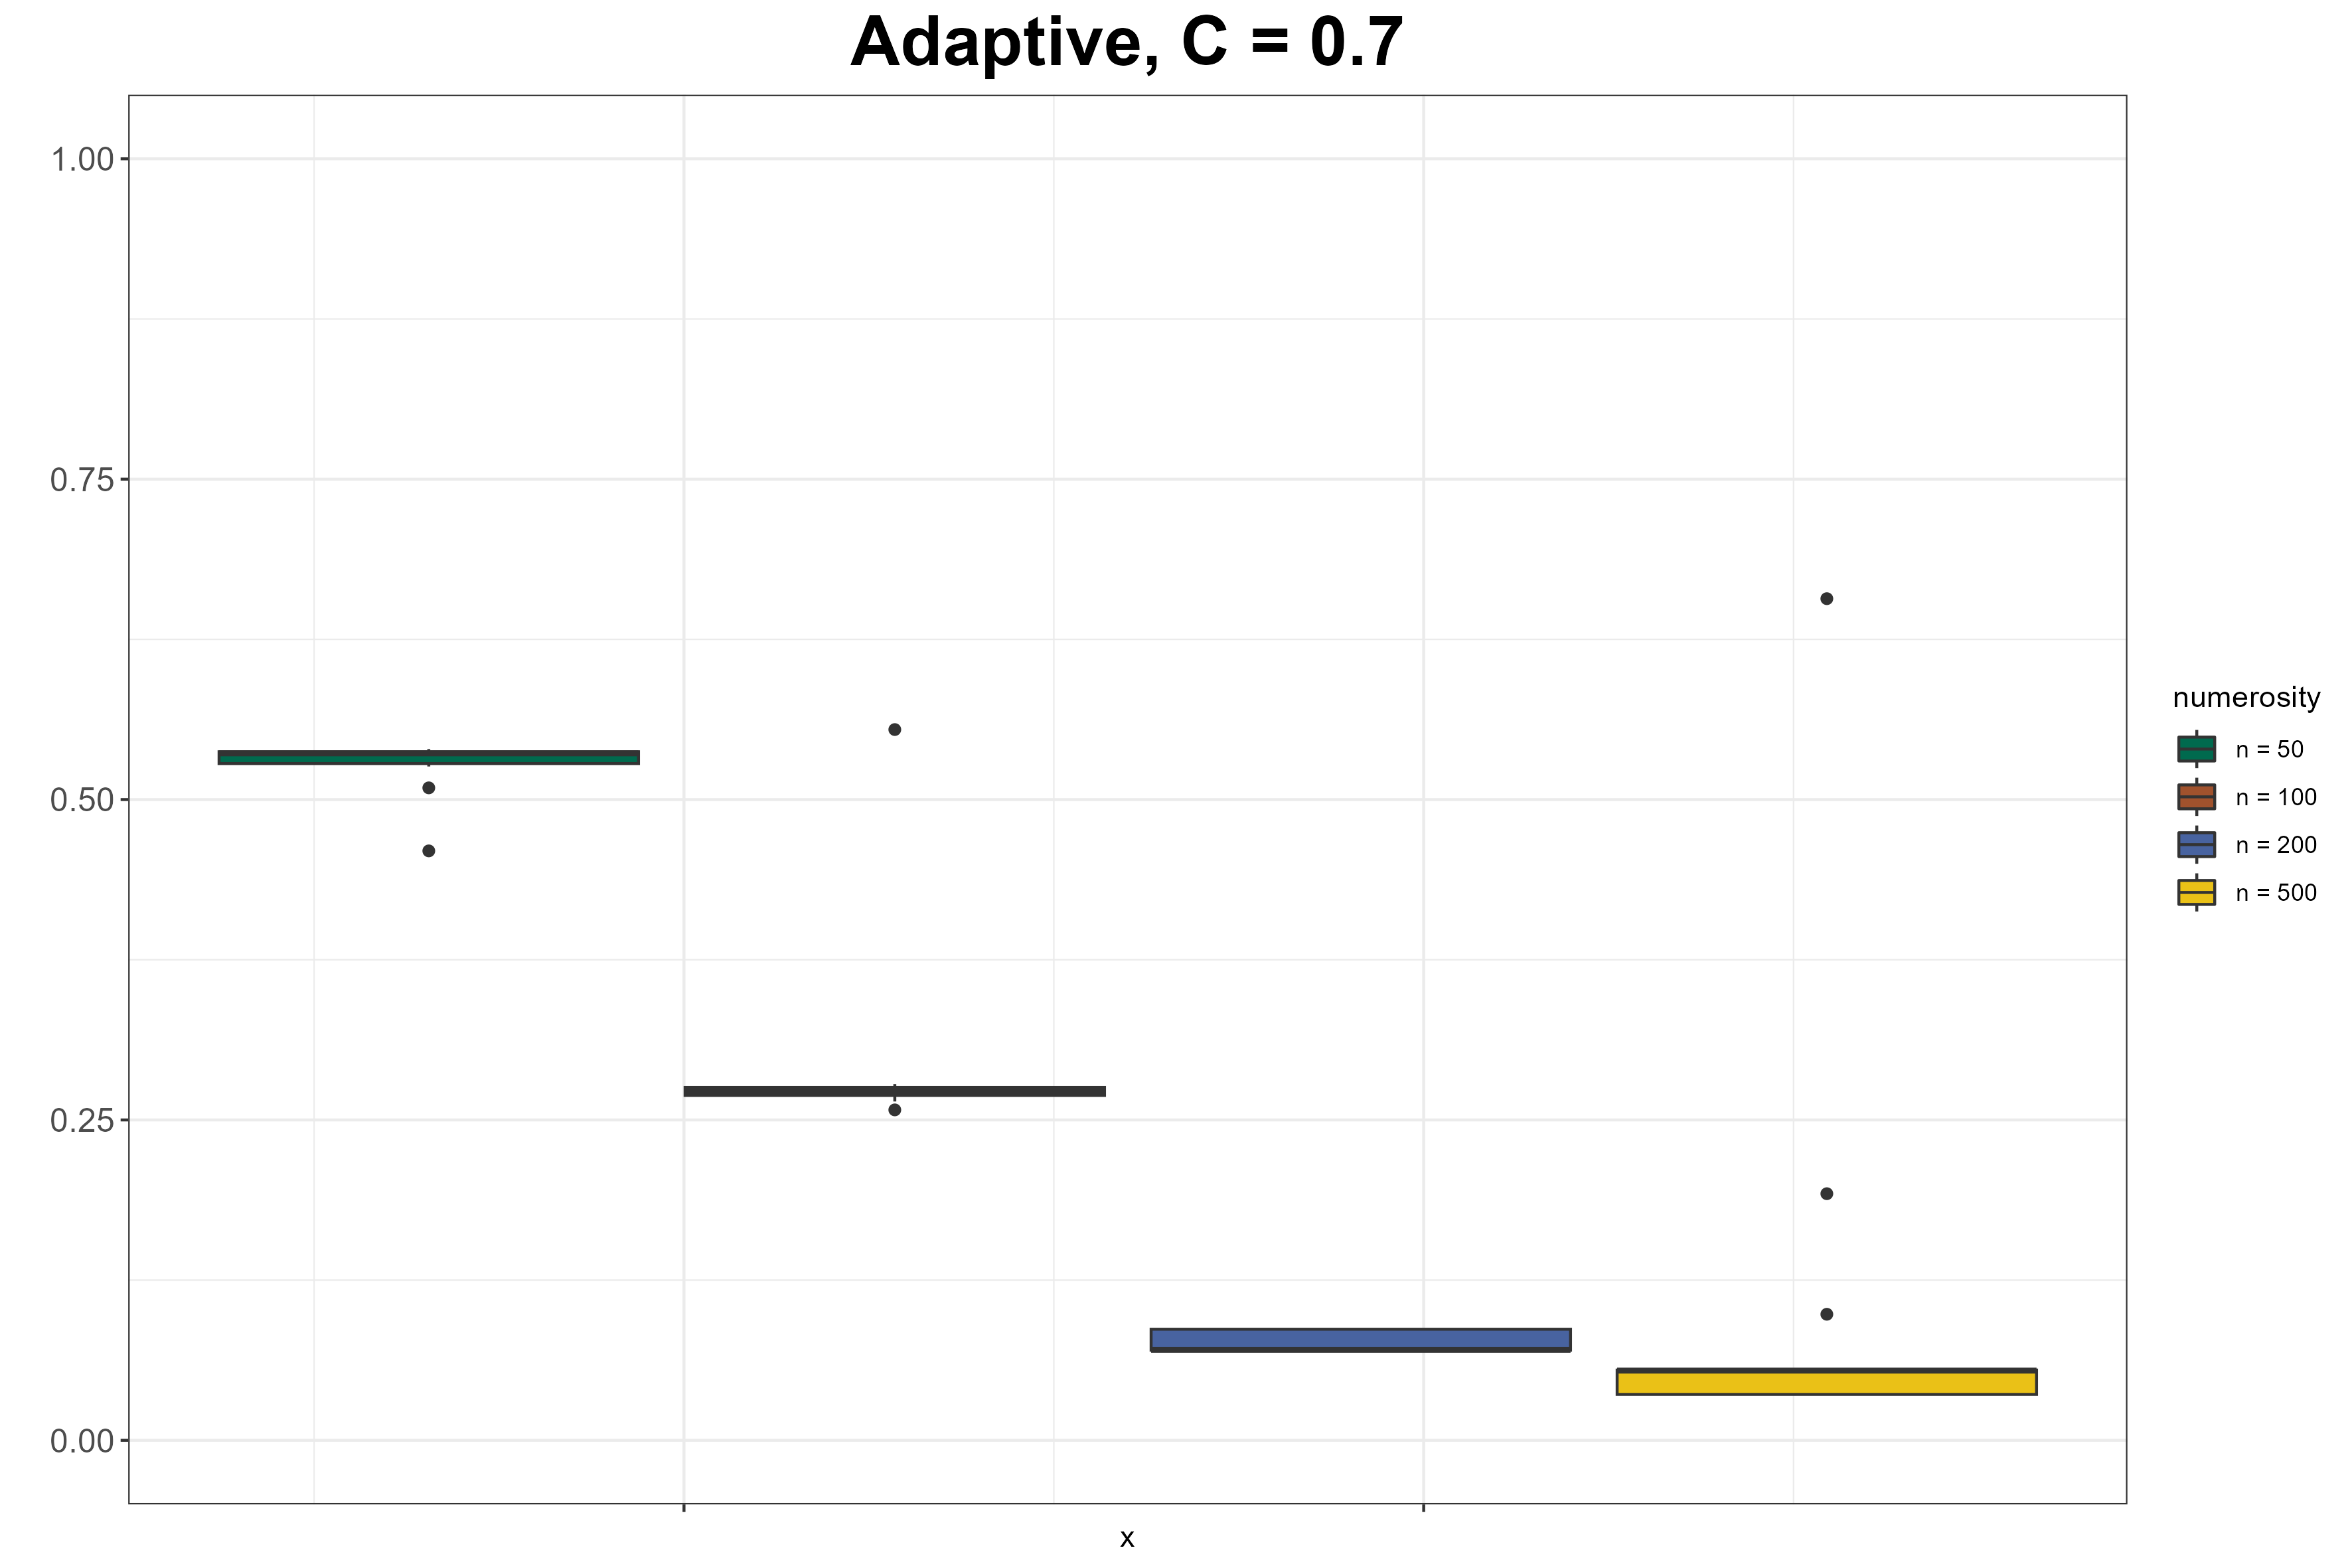
\includegraphics[height=3.5cm]{Figures/Overall_comparison/Boxplot_KL_c07.png}
				%\caption{Sample size 200}
				\label{fig:kl-200}
			\end{subfigure}
			\hspace{0.35cm}  % horizontal space between figures
			% Fourth figure
			\begin{subfigure}[b]{0.45\textwidth}   
				\centering
				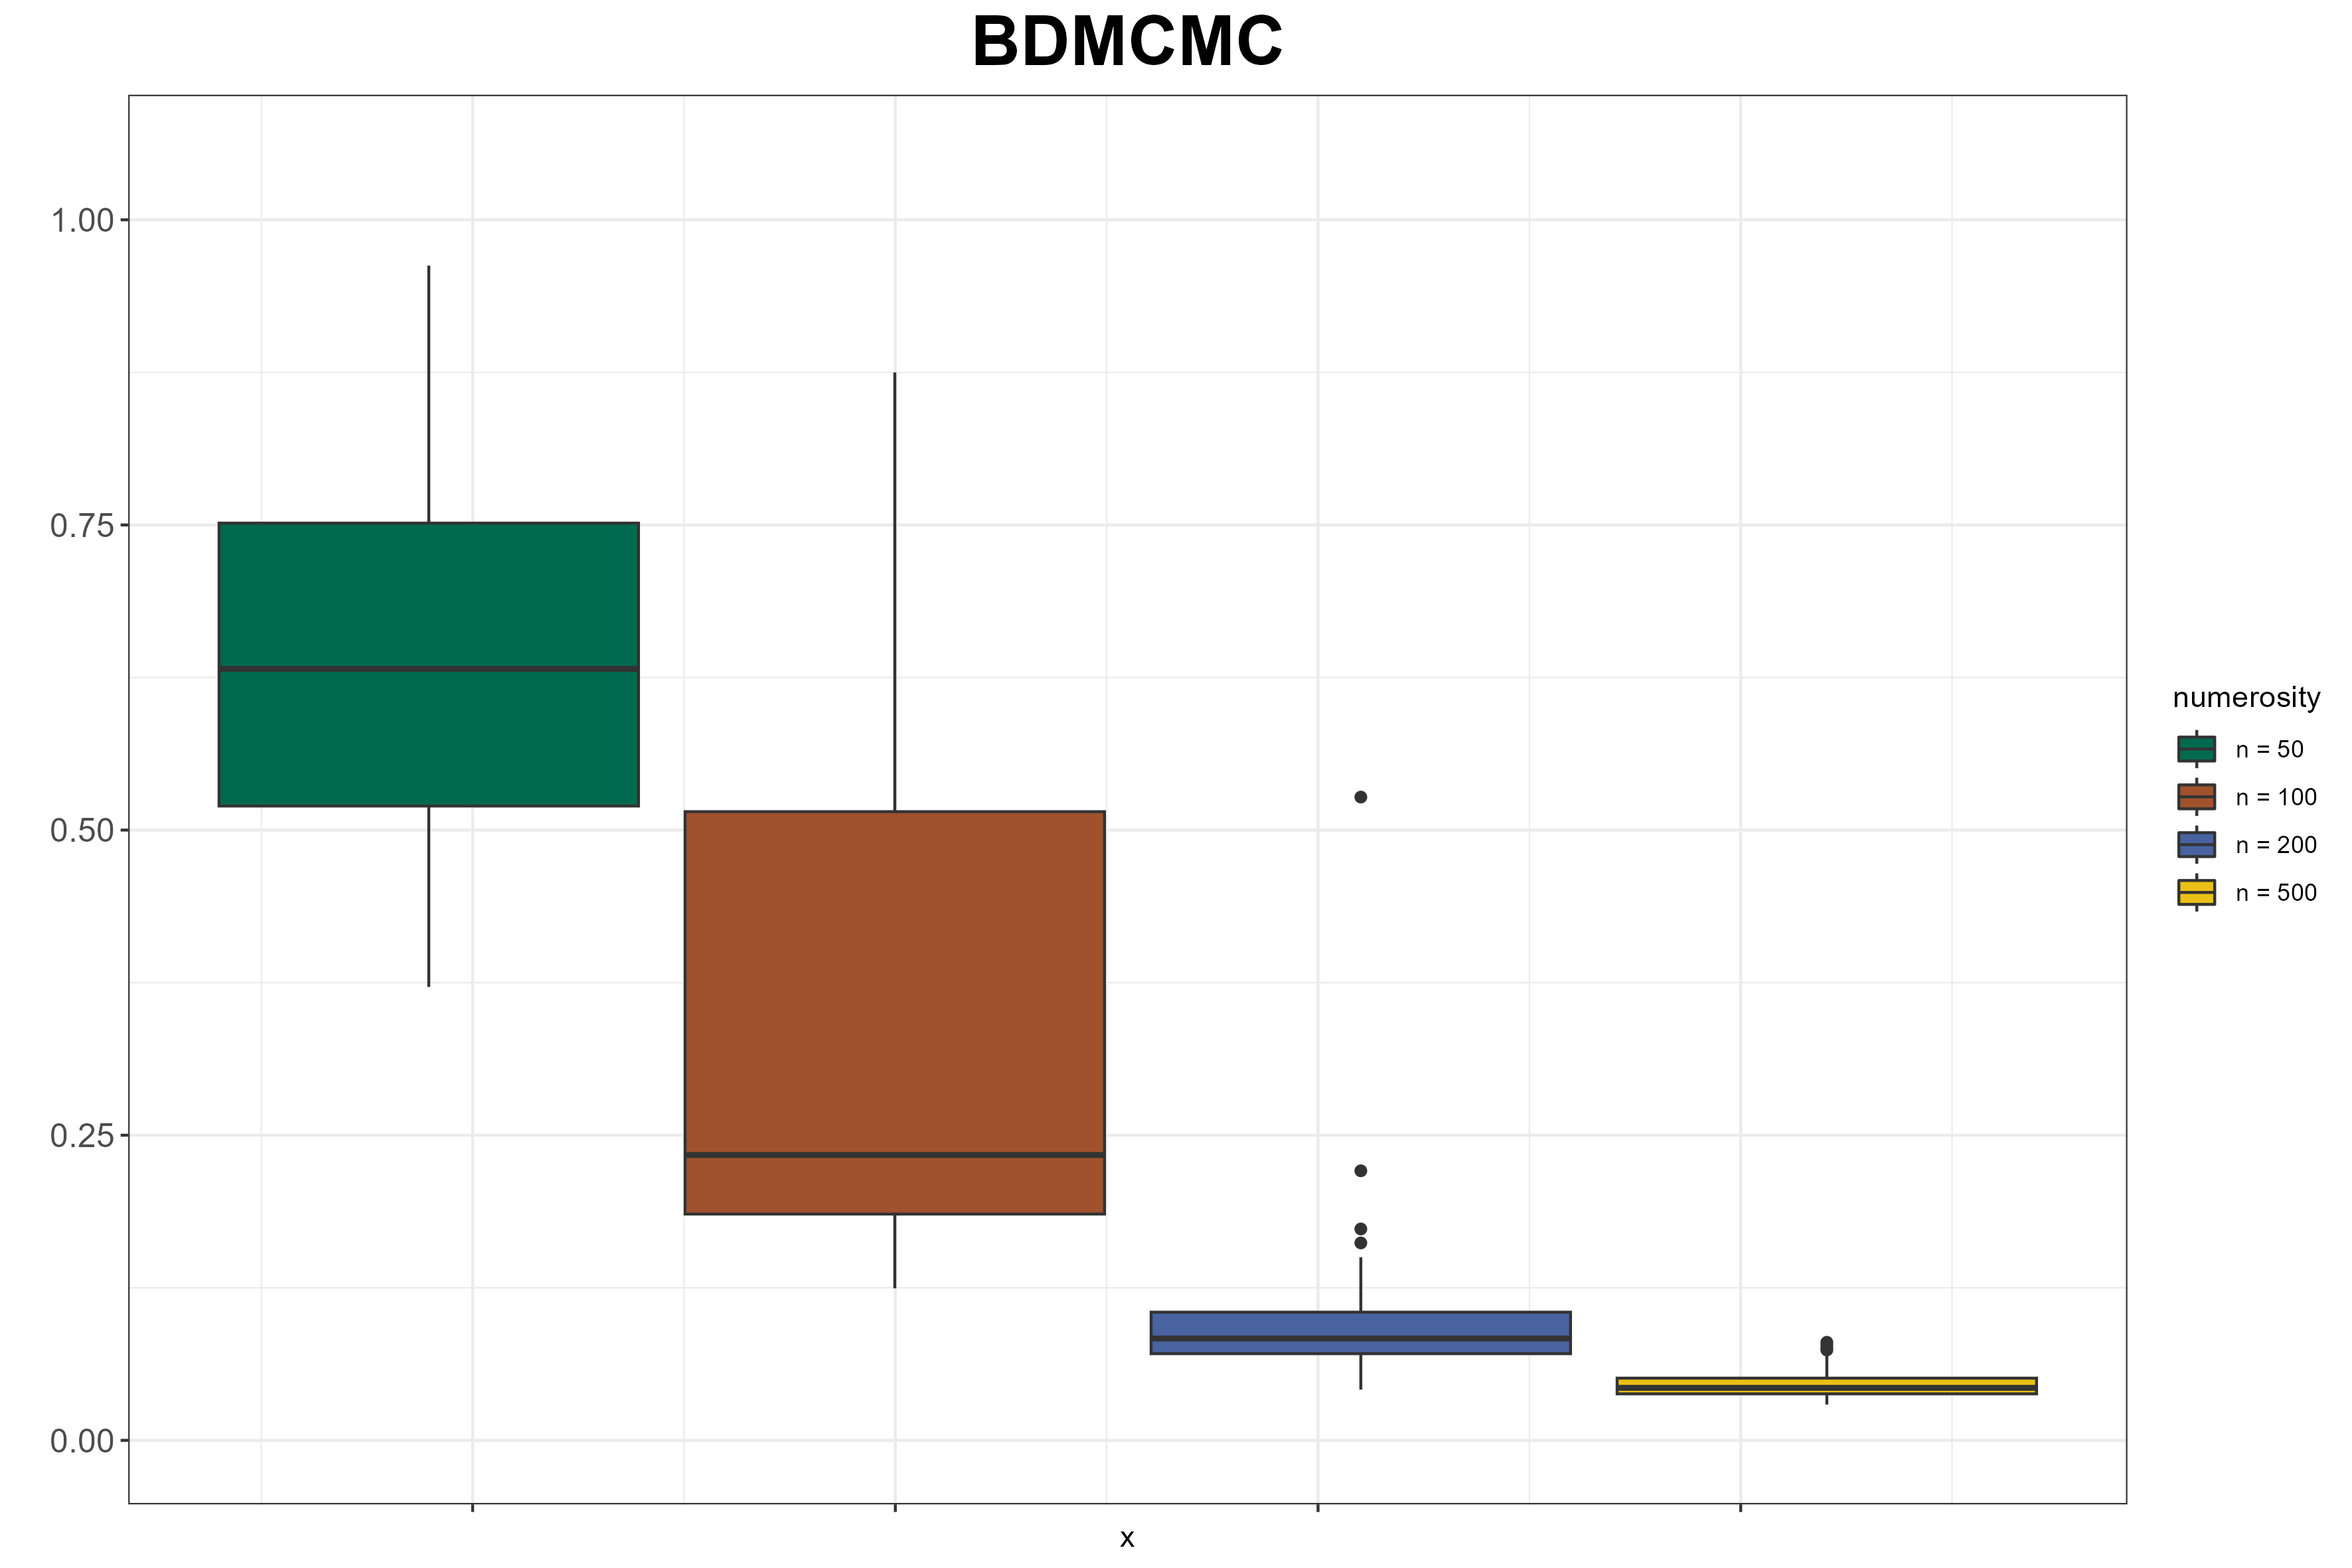
\includegraphics[height=3.5cm]{Figures/Overall_comparison/Boxplot_KL_bdmcmc.png}
				%\caption{Sample size 500}
				\label{fig:kl-500}
			\end{subfigure}
		\end{minipage}
	}
	\caption{Boxplots of Kullback-Leibler divergence from the Estimated Precision Matrix to the true Sigma across algorithms.}
	\label{fig:kl-overall}
\end{figure}

\begin{table}[!ht]
	\centering
	\begin{tabular}{|l|l|l|l|l|}
		\hline
		\textbf{} & Plain Metropolis & Adaptive, C = 0.5 & Adaptive, C = 0.7 & BDMCMC \\ \hline
		\textbf{n = 50} & 0.506 (0.026) & 0.528 (0.02) & 0.528 (0.02) & 0.639 (0.15) \\ \hline
		\textbf{n = 100} & 0.404 (0.252) & 0.291 (0.064) & 0.29 (0.073) & 0.332 (0.213) \\ \hline
		\textbf{n = 200} & 0.104 (0.098) & 0.077 (0.008) & 0.077 (0.008) & 0.101 (0.07) \\ \hline
		\textbf{n = 500} & 0.242 (0.311) & 0.172 (0.278) & 0.098 (0.16) & 0.047 (0.012) \\ \hline
	\end{tabular}
	\caption{Kullback-Leibler divergence from the Estimated Correlation Matrix to the true Sigma across algorithms together with standard errors (in parenthesis).}
	\label{table:Kullback-leibler}
\end{table}

\subsubsection{Structural Hamming distance}

Structural Hamming Distance summaries are shown in \textit{Figure} \ref{fig:shd}, illustrating a general trend of improvement across all algorithms as the sample size increases. The BDMCMC exhibits the highest error at a sample size of 50, while the plain Metropolis and the adaptive algorithm with $C = 0.5$ show similar instability at a sample size of 100. Despite these variations at smaller sample sizes, all four algorithms demonstrate the ability to recover the true graph structure as the sample size grows, with errors stabilizing around two for larger samples.

\begin{figure}[h] 
	\centering
	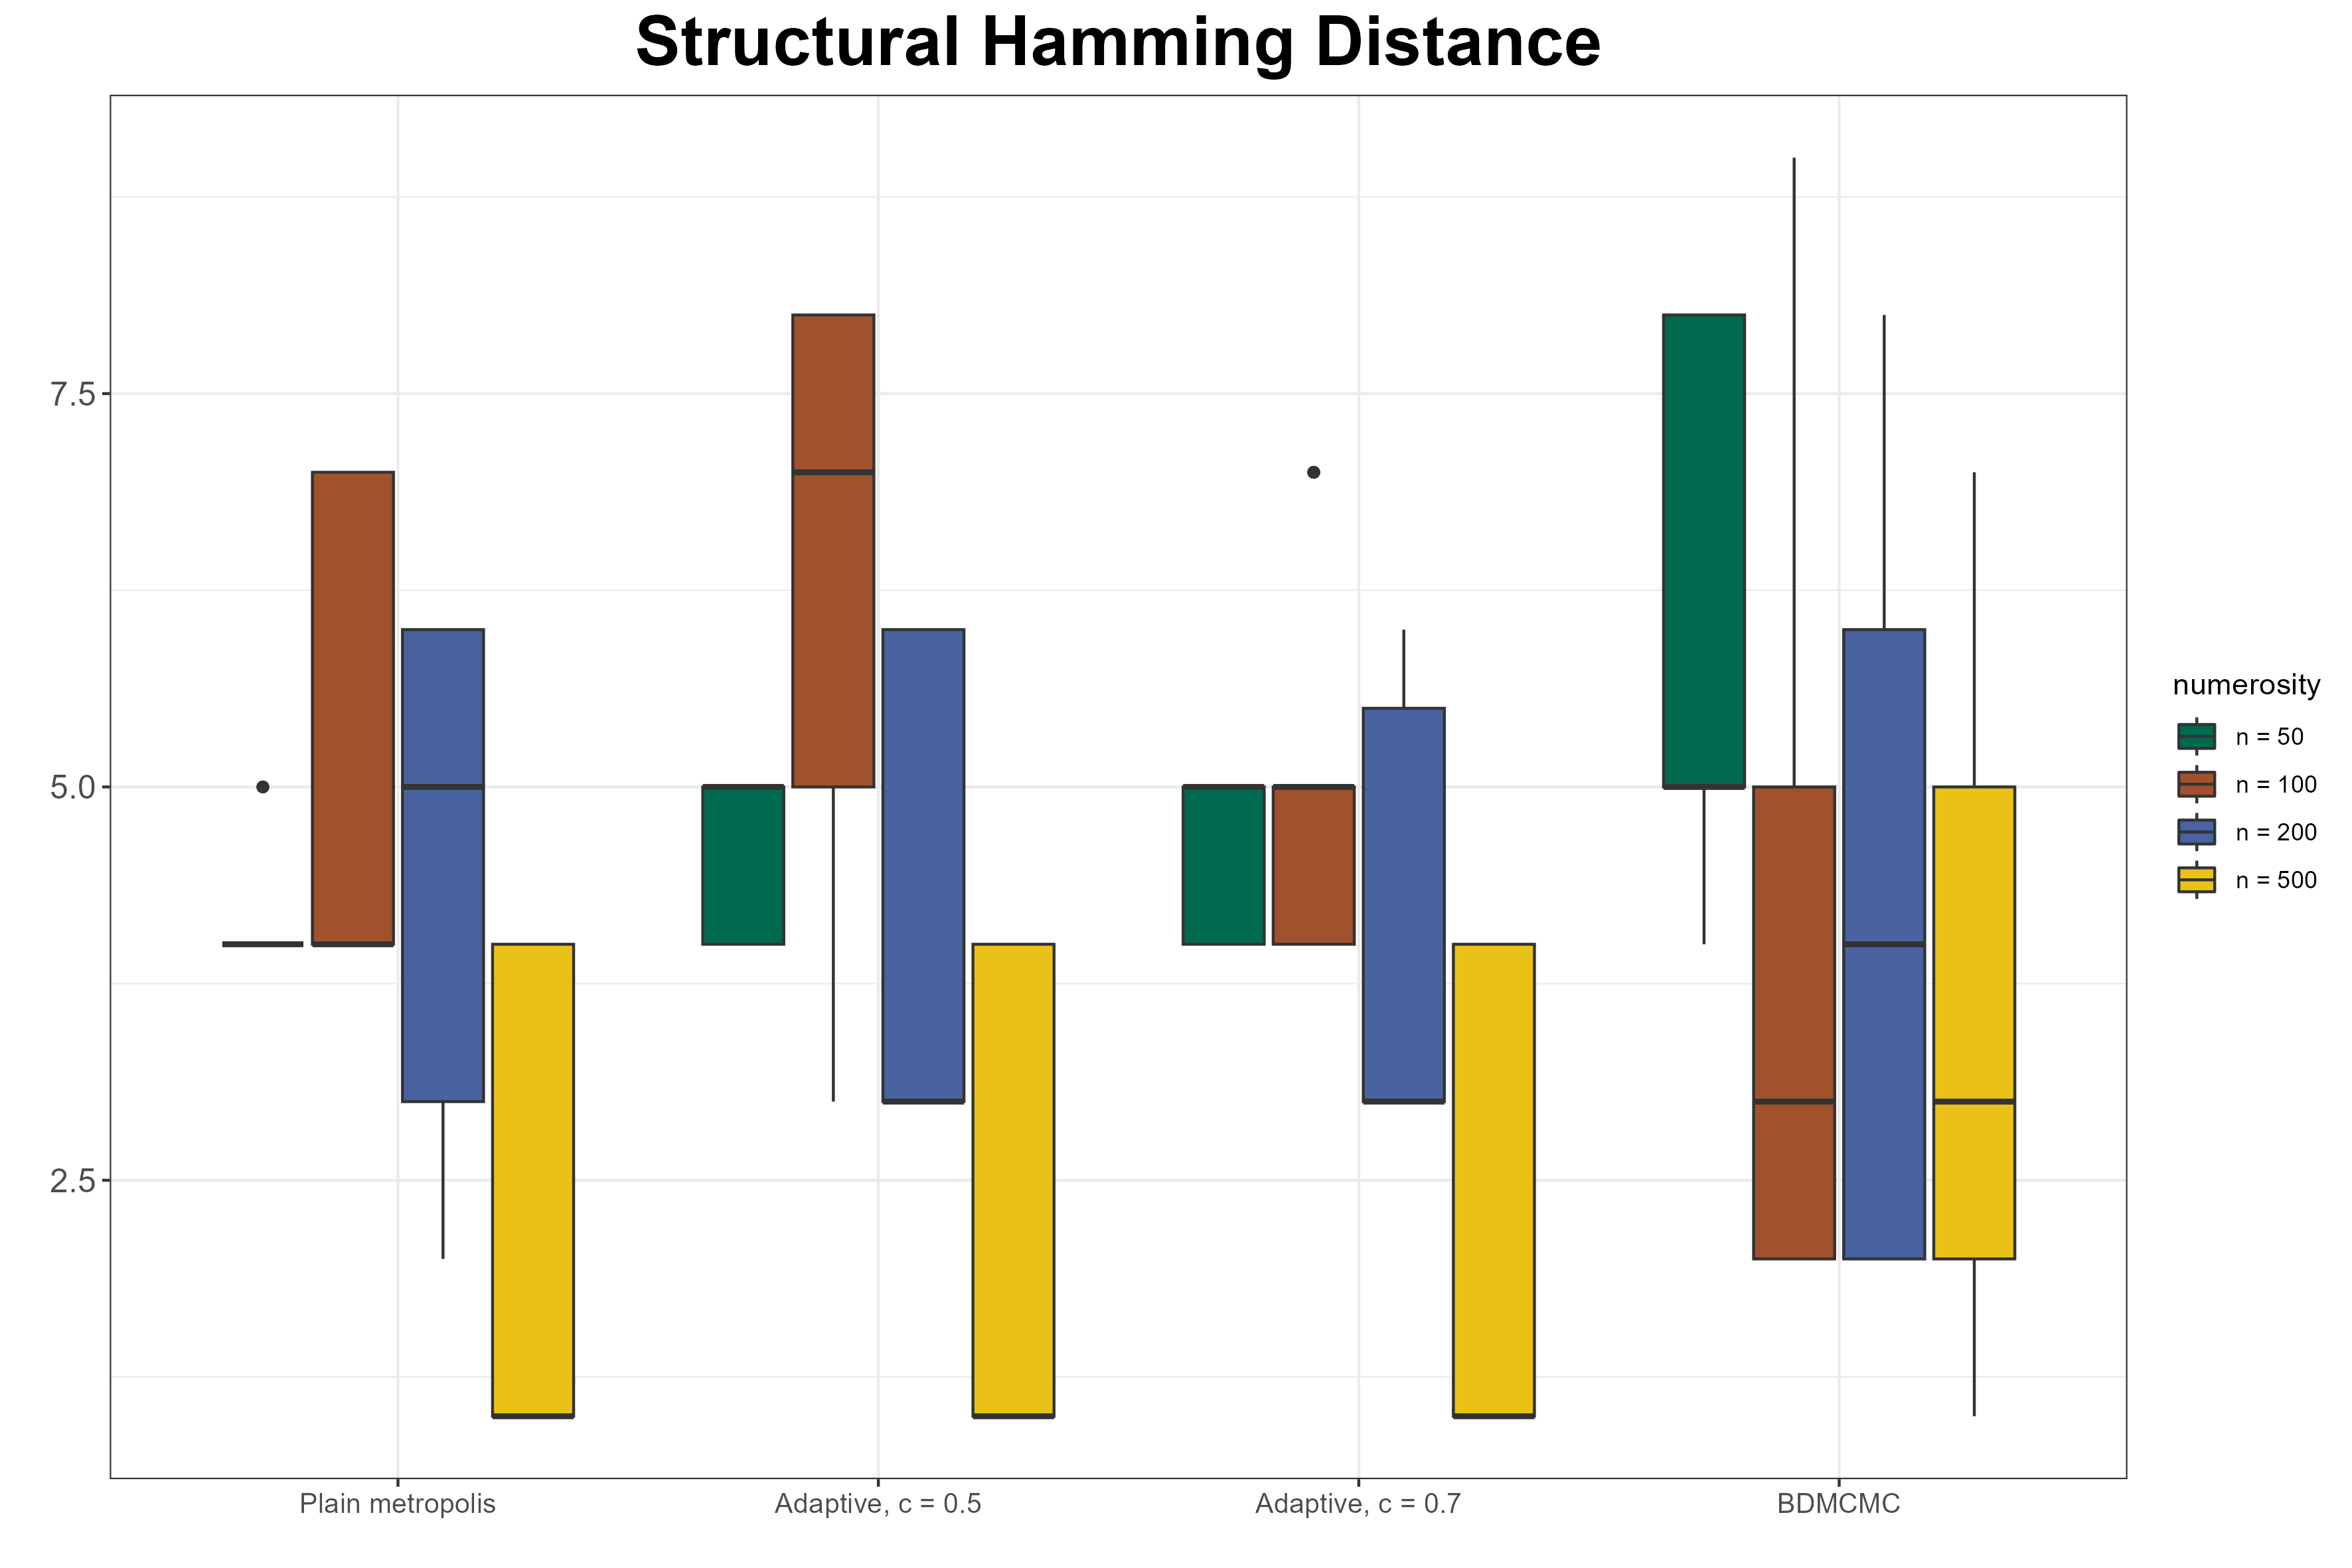
\includegraphics[width=0.8\textwidth]{Figures/Overall_comparison/Boxplot_shd.png}
	\caption{Boxplot of Structural Hamming Distance across algorithms}
	\label{fig:shd}
\end{figure}

\section{Convergence Assessment Using Random DAGs}

To evaluate the convergence of the chains, 15 independent simulations were conducted for three different sample sizes: $n = 200, 500,$ and $1000$. In each simulation, a set of random DAGs was generated, and the same dataset was used across all runs of the algorithm to ensure a fair comparison of their performance. Adaptive metropolis has, in this context, parameter C equal to 0.5.
By utilizing random DAGs instead of a single true structure, the analysis introduces an additional layer of complexity. Specifically, the algorithms are not only tasked with identifying the correct edges but must also capture the broader Markov equivalence class that defines the true underlying structure. 

\subsection{Heatmap Visualization of Results}

In \textit{Figures} \ref{fig: one-two-dags} and \ref{fig: two-three-dags}, the overall convergence behavior of the algorithms is visualized. The heatmaps illustrate the average edge inclusion probabilities, calculated across multiple replicates for each algorithm and sample size. To account for the equivalence of DAGs under the same Markov equivalence class, symmetric edges are also incorporated, as they reflect the shared statistical properties of the true graph structure.

The results show that all three algorithms converge toward the target DAG structure, with the plain and adaptive Metropolis  algorithms displaying a more precise characterization of the final selected edges, as evidenced by lower uncertainty in their edge probabilities. In contrast, the Birth-Death MCMC algorithm reveals a higher degree of uncertainty in the final configuration. This discrepancy is attributed to the smaller number of unique DAGs sampled per replicate and the increased risk of the algorithm getting trapped in local optima. 

\begin{figure}[!ht]
	\centering
	\resizebox{\textwidth}{6.5cm}{  
		\begin{minipage}{\textwidth}
			\centering
			
			% First figure
			\begin{subfigure}[b]{0.45\textwidth}   
				\centering
				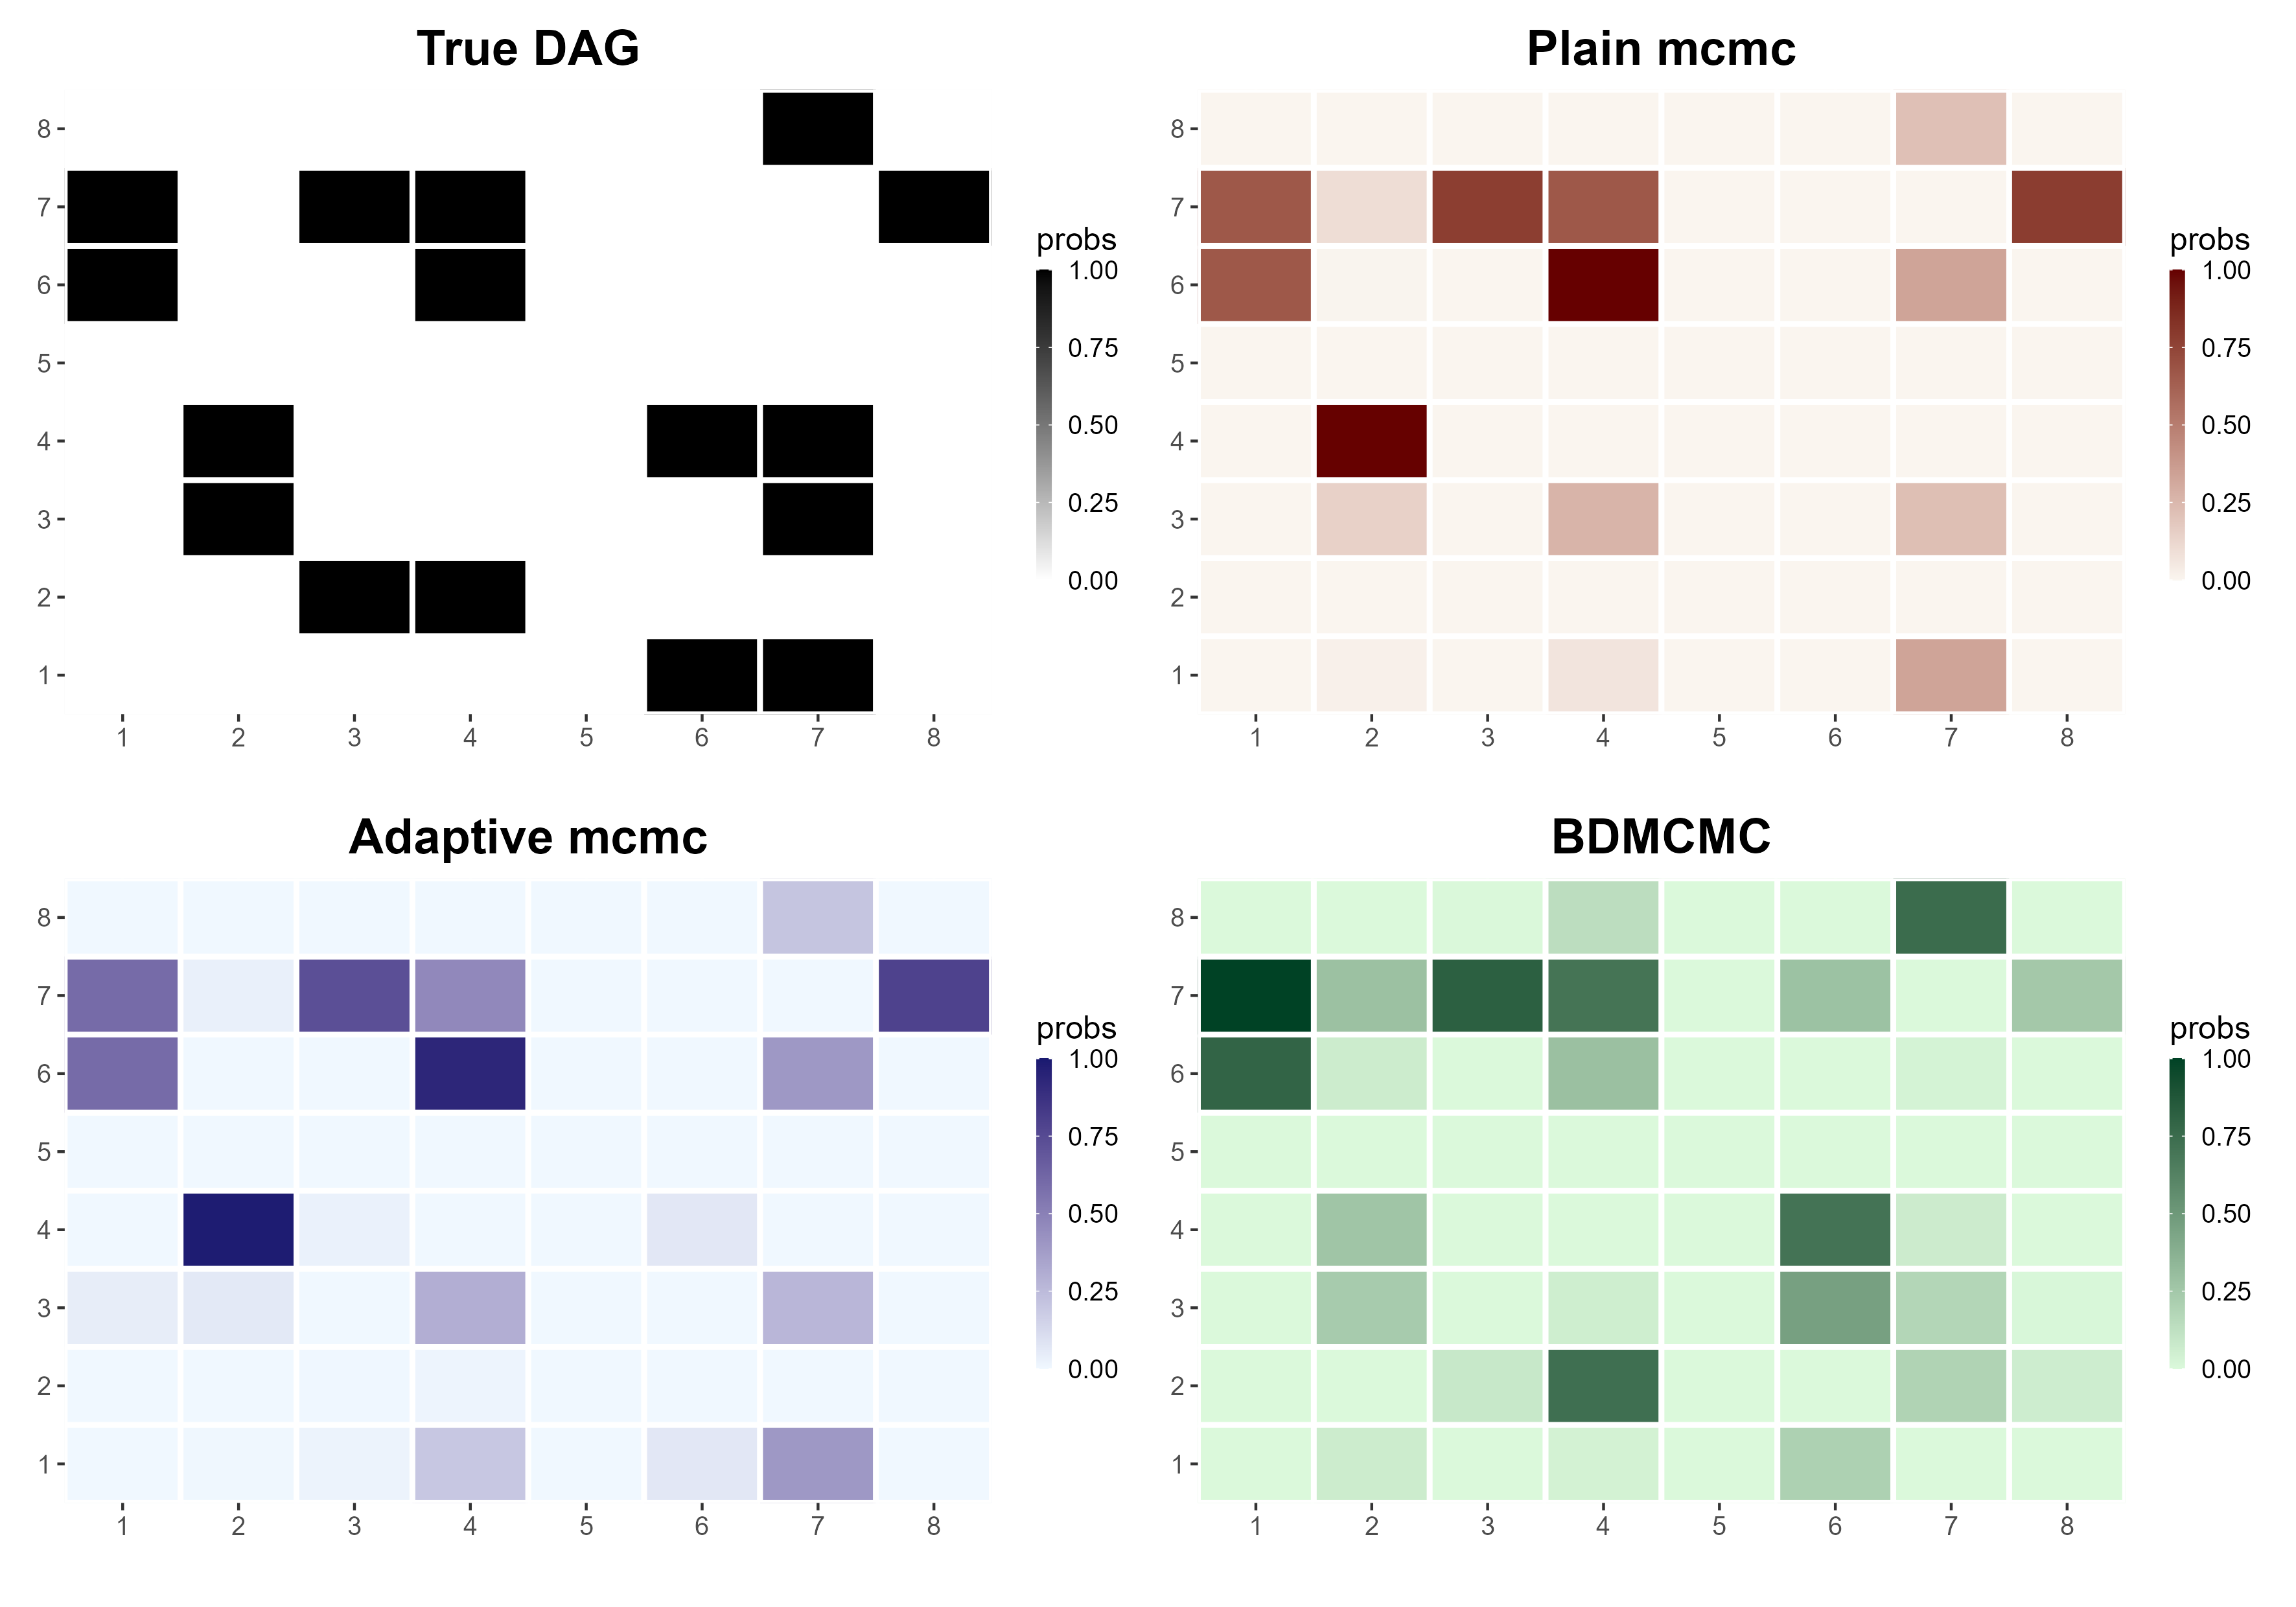
\includegraphics[width=\textwidth, height=12cm]{Figures/Overall_comparison/Random_dags/heat_dag_1_n_200.png}
				\caption{Sample size 200}
				%\label{fig:heatmaps-50}
			\end{subfigure}
			\hspace{0.35cm}  % horizontal space between figures
			% Second figure
			\begin{subfigure}[b]{0.45\textwidth}   
				\centering
				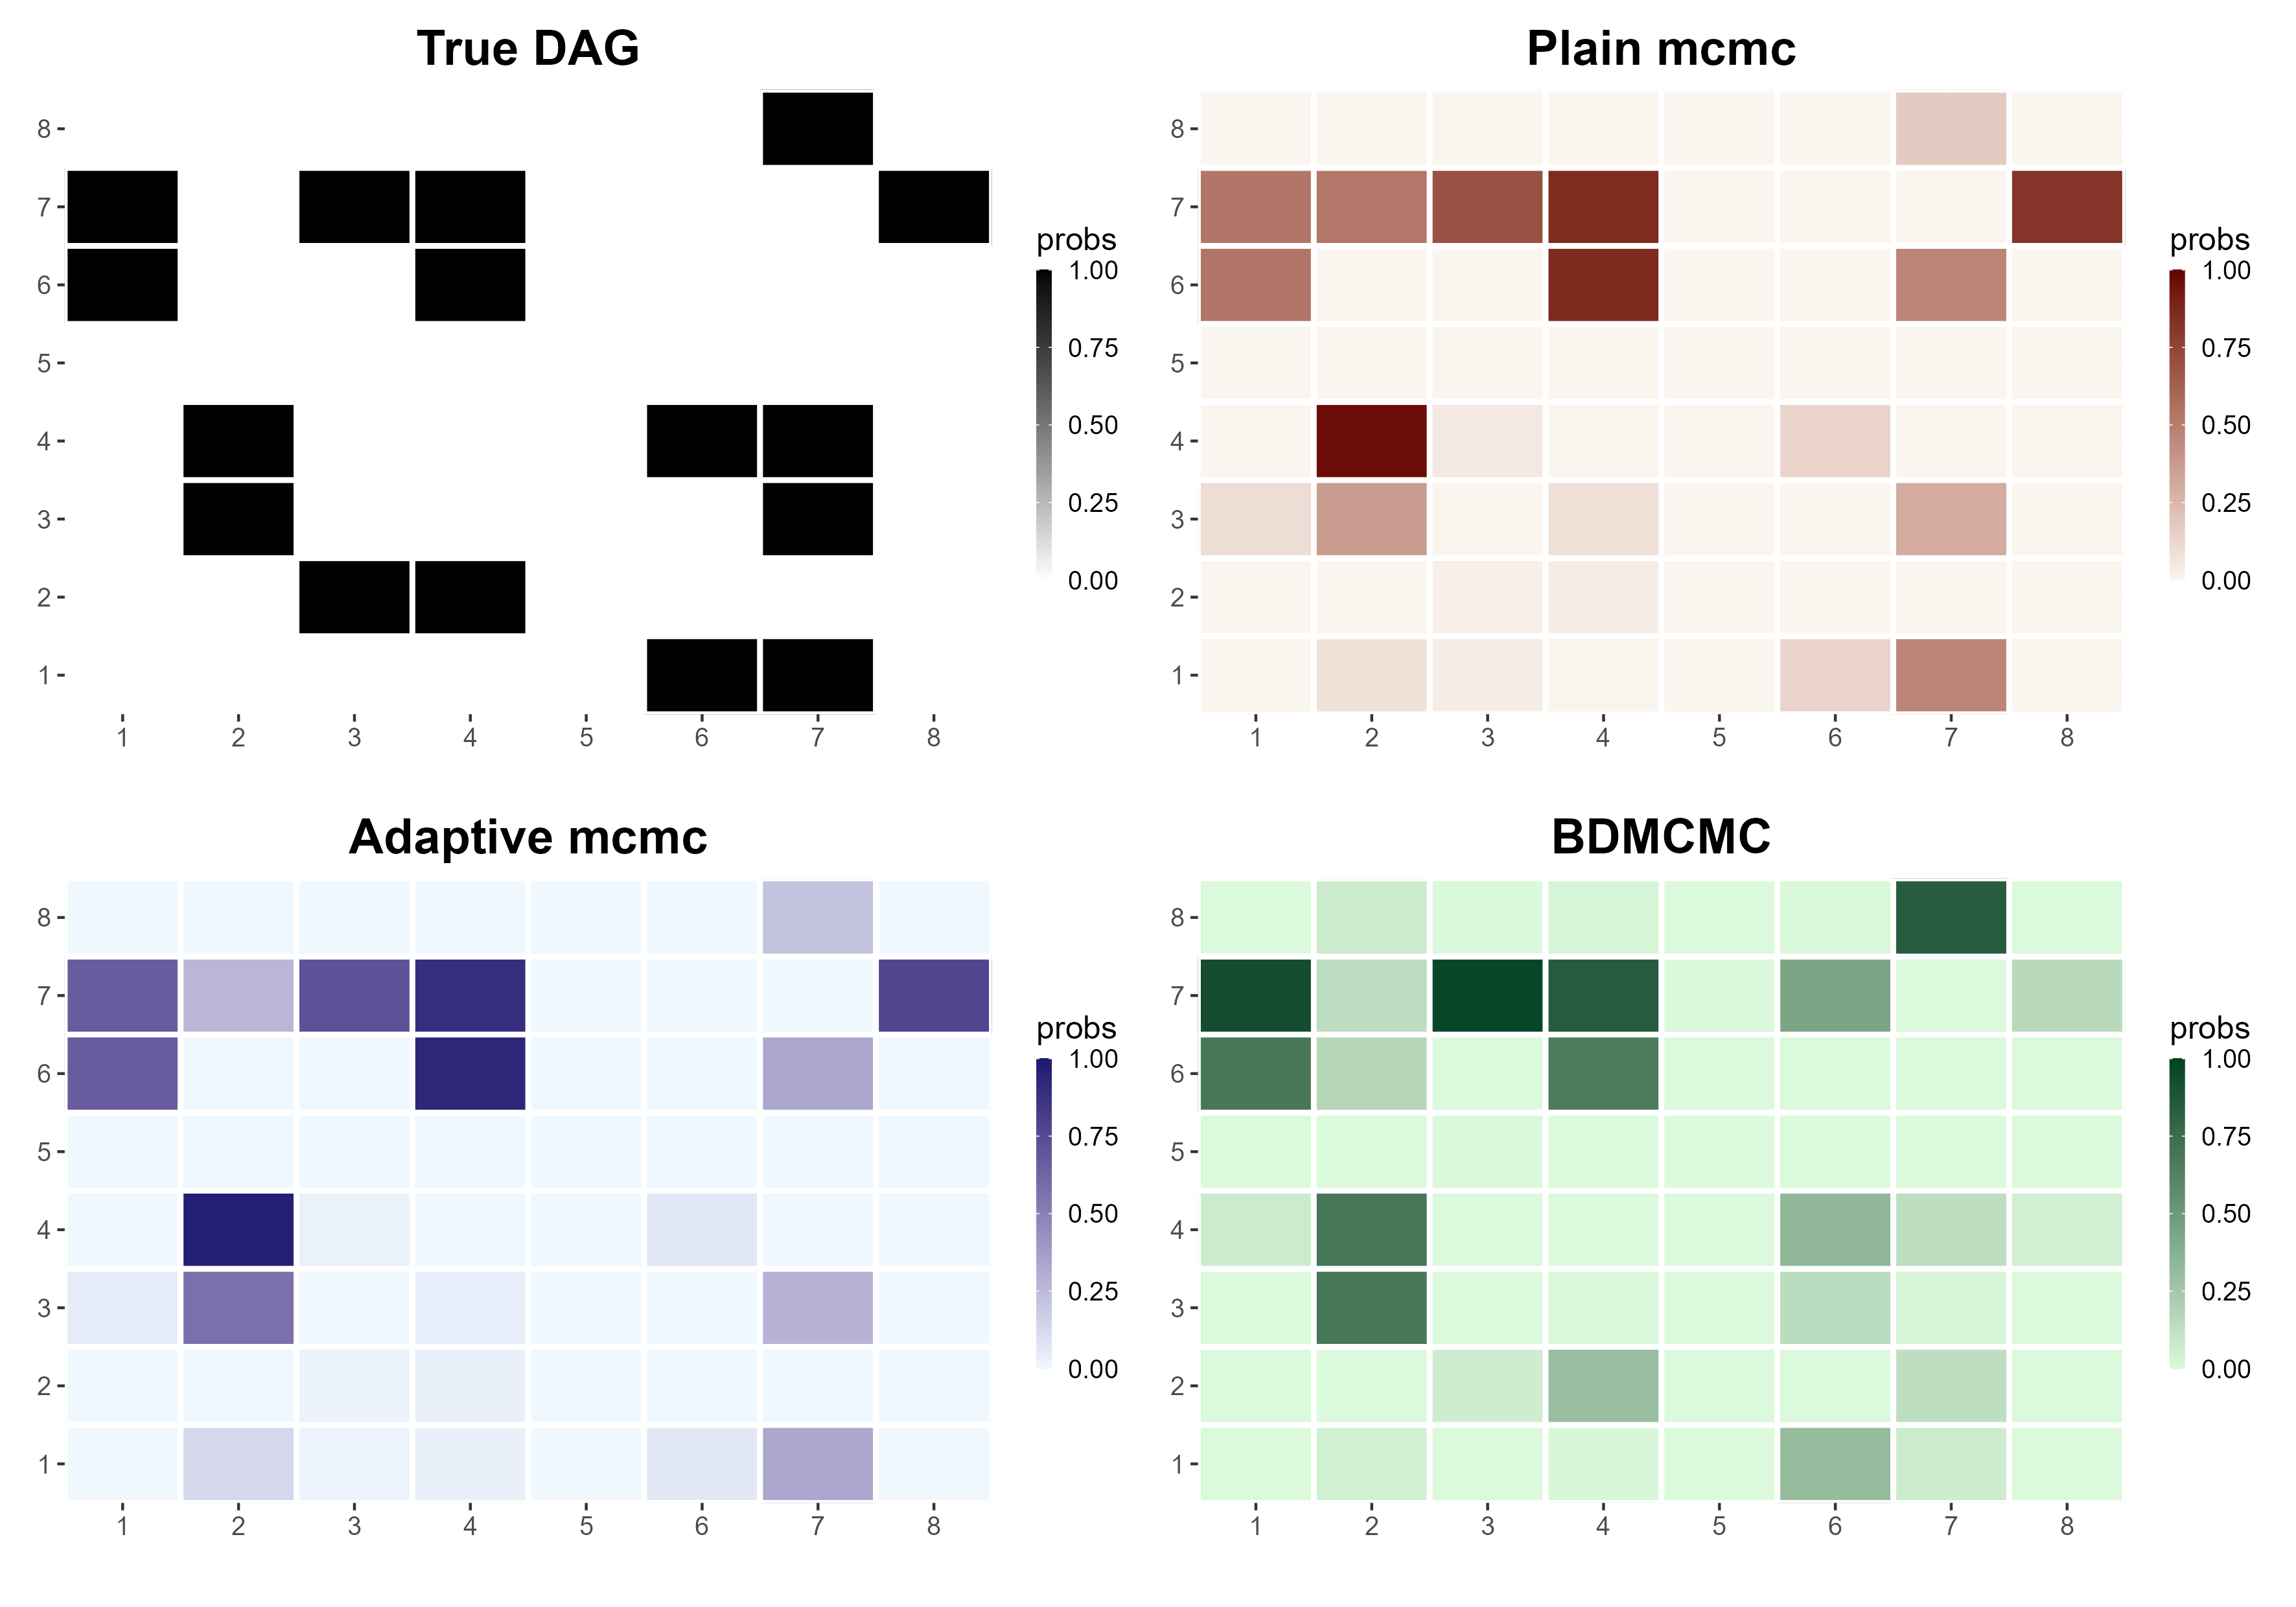
\includegraphics[width=\textwidth, height=12cm]{Figures/Overall_comparison/Random_dags/heat_dag_1_n_500.png}
				%\caption{Sample size 500}
				\label{fig:heatmaps-100}
			\end{subfigure}
			\hspace{0.35cm}
			\begin{subfigure}[b]{0.45\textwidth}   
				\centering
				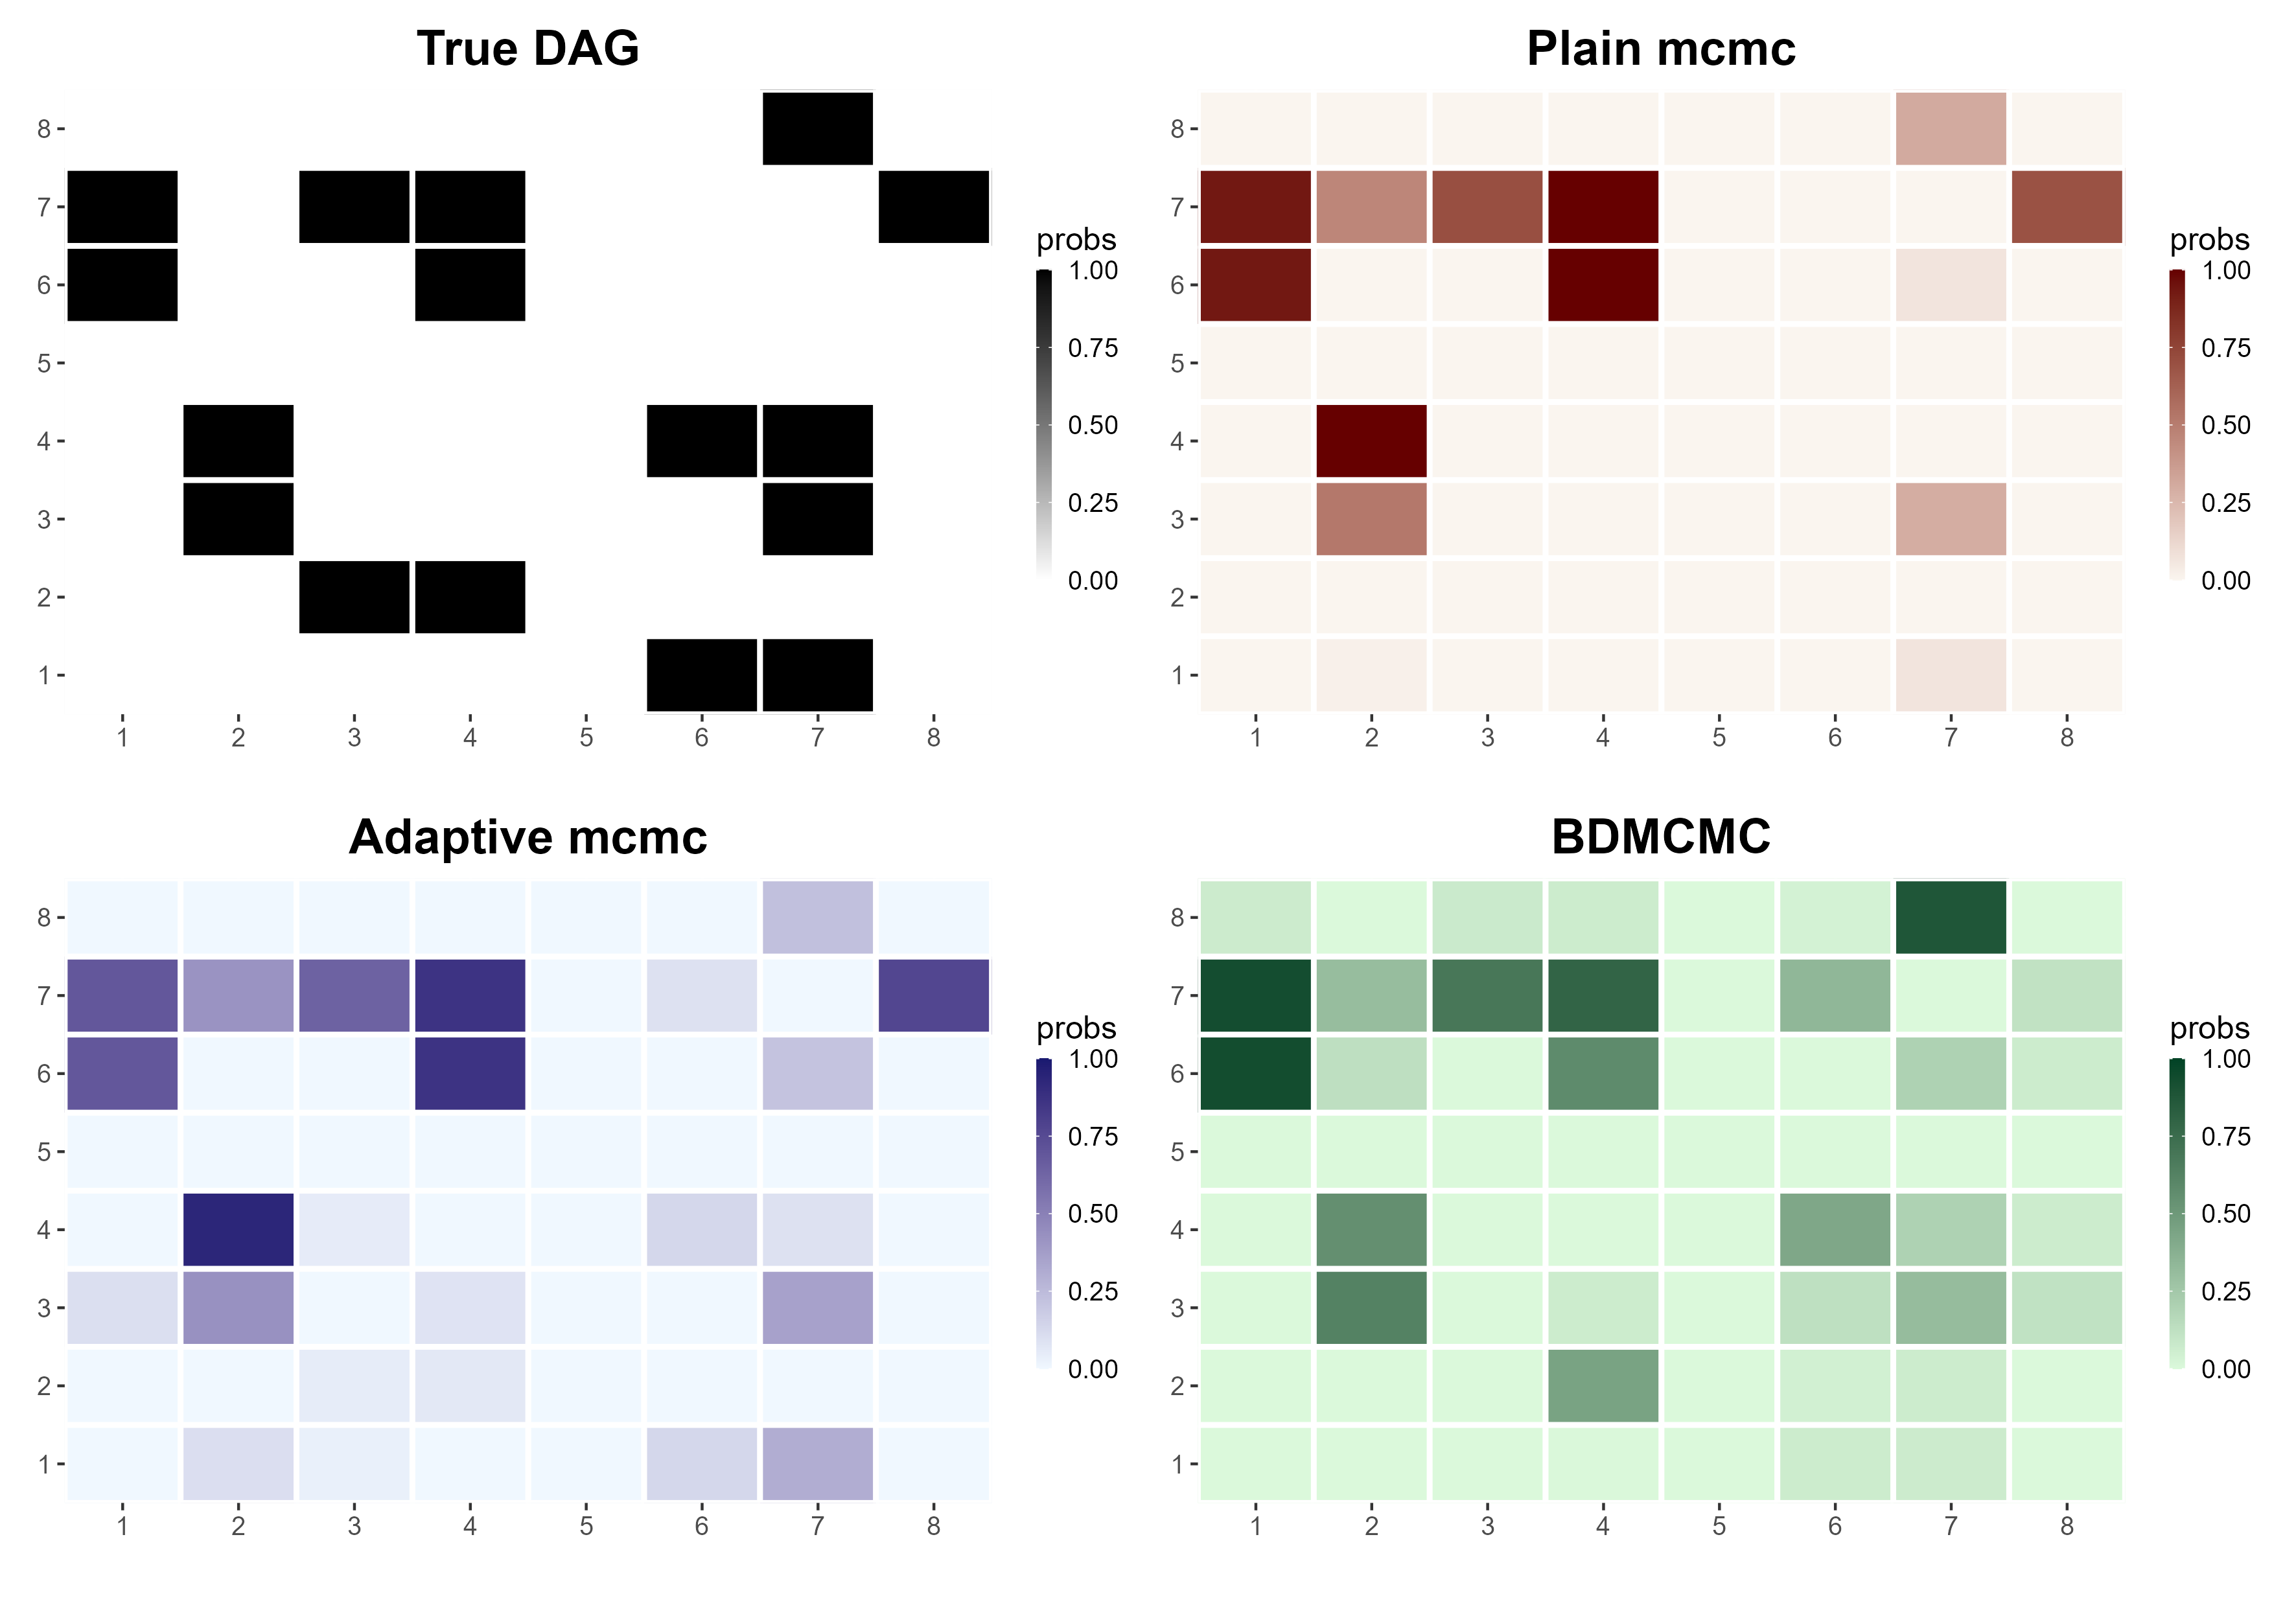
\includegraphics[width=\textwidth, height=12cm]{Figures/Overall_comparison/Random_dags/heat_dag_1_n_1000.png}
				%\caption{Sample size 1000}
				\label{fig:heatmaps-100}
			\end{subfigure}
			
			\vspace{0.4cm}   %  vertical space between rows 
			
			% Third figure
			\begin{subfigure}[b]{0.45\textwidth}   
				\centering
				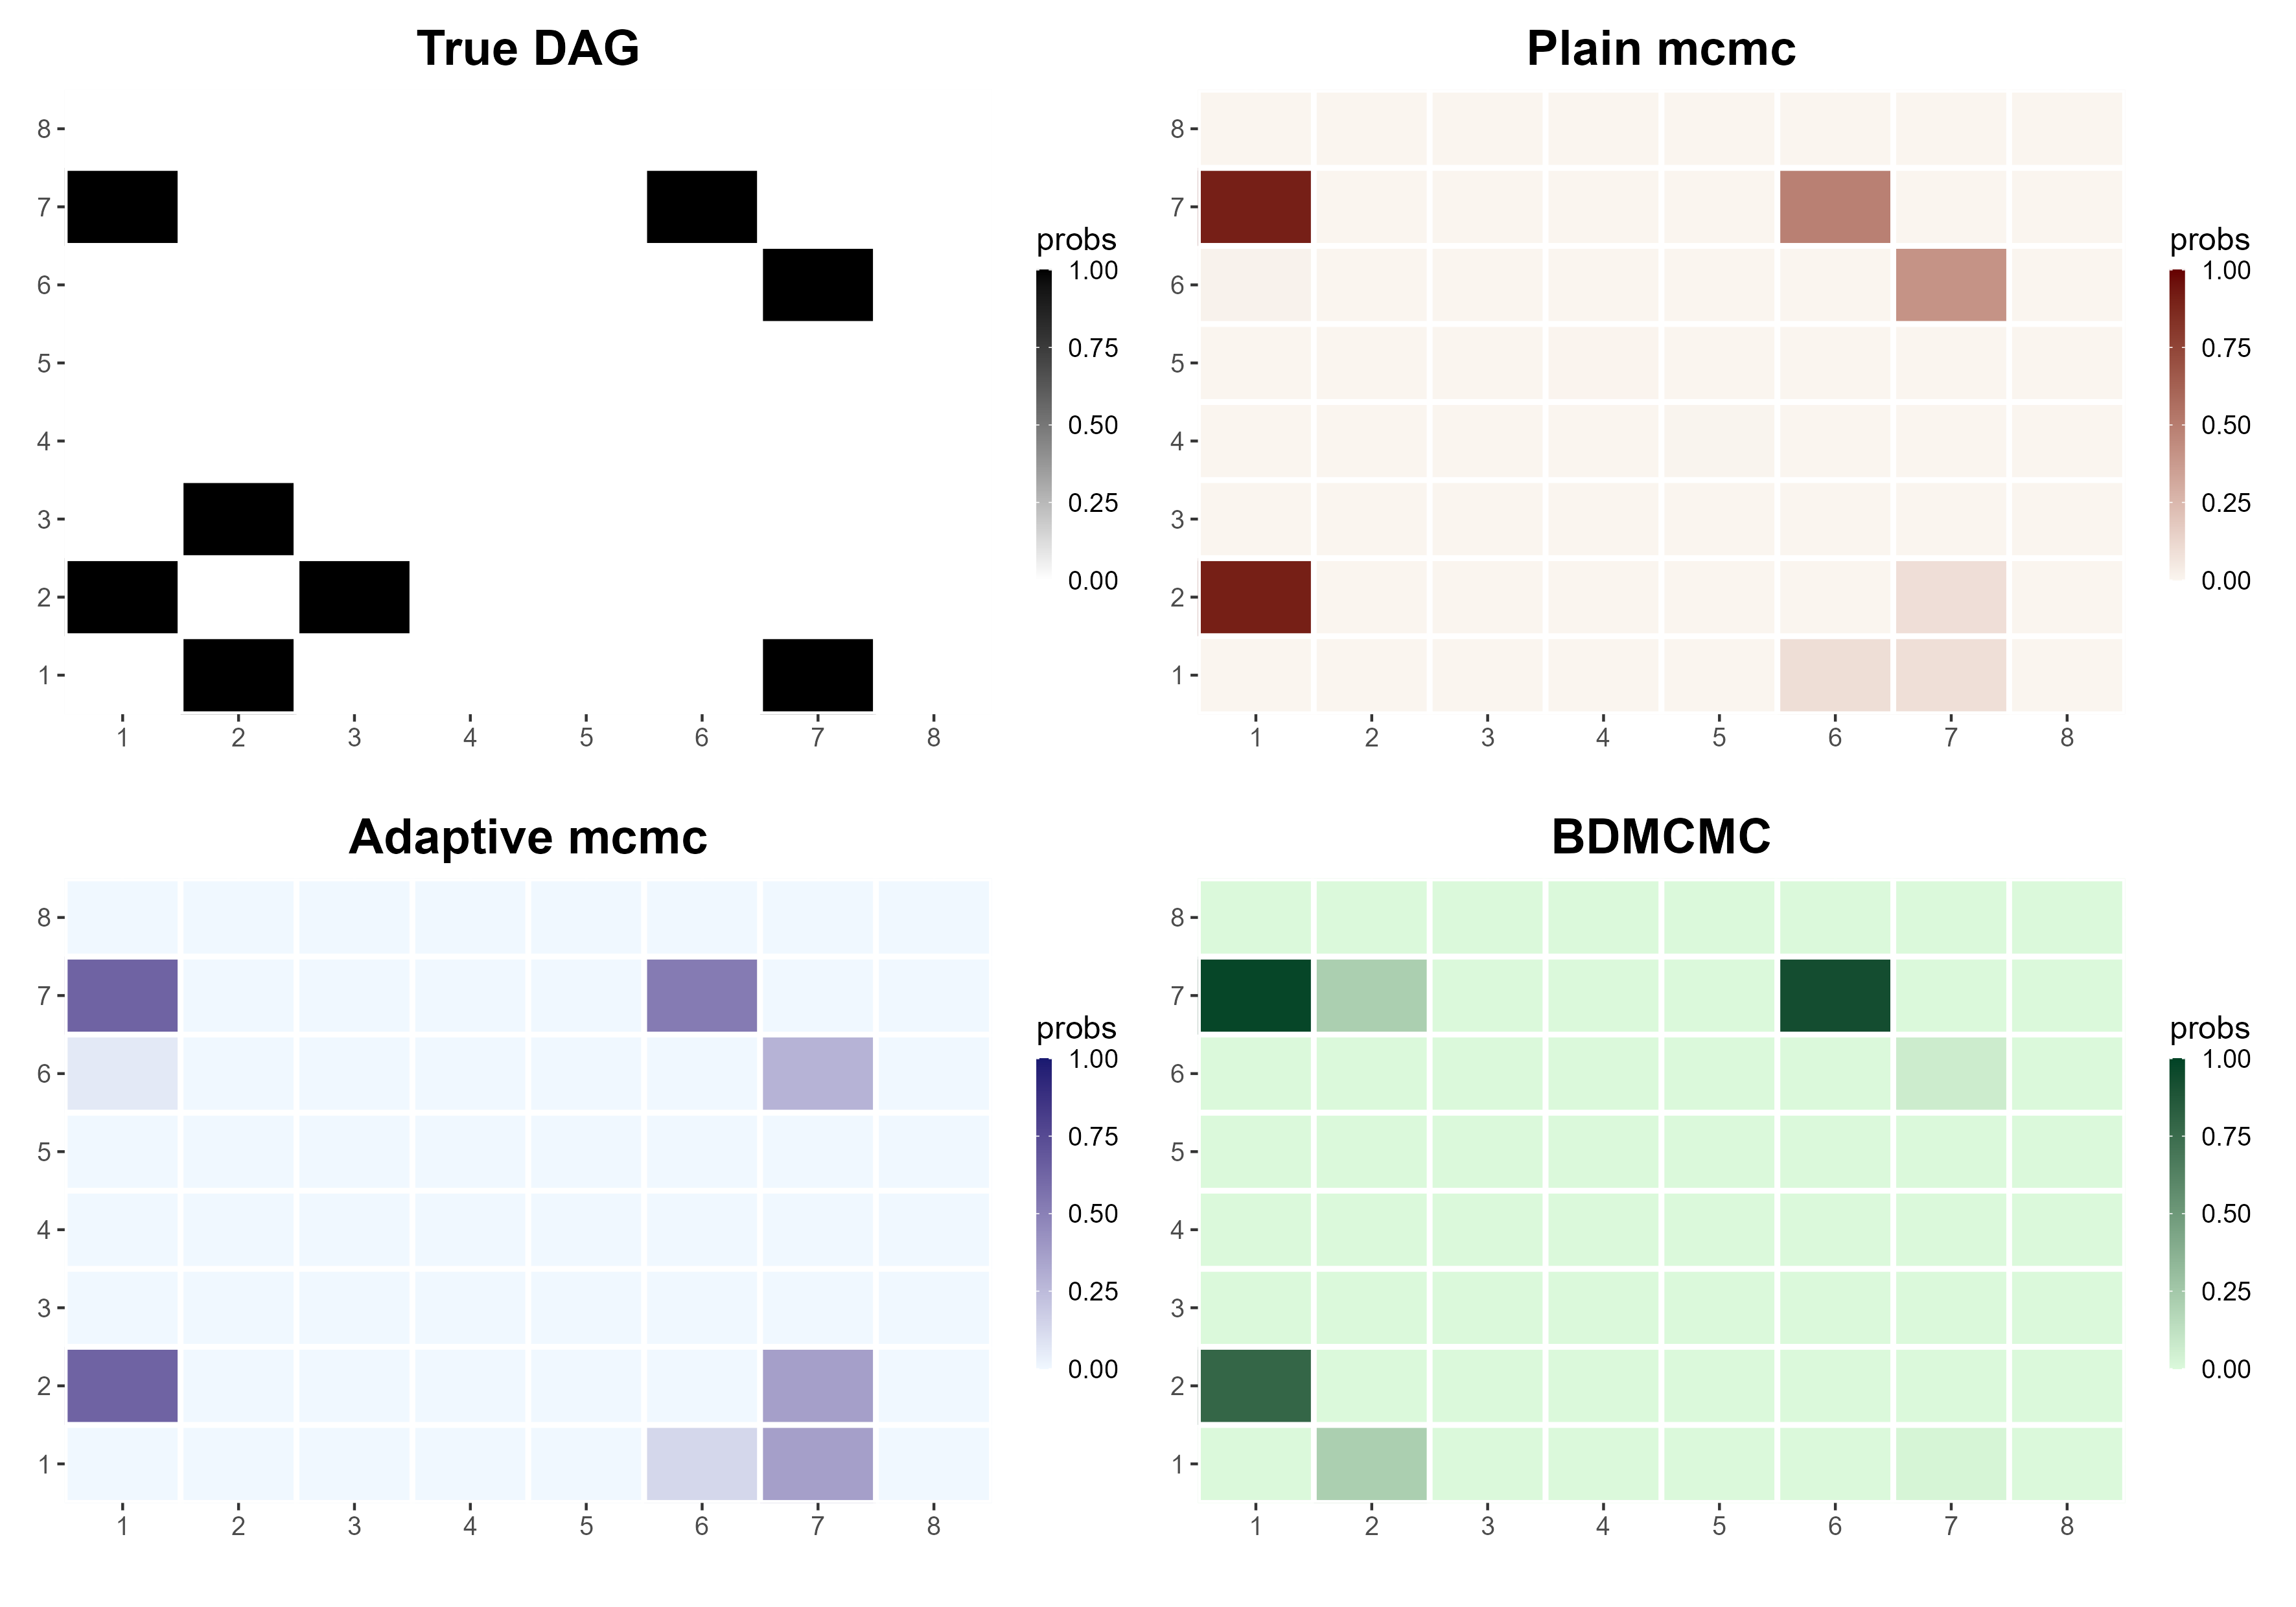
\includegraphics[width=\textwidth, height=12cm]{Figures/Overall_comparison/Random_dags/heat_dag_2_n_200.png}
				%\caption{Sample size 200}
				\label{fig:heatmaps-200}
			\end{subfigure}
			\hspace{0.35cm}  % horizontal space between figures
			% Fourth figure
			\begin{subfigure}[b]{0.45\textwidth}   
				\centering
				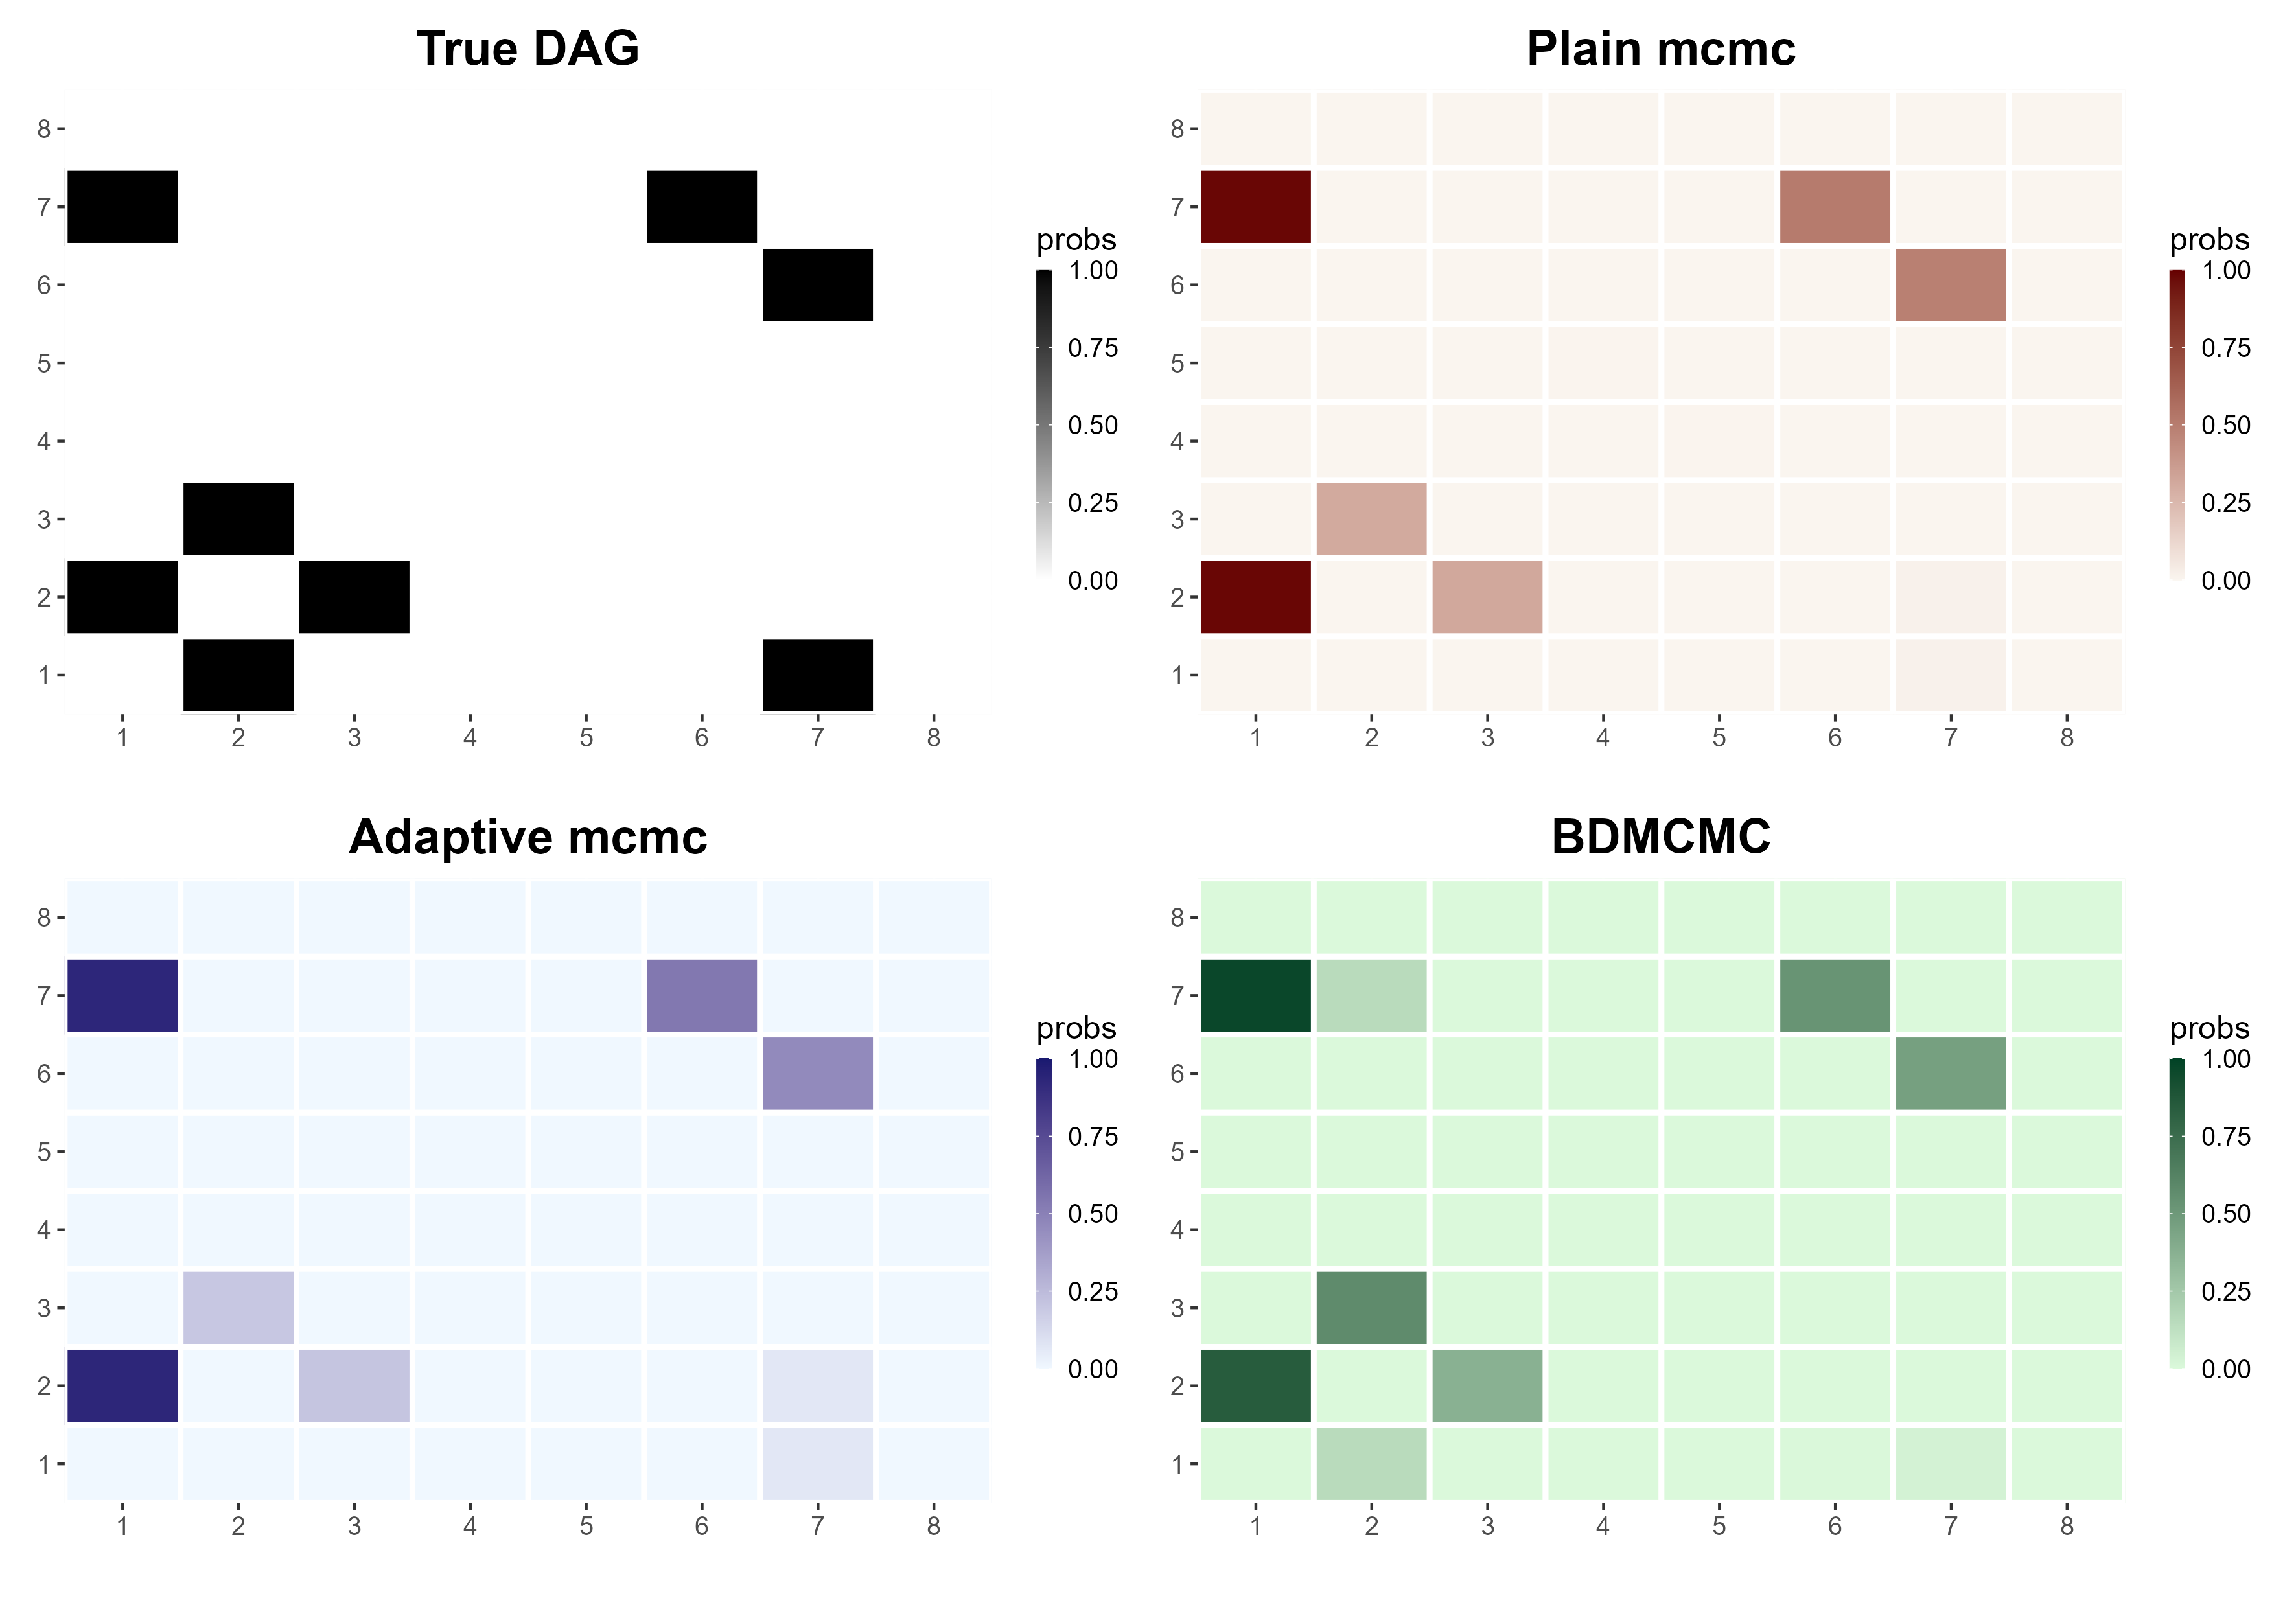
\includegraphics[width=\textwidth, height=12cm]{Figures/Overall_comparison/Random_dags/heat_dag_2_n_500.png}
				%\caption{Sample size 500}
				\label{fig:heatmaps-500}
			\end{subfigure}
			\hspace{0.35cm}
			\begin{subfigure}[b]{0.45\textwidth}   
				\centering
				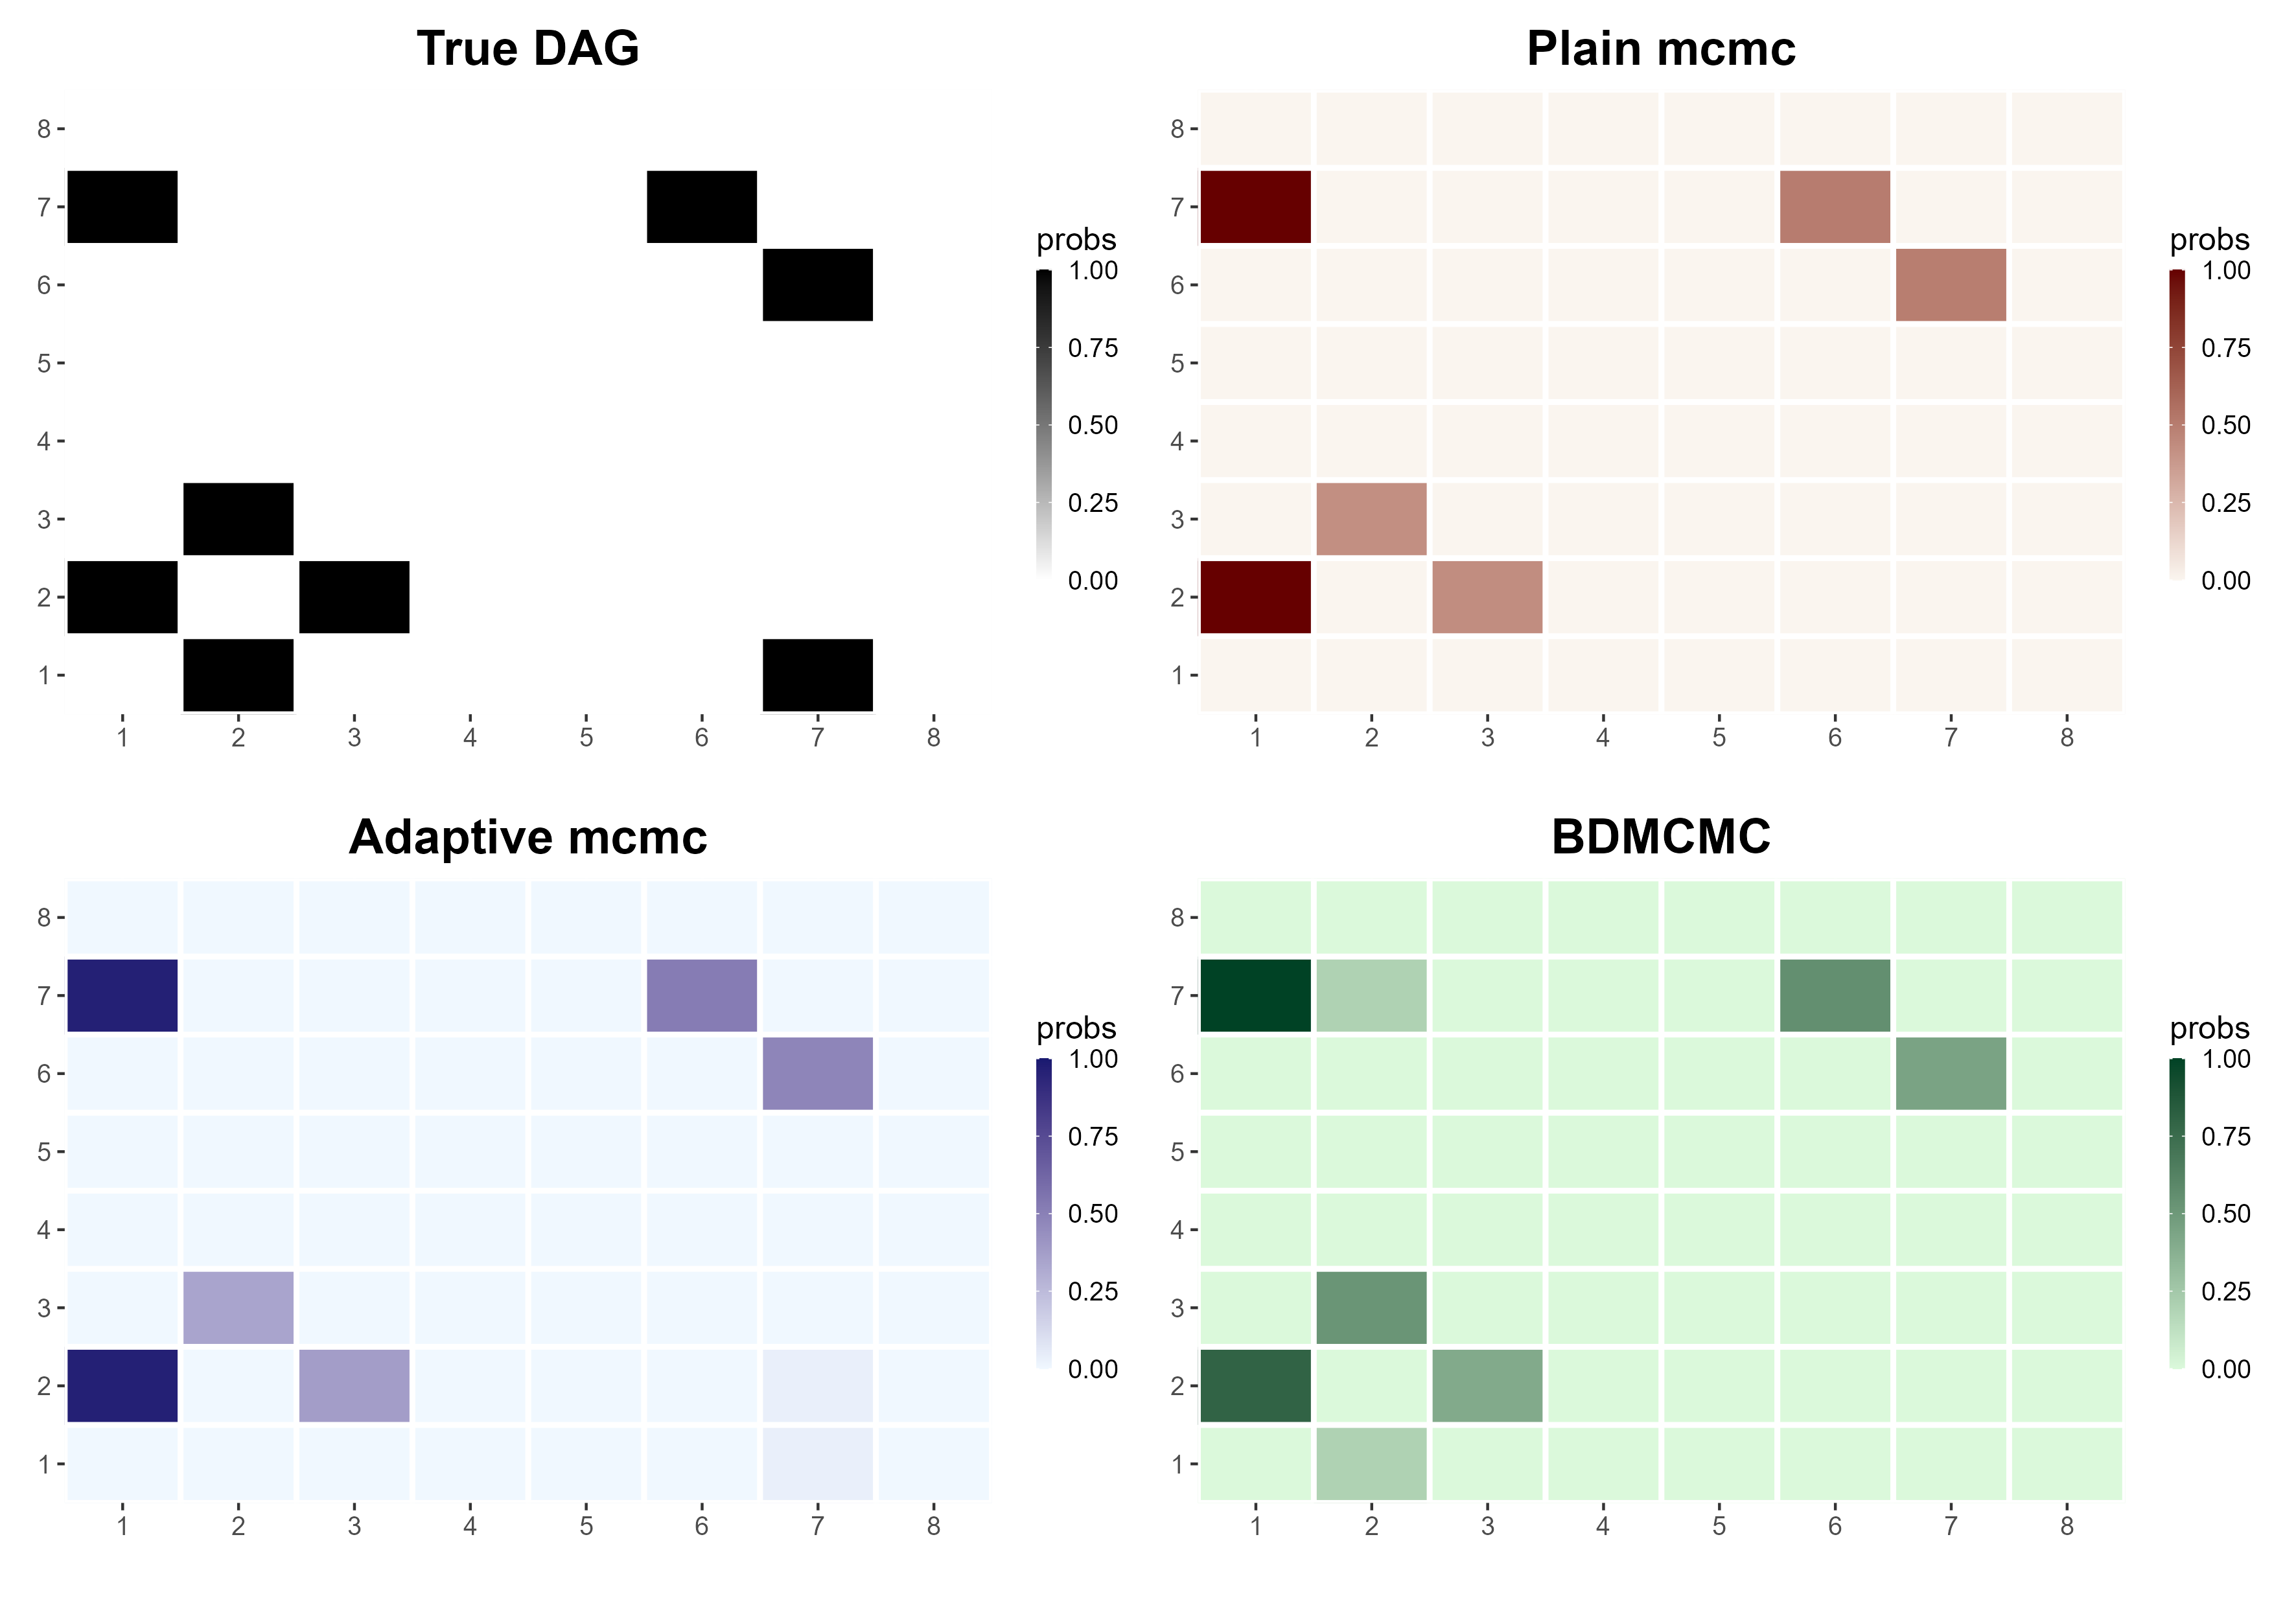
\includegraphics[width=\textwidth, height=12cm]{Figures/Overall_comparison/Random_dags/heat_dag_2_n_1000.png}
				%\caption{Sample size 1000}
				\label{fig:heatmaps-500}
			\end{subfigure}
		\end{minipage}
	}
	\caption{Performance comparison of the three algorithms for sample sizes of $n = 200$, $500$, and $1000$, using two randomly generated DAGs. The true underlying DAG used for data generation is represented in black and white.}
	\label{fig: one-two-dags}
\end{figure}

\begin{figure}[!ht]
	\centering
	\resizebox{\textwidth}{6.5cm}{  
		\begin{minipage}{\textwidth}
			\centering
			
			% First figure
			\begin{subfigure}[b]{0.45\textwidth}   
				\centering
				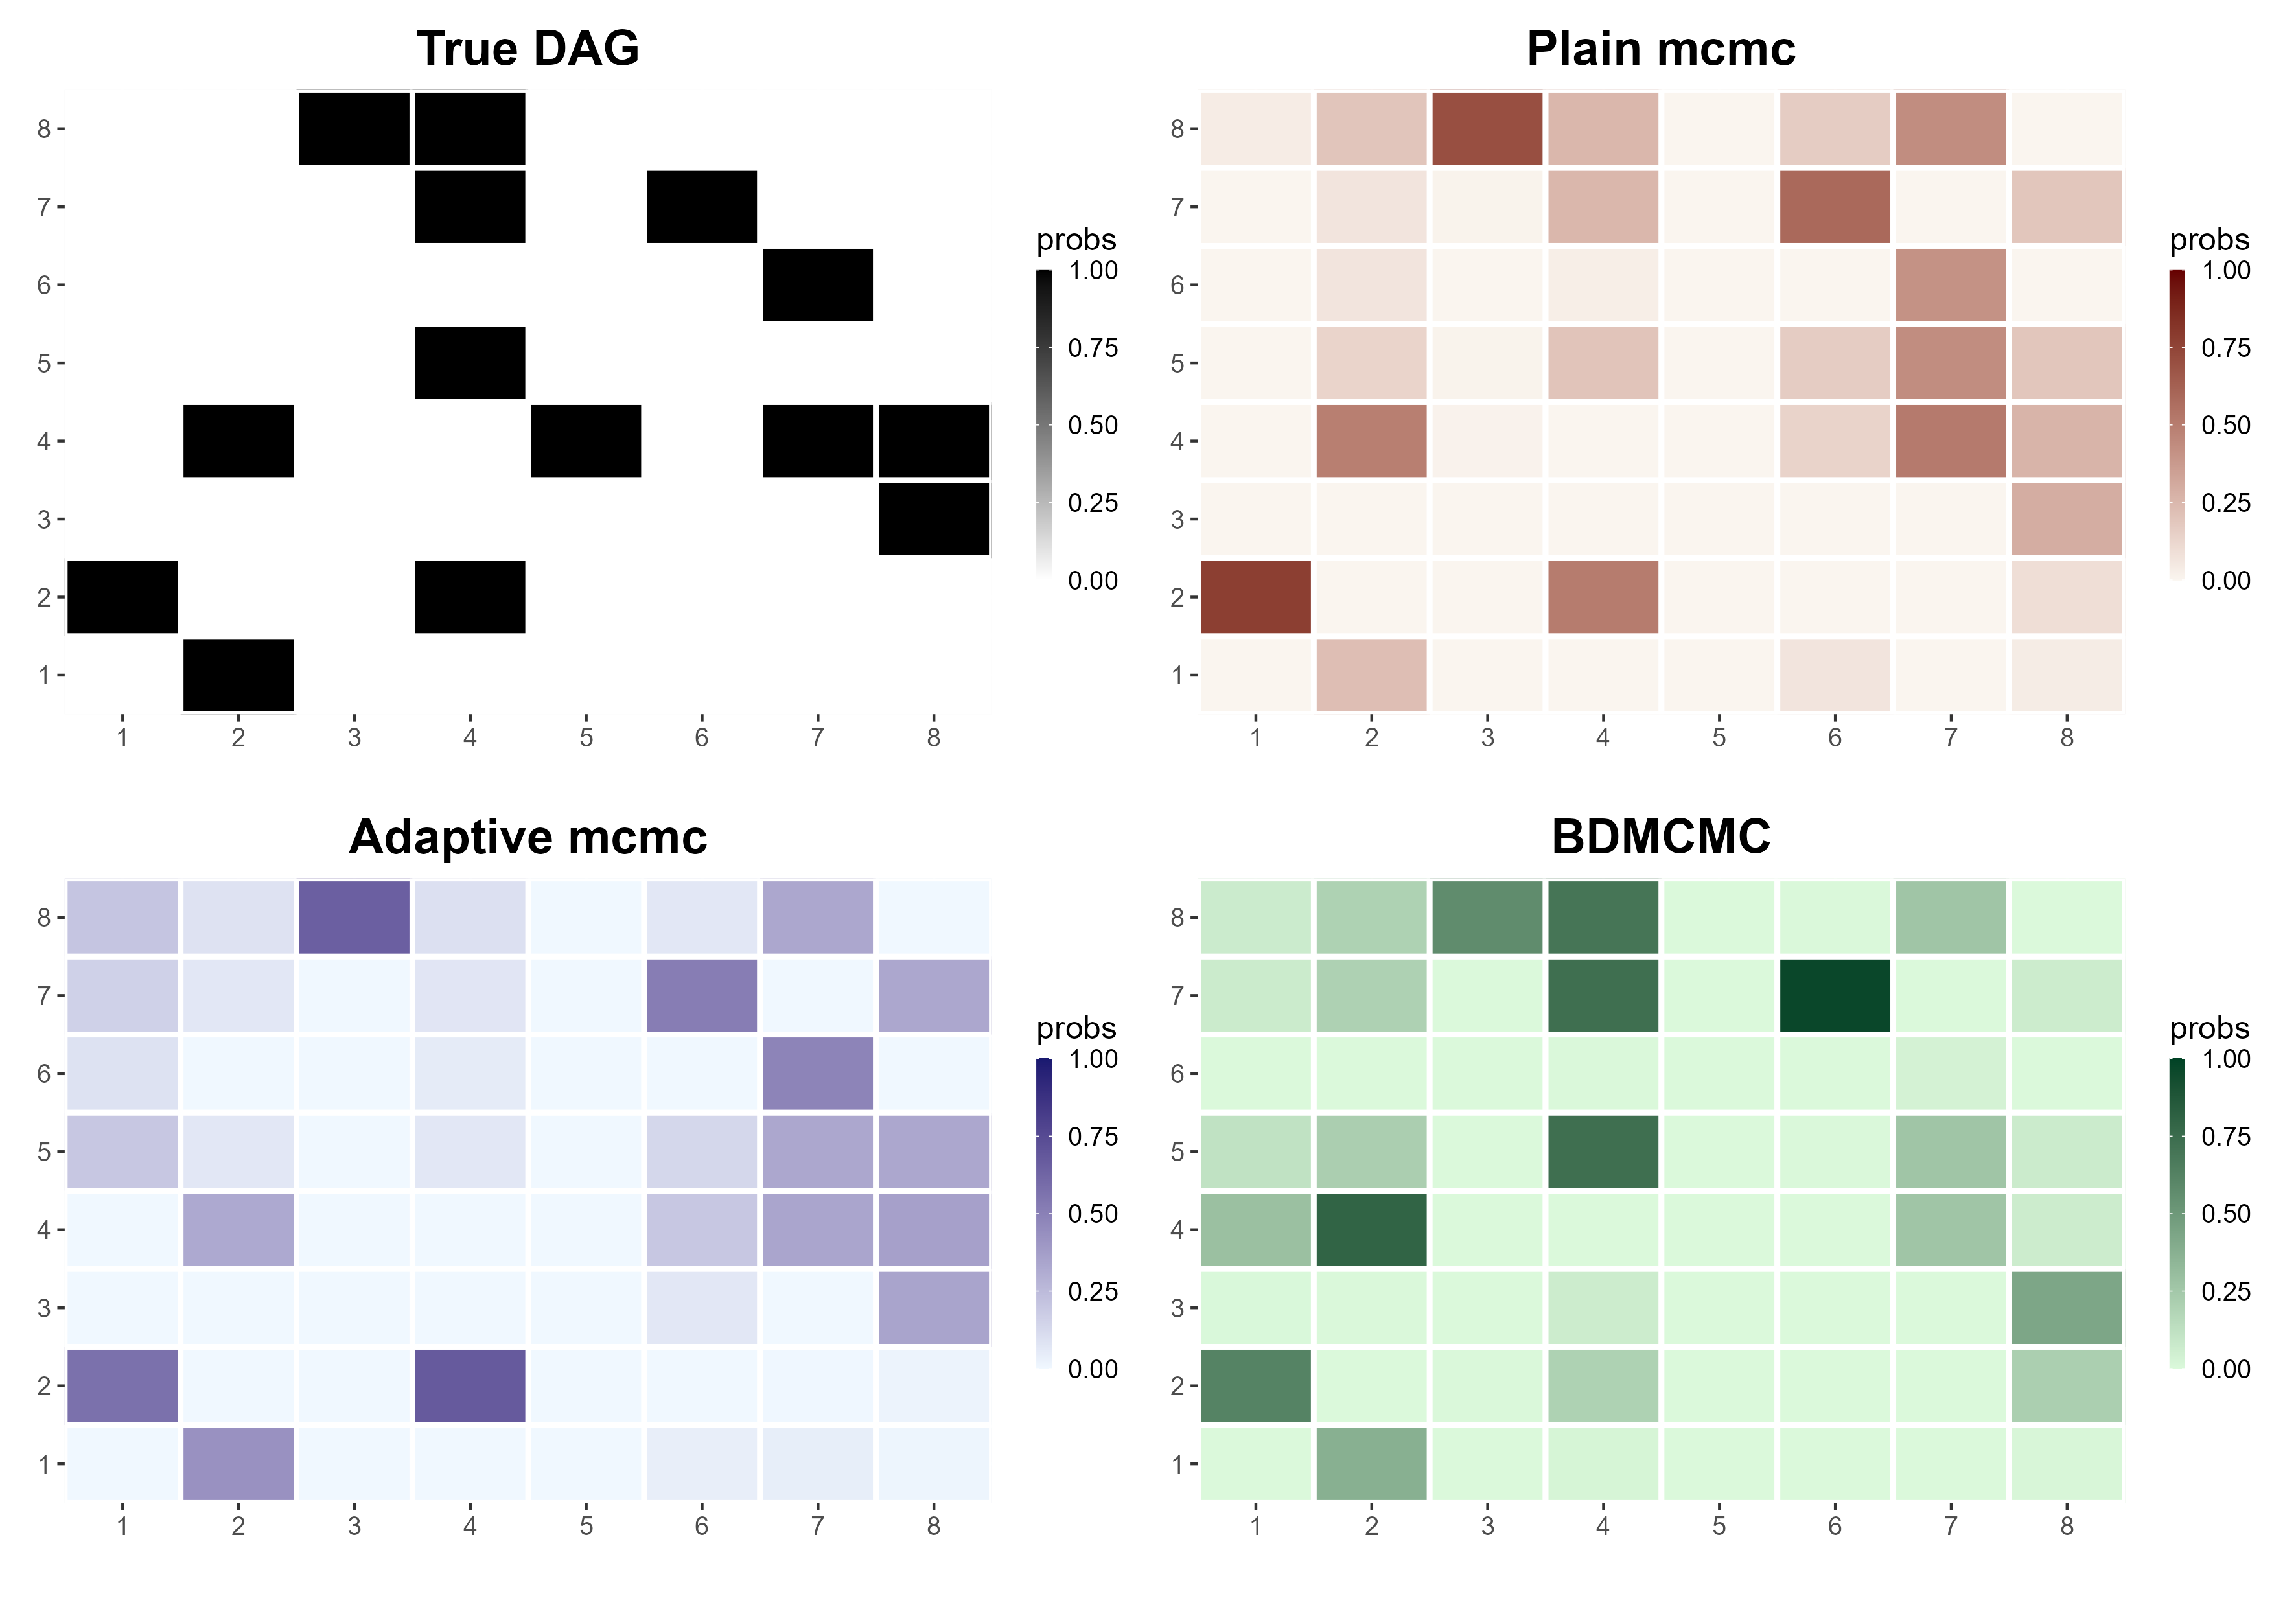
\includegraphics[width=\textwidth, height=12cm]{Figures/Overall_comparison/Random_dags/heat_dag_3_n_200.png}
				\caption{Sample size 200}
				\label{fig:heatmaps-50}
			\end{subfigure}
			\hspace{0.35cm}  % horizontal space between figures
			% Second figure
			\begin{subfigure}[b]{0.45\textwidth}   
				\centering
				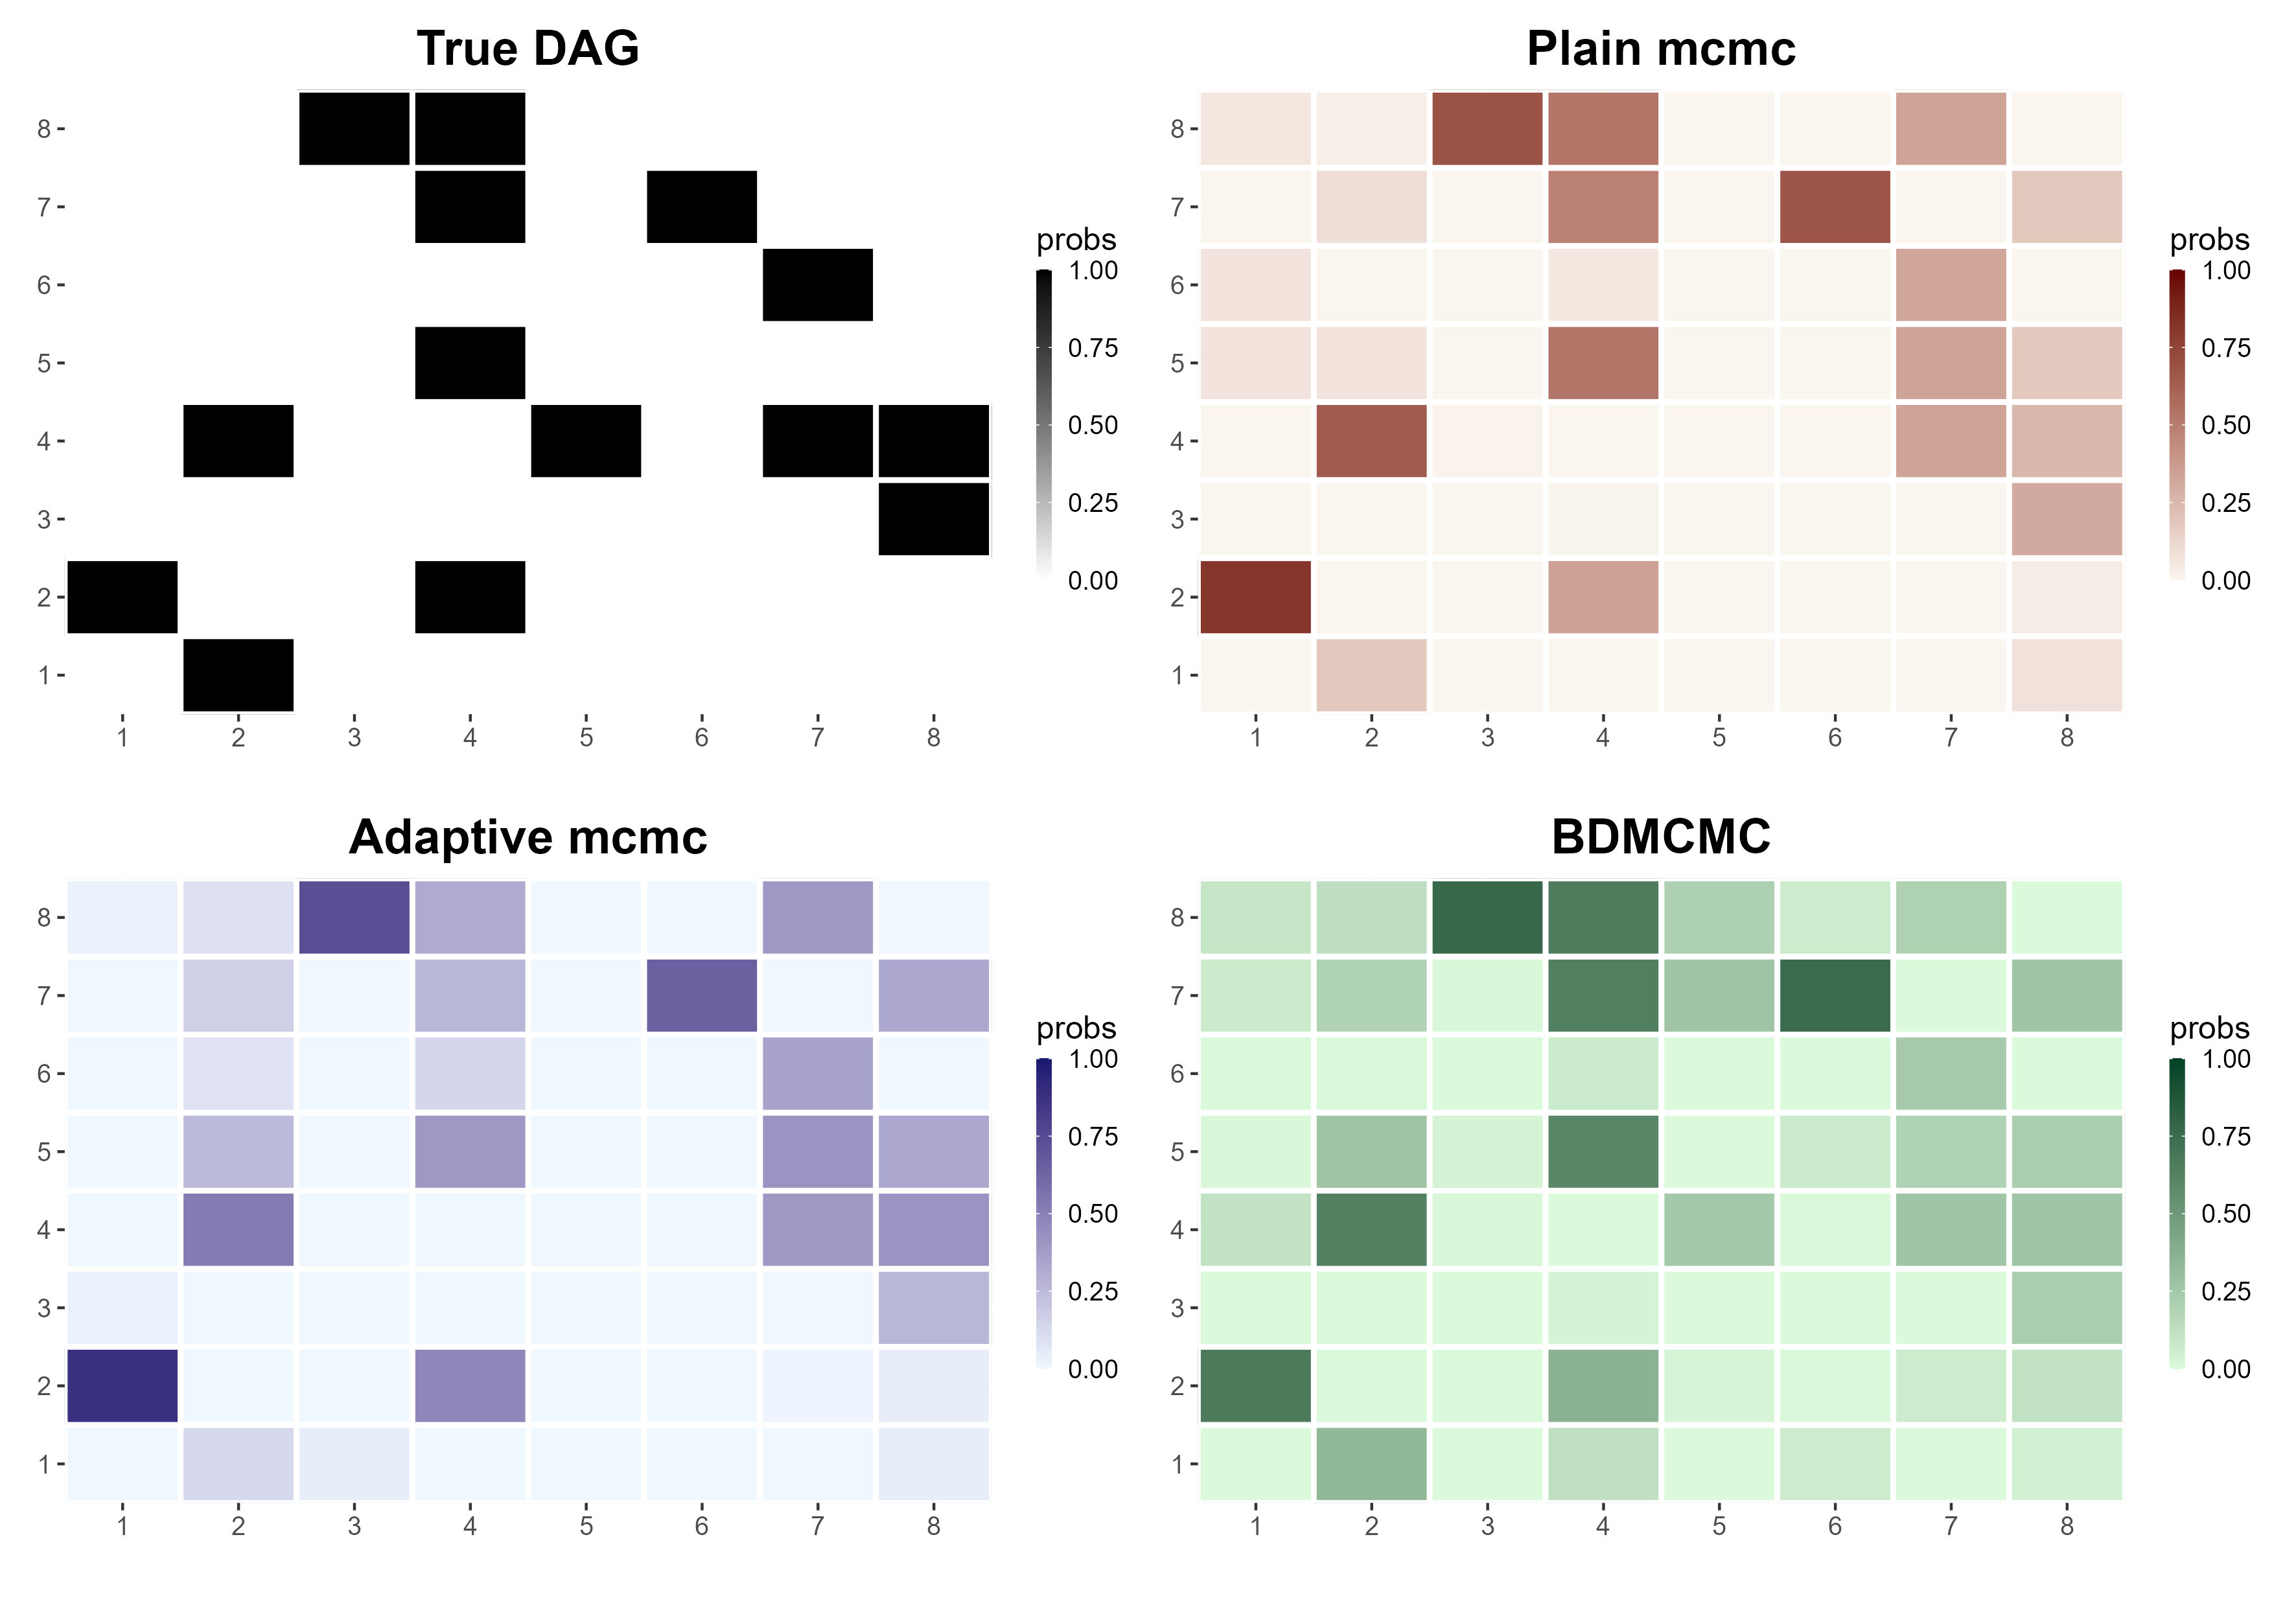
\includegraphics[width=\textwidth, height=12cm]{Figures/Overall_comparison/Random_dags/heat_dag_3_n_500.png}
				\caption{Sample size 500}
				\label{fig:heatmaps-100}
			\end{subfigure}
			\hspace{0.35cm}
			\begin{subfigure}[b]{0.45\textwidth}   
				\centering
				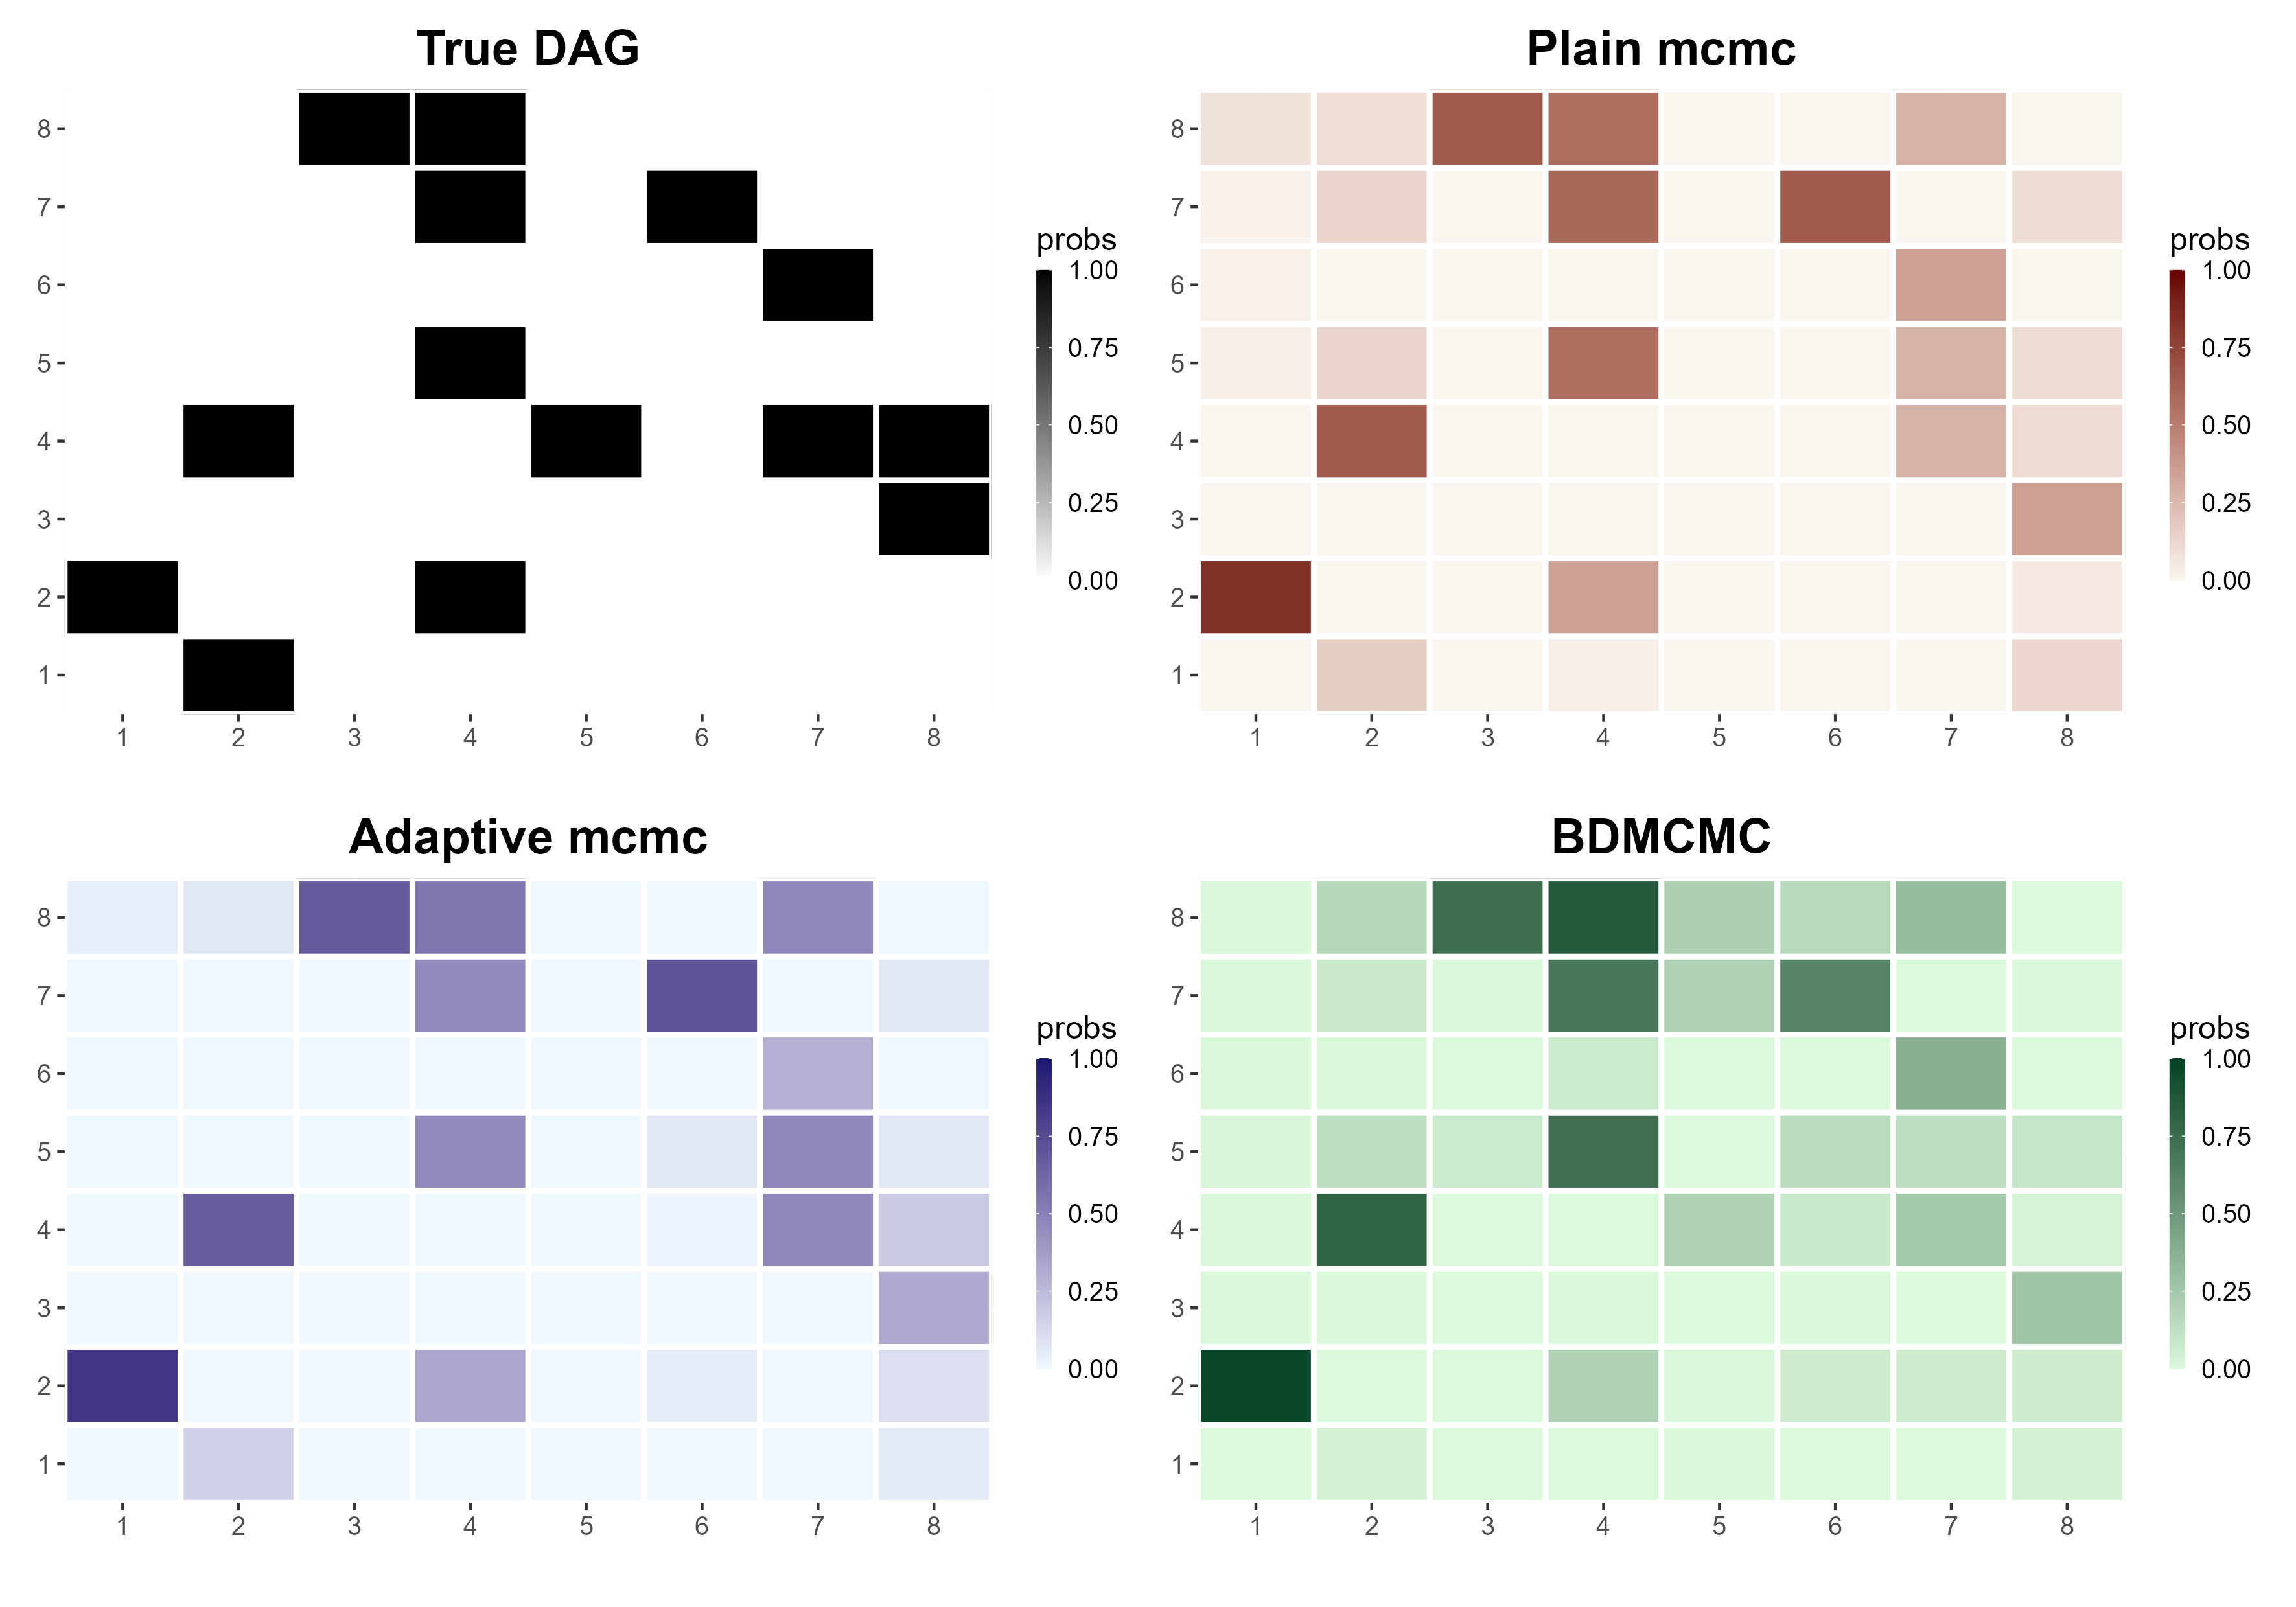
\includegraphics[width=\textwidth, height=12cm]{Figures/Overall_comparison/Random_dags/heat_dag_3_n_1000.png}
				\caption{Sample size 1000}
				\label{fig:heatmaps-100}
			\end{subfigure}
			
			\vspace{0.4cm}   %  vertical space between rows 
			
			% Third figure
			\begin{subfigure}[b]{0.45\textwidth}   
				\centering
				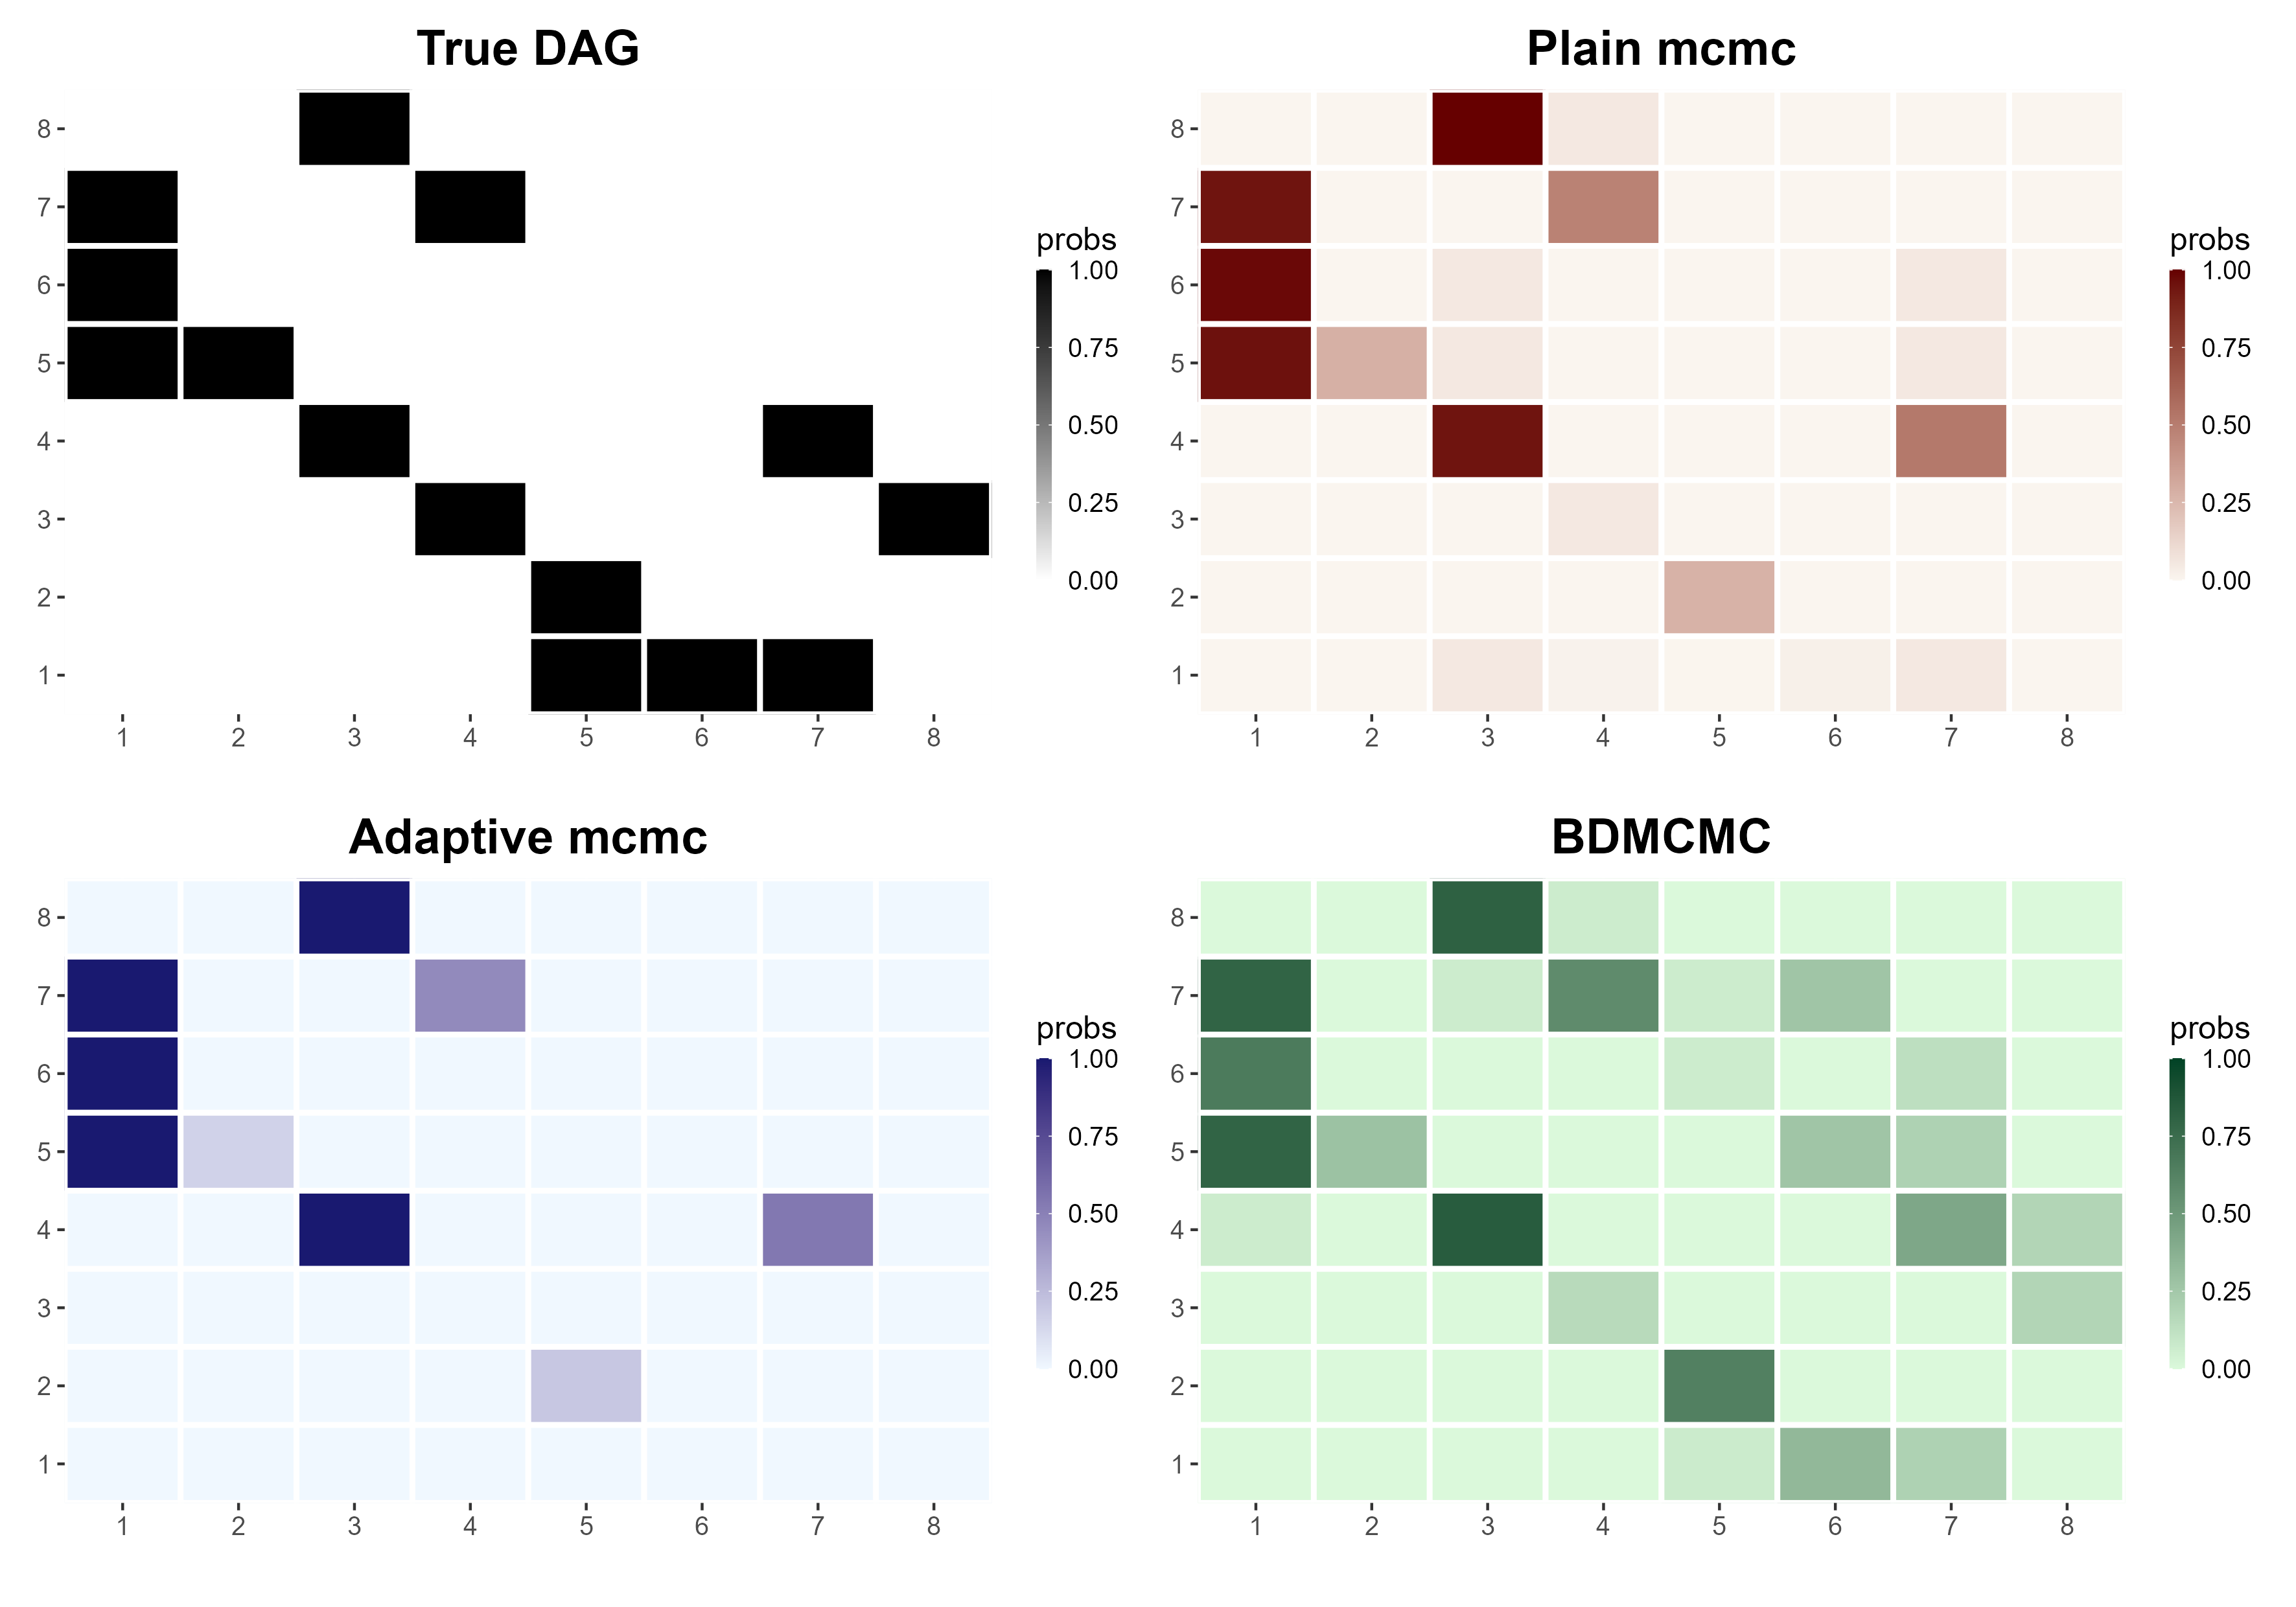
\includegraphics[width=\textwidth, height=12cm]{Figures/Overall_comparison/Random_dags/heat_dag_4_n_200.png}
				\caption{Sample size 200}
				\label{fig:heatmaps-200}
			\end{subfigure}
			\hspace{0.35cm}  % horizontal space between figures
			% Fourth figure
			\begin{subfigure}[b]{0.45\textwidth}   
				\centering
				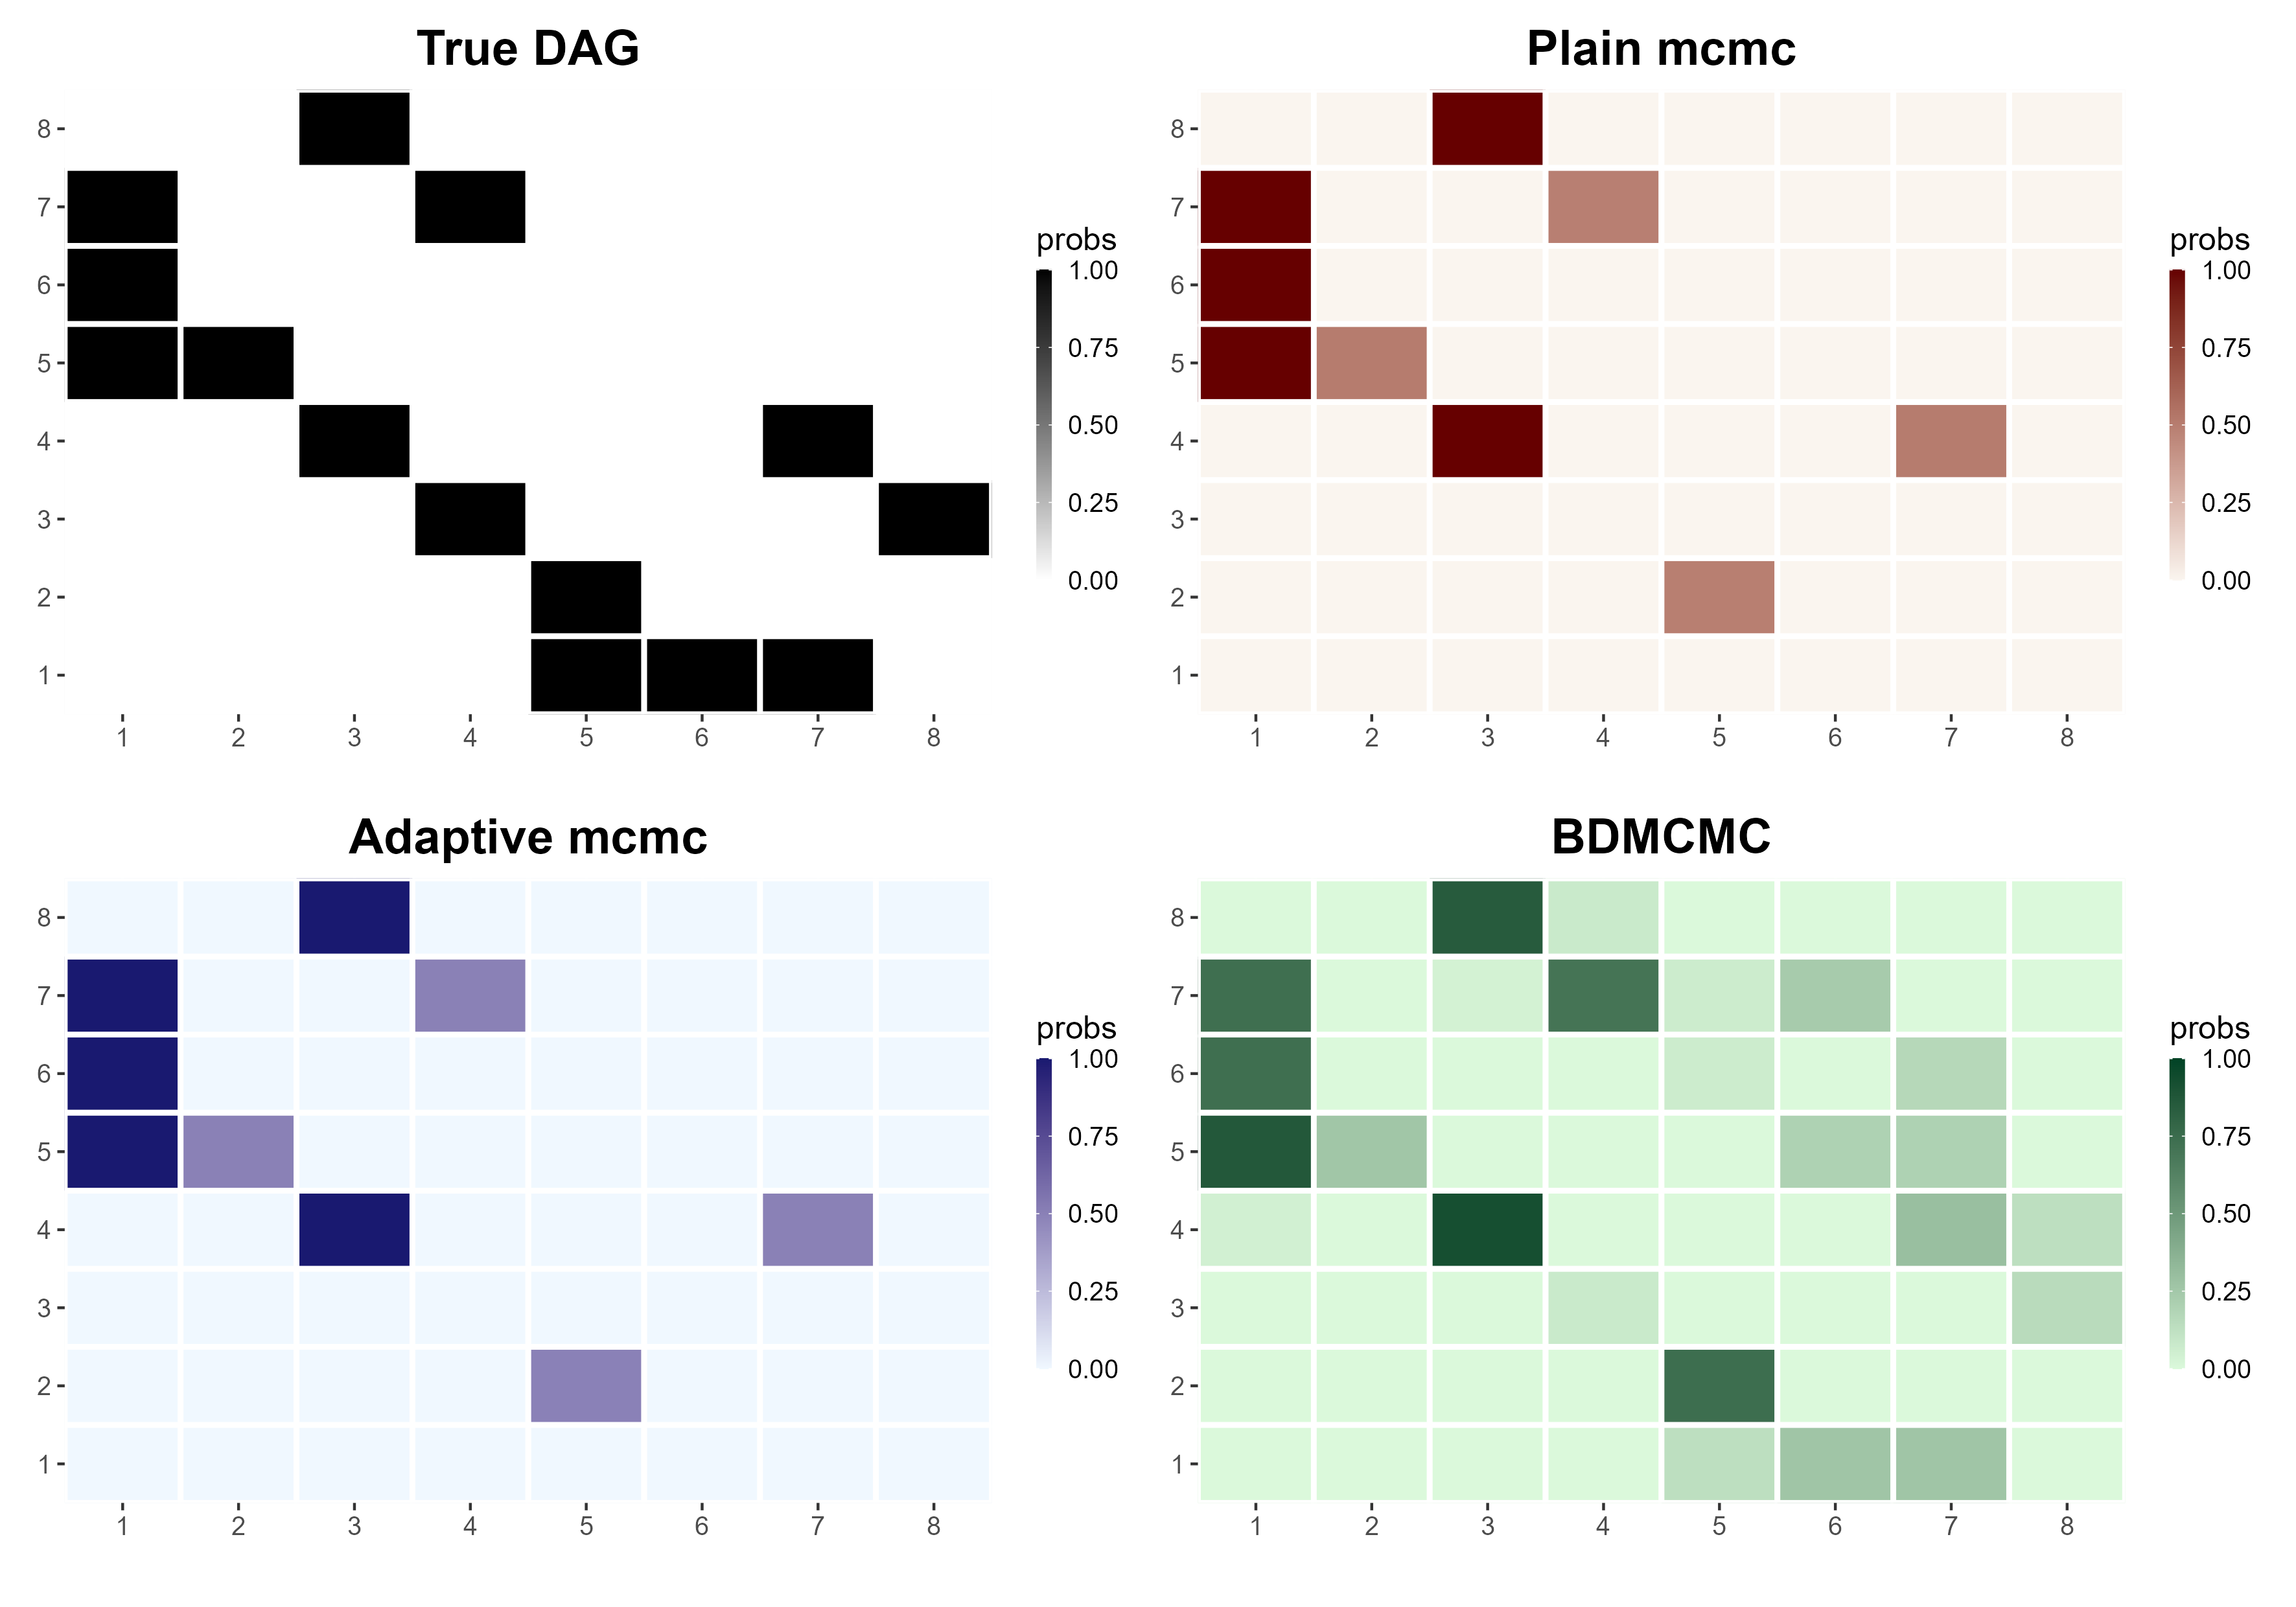
\includegraphics[width=\textwidth, height=12cm]{Figures/Overall_comparison/Random_dags/heat_dag_4_n_500.png}
				\caption{Sample size 500}
				\label{fig:heatmaps-500}
			\end{subfigure}
			\hspace{0.35cm}
			\begin{subfigure}[b]{0.45\textwidth}   
				\centering
				\includegraphics[width=\textwidth, height=12cm]{Figures/Overall_comparison/Random_dags/heat_dag_4_n_1000.png}
				\caption{Sample size 1000}
				\label{fig:heatmaps-500}
			\end{subfigure}
		\end{minipage}
	}
	\caption{Performance comparison of the three algorithms for sample sizes of $n = 200$, $500$, and $1000$, using two randomly generated DAGs. The true underlying DAG used for data generation is represented in black and white.}
	\label{fig: two-three-dags}
\end{figure}

\section{Fair Condition Benchmarking}

The comparison presented in \textit{Table} \ref{tab: shd-results} is conducted under fair conditions, ensuring that each algorithm was allocated an equal runtime of 40 seconds. During this period, intermediate results were stored by saving the corresponding R objects in an environment before the function concluded, enabling consistent and reliable evaluation across algorithms.

The Structural Hamming Distance (SHD) values reported in the table highlight the performance of the three algorithms across varying sample sizes ($n = 50, 100, 200, 500$). The results demonstrate a general trend of improvement with increasing sample size, as reflected by a decrease in SHD values. For the smallest sample size ($n = 50$), the BDMCMC algorithm exhibited the highest SHD, with a mean value of 5, indicating a lower accuracy in recovering the true graph structure. In contrast, the Adaptive and Plain Metropolis algorithms performed slightly better, with mean SHD values ranging between 4.4 and 4.6. 

As the sample size increases to 100, all algorithms exhibit a noticeable improvement in performance, with the Adaptive Metropolis (C = 0.5) scoring the highest SHD at 6.2, which indicates some instability. Conversely, both BDMCMC and Plain Metropolis achieve comparable values, around 5.5, showing their robustness at this level.

When $n = 200$, all three algorithms converge more closely, with SHD values ranging from 4 to 4.9. At this stage, the Plain metropolis appears to outperform slightly, showing the lowest SHD. 
Overall, the plain and adaptive algorithms demonstrates more stability in terms of SHD reduction as the sample size increases, particularly for larger datasets. 

\begin{table}[ht]
	\centering
	\arrayrulecolor{lightgray} % Change the line color to grey
	\begin{tabular}{
			p{3.5cm} % Adjusted column width for better display
			S[table-format=1.4, table-space-text-post = (0000)] % Align with precision and space for standard deviations
			S[table-format=1.4] % Modified to match the format of the largest value
			S[table-format=1.4] 
			S[table-format=1.4]
		}
		\toprule
		\textbf{Algorithm} & \textbf{n = 50} & \textbf{n = 100} & \textbf{n = 200} & \textbf{n = 500} \\
		\midrule
		\textit{Plain Metropolis} & {4,4 (0,5071)} & {5,5333 (1,7265)} & {4,2 (1,6562)} & {2 (1,4639)} \\
		\midrule
		\multicolumn{5}{@{}l}{\textit{Adaptive Metropolis}} \\
		C = 0.5 & {4,6 (0,5071)} & {6,2 (1,7809)} & {4,2 (1,7809)} & {2,2 (1,5213)} \\
		C = 0.7 & {4,6667 (0,488)} & {5,5333 (1,496)} & {4,0667 (1,387)} & {2,2 (1,5213)} \\
		\midrule
		\textit{Birth-Death} & {5 (0)} & {5,5333 (1,6847)} & {4,9333 (1,9809)} & {3,8667 (1,3558)} \\
		\bottomrule
	\end{tabular}
	\arrayrulecolor{black} % Revert back to black for subsequent tables
	\caption{Structural Hamming Distance: Mean values and standard errors (in parenthesis) across different algorithms and sample sizes.}
	\label{tab: shd-results}
\end{table}


\begin{figure}[h] 
	\centering
	\includegraphics[width=0.6\textwidth]{Figures/Overall_comparison/shd_timing.png}
	\caption{Structural Hamming Distance across varying sample sizes, given a fixed maximum running time.}
	\label{fig:box-shd-time}
\end{figure}

\textit{Figure} \ref{fig:box-shd-final} provides a comparison of the algorithms' Structural Hamming Distance performance across varying sample sizes, reflecting their ability to recover the correct graph structure. The boxplots are constructed using 15 replicates for each sample size, ensuring that the results are not biased by random fluctuations and offer a comprehensive view of the algorithms' behavior.

The results reveal several key patterns:

\begin{enumerate}
	\item For a sample size of $n = 50$, the three Metropolis-based algorithms (Plain Metropolis and Adaptive with $C = 0.5$ and $C = 0.7$) perform similarly, with no substantial differences in their SHD distributions. This suggests that at such a small sample size, all three struggle equally to capture the underlying structure due to insufficient data.
	\item At $n = 100$, a divergence in performance is observed. The Adaptive Metropolis with $C = 0.7$ shows clear improvements over the Plain Metropolis, achieving a lower SHD up to 30,000 iterations. Conversely, the Adaptive algorithm with $C = 0.5$ struggles the most, yielding the highest SHD across all iterations, indicating a weaker adaptation to the data.
	\item For $n = 200$, both Adaptive Metropolis algorithms ($C = 0.5$ and $C = 0.7$) consistently outperform the Plain Metropolis, which suggests that incorporating adaptivity with these parameter settings helps in capturing the correct graph structure more effectively as the sample size increases.
	\item With $n = 500$, the differences between the three algorithms become minimal in the early stages of the iterations. However, beyond 48,000 iterations, the Plain Metropolis begins to outperform both Adaptive versions. This phenomenon can be attributed to the Plain Metropolis’s unrestricted exploration of the model space, allowing it to eventually settle into better configurations when given a sufficient number of iterations.
\end{enumerate}

The Birth-Death MCMC algorithm requires a separate interpretation due to its fundamentally different nature and stopping criterion. Unlike the Metropolis algorithms, it is guided by a score, namely the waiting time.
In \textit{Figure} \ref{fig:trace-shd-BD}, the traceplots of SHD for various sample sizes across different runs reveal a distinct pattern. The Birth-Death algorithm does not automatically stop upon reaching a local minimum of SHD. Instead, it investigates the neighborhood of the current solution through a series of local moves, which is evident from the traceplots. This ability to navigate the model space is advantageous, as it allows the algorithm to avoid early stopping and potentially escape suboptimal solutions.

The traceplots further illustrate that the Birth-Death algorithm effectively reduces SHD in just a few iterations, demonstrating its capability to rapidly capture essential features of the underlying graph structure. Additionally, the fact that the algorithm occasionally allows SHD to increase before converging indicates a deliberate exploration strategy, which helps it to evaluate the stability and robustness of its selected configurations. Thus, the Birth-Death MCMC seems to provide a nuanced balance between global and local search strategies, making it particularly suitable for complex model spaces.

\begin{figure}[!ht]
	\centering
	\begin{minipage}{\textwidth}
		\centering
		
		% First figure
		\begin{subfigure}[b]{0.45\textwidth}   
			\centering
			\includegraphics[width=\textwidth, height=6cm]{Figures/Overall_comparison/Boxplot_shd_iters_plain.png}
			\caption{Plain metropolis}
			\label{fig:box-plain}
		\end{subfigure}
		\hspace{0.35cm}  % horizontal space between figures
		% Second figure
		\begin{subfigure}[b]{0.45\textwidth}   
			\centering
			\includegraphics[width=\textwidth, height=6cm]{Figures/Overall_comparison/Boxplot_shd_iters_c07.png}
			\caption{Adaptive, C = 0.7}
			\label{fig:box-c07}
		\end{subfigure}
		
		\vspace{0.4cm}   %  vertical space between rows 
		
		% Third figure
		\begin{subfigure}[b]{0.45\textwidth}   
			\centering
			\includegraphics[width=\textwidth, height=6cm]{Figures/Overall_comparison/Boxplot_shd_iters_c05.png}
			\caption{Adaptive, C = 0.5}
			\label{fig:box-c05}
		\end{subfigure}
	\end{minipage}
	
	\caption{Boxplots illustrating the Structural Hamming Distance across iterations and algorithms (Plain MCMC and two variations of the Adaptive algorithm), based on 15 replicates.}
	\label{fig:box-shd-final}
\end{figure}

\begin{figure}[h] 
	\centering
	\includegraphics[width=0.8\textwidth]{Figures/Overall_comparison/trace_shd_iters_BD.png}
	\caption{Traceplot of Structural Hamming Distance for the Birth-Death model across iterations, based on 10 replicates for each sample size.}
	\label{fig:trace-shd-BD}
\end{figure}

\section{Final Observations and Comments}

Overall, the Birth-Death MCMC algorithm shows potential due to its informed criterion, which evaluates the goodness-of-fit of the DAG through a score-based mechanism. This approach allows the algorithm to actively search for configurations that best represent the underlying structure. Nevertheless, the algorithm's performance can be further refined. One concern is the larger variability of the SHD observed in Birth-Death MCMC compared to the Metropolis-based approaches, which consistently provide more stable estimates, as seen in the boxplots and earlier diagnostic evaluations.

One of the notable drawbacks of traditional MCMC methods is the computational burden associated with storing and manipulating the resulting matrices. Due to the high-dimensional nature of DAGs, a large number of matrices must be retained across iterations, which can become impractical. A commonly employed strategy to alleviate this issue is to encode the adjacency matrices as binary strings. While this reduces memory requirements, reconstructing the DAGs from these strings to analyze the algorithm's behavior still incurs significant computational overhead. In contrast, the Birth-Death MCMC generates fewer sampled configurations and focuses on maximizing a well-defined score, making it less cumbersome to handle computationally and more straightforward to analyze.

Another advantage of the Birth-Death algorithm is its capacity to explore a wider range of configurations through global moves, whereas MCMC, especially the Adaptive variants, can become trapped in local minima due to their reliance on local transitions. The Birth-Death mechanism, by evaluating the waiting time, maintains a balance between local and global search, allowing it to navigate the model space more comprehensively. Its scoring mechanism and stopping criterion provide it with more flexibility compared to purely local Metropolis-based updates.

Given its exhaustive exploration, Birth-Death can serve as an effective initial exploratory tool. It has the potential to guide the search for a better configuration space, providing initial candidate models that Metropolis algorithms can refine. Thus, it can be used in tandem with other MCMC methods, suggesting good starting points for subsequent optimization and potentially reducing the risk of premature convergence in Metropolis-based algorithms.

Lastly, the parameter sampling for both MCMC and Birth-Death is facilitated by the availability of full conditional distributions in closed form, specifically the DAG-Wishart distribution. This allows for efficient sampling of parameters, making the entire process faster and less prone to computational bottlenecks. With further improvements, such as enhanced score functions or hybrid strategies combining Birth-Death with adaptive mechanisms, the Birth-Death MCMC could become a robust alternative for scenarios where global structure learning is crucial.

\chapter{Case Study: Application of Bayesian Networks in Biomedical Research}

\section{Overview of Abatacept’s Impact on the CD28 Pathway in Early Systemic Sclerosis}

Systemic sclerosis (SSc) is a complex autoimmune disease characterized by skin thickening and fibrosis, with impacts that vary widely among patients depending on specific genetic and molecular pathways. In recent years, precision medicine has begun to transform the approach to treating such conditions, focusing on identifying patient subgroups most likely to benefit from specific therapies. A central concept in precision medicine is the molecular pathway, which refers to a series of interactions among molecules within a cell that lead to a specific function or change, such as cell signaling, gene expression, or immune activation. By understanding these pathways, scientists can pinpoint disease mechanisms and potential therapeutic targets. One of the key molecular pathways implicated in SSc, especially in its early and diffuse form (dcSSc), is the CD28 costimulation pathway. This pathway plays a critical role in immune response regulation, particularly in inflammation and immune cell activation, and may therefore represent a targetable mechanism for therapeutic intervention.

Abatacept, an immunomodulatory drug, has shown promise in modulating the CD28 pathway in patients with early dcSSc. It is thought to work by altering immune cell activity, potentially benefiting patients with heightened inflammatory responses. A clinical trial in 2022 investigated this by examining 84 dcSSc patients, randomizing them to receive either abatacept or a placebo. Changes in clinical severity, measured by the modified Rodnan skin score (mRSS), were assessed over 12 months, with RNA-seq data from paired skin biopsies used to explore the impact of treatment on gene expression profiles. The findings suggested that patients in the inflammatory gene expression subset responded most strongly to abatacept, showing significant reductions in skin fibrosis and movement toward a “normal-like” gene expression pattern (\citet{mehta2022machine}).

This study forms the foundation for the present analysis, where the goal is to better understand the gene dependencies and network relationships within the CD28 pathway in patients treated with abatacept compared to those on placebo. This study aims to estimate the posterior probabilities of gene interaction presence in directed acyclic graphs within the CD28 pathway.
It is hypothesized that treatment with abatacept may alter the dependencies within the CD28 pathway, potentially increasing certain dependencies as a result of the drug’s modulation of immune responses. Such changes could reflect a shift in network connectivity, where abatacept drives specific gene interactions that might contribute to its therapeutic effects.

\section{Study Design and Statistical Assumptions}

Dependencies within the CD28 pathway are analyzed by modeling dependencies among gene expression variables in the context of systemic sclerosis treatment. The approach assumes that the conditional independencies inherent in the multivariate distribution of observational data are encoded within a Directed Acyclic Graph, where nodes represent variables and directed edges indicate dependencies, as dictated by the Markov property associated with the graph (\citet{friedman2004inferring}). Each DAG structure implies a specific factorization of the joint distribution over the data, reflecting underlying conditional independencies. However, a DAG model is typically not uniquely identifiable from observational data alone. Instead, what can be reliably estimated is its Markov equivalence class—a set of DAGs that encode the same conditional independencies. 

To address this uncertainty, a Bayesian framework is employed to model the equivalence class. This framework uses priors informed by a Gaussian distribution consistent with the DAG factorization, with a modified Cholesky decomposition of precision matrices used to specify priors over the entire class of DAGs. In particular, it holds that:

$$
\mathbf{L}^T \mathbf{x} = \epsilon
$$

A Bernoulli-beta prior on the adjacency matrix of the skeleton integrates assumptions on sparsity, which is especially pertinent in gene regulatory contexts. The prior is encoded as follows:

\begin{align*}
	\mathcal{D}_j | \pi &\sim Ber(\pi), \quad j = 1, \ldots, \frac{q(q-1)}{2} \\
	\pi &\sim Beta(a, b)
\end{align*}

In addition, the DAG-Wishart properties result in the prior of the node parameters $\{(\mathbf{D}_{jj}, \mathbf{L}_{\prec j]})\}$ being a priori independent with distribution:

\begin{equation} 
	\begin{split}
		\mathbf{D}_{jj} | \mathcal{D} \sim I-Ga  \biggl( \frac{1}{2} a^{\mathcal{D}}_j, \frac{1}{2}\mathbf{U}_{jj | pa_{\mathcal{D}} (j)} \biggr ) \\
		\mathbf{L}_{\prec j]} | \mathbf{D}_{jj}, \mathcal{D} \sim N_{pa_{\mathcal{D}} (j)} \Bigl(- \mathbf{U}^{-1}_{\prec j \succ} \mathbf{U}_{\prec j ]}, \mathbf{D}_{jj}\mathbf{U}^{-1}_{\prec j \succ} \Bigr )
	\end{split}
\end{equation}

The parameter $\alpha^{\mathcal{D}}$ is chosen to take the value $a + \left| pa_{\mathcal{D}} (j) - q + 1 \right| \ (a > q - 1)$ in order to assume compatibility among prior distributions for Markov equivalent DAGs.

In this analysis, faithfulness is assumed, meaning that the conditional independencies present in the data can be accurately represented by a multivariate normal distribution. Under this assumption, conditional independencies among variables can be identified using techniques like d-separation or the moral graph approach (\citet{lauritzen1989graphical}). For a joint distribution that is multivariate Gaussian, these independencies impose certain structural constraints on the covariance matrix of the variables $X_1,\dots, X_q$.

\section{Descriptive and Inferential Statistical Analysis}

In \textit{Table} \ref{table:count}, the raw counts for both placebo and Abatacept-treated patients are displayed, with counts provided at Baseline (before treatment initiation) and at 3 and 6 months post-treatment. The distribution of patients appears balanced overall, with the placebo group containing only six more patients than the treatment group.

\begin{table}[!ht]
	\centering
	\begin{tabular}{|l|l|c|c}
		\hline
		\textbf{Timing} & \textbf{Placebo} & \textbf{Abatacept} \\ \hline
		Baseline & 43 & 43 \\ 
		Month-3 & 38 & 34 \\ 
		Month-6 & 40 & 35 \\ \hline
		\textbf{Total} & 118 & 112 \\ \hline
	\end{tabular}
	\caption{counts}
	\label{table:count}
\end{table}

\textit{Table} \ref{table:detailed-counts} provides a detailed breakdown of patients by subtype: normal-like, inflammatory, and fibroproliferative. Patients in the inflammatory subset exhibit heightened immune and fibrotic activity, while those in the fibroproliferative subset display increased fibrotic, immune, and cell-cycle-related processes. The normal-like subset includes patients whose gene expression patterns more closely resemble those of healthy controls. This classification enables a closer examination of treatment effects across distinct biological profiles within each group.

\begin{table}[ht]
	\centering
	\begin{tabular}{
			p{2.5cm}
			S[round-mode = places, round-precision = 0]
			S[round-mode = places, round-precision = 0]
		}
		\toprule
		& {Placebo} & {Abatacept} \\
		\midrule
		\multicolumn{3}{@{}l}{\textit{Baseline}} \\
		Normal like & 19 & 15 \\
		Inflammatory & 14 & 20 \\
		Proliferative & 10 & 8 \\
		\midrule
		\multicolumn{3}{@{}l}{\textit{After 3 months}} \\
		Normal like & 15 & 13 \\
		Inflammatory & 13 & 13 \\
		Proliferative & 10 & 6 \\
		\midrule
		\multicolumn{3}{@{}l}{\textit{After 6 months}} \\
		Normal like  & 17 & 12 \\
		Inflammatory & 13 & 15 \\
		Proliferative & 10 & 8 \\
		\bottomrule
	\end{tabular}
	\caption{Detailed counts.}
	\label{table:detailed-counts}
\end{table}

In \textit{Figure} \ref{fig:box-placebo-drug}, the distribution of gene expression levels for both the control (placebo) and treatment groups is displayed. Gene expression reflects the activity level of specific genes, making it a critical indicator of biological response to treatment in this context. Here, it is relevant since the study aims to observe whether the treatment leads to measurable changes in gene activity. However, the data do not reveal any clear distinction between the placebo and treatment groups based solely on the observed distributions. To determine whether the treatment has effectively reduced correlation between the two groups—indicating a potential therapeutic effect—further statistical analysis will be required.

\begin{figure}[ht] 
	\centering
	\includegraphics[width=0.8\textwidth]{Figures/Application/descriptive_statistics/genes_by_treatment.png}
	\caption{Boxplots by Placebo and drug}
	\label{fig:box-placebo-drug}
\end{figure}

Moreover, in \textit{Figure} \ref{fig:data-behaviour}, the distribution of gene expression levels is displayed across different time points, subtypes, and genes, with three time periods on the x-axis and gene expression levels on the y-axis. This figure primarily serves to illustrate the overall behavior of the data, although discernible patterns remain challenging to identify. It’s also worth noting that, in the subsequent analysis, these subgroup distinctions won’t be directly incorporated into the model training due to the limited sample sizes within each subgroup (ranging from 8 to 20 samples). Additionally, previous simulations have shown that the model’s performance improves significantly when sample sizes reach around 100. 

\begin{figure}[ht] 
	\centering
	\includegraphics[width=1.15\textwidth]{Figures/Application/descriptive_statistics/overall_boxes.png}
	\caption{Boxplots by treatment across timing, subtype and genes}
	\label{fig:data-behaviour}
\end{figure}

The average gene expression over time, grouped by treatment type is shown in \textit{Figure} \ref{fig:gene-expression}. This pattern may seem counterintuitive, as one might expect the drug to stimulate increased gene expression by actively modulating the CD28 pathway.
It is important to interpret these aggregate trends cautiously, especially given the large uncertainty, shown as shaded areas representing the standard error. Additionally, aggregating gene expression across the entire group may obscure underlying subgroup-specific interactions or dependencies that are not immediately apparent.

\begin{figure}[ht] 
	\centering
	\includegraphics[width=0.55\textwidth]{Figures/Application/descriptive_statistics/expression_behaviour.png}
	\caption{Average Gene Expression by treatment over time}
	\label{fig:gene-expression}
\end{figure}

\setlength{\tabcolsep}{1pt} % Adjusts column separation
\renewcommand{\arraystretch}{1.5} % Adjusts row height
\begin{table}[!ht]
	\begin{adjustwidth}{-0.2\textwidth}{-0.07\textwidth}
		\centering
		\raggedleft
		\tiny
		\begin{tabular}{|l|l|l|l|l|l|l|l|l|l|l|l|l|l|l|l|l|l|l|l|l|l|l|l|}
			% \begin{tabular}{|l|*{23}{S|}}
				\hline
				\textbf{} & \textbf{CD247} & \textbf{CD274} & \textbf{CD28} & \textbf{CD3D} & \textbf{CD3E} & \textbf{CD3G} & \textbf{CD4} & \textbf{CD80} & \textbf{CD86} & \textbf{CTLA4} & \textbf{GRAP2} & \textbf{HLA-DPA1} & \textbf{HLA-DPB1} & \textbf{ICOS} & \textbf{LCK} & \textbf{MAP3K14} & \textbf{MTOR} & \textbf{PDCD1} & \textbf{PDCD1LG2} & \textbf{PTPN6} & \textbf{THEM4} & \textbf{TRIB3} & \textbf{VAV1} \\ \hline
				\textbf{CD247} & 1 & 0.766 & 0.655 & 0.833 & 0.828 & 0.852 & 0.498 & 0.777 & 0.12 & 0.805 & 0.726 & 0.652 & 0.395 & 0.8 & 0.88 & 0.029 & -0.166 & 0.769 & 0.662 & 0.653 & 0.073 & -0.19 & 0.592 \\ \hline
				\textbf{CD274} & 0.564 & 1 & 0.595 & 0.814 & 0.79 & 0.808 & 0.471 & 0.88 & 0.121 & 0.77 & 0.591 & 0.663 & 0.406 & 0.792 & 0.848 & 0.07 & -0.189 & 0.761 & 0.748 & 0.541 & 0.007 & -0.119 & 0.563 \\ \hline
				\textbf{CD28} & 0.484 & 0.708 & 1 & 0.612 & 0.438 & 0.471 & 0.461 & 0.599 & 0.16 & 0.417 & 0.407 & 0.641 & 0.429 & 0.503 & 0.555 & 0.036 & -0.354 & 0.348 & 0.482 & 0.427 & 0.187 & -0.021 & 0.597 \\ \hline
				\textbf{CD3D} & 0.882 & 0.615 & 0.476 & 1 & 0.868 & 0.911 & 0.413 & 0.829 & 0.162 & 0.848 & 0.635 & 0.701 & 0.379 & 0.888 & 0.932 & 0.165 & -0.231 & 0.845 & 0.721 & 0.461 & 0.19 & -0.218 & 0.596 \\ \hline
				\textbf{CD3E} & 0.774 & 0.425 & 0.449 & 0.756 & 1 & 0.953 & 0.477 & 0.791 & 0.122 & 0.92 & 0.715 & 0.638 & 0.323 & 0.884 & 0.922 & 0.063 & -0.064 & 0.935 & 0.705 & 0.568 & 0.004 & -0.163 & 0.537 \\ \hline
				\textbf{CD3G} & 0.852 & 0.617 & 0.482 & 0.922 & 0.821 & 1 & 0.424 & 0.818 & 0.141 & 0.913 & 0.694 & 0.648 & 0.349 & 0.907 & 0.937 & 0.047 & -0.144 & 0.939 & 0.724 & 0.506 & 0.024 & -0.21 & 0.533 \\ \hline
				\textbf{CD4} & 0.445 & 0.623 & 0.773 & 0.38 & 0.434 & 0.383 & 1 & 0.461 & 0.615 & 0.427 & 0.338 & 0.497 & 0.26 & 0.386 & 0.475 & 0.151 & -0.263 & 0.422 & 0.341 & 0.477 & -0.124 & -0.136 & 0.429 \\ \hline
				\textbf{CD80} & 0.663 & 0.831 & 0.628 & 0.76 & 0.533 & 0.721 & 0.517 & 1 & 0.165 & 0.767 & 0.525 & 0.671 & 0.392 & 0.806 & 0.843 & 0.067 & -0.232 & 0.794 & 0.728 & 0.491 & 0.068 & -0.161 & 0.577 \\ \hline
				\textbf{CD86} & 0.757 & 0.585 & 0.524 & 0.739 & 0.516 & 0.711 & 0.502 & 0.706 & 1 & 0.117 & -0.054 & 0.17 & 0.088 & 0.15 & 0.146 & -0.258 & -0.452 & 0.135 & 0.072 & -0.132 & -0.239 & -0.264 & 0.038 \\ \hline
				\textbf{CTLA4} & 0.825 & 0.571 & 0.444 & 0.791 & 0.64 & 0.789 & 0.404 & 0.606 & 0.648 & 1 & 0.725 & 0.593 & 0.32 & 0.913 & 0.894 & 0.099 & -0.051 & 0.91 & 0.679 & 0.529 & 0.016 & -0.223 & 0.49 \\ \hline
				\textbf{GRAP2} & 0.626 & 0.279 & 0.248 & 0.612 & 0.662 & 0.641 & 0.241 & 0.435 & 0.435 & 0.573 & 1 & 0.47 & 0.303 & 0.693 & 0.718 & 0.166 & 0.013 & 0.629 & 0.507 & 0.616 & -0.009 & -0.087 & 0.335 \\ \hline
				\textbf{HLA-DPA1} & 0.63 & 0.551 & 0.517 & 0.752 & 0.504 & 0.662 & 0.405 & 0.741 & 0.72 & 0.511 & 0.462 & 1 & 0.593 & 0.657 & 0.687 & 0.101 & -0.376 & 0.607 & 0.615 & 0.406 & 0.089 & -0.142 & 0.569 \\ \hline
				\textbf{HLA-DPB1} & 0.25 & 0.551 & 0.603 & 0.266 & 0.229 & 0.204 & 0.69 & 0.42 & 0.236 & 0.253 & 0.13 & 0.464 & 1 & 0.349 & 0.419 & -0.011 & -0.261 & 0.307 & 0.456 & 0.245 & 0 & -0.174 & 0.495 \\ \hline
				\textbf{ICOS} & 0.514 & 0.482 & 0.365 & 0.649 & 0.411 & 0.6 & 0.307 & 0.559 & 0.647 & 0.563 & 0.348 & 0.475 & 0.198 & 1 & 0.901 & 0.036 & -0.161 & 0.893 & 0.706 & 0.438 & 0.001 & -0.222 & 0.506 \\ \hline
				\textbf{LCK} & 0.898 & 0.712 & 0.658 & 0.901 & 0.787 & 0.895 & 0.59 & 0.757 & 0.708 & 0.808 & 0.615 & 0.661 & 0.426 & 0.588 & 1 & 0.086 & -0.118 & 0.892 & 0.75 & 0.612 & 0.051 & -0.164 & 0.589 \\ \hline
				\textbf{MAP3K14} & 0.269 & 0.24 & 0.298 & 0.24 & 0.396 & 0.268 & 0.456 & 0.261 & 0.166 & 0.308 & 0.241 & 0.118 & 0.333 & 0.214 & 0.343 & 1 & 0.203 & 0.075 & -0.092 & 0.292 & 0.198 & 0.063 & 0.088 \\ \hline
				\textbf{MTOR} & -0.026 & -0.054 & -0.075 & -0.002 & 0.077 & -0.023 & -0.064 & -0.122 & -0.41 & 0.104 & -0.003 & -0.174 & 0.128 & -0.162 & 0.032 & 0.254 & 1 & -0.05 & -0.305 & 0.144 & -0.111 & 0.255 & -0.3 \\ \hline
				\textbf{PDCD1} & 0.84 & 0.652 & 0.428 & 0.885 & 0.761 & 0.904 & 0.438 & 0.719 & 0.681 & 0.759 & 0.554 & 0.608 & 0.233 & 0.565 & 0.859 & 0.304 & -0.051 & 1 & 0.71 & 0.477 & 0.004 & -0.188 & 0.503 \\ \hline
				\textbf{PDCD1LG2} & 0.85 & 0.702 & 0.478 & 0.837 & 0.568 & 0.785 & 0.409 & 0.76 & 0.802 & 0.796 & 0.505 & 0.695 & 0.282 & 0.605 & 0.811 & 0.113 & -0.203 & 0.811 & 1 & 0.383 & 0.259 & -0.178 & 0.777 \\ \hline
				\textbf{PTPN6} & 0.602 & 0.338 & 0.48 & 0.517 & 0.649 & 0.534 & 0.649 & 0.393 & 0.519 & 0.477 & 0.489 & 0.337 & 0.38 & 0.348 & 0.66 & 0.626 & 0.021 & 0.523 & 0.357 & 1 & -0.114 & 0.145 & 0.39 \\ \hline
				\textbf{THEM4} & 0.079 & 0.408 & 0.524 & 0.109 & 0.012 & 0.117 & 0.413 & 0.375 & 0.171 & 0.059 & 0.011 & 0.287 & 0.438 & 0.073 & 0.253 & -0.1 & -0.038 & 0.069 & 0.126 & 0.061 & 1 & -0.209 & 0.461 \\ \hline
				\textbf{TRIB3} & -0.093 & -0.21 & -0.2 & -0.131 & -0.113 & -0.15 & -0.25 & -0.135 & -0.097 & -0.177 & -0.131 & -0.027 & -0.346 & -0.287 & -0.205 & -0.179 & -0.001 & -0.102 & -0.133 & -0.225 & -0.011 & 1 & -0.231 \\ \hline
				\textbf{VAV1} & 0.668 & 0.742 & 0.77 & 0.609 & 0.56 & 0.62 & 0.795 & 0.677 & 0.647 & 0.562 & 0.375 & 0.558 & 0.582 & 0.312 & 0.778 & 0.396 & -0.024 & 0.625 & 0.61 & 0.698 & 0.387 & -0.236 & 1 \\ \hline
			\end{tabular}
			\caption{Correlation matrix among genes, with the lower triangular matrix representing the treatment group and the upper triangular matrix representing the placebo group.}
			\label{tab:correlation-matrix}
		\end{adjustwidth}
	\end{table}
	
	\begin{figure}[ht] 
		\centering
		\includegraphics[width=0.8\textwidth]{Figures/Application/analysis/correlation_matrix.png}
		\caption{Heatmap of correlation matrix among genes with the lower triangular matrix representing the treatment group and the upper triangular matrix representing the placebo group.}
		\label{fig:correlation-heatmap}
	\end{figure}
	
	\textit{Table} 5.3 and  \textit{Figure} \ref{fig:correlation-heatmap} display the correlation among genes, with the lower triangular matrix showing correlations in the treated group and the upper triangular in the placebo group. As expected, correlations are generally higher in the treated group for most genes, aligning with the understanding that treatment with abatacept strengthens interactions within the CD28 pathway. This suggests that the drug may be enhancing connectivity or synchronizing gene activity within this pathway, potentially amplifying coordinated responses across relevant genes. Such strengthened correlations in the treated group could indicate an intensified regulation network within the CD28 pathway, supporting the hypothesis that abatacept influences gene interaction patterns to modify pathway dynamics.
	
	A Bayesian framework is employed to model dependencies among genes within the specified pathway, aiming to assess both the efficacy of the treatment and the performance of different algorithms; in this analysis, it is important to acknowledge that only the Markov equivalence class of the gene interactions can be estimated from observational data alone. This means that sets of potential dependencies are identifiable but not the precise direction of causality between genes, as directional certainty would require interventional data, like that from knockout (\citet{nikolay2017learning}) or similar experiments. Knockout experiments are methods in which one or more genes are intentionally deactivated to observe resulting changes in cellular function or phenotype. By observing how the system behaves in the absence of certain genes, researchers can better understand causal relationships and hierarchical gene functions.
	
	Additionally, while the study has data from around 200 patients—an average sample size in this research area—it still represents a relatively small dataset for drawing definitive conclusions. The limited sample size poses challenges for robust inference, though it still provides valuable insights within the context of this study.
	
	\paragraph{Normality assumption}
	For this analysis, it is essential to verify the assumption of normality, as the theoretical foundations rely on it to generate meaningful and interpretable results. However, gene expression data often exhibit strong deviations from normality, and here, the raw data show a marked left skew. To address this skewness, a log transformation is applied, which compresses the spread of values and reduces the distance between data points, effectively mitigating the asymmetry in the distribution and bringing the data closer to a normal shape.
	
	The effect of this transformation is visualized in \textit{Figure} \ref{fig: qq-plots}, where QQ plots compare the distributions before and after the log transformation. The first row (pre-transformation) clearly shows substantial deviation from the reference line, indicating skewed distributions for each gene, represented by individual gray lines. After applying the log transformation, these deviations lessen noticeably, bringing the data points into closer alignment with the reference line, suggesting improved adherence to normality.
	
	Additionally, the results of the Shapiro-Wilk test, provided in \textit{Tables} 5.4 and 5.5 for the treated and placebo groups, respectively, quantitatively assess this adjustment. The Shapiro-Wilk test produces a p-value, where values below 0.05 indicate a statistically significant deviation from normality. After transformation, the p-values generally improve, particularly in the treated group, suggesting that normality is more reliably satisfied there than in the placebo group.
	This step confirms that the normality assumption is sufficiently met to proceed with subsequent analysis.
	
		\begin{figure}[!ht]
		\centering
		\resizebox{\textwidth}{4.5cm}{  
			\begin{minipage}{\textwidth}
				\centering
				
				% First figure
				\begin{subfigure}[b]{0.45\textwidth}   
					\centering
					\includegraphics[width=\textwidth, height=12cm]{Figures/Application/analysis/qq_plot_treatment_pre.png}
					%\caption{Sample size 200}
					\label{fig:net_plain_treat}
				\end{subfigure}
				\hspace{0.35cm}  % horizontal space between figures
				% Second figure
				\begin{subfigure}[b]{0.45\textwidth}   
					\centering
					\includegraphics[width=\textwidth, height=12cm]{Figures/Application/analysis/qq_plot_placebo_pre.png}
					%\caption{Sample size 500}
					\label{fig:net_ad_treat}
				\end{subfigure}
				
				\vspace{0.4cm}   %  vertical space between rows 
				
				% Third figure
				\begin{subfigure}[b]{0.45\textwidth}   
					\centering
					\includegraphics[width=\textwidth, height=12cm]{Figures/Application/analysis/qq_plot_treatment.png}
					%\caption{Sample size 200}
					%\label{fig:net_plain_placebo}
				\end{subfigure}
				\hspace{0.35cm}  % horizontal space between figures
				% Fourth figure
				\begin{subfigure}[b]{0.45\textwidth}   
					\centering
					\includegraphics[width=\textwidth, height=12cm]{Figures/Application/analysis/qq_plot_placebo.png}
					%\caption{Sample size 500}
					%\label{fig:qq-plots}
				\end{subfigure}
			\end{minipage}
		}
		\caption{Gray lines represent the Q-Q plots for individual genes. The first row shows Q-Q plots prior to log transformation.}
		\label{fig: qq-plots}
	\end{figure}
	
	\begin{table}[!ht]
		\begin{adjustwidth}{-0.1\textwidth}{-0.07\textwidth}
			\centering
			\begin{tabular}{|l|l|l|l|l|l|l|l|l|l|}
				\hline
				\textbf{Gene} & \textbf{P\_value} & \textbf{Gene} & \textbf{P\_value} & \textbf{Gene} & \textbf{P\_value} & \textbf{Gene} & \textbf{P\_value} & \textbf{Gene} & \textbf{P\_value} \\ \hline
				CD247 & \(3.84 \times 10^{-16}\) & CD3G & \(4.34 \times 10^{-15}\) & GRAP2 & \(6.15 \times 10^{-17}\) & MAP3K14 & \(6.44 \times 10^{-1}\) & THEM4 & \(4.32 \times 10^{-3}\) \\ \hline
				CD274 & \(1.08 \times 10^{-4}\) & CD4 & \(1.00 \times 10^{-3}\) & HLA-DPA1 & \(2.23 \times 10^{-11}\) & MTOR & \(9.23 \times 10^{-2}\) & TRIB3 & \(1.23 \times 10^{-17}\) \\ \hline
				CD28 & \(4.71 \times 10^{-1}\) & CD80 & \(7.32 \times 10^{-15}\) & HLA-DPB1 & \(1.30 \times 10^{-12}\) & PDCD1 & \(1.11 \times 10^{-14}\) & VAV1 & \(1.91 \times 10^{-2}\) \\ \hline
				CD3D & \(1.48 \times 10^{-15}\) & CD86 & \(3.01 \times 10^{-1}\) & ICOS & \(4.96 \times 10^{-13}\) & PDCD1LG2 & \(1.19 \times 10^{-3}\) & ~ &  \\ \hline
				CD3E & \(2.06 \times 10^{-15}\) & CTLA4 & \(1.37 \times 10^{-13}\) & LCK & \(5.71 \times 10^{-2}\) & PTPN6 & \(1.70 \times 10^{-2}\) & ~ &  \\ \hline
			\end{tabular}
			\caption{Shapiro test among genes in Treatment group}
			\label{tab:shapiro-treatment}
		\end{adjustwidth}
	\end{table}
	
	\begin{table}[!ht]
		\begin{adjustwidth}{-0.1\textwidth}{-0.07\textwidth}
		\centering
		\begin{tabular}{|l|l|l|l|l|l|l|l|l|l|}
			\hline
			\textbf{Gene} & \textbf{P\_value} & \textbf{Gene} & \textbf{P\_value} & \textbf{Gene} & \textbf{P\_value} & \textbf{Gene} & \textbf{P\_value} & \textbf{Gene} & \textbf{P\_value} \\ \hline
			CD247 & \(5.62 \times 10^{-1}\) & CD3G & \(4.89 \times 10^{-2}\) & GRAP2 & \(4.72 \times 10^{-1}\) & MAP3K14 & \(2.09 \times 10^{-1}\) & THEM4 & \(2.38 \times 10^{-1}\) \\ \hline
			CD274 & \(1.69 \times 10^{-1}\) & CD4 & \(5.75 \times 10^{-1}\) & HLA-DPA1 & \(1.09 \times 10^{-6}\) & MTOR & \(5.35 \times 10^{-1}\) & TRIB3 & \(5.53 \times 10^{-1}\) \\ \hline
			CD28 & \(1.46 \times 10^{-1}\) & CD80 & \(9.79 \times 10^{-1}\) & HLA-DPB1 & \(3.84 \times 10^{-12}\) & PDCD1 & \(1.26 \times 10^{-4}\) & VAV1 & \(2.22 \times 10^{-1}\) \\ \hline
			CD3D & \(6.24 \times 10^{-2}\) & CD86 & \(8.44 \times 10^{-2}\) & ICOS & \(6.91 \times 10^{-1}\) & PDCD1LG2 & \(3.58 \times 10^{-1}\) & ~ & ~ \\ \hline
			CD3E & \(9.56 \times 10^{-2}\) & CTLA4 & \(1.69 \times 10^{-1}\) & LCK & \(9.86 \times 10^{-2}\) & PTPN6 & \(6.98 \times 10^{-3}\) & ~ & ~ \\ \hline
		\end{tabular}
		\caption{Shapiro test among genes in Placebo group}
		\label{tab:shapiro-placebo}
		\end{adjustwidth}
	\end{table}		
	
	A critical aspect of this framework is the model’s ability to thoroughly explore the state space. \textit{Figure} \ref{fig:unique-dags-metropolis} illustrates the distribution of unique DAGs. For the adaptive Metropolis algorithm, the distributions display a left skew and thinner tails, indicating a more targeted emphasis on prominent graph configurations.. This aligns with the algorithm’s design, as it leverages a non-uniform proposal distribution to prioritize likely solutions over random configurations, unlike the plain Metropolis algorithm. This efficiency indicates a potential benefit in resource allocation, with fewer attempts wasted on implausible graphs. However, achieving a balance is essential, while an optimized focus is desirable, the algorithm must also maintain sufficient exploration of the model space to avoid the risk of becoming trapped in local minima.
	
	\begin{figure}[ht] 
		\centering
		\includegraphics[width=0.8\textwidth]{Figures/Application/analysis/hist_unique_dags_metropolis.png}
		\caption{Unique visited dags and plain and adaptive metropolis. First row represent treated group, second row the Placebo.}
		\label{fig:unique-dags-metropolis}
	\end{figure}
	
	In the context of the Birth-Death model, an essential metric is the waiting time, which indicates how effectively the model can progress toward better configurations. For each scenario, only a single execution of the algorithm was performed. In \textit{Figure} \ref{fig:waiting-time-groups}, it is evident that when using data from the group treated with Abatacept, the algorithm seems to perform better, successfully finding a sequence of DAG structures that results in an improvement of the metric. This behavior is less pronounced in the Placebo group, where the algorithm appears to stop prematurely, likely trapped in a local minimum. Running the algorithm multiple times could offer a more comprehensive assessment of its potential to improve the metric. 
		
	In this model, counting unique DAG structures alone does not fully capture the algorithm's dynamics, as each DAG reflects the endpoint of a complex evaluation process. This process involves exploring a variety of configurations, which includes all local configurations, global moves (up to three), and the neighboring areas of the top 5,000 configurations with the longest waiting times.
	A "look-ahead" move is then applied to these top 5,000 configurations to further examine each configuration's neighborhood, assessing whether nearby configurations yield a better metric, This means that following each global move, local moves are applied iteratively to each promising configuration until no further improvement in waiting time is possible, essentially stopping at a plateau. Afterwards, the configuration with the highest waiting time from these local searches is then compared to the best configuration from the initial global moves.
	
	This comparison determines whether the neighborhood search provided meaningful enhancement to the metric or if the original global moves remained optimal. This approach is designed to increase the likelihood of identifying configurations that might otherwise be overlooked. However, a notable risk remains that the algorithm may still halt prematurely, without identifying a more probable structure, even after this comprehensive evaluation.
	
	To address this limitation, implementing adaptive strategies could help the algorithm navigate more effectively through the search space, reducing its tendency to become stuck in local minima. One such approach could be the dynamic adjustment of proposal distributions, which can be achieved by periodically refining the parameters that guide the movement between configurations. For instance, if the algorithm detects a plateau or slow progress in metric improvement, it could increase the probability of proposing more substantial moves that explore distant regions of the configuration space, potentially escaping local traps.
	
	\begin{figure}[ht] 
		\centering
		\includegraphics[width=0.5\textwidth]{Figures/Application/analysis/waiting_time.png}
		\caption{Waiting time across group in Birth-Death model.}
		\label{fig:waiting-time-groups}
	\end{figure}
	
	The estimated edge probabilities are examined in \textit{Figure} \ref{fig:edge-probabilties}, where the first row represents the treatment group and the second the placebo. Notable structural similarities emerge between the DAGs generated by the plain and adaptive Metropolis algorithm. This consistency is encouraging for two reasons: it indicates that both algorithms tend to converge on similar configurations, even when initialized differently, suggesting robustness in capturing meaningful relationships with the limited data. Additionally, the adaptive approach appears effective in refining the search process, as it avoids early convergence on initial models and consistently reconstructs DAGs with a similar edge count and structure.
	
	The Birth-Death model, however, selects a greater number of edges, many of which differ from those identified by the Metropolis algorithms. This divergence might stem from the Birth-Death model's inherent tendency to explore a broader variety of configurations, leading to a richer but more variable network structure. This is not necessarily a shortcoming, as it can indicate sensitivity to alternative plausible interactions within the pathway. However, this increased edge selection warrants further examination to ensure that the additional edges represent meaningful biological relationships and are not simply artifacts of the model's greater flexibility.
	
	\begin{figure}[ht] 
		\centering
		\includegraphics[width=1\textwidth]{Figures/Application/analysis/edgeprobs_treatm_placebo.png}
		\caption{Edge probabilities of inclusion across algorithm with first row representing treated group and second row the placebo.}
		\label{fig:edge-probabilties}
	\end{figure}
	
	\begin{figure}[!ht]
		\centering
		\resizebox{\textwidth}{10cm}{  
			\begin{minipage}{\textwidth}
				\centering
				
				% First figure
				\begin{subfigure}[b]{0.45\textwidth}   
					\centering
					\includegraphics[width=\textwidth, height=12cm]{Figures/Application/analysis/net_plain_treat.png}
					%\caption{Sample size 200}
					\label{fig:net_plain_treat}
				\end{subfigure}
				\hspace{0.35cm}  % horizontal space between figures
				% Second figure
				\begin{subfigure}[b]{0.45\textwidth}   
					\centering
					\includegraphics[width=\textwidth, height=12cm]{Figures/Application/analysis/net_ad_treat.png}
					%\caption{Sample size 500}
					\label{fig:net_ad_treat}
				\end{subfigure}
				\hspace{0.35cm}
				\begin{subfigure}[b]{0.45\textwidth}   
					\centering
					\includegraphics[width=\textwidth, height=12cm]{Figures/Application/analysis/net_BD_treat.png}
					%\caption{Sample size 1000}
					\label{fig:net_BD_treat}
				\end{subfigure}
				
				\vspace{0.4cm}   %  vertical space between rows 
				
				% Third figure
				\begin{subfigure}[b]{0.45\textwidth}   
					\centering
					\includegraphics[width=\textwidth, height=12cm]{Figures/Application/analysis/net_plain_placebo.png}
					%\caption{Sample size 200}
					\label{fig:net_plain_placebo}
				\end{subfigure}
				\hspace{0.35cm}  % horizontal space between figures
				% Fourth figure
				\begin{subfigure}[b]{0.45\textwidth}   
					\centering
					\includegraphics[width=\textwidth, height=12cm]{Figures/Application/analysis/net_ad_placebo.png}
					%\caption{Sample size 500}
					\label{fig:net_ad_placebo}
				\end{subfigure}
				\hspace{0.35cm}
				\begin{subfigure}[b]{0.45\textwidth}   
					\centering
					\includegraphics[width=\textwidth, height=12cm]{Figures/Application/analysis/net_BD_placebo.png}
					%\caption{Sample size 1000}
					\label{fig:net_BD_placebo}
				\end{subfigure}
			\end{minipage}
		}
		\caption{Final DAGs across models. Red arrows represent edges where the estimated probability is higher than 90\%}
		\label{fig: final-net}
	\end{figure}

	The final directed acyclic graph configurations, displayed in Figure \ref{fig: final-net}, visually represent the inferred network structure of gene interactions for both the Placebo and treated groups. As anticipated, there is a noticeable increase in the number of edges within the DAG corresponding to the treated group, indicating a higher level of likely interactions among genes after drug intervention. This increase is reflective of the biological impact of the treatment, suggesting that the drug has successfully modulated gene activity and triggered more complex interaction patterns.
	
	The observed enrichment of edges in the treated group highlights the activation of key immune-related genes, specifically those implicated in the mechanism of action of abatacept. This aligns with the therapeutic role of abatacept, a drug known to target immune regulation pathways, particularly relevant to the costimulation of the CD28 family pathway. .
	
	This finding both demonstrates the drug’s ability to alter gene response and underscores the utility of using Bayesian networks and MCMC methods to model complex biological systems. By capturing shifts in gene interactions, a deeper understanding of how treatment influences immune pathways is gained, offering potential insights into therapeutic efficacy and paving the way for more precise, mechanism-driven treatment strategies in related conditions. This example serves to illustrate how statistical modeling of gene networks can contribute to understanding the mechanistic basis of drug action and enhance the interpretation of complex biological data (\citet{mehta2022machine}).
	
	
\chapter{Conclusions}

In conclusion, this thesis presents a novel algorithm that integrates the principles of birth-death processes into the Metropolis MCMC framework. By incorporating this approach, the algorithm aims to enhance the exploration of complex state spaces, offering a mechanism that evaluates all possible moves and balances local and global transitions within directed acyclic graphs. This innovative adaptation seeks to address the challenges inherent to exploring large, intricate state spaces, especially when applied to problems such as Bayesian network inference and gene network reconstruction.

By allowing for both local refinements and global transitions, the algorithm introduces flexibility that is theoretically aligned with the objective of capturing meaningful interactions and network structures. This approach shows promise in terms of enhancing the sampling process, enabling a more thorough exploration of high-dimensional, complex spaces.

Despite these positive developments, it is evident that the algorithm's full potential has not yet been realized. The complexity and vastness of the state space present persistent challenges that require further refinement of the method. Enhancements may include more sophisticated strategies for navigating the state space efficiently or adaptations to better handle the inherent complexities of network-based models. Nevertheless, the foundations laid by this work serve as a step toward developing more robust and flexible MCMC methodologies.

Ultimately, the incorporation of birth-death processes within the Metropolis framework introduces a fresh perspective to MCMC sampling strategies, opening pathways for further research and development. The groundwork established here paves the way for future investigations aimed at improving convergence rates, optimizing state-space exploration and leveraging this approach to tackle a broader range of complex modeling challenges.

\chapter{Acknowledgements} 

First of all, I want to thank Goar. During these past two years we worked on all the projects together, and I really believe she shaped how I think and reason in the best way possible.Her enthusiasm for research and excitement for uncovering new insights was both inspiring and contagious. We spent hours going into details, asking questions, and pushing ourselves to truly understand things, and while it could get intense, I loved every minute of it. This thesis is the result of what we built together, and I’ve done my best to carry some of her curiosity and approach into my own work. I hope I can hold on to that passion in the future.

Thanks also to Manuel and Patrick—I felt so understood and really enjoyed the time we spent together, especially that trip to Ancona. Laughing until our sides hurt, Patrick’s final brilliant solution, and walking the streets while debating on he ongoing project with Goar—it was a perfect mix of fun and learning.

To Filippo, Luca, Alessia, Lorenzo, Alice, and Riccardo—thank you for being such a great group. I always felt included and knew I could count on you. Having that kind of support made all the difference during these years.

This master’s degree wasn’t easy, but it brought so many opportunities and introduced me to such kind and inspiring people, and for that, I’m so grateful.

To Mavi, who always listened patiently and responded with thoughtful, warm, and endlessly answers to every audio podcast on the topic of the day
A huge thanks to Iacopo for listening to me and supporting me so much while I was writing this thesis.

A special thanks to my professor for their guidance and for always being there to provide thoughtful feedback and direction.

Lastly, thanks to my brother Simone for always being there to help me,  whether it was solving exercises or grasping tricky concepts in my courses.

\bibliographystyle{plainnat}
\bibliography{references}
\end{document}